\documentclass[twoside]{book}

% Packages required by doxygen
\usepackage{fixltx2e}
\usepackage{calc}
\usepackage{doxygen}
\usepackage[export]{adjustbox} % also loads graphicx
\usepackage{graphicx}
\usepackage[utf8]{inputenc}
\usepackage{makeidx}
\usepackage{multicol}
\usepackage{multirow}
\PassOptionsToPackage{warn}{textcomp}
\usepackage{textcomp}
\usepackage[nointegrals]{wasysym}
\usepackage[table]{xcolor}

% Font selection
\usepackage[T1]{fontenc}
\usepackage[scaled=.90]{helvet}
\usepackage{courier}
\usepackage{amssymb}
\usepackage{sectsty}
\renewcommand{\familydefault}{\sfdefault}
\allsectionsfont{%
  \fontseries{bc}\selectfont%
  \color{darkgray}%
}
\renewcommand{\DoxyLabelFont}{%
  \fontseries{bc}\selectfont%
  \color{darkgray}%
}
\newcommand{\+}{\discretionary{\mbox{\scriptsize$\hookleftarrow$}}{}{}}

% Page & text layout
\usepackage{geometry}
\geometry{%
  a4paper,%
  top=2.5cm,%
  bottom=2.5cm,%
  left=2.5cm,%
  right=2.5cm%
}
\tolerance=750
\hfuzz=15pt
\hbadness=750
\setlength{\emergencystretch}{15pt}
\setlength{\parindent}{0cm}
\setlength{\parskip}{3ex plus 2ex minus 2ex}
\makeatletter
\renewcommand{\paragraph}{%
  \@startsection{paragraph}{4}{0ex}{-1.0ex}{1.0ex}{%
    \normalfont\normalsize\bfseries\SS@parafont%
  }%
}
\renewcommand{\subparagraph}{%
  \@startsection{subparagraph}{5}{0ex}{-1.0ex}{1.0ex}{%
    \normalfont\normalsize\bfseries\SS@subparafont%
  }%
}
\makeatother

% Headers & footers
\usepackage{fancyhdr}
\pagestyle{fancyplain}
\fancyhead[LE]{\fancyplain{}{\bfseries\thepage}}
\fancyhead[CE]{\fancyplain{}{}}
\fancyhead[RE]{\fancyplain{}{\bfseries\leftmark}}
\fancyhead[LO]{\fancyplain{}{\bfseries\rightmark}}
\fancyhead[CO]{\fancyplain{}{}}
\fancyhead[RO]{\fancyplain{}{\bfseries\thepage}}
\fancyfoot[LE]{\fancyplain{}{}}
\fancyfoot[CE]{\fancyplain{}{}}
\fancyfoot[RE]{\fancyplain{}{\bfseries\scriptsize Generated by Doxygen }}
\fancyfoot[LO]{\fancyplain{}{\bfseries\scriptsize Generated by Doxygen }}
\fancyfoot[CO]{\fancyplain{}{}}
\fancyfoot[RO]{\fancyplain{}{}}
\renewcommand{\footrulewidth}{0.4pt}
\renewcommand{\chaptermark}[1]{%
  \markboth{#1}{}%
}
\renewcommand{\sectionmark}[1]{%
  \markright{\thesection\ #1}%
}

% Indices & bibliography
\usepackage{natbib}
\usepackage[titles]{tocloft}
\setcounter{tocdepth}{3}
\setcounter{secnumdepth}{5}
\makeindex

% Hyperlinks (required, but should be loaded last)
\usepackage{ifpdf}
\ifpdf
  \usepackage[pdftex,pagebackref=true]{hyperref}
\else
  \usepackage[ps2pdf,pagebackref=true]{hyperref}
\fi
\hypersetup{%
  colorlinks=true,%
  linkcolor=blue,%
  citecolor=blue,%
  unicode%
}

% Custom commands
\newcommand{\clearemptydoublepage}{%
  \newpage{\pagestyle{empty}\cleardoublepage}%
}

\usepackage{caption}
\captionsetup{labelsep=space,justification=centering,font={bf},singlelinecheck=off,skip=4pt,position=top}

%===== C O N T E N T S =====

\begin{document}

% Titlepage & ToC
\hypersetup{pageanchor=false,
             bookmarksnumbered=true,
             pdfencoding=unicode
            }
\pagenumbering{alph}
\begin{titlepage}
\vspace*{7cm}
\begin{center}%
{\Large A\+Survival\+Game }\\
\vspace*{1cm}
{\large Generated by Doxygen 1.8.13}\\
\end{center}
\end{titlepage}
\clearemptydoublepage
\pagenumbering{roman}
\tableofcontents
\clearemptydoublepage
\pagenumbering{arabic}
\hypersetup{pageanchor=true}

%--- Begin generated contents ---
\chapter{Namespace Index}
\section{Packages}
Here are the packages with brief descriptions (if available)\+:\begin{DoxyCompactList}
\item\contentsline{section}{\hyperlink{namespacea}{a} }{\pageref{namespacea}}{}
\item\contentsline{section}{\hyperlink{namespacea_1_1survival}{a.\+survival} }{\pageref{namespacea_1_1survival}}{}
\item\contentsline{section}{\hyperlink{namespacea_1_1survival_1_1game}{a.\+survival.\+game} }{\pageref{namespacea_1_1survival_1_1game}}{}
\item\contentsline{section}{\hyperlink{namespaceblocchi}{blocchi} }{\pageref{namespaceblocchi}}{}
\item\contentsline{section}{\hyperlink{namespace_entita}{Entita} }{\pageref{namespace_entita}}{}
\item\contentsline{section}{\hyperlink{namespaceoggetti}{oggetti} }{\pageref{namespaceoggetti}}{}
\end{DoxyCompactList}

\chapter{Hierarchical Index}
\section{Class Hierarchy}
This inheritance list is sorted roughly, but not completely, alphabetically\+:\begin{DoxyCompactList}
\item \contentsline{section}{A\+Survival\+Game}{\pageref{classa_1_1survival_1_1game_1_1_a_survival_game}}{}
\item \contentsline{section}{Azioni}{\pageref{classa_1_1survival_1_1game_1_1_azioni}}{}
\item \contentsline{section}{Collisioni}{\pageref{classa_1_1survival_1_1game_1_1_collisioni}}{}
\item \contentsline{section}{Gestione}{\pageref{classblocchi_1_1_gestione}}{}
\item \contentsline{section}{Interfaccia}{\pageref{classa_1_1survival_1_1game_1_1_interfaccia}}{}
\item Runnable\begin{DoxyCompactList}
\item \contentsline{section}{Pannello}{\pageref{classa_1_1survival_1_1game_1_1_pannello}}{}
\end{DoxyCompactList}
\item \contentsline{section}{Suoni}{\pageref{classa_1_1survival_1_1game_1_1_suoni}}{}
\item Thread\begin{DoxyCompactList}
\item \contentsline{section}{Orario}{\pageref{classa_1_1survival_1_1game_1_1_orario}}{}
\item \contentsline{section}{Entita}{\pageref{class_entita_1_1_entita}}{}
\begin{DoxyCompactList}
\item \contentsline{section}{Giocatore}{\pageref{class_entita_1_1_giocatore}}{}
\item \contentsline{section}{Mob}{\pageref{class_entita_1_1_mob}}{}
\begin{DoxyCompactList}
\item \contentsline{section}{Ape}{\pageref{class_entita_1_1_ape}}{}
\item \contentsline{section}{Slime}{\pageref{class_entita_1_1_slime}}{}
\end{DoxyCompactList}
\item \contentsline{section}{N\+PC}{\pageref{class_entita_1_1_n_p_c}}{}
\begin{DoxyCompactList}
\item \contentsline{section}{N\+P\+C\+\_\+\+Anziano}{\pageref{class_entita_1_1_n_p_c___anziano}}{}
\end{DoxyCompactList}
\item \contentsline{section}{O\+G\+Gcartello}{\pageref{classoggetti_1_1_o_g_gcartello}}{}
\item \contentsline{section}{O\+G\+Gcassa}{\pageref{classoggetti_1_1_o_g_gcassa}}{}
\item \contentsline{section}{O\+G\+Gcoltello}{\pageref{classoggetti_1_1_o_g_gcoltello}}{}
\item \contentsline{section}{O\+G\+Gcuore}{\pageref{classoggetti_1_1_o_g_gcuore}}{}
\item \contentsline{section}{O\+G\+Gmela}{\pageref{classoggetti_1_1_o_g_gmela}}{}
\item \contentsline{section}{O\+G\+Gmuro}{\pageref{classoggetti_1_1_o_g_gmuro}}{}
\item \contentsline{section}{O\+G\+Gscudo}{\pageref{classoggetti_1_1_o_g_gscudo}}{}
\item \contentsline{section}{O\+G\+Gspada}{\pageref{classoggetti_1_1_o_g_gspada}}{}
\end{DoxyCompactList}
\end{DoxyCompactList}
\item \contentsline{section}{Tile}{\pageref{classblocchi_1_1_tile}}{}
\item \contentsline{section}{Tile\+Manager}{\pageref{classblocchi_1_1_tile_manager}}{}
\item \contentsline{section}{Tuttecose}{\pageref{classa_1_1survival_1_1game_1_1_tuttecose}}{}
\item \contentsline{section}{Utility\+Tool}{\pageref{classa_1_1survival_1_1game_1_1_utility_tool}}{}
\item J\+Panel\begin{DoxyCompactList}
\item \contentsline{section}{Pannello}{\pageref{classa_1_1survival_1_1game_1_1_pannello}}{}
\end{DoxyCompactList}
\item Key\+Listener\begin{DoxyCompactList}
\item \contentsline{section}{Tastiera}{\pageref{classa_1_1survival_1_1game_1_1_tastiera}}{}
\end{DoxyCompactList}
\item Mouse\+Listener\begin{DoxyCompactList}
\item \contentsline{section}{Mouse}{\pageref{classa_1_1survival_1_1game_1_1_mouse}}{}
\end{DoxyCompactList}
\item Mouse\+Motion\+Listener\begin{DoxyCompactList}
\item \contentsline{section}{Mouse}{\pageref{classa_1_1survival_1_1game_1_1_mouse}}{}
\end{DoxyCompactList}
\end{DoxyCompactList}

\chapter{Class Index}
\section{Class List}
Here are the classes, structs, unions and interfaces with brief descriptions\+:\begin{DoxyCompactList}
\item\contentsline{section}{\hyperlink{class_entita_1_1_ape}{Ape} \\*Classe con extends \hyperlink{class_entita_1_1_mob}{Mob} }{\pageref{class_entita_1_1_ape}}{}
\item\contentsline{section}{\hyperlink{classa_1_1survival_1_1game_1_1_a_survival_game}{A\+Survival\+Game} }{\pageref{classa_1_1survival_1_1game_1_1_a_survival_game}}{}
\item\contentsline{section}{\hyperlink{classa_1_1survival_1_1game_1_1_azioni}{Azioni} }{\pageref{classa_1_1survival_1_1game_1_1_azioni}}{}
\item\contentsline{section}{\hyperlink{classa_1_1survival_1_1game_1_1_collisioni}{Collisioni} }{\pageref{classa_1_1survival_1_1game_1_1_collisioni}}{}
\item\contentsline{section}{\hyperlink{class_entita_1_1_entita}{Entita} }{\pageref{class_entita_1_1_entita}}{}
\item\contentsline{section}{\hyperlink{classblocchi_1_1_gestione}{Gestione} }{\pageref{classblocchi_1_1_gestione}}{}
\item\contentsline{section}{\hyperlink{class_entita_1_1_giocatore}{Giocatore} \\*Classe con extends \hyperlink{class_entita_1_1_entita}{Entita} }{\pageref{class_entita_1_1_giocatore}}{}
\item\contentsline{section}{\hyperlink{classa_1_1survival_1_1game_1_1_interfaccia}{Interfaccia} }{\pageref{classa_1_1survival_1_1game_1_1_interfaccia}}{}
\item\contentsline{section}{\hyperlink{class_entita_1_1_mob}{Mob} \\*Classe con extends \hyperlink{class_entita_1_1_entita}{Entita} }{\pageref{class_entita_1_1_mob}}{}
\item\contentsline{section}{\hyperlink{classa_1_1survival_1_1game_1_1_mouse}{Mouse} \\*Implements Mouse\+Listener e Mouse\+Motion\+Listener }{\pageref{classa_1_1survival_1_1game_1_1_mouse}}{}
\item\contentsline{section}{\hyperlink{class_entita_1_1_n_p_c}{N\+PC} \\*Classe con extends \hyperlink{class_entita_1_1_entita}{Entita} }{\pageref{class_entita_1_1_n_p_c}}{}
\item\contentsline{section}{\hyperlink{class_entita_1_1_n_p_c___anziano}{N\+P\+C\+\_\+\+Anziano} \\*Classe con extends E\+PC }{\pageref{class_entita_1_1_n_p_c___anziano}}{}
\item\contentsline{section}{\hyperlink{classoggetti_1_1_o_g_gcartello}{O\+G\+Gcartello} }{\pageref{classoggetti_1_1_o_g_gcartello}}{}
\item\contentsline{section}{\hyperlink{classoggetti_1_1_o_g_gcassa}{O\+G\+Gcassa} \\*Classe con extends \hyperlink{namespace_entita}{Entita} }{\pageref{classoggetti_1_1_o_g_gcassa}}{}
\item\contentsline{section}{\hyperlink{classoggetti_1_1_o_g_gcoltello}{O\+G\+Gcoltello} \\*Classe con extends \hyperlink{namespace_entita}{Entita} }{\pageref{classoggetti_1_1_o_g_gcoltello}}{}
\item\contentsline{section}{\hyperlink{classoggetti_1_1_o_g_gcuore}{O\+G\+Gcuore} \\*Classe con extends \hyperlink{namespace_entita}{Entita} }{\pageref{classoggetti_1_1_o_g_gcuore}}{}
\item\contentsline{section}{\hyperlink{classoggetti_1_1_o_g_gmela}{O\+G\+Gmela} \\*Classe con extends \hyperlink{namespace_entita}{Entita} }{\pageref{classoggetti_1_1_o_g_gmela}}{}
\item\contentsline{section}{\hyperlink{classoggetti_1_1_o_g_gmuro}{O\+G\+Gmuro} \\*Classe con extends \hyperlink{namespace_entita}{Entita} }{\pageref{classoggetti_1_1_o_g_gmuro}}{}
\item\contentsline{section}{\hyperlink{classoggetti_1_1_o_g_gscudo}{O\+G\+Gscudo} \\*Classe con extends \hyperlink{namespace_entita}{Entita} }{\pageref{classoggetti_1_1_o_g_gscudo}}{}
\item\contentsline{section}{\hyperlink{classoggetti_1_1_o_g_gspada}{O\+G\+Gspada} \\*Classe con extends \hyperlink{namespace_entita}{Entita} }{\pageref{classoggetti_1_1_o_g_gspada}}{}
\item\contentsline{section}{\hyperlink{classa_1_1survival_1_1game_1_1_orario}{Orario} \\*Extends Thread }{\pageref{classa_1_1survival_1_1game_1_1_orario}}{}
\item\contentsline{section}{\hyperlink{classa_1_1survival_1_1game_1_1_pannello}{Pannello} \\*Extends J\+Panel e implements Runnable }{\pageref{classa_1_1survival_1_1game_1_1_pannello}}{}
\item\contentsline{section}{\hyperlink{class_entita_1_1_slime}{Slime} }{\pageref{class_entita_1_1_slime}}{}
\item\contentsline{section}{\hyperlink{classa_1_1survival_1_1game_1_1_suoni}{Suoni} }{\pageref{classa_1_1survival_1_1game_1_1_suoni}}{}
\item\contentsline{section}{\hyperlink{classa_1_1survival_1_1game_1_1_tastiera}{Tastiera} \\*Extends Key\+Listener }{\pageref{classa_1_1survival_1_1game_1_1_tastiera}}{}
\item\contentsline{section}{\hyperlink{classblocchi_1_1_tile}{Tile} }{\pageref{classblocchi_1_1_tile}}{}
\item\contentsline{section}{\hyperlink{classblocchi_1_1_tile_manager}{Tile\+Manager} }{\pageref{classblocchi_1_1_tile_manager}}{}
\item\contentsline{section}{\hyperlink{classa_1_1survival_1_1game_1_1_tuttecose}{Tuttecose} }{\pageref{classa_1_1survival_1_1game_1_1_tuttecose}}{}
\item\contentsline{section}{\hyperlink{classa_1_1survival_1_1game_1_1_utility_tool}{Utility\+Tool} }{\pageref{classa_1_1survival_1_1game_1_1_utility_tool}}{}
\end{DoxyCompactList}

\chapter{File Index}
\section{File List}
Here is a list of all files with brief descriptions\+:\begin{DoxyCompactList}
\item\contentsline{section}{src/a/survival/game/\hyperlink{_a_survival_game_8java}{A\+Survival\+Game.\+java} \\*Classe Main }{\pageref{_a_survival_game_8java}}{}
\item\contentsline{section}{src/a/survival/game/\hyperlink{_azioni_8java}{Azioni.\+java} \\*Classe Per gestire le azioni fatte dal player }{\pageref{_azioni_8java}}{}
\item\contentsline{section}{src/a/survival/game/\hyperlink{_collisioni_8java}{Collisioni.\+java} \\*Classe Per gestire le collisioni tra npc,mob e player }{\pageref{_collisioni_8java}}{}
\item\contentsline{section}{src/a/survival/game/\hyperlink{_interfaccia_8java}{Interfaccia.\+java} \\*Classe Per gestire tutti i messaggi che appaiono nel gico }{\pageref{_interfaccia_8java}}{}
\item\contentsline{section}{src/a/survival/game/\hyperlink{_mouse_8java}{Mouse.\+java} \\*Classe Per gestire mouse }{\pageref{_mouse_8java}}{}
\item\contentsline{section}{src/a/survival/game/\hyperlink{_orario_8java}{Orario.\+java} \\*Classe Per gestire oarario }{\pageref{_orario_8java}}{}
\item\contentsline{section}{src/a/survival/game/\hyperlink{_pannello_8java}{Pannello.\+java} \\*Classe Per gestire tutto }{\pageref{_pannello_8java}}{}
\item\contentsline{section}{src/a/survival/game/\hyperlink{_suoni_8java}{Suoni.\+java} \\*Classe Per implementare i suoni e gli effetti vocali }{\pageref{_suoni_8java}}{}
\item\contentsline{section}{src/a/survival/game/\hyperlink{_tastiera_8java}{Tastiera.\+java} \\*Classe Per implementare i tasti }{\pageref{_tastiera_8java}}{}
\item\contentsline{section}{src/a/survival/game/\hyperlink{_tuttecose_8java}{Tuttecose.\+java} \\*Classe Per piazzare oggetti,mob,npc sulla mappa }{\pageref{_tuttecose_8java}}{}
\item\contentsline{section}{src/a/survival/game/\hyperlink{_utility_tool_8java}{Utility\+Tool.\+java} \\*Classe Per caricare image }{\pageref{_utility_tool_8java}}{}
\item\contentsline{section}{src/blocchi/\hyperlink{_gestione_8java}{Gestione.\+java} \\*Classe per implementare la mappa nel gioco }{\pageref{_gestione_8java}}{}
\item\contentsline{section}{src/blocchi/\hyperlink{_tile_8java}{Tile.\+java} \\*Classe per gestire dati della mappa }{\pageref{_tile_8java}}{}
\item\contentsline{section}{src/blocchi/\hyperlink{_tile_manager_8java}{Tile\+Manager.\+java} \\*Classe per settare ogni tile dell\textquotesingle{}immagine in numeri }{\pageref{_tile_manager_8java}}{}
\item\contentsline{section}{src/\+Entita/\hyperlink{_ape_8java}{Ape.\+java} \\*Classe per settare l\textquotesingle{}immagine dell\textquotesingle{}ape }{\pageref{_ape_8java}}{}
\item\contentsline{section}{src/\+Entita/\hyperlink{_entita_8java}{Entita.\+java} \\*Classe per settare variabili comuni per tutti i mob e gli npc }{\pageref{_entita_8java}}{}
\item\contentsline{section}{src/\+Entita/\hyperlink{_giocatore_8java}{Giocatore.\+java} \\*Classe per settare player }{\pageref{_giocatore_8java}}{}
\item\contentsline{section}{src/\+Entita/\hyperlink{_mob_8java}{Mob.\+java} \\*Classe per settare Tutte le impostazione dei mob ostili }{\pageref{_mob_8java}}{}
\item\contentsline{section}{src/\+Entita/\hyperlink{_n_p_c_8java}{N\+P\+C.\+java} \\*Classe per settare Tutte le impostazione degli npc }{\pageref{_n_p_c_8java}}{}
\item\contentsline{section}{src/\+Entita/\hyperlink{_n_p_c___anziano_8java}{N\+P\+C\+\_\+\+Anziano.\+java} \\*Classe per settare le impostazione degli npc anziano }{\pageref{_n_p_c___anziano_8java}}{}
\item\contentsline{section}{src/\+Entita/\hyperlink{_slime_8java}{Slime.\+java} \\*Classe per settare gli npc nemici slime }{\pageref{_slime_8java}}{}
\item\contentsline{section}{src/oggetti/\hyperlink{_o_g_gcartello_8java}{O\+G\+Gcartello.\+java} \\*Classe per implementare l\textquotesingle{}immagine di un cartello nel gioco }{\pageref{_o_g_gcartello_8java}}{}
\item\contentsline{section}{src/oggetti/\hyperlink{_o_g_gcassa_8java}{O\+G\+Gcassa.\+java} \\*Classe per implementare l\textquotesingle{}immagine di una cassa del tesoro nel gioco }{\pageref{_o_g_gcassa_8java}}{}
\item\contentsline{section}{src/oggetti/\hyperlink{_o_g_gcoltello_8java}{O\+G\+Gcoltello.\+java} \\*Classe per implementare l\textquotesingle{}immagine del coltellino svizzero nel gioco }{\pageref{_o_g_gcoltello_8java}}{}
\item\contentsline{section}{src/oggetti/\hyperlink{_o_g_gcuore_8java}{O\+G\+Gcuore.\+java} \\*Classe per implementare l\textquotesingle{}immagine del cuore nel gioco }{\pageref{_o_g_gcuore_8java}}{}
\item\contentsline{section}{src/oggetti/\hyperlink{_o_g_gmela_8java}{O\+G\+Gmela.\+java} \\*Classe per implementare l\textquotesingle{}immagine di una mela nel gioco }{\pageref{_o_g_gmela_8java}}{}
\item\contentsline{section}{src/oggetti/\hyperlink{_o_g_gmuro_8java}{O\+G\+Gmuro.\+java} \\*Classe per implementare l\textquotesingle{}immaginr del muro nel gioco }{\pageref{_o_g_gmuro_8java}}{}
\item\contentsline{section}{src/oggetti/\hyperlink{_o_g_gscudo_8java}{O\+G\+Gscudo.\+java} \\*Classe per implementare l\textquotesingle{}immaginr dello scudo nel gioco }{\pageref{_o_g_gscudo_8java}}{}
\item\contentsline{section}{src/oggetti/\hyperlink{_o_g_gspada_8java}{O\+G\+Gspada.\+java} \\*Classe per implementare l\textquotesingle{}immaginr della spada nel gioco }{\pageref{_o_g_gspada_8java}}{}
\end{DoxyCompactList}

\chapter{Namespace Documentation}
\hypertarget{namespacea}{}\section{Package a}
\label{namespacea}\index{a@{a}}
\subsection*{Packages}
\begin{DoxyCompactItemize}
\item 
package \hyperlink{namespacea_1_1survival}{survival}
\end{DoxyCompactItemize}

\hypertarget{namespacea_1_1survival}{}\section{Package a.\+survival}
\label{namespacea_1_1survival}\index{a.\+survival@{a.\+survival}}
\subsection*{Packages}
\begin{DoxyCompactItemize}
\item 
package \hyperlink{namespacea_1_1survival_1_1game}{game}
\end{DoxyCompactItemize}

\hypertarget{namespacea_1_1survival_1_1game}{}\section{Package a.\+survival.\+game}
\label{namespacea_1_1survival_1_1game}\index{a.\+survival.\+game@{a.\+survival.\+game}}
\subsection*{Classes}
\begin{DoxyCompactItemize}
\item 
class \hyperlink{classa_1_1survival_1_1game_1_1_a_survival_game}{A\+Survival\+Game}
\item 
class \hyperlink{classa_1_1survival_1_1game_1_1_azioni}{Azioni}
\item 
class \hyperlink{classa_1_1survival_1_1game_1_1_collisioni}{Collisioni}
\item 
class \hyperlink{classa_1_1survival_1_1game_1_1_interfaccia}{Interfaccia}
\item 
class \hyperlink{classa_1_1survival_1_1game_1_1_mouse}{Mouse}
\begin{DoxyCompactList}\small\item\em implements Mouse\+Listener e Mouse\+Motion\+Listener \end{DoxyCompactList}\item 
class \hyperlink{classa_1_1survival_1_1game_1_1_orario}{Orario}
\begin{DoxyCompactList}\small\item\em extends Thread \end{DoxyCompactList}\item 
class \hyperlink{classa_1_1survival_1_1game_1_1_pannello}{Pannello}
\begin{DoxyCompactList}\small\item\em extends J\+Panel e implements Runnable \end{DoxyCompactList}\item 
class \hyperlink{classa_1_1survival_1_1game_1_1_suoni}{Suoni}
\item 
class \hyperlink{classa_1_1survival_1_1game_1_1_tastiera}{Tastiera}
\begin{DoxyCompactList}\small\item\em extends Key\+Listener \end{DoxyCompactList}\item 
class \hyperlink{classa_1_1survival_1_1game_1_1_tuttecose}{Tuttecose}
\item 
class \hyperlink{classa_1_1survival_1_1game_1_1_utility_tool}{Utility\+Tool}
\end{DoxyCompactItemize}

\hypertarget{namespaceblocchi}{}\section{Package blocchi}
\label{namespaceblocchi}\index{blocchi@{blocchi}}
\subsection*{Classes}
\begin{DoxyCompactItemize}
\item 
class \hyperlink{classblocchi_1_1_gestione}{Gestione}
\item 
class \hyperlink{classblocchi_1_1_tile}{Tile}
\item 
class \hyperlink{classblocchi_1_1_tile_manager}{Tile\+Manager}
\end{DoxyCompactItemize}

\hypertarget{namespace_entita}{}\section{Package Entita}
\label{namespace_entita}\index{Entita@{Entita}}
\subsection*{Classes}
\begin{DoxyCompactItemize}
\item 
class \hyperlink{class_entita_1_1_ape}{Ape}
\begin{DoxyCompactList}\small\item\em Classe con extends \hyperlink{class_entita_1_1_mob}{Mob}. \end{DoxyCompactList}\item 
class \hyperlink{class_entita_1_1_entita}{Entita}
\item 
class \hyperlink{class_entita_1_1_giocatore}{Giocatore}
\begin{DoxyCompactList}\small\item\em Classe con extends \hyperlink{class_entita_1_1_entita}{Entita}. \end{DoxyCompactList}\item 
class \hyperlink{class_entita_1_1_mob}{Mob}
\begin{DoxyCompactList}\small\item\em Classe con extends \hyperlink{class_entita_1_1_entita}{Entita}. \end{DoxyCompactList}\item 
class \hyperlink{class_entita_1_1_n_p_c}{N\+PC}
\begin{DoxyCompactList}\small\item\em Classe con extends \hyperlink{class_entita_1_1_entita}{Entita}. \end{DoxyCompactList}\item 
class \hyperlink{class_entita_1_1_n_p_c___anziano}{N\+P\+C\+\_\+\+Anziano}
\begin{DoxyCompactList}\small\item\em Classe con extends E\+PC. \end{DoxyCompactList}\item 
class \hyperlink{class_entita_1_1_slime}{Slime}
\end{DoxyCompactItemize}

\hypertarget{namespaceoggetti}{}\section{Package oggetti}
\label{namespaceoggetti}\index{oggetti@{oggetti}}
\subsection*{Classes}
\begin{DoxyCompactItemize}
\item 
class \hyperlink{classoggetti_1_1_o_g_gcartello}{O\+G\+Gcartello}
\item 
class \hyperlink{classoggetti_1_1_o_g_gcassa}{O\+G\+Gcassa}
\begin{DoxyCompactList}\small\item\em Classe con extends \hyperlink{namespace_entita}{Entita}. \end{DoxyCompactList}\item 
class \hyperlink{classoggetti_1_1_o_g_gcoltello}{O\+G\+Gcoltello}
\begin{DoxyCompactList}\small\item\em Classe con extends \hyperlink{namespace_entita}{Entita}. \end{DoxyCompactList}\item 
class \hyperlink{classoggetti_1_1_o_g_gcuore}{O\+G\+Gcuore}
\begin{DoxyCompactList}\small\item\em Classe con extends \hyperlink{namespace_entita}{Entita}. \end{DoxyCompactList}\item 
class \hyperlink{classoggetti_1_1_o_g_gmela}{O\+G\+Gmela}
\begin{DoxyCompactList}\small\item\em Classe con extends \hyperlink{namespace_entita}{Entita}. \end{DoxyCompactList}\item 
class \hyperlink{classoggetti_1_1_o_g_gmuro}{O\+G\+Gmuro}
\begin{DoxyCompactList}\small\item\em Classe con extends \hyperlink{namespace_entita}{Entita}. \end{DoxyCompactList}\item 
class \hyperlink{classoggetti_1_1_o_g_gscudo}{O\+G\+Gscudo}
\begin{DoxyCompactList}\small\item\em Classe con extends \hyperlink{namespace_entita}{Entita}. \end{DoxyCompactList}\item 
class \hyperlink{classoggetti_1_1_o_g_gspada}{O\+G\+Gspada}
\begin{DoxyCompactList}\small\item\em Classe con extends \hyperlink{namespace_entita}{Entita}. \end{DoxyCompactList}\end{DoxyCompactItemize}

\chapter{Class Documentation}
\hypertarget{class_entita_1_1_ape}{}\section{Ape Class Reference}
\label{class_entita_1_1_ape}\index{Ape@{Ape}}


Classe con extends \hyperlink{class_entita_1_1_mob}{Mob}.  




Inheritance diagram for Ape\+:
\nopagebreak
\begin{figure}[H]
\begin{center}
\leavevmode
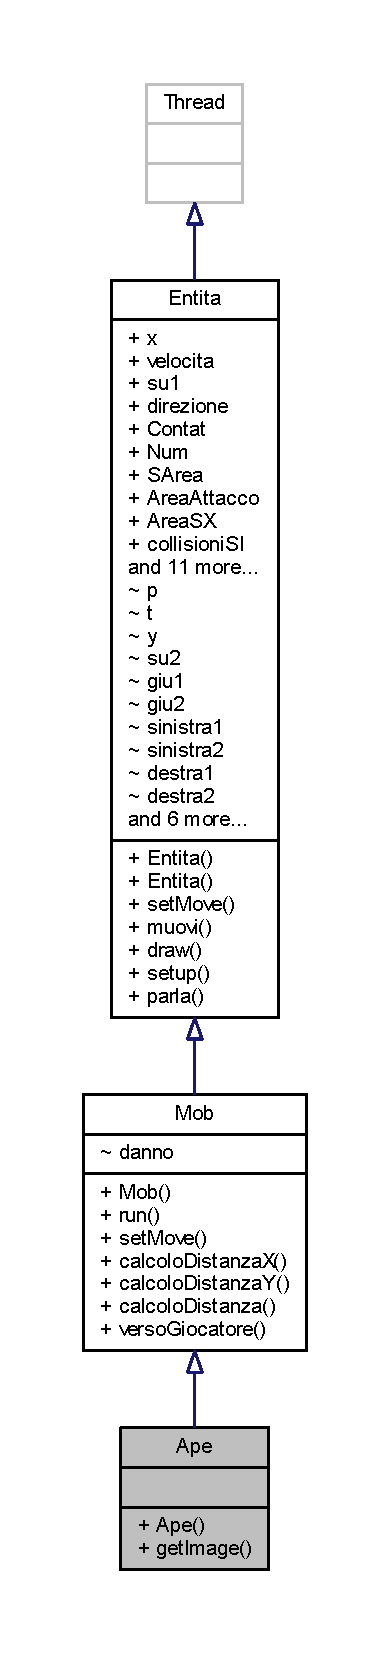
\includegraphics[height=550pt]{class_entita_1_1_ape__inherit__graph}
\end{center}
\end{figure}


Collaboration diagram for Ape\+:
\nopagebreak
\begin{figure}[H]
\begin{center}
\leavevmode
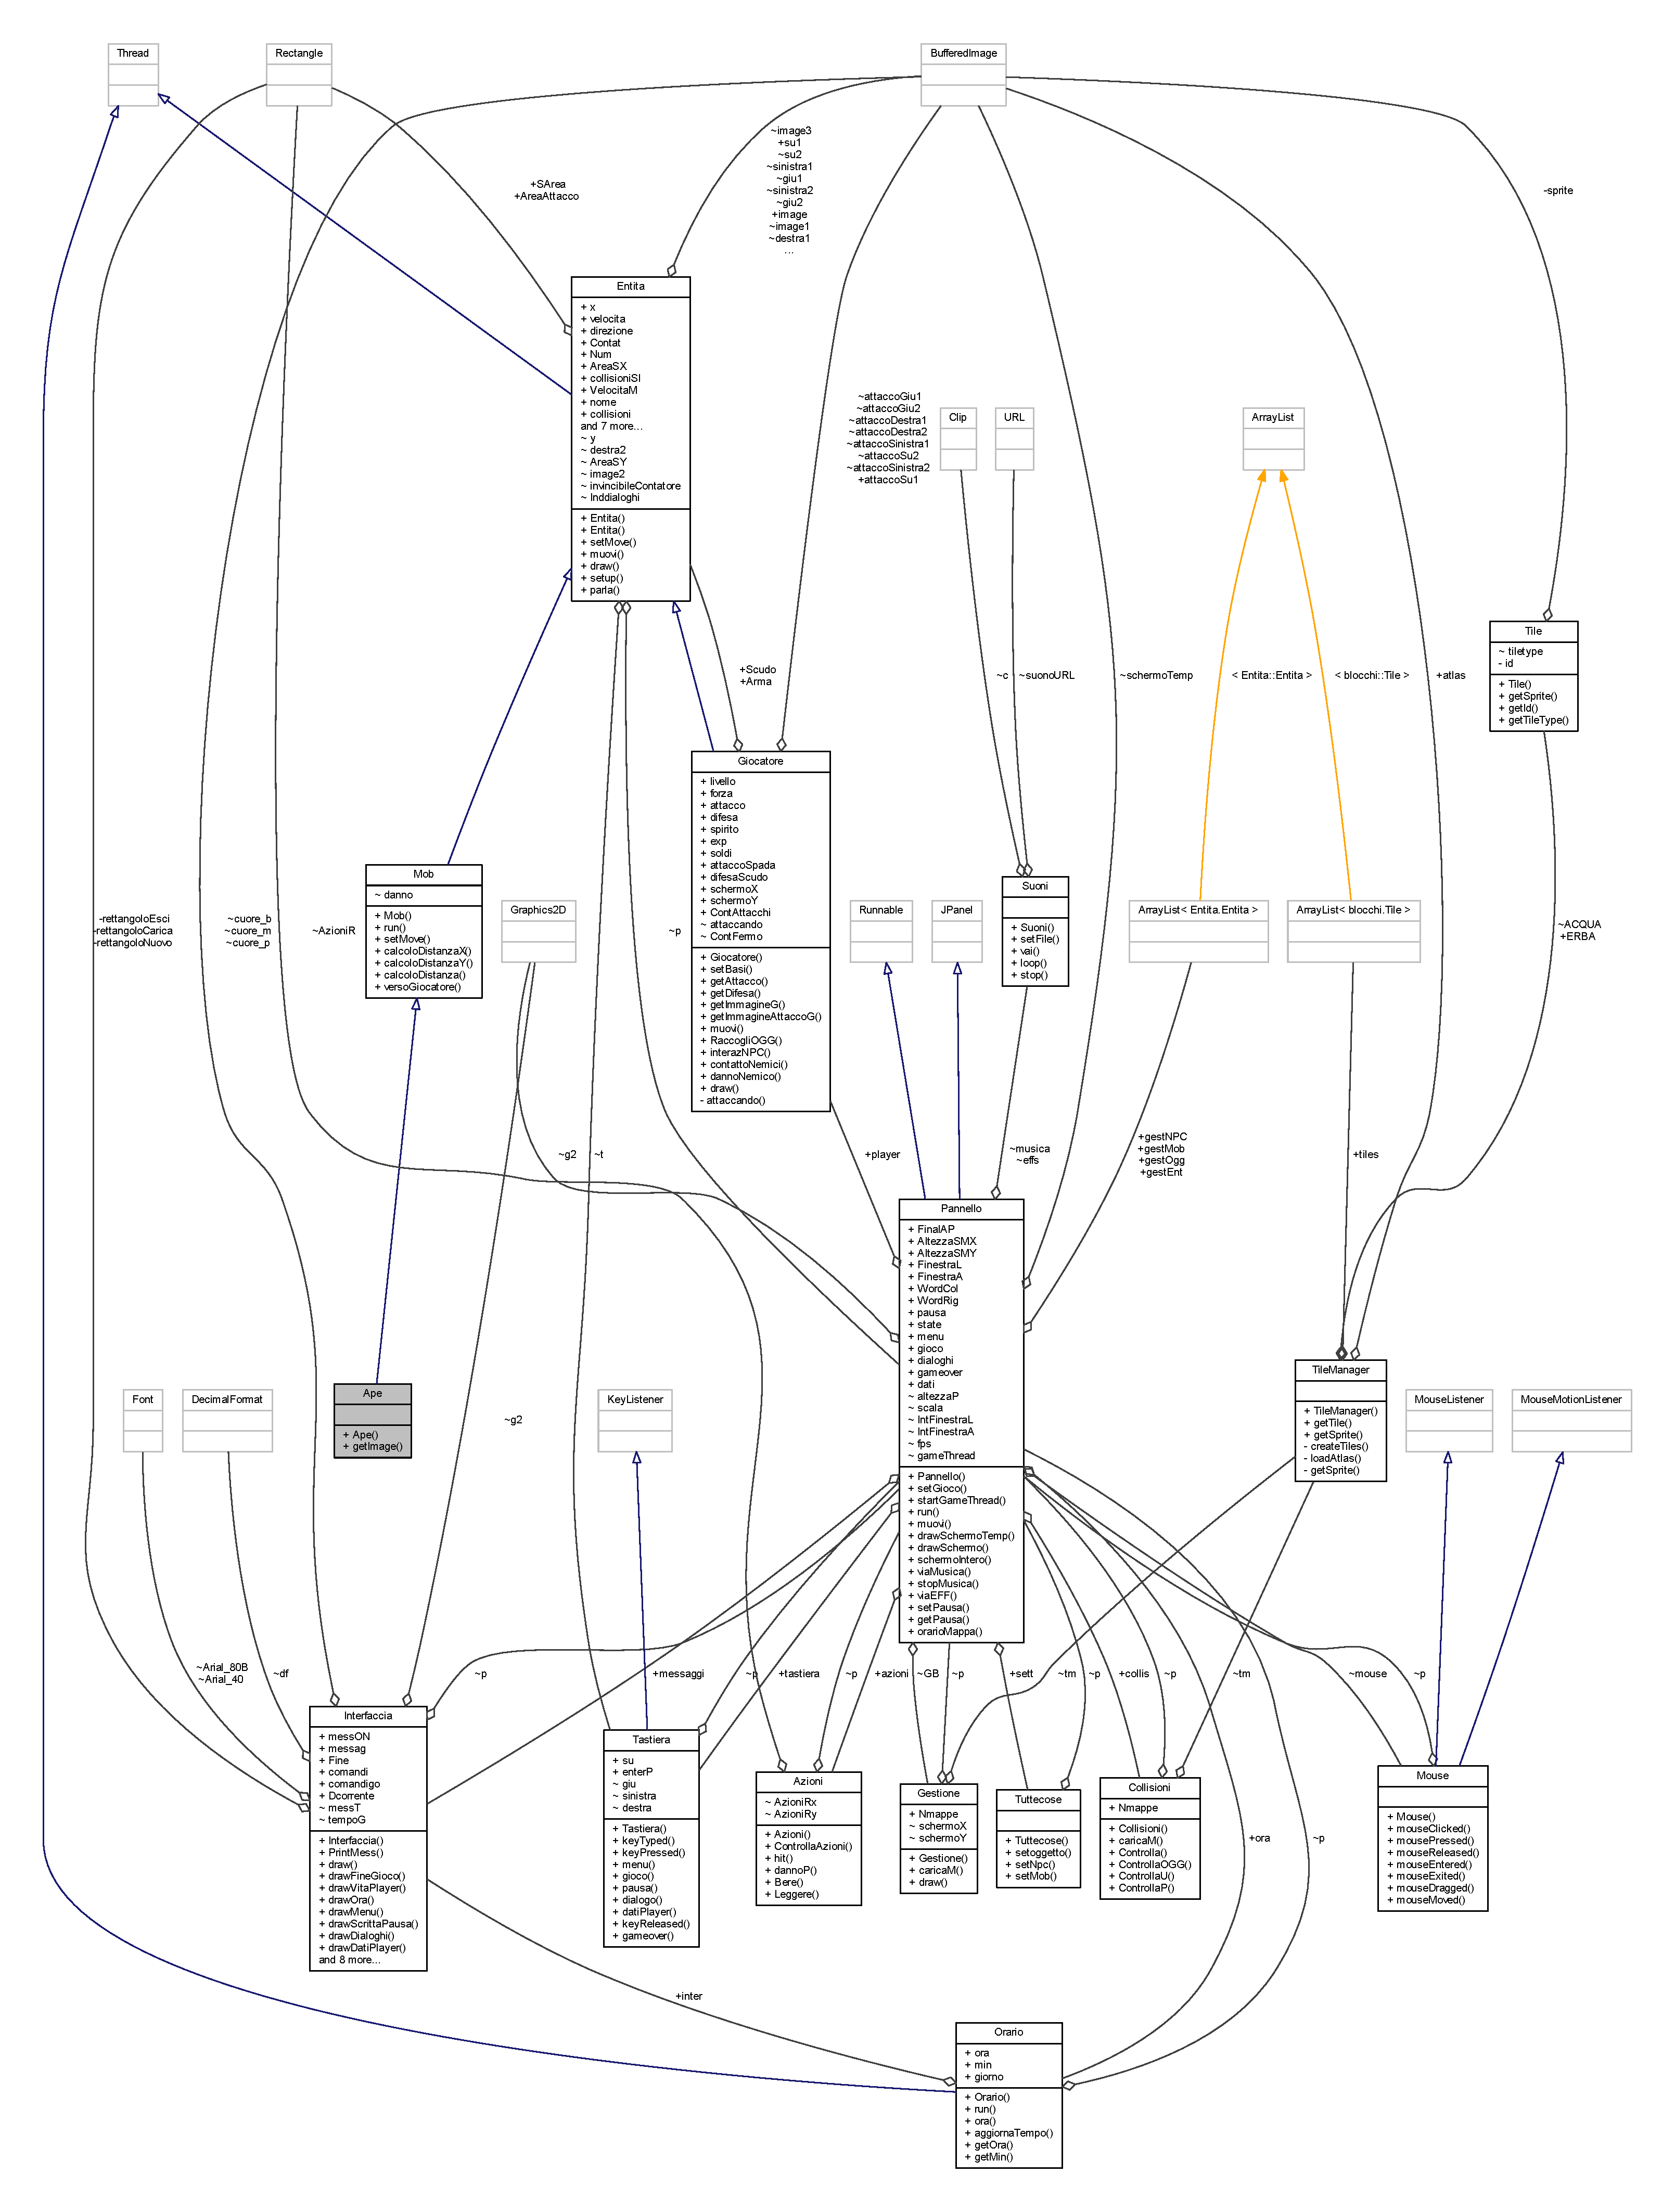
\includegraphics[width=350pt]{class_entita_1_1_ape__coll__graph}
\end{center}
\end{figure}
\subsection*{Public Member Functions}
\begin{DoxyCompactItemize}
\item 
\hyperlink{class_entita_1_1_ape_a5c67298368c58376888777816ca421d4}{Ape} (\hyperlink{classa_1_1survival_1_1game_1_1_pannello}{Pannello} p)
\begin{DoxyCompactList}\small\item\em Costruttore parametrico. \end{DoxyCompactList}\item 
void \hyperlink{class_entita_1_1_ape_acd4bd75c24769238f365de299bde96ac}{get\+Image} ()
\begin{DoxyCompactList}\small\item\em setto le immagini dell\textquotesingle{}ape \end{DoxyCompactList}\end{DoxyCompactItemize}
\subsection*{Additional Inherited Members}


\subsection{Detailed Description}
Classe con extends \hyperlink{class_entita_1_1_mob}{Mob}. 

Classe con extends Thread. 

Definition at line 16 of file Ape.\+java.



\subsection{Constructor \& Destructor Documentation}
\mbox{\Hypertarget{class_entita_1_1_ape_a5c67298368c58376888777816ca421d4}\label{class_entita_1_1_ape_a5c67298368c58376888777816ca421d4}} 
\index{Entita\+::\+Ape@{Entita\+::\+Ape}!Ape@{Ape}}
\index{Ape@{Ape}!Entita\+::\+Ape@{Entita\+::\+Ape}}
\subsubsection{\texorpdfstring{Ape()}{Ape()}}
{\footnotesize\ttfamily \hyperlink{class_entita_1_1_ape}{Ape} (\begin{DoxyParamCaption}\item[{\hyperlink{classa_1_1survival_1_1game_1_1_pannello}{Pannello}}]{p }\end{DoxyParamCaption})}



Costruttore parametrico. 


\begin{DoxyParams}{Parameters}
{\em p} & \\
\hline
\end{DoxyParams}
tipo npc

velocità ape

vita massima dell\textquotesingle{}ape

settaggi per Area collisioni

richiamo metodo get\+Image 

Definition at line 22 of file Ape.\+java.

Here is the call graph for this function\+:
\nopagebreak
\begin{figure}[H]
\begin{center}
\leavevmode
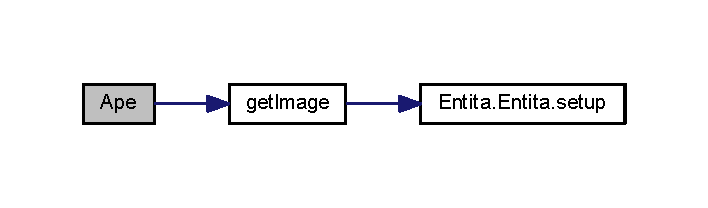
\includegraphics[width=340pt]{class_entita_1_1_ape_a5c67298368c58376888777816ca421d4_cgraph}
\end{center}
\end{figure}


\subsection{Member Function Documentation}
\mbox{\Hypertarget{class_entita_1_1_ape_acd4bd75c24769238f365de299bde96ac}\label{class_entita_1_1_ape_acd4bd75c24769238f365de299bde96ac}} 
\index{Entita\+::\+Ape@{Entita\+::\+Ape}!get\+Image@{get\+Image}}
\index{get\+Image@{get\+Image}!Entita\+::\+Ape@{Entita\+::\+Ape}}
\subsubsection{\texorpdfstring{get\+Image()}{getImage()}}
{\footnotesize\ttfamily void get\+Image (\begin{DoxyParamCaption}{ }\end{DoxyParamCaption})}



setto le immagini dell\textquotesingle{}ape 



Definition at line 45 of file Ape.\+java.

Here is the call graph for this function\+:
\nopagebreak
\begin{figure}[H]
\begin{center}
\leavevmode
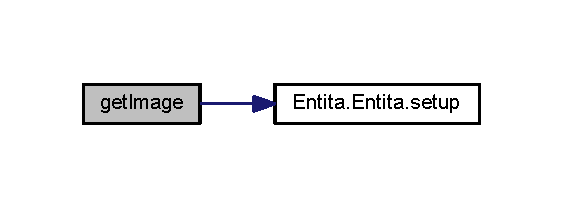
\includegraphics[width=270pt]{class_entita_1_1_ape_acd4bd75c24769238f365de299bde96ac_cgraph}
\end{center}
\end{figure}
Here is the caller graph for this function\+:
\nopagebreak
\begin{figure}[H]
\begin{center}
\leavevmode
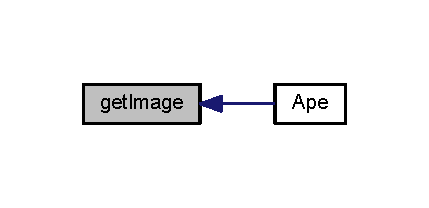
\includegraphics[width=206pt]{class_entita_1_1_ape_acd4bd75c24769238f365de299bde96ac_icgraph}
\end{center}
\end{figure}


The documentation for this class was generated from the following file\+:\begin{DoxyCompactItemize}
\item 
src/\+Entita/\hyperlink{_ape_8java}{Ape.\+java}\end{DoxyCompactItemize}

\hypertarget{classa_1_1survival_1_1game_1_1_a_survival_game}{}\section{A\+Survival\+Game Class Reference}
\label{classa_1_1survival_1_1game_1_1_a_survival_game}\index{A\+Survival\+Game@{A\+Survival\+Game}}


Collaboration diagram for A\+Survival\+Game\+:
\nopagebreak
\begin{figure}[H]
\begin{center}
\leavevmode
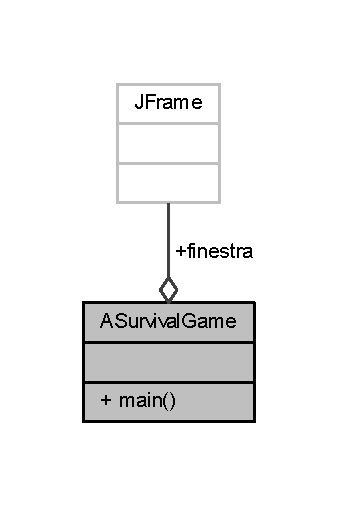
\includegraphics[width=162pt]{classa_1_1survival_1_1game_1_1_a_survival_game__coll__graph}
\end{center}
\end{figure}
\subsection*{Static Public Member Functions}
\begin{DoxyCompactItemize}
\item 
static void \hyperlink{classa_1_1survival_1_1game_1_1_a_survival_game_a8b260eecbaabcef8473fd87ada040682}{main} (String\mbox{[}$\,$\mbox{]} args)
\begin{DoxyCompactList}\small\item\em Classe main dove creo una J\+Frame con titolo e passo tutti i metodi che servono per avviare il gioco. \end{DoxyCompactList}\end{DoxyCompactItemize}
\subsection*{Static Public Attributes}
\begin{DoxyCompactItemize}
\item 
static J\+Frame \hyperlink{classa_1_1survival_1_1game_1_1_a_survival_game_a2566c4e674dd7ca4c0f6d0097845f6a6}{finestra}
\end{DoxyCompactItemize}


\subsection{Detailed Description}


Definition at line 15 of file A\+Survival\+Game.\+java.



\subsection{Member Function Documentation}
\mbox{\Hypertarget{classa_1_1survival_1_1game_1_1_a_survival_game_a8b260eecbaabcef8473fd87ada040682}\label{classa_1_1survival_1_1game_1_1_a_survival_game_a8b260eecbaabcef8473fd87ada040682}} 
\index{a\+::survival\+::game\+::\+A\+Survival\+Game@{a\+::survival\+::game\+::\+A\+Survival\+Game}!main@{main}}
\index{main@{main}!a\+::survival\+::game\+::\+A\+Survival\+Game@{a\+::survival\+::game\+::\+A\+Survival\+Game}}
\subsubsection{\texorpdfstring{main()}{main()}}
{\footnotesize\ttfamily static void main (\begin{DoxyParamCaption}\item[{String \mbox{[}$\,$\mbox{]}}]{args }\end{DoxyParamCaption})\hspace{0.3cm}{\ttfamily [static]}}



Classe main dove creo una J\+Frame con titolo e passo tutti i metodi che servono per avviare il gioco. 


\begin{DoxyParams}{Parameters}
{\em args} & \\
\hline
\end{DoxyParams}


Definition at line 24 of file A\+Survival\+Game.\+java.

Here is the call graph for this function\+:
\nopagebreak
\begin{figure}[H]
\begin{center}
\leavevmode
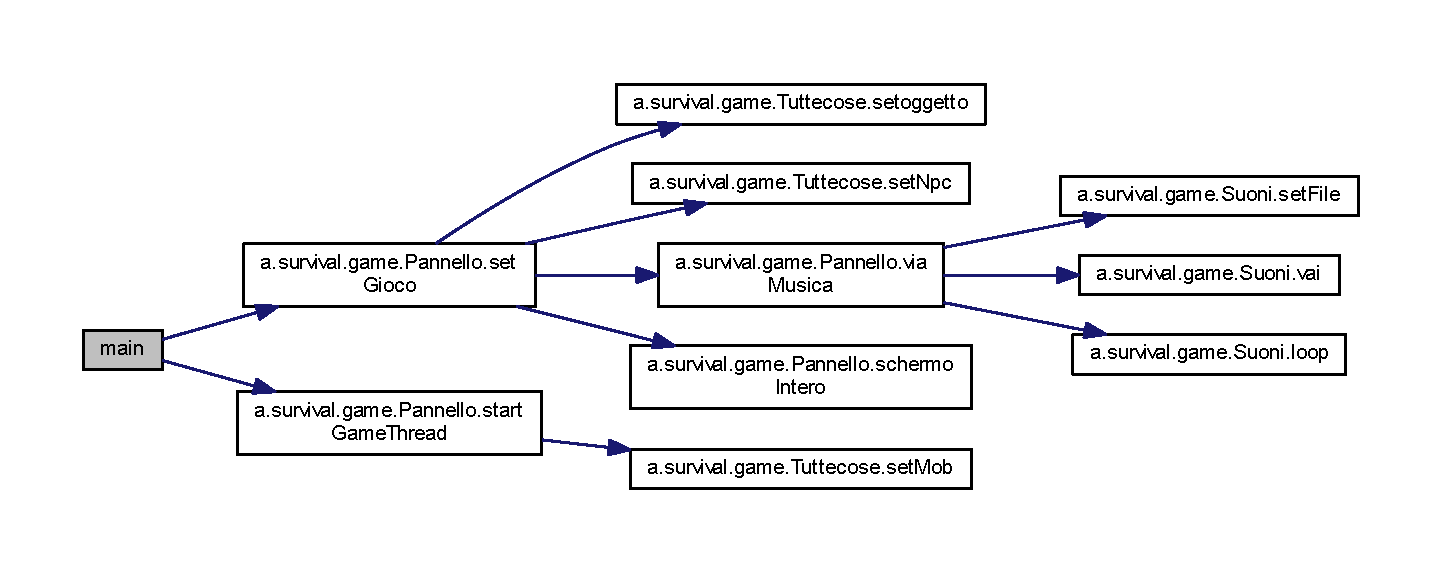
\includegraphics[width=350pt]{classa_1_1survival_1_1game_1_1_a_survival_game_a8b260eecbaabcef8473fd87ada040682_cgraph}
\end{center}
\end{figure}


\subsection{Member Data Documentation}
\mbox{\Hypertarget{classa_1_1survival_1_1game_1_1_a_survival_game_a2566c4e674dd7ca4c0f6d0097845f6a6}\label{classa_1_1survival_1_1game_1_1_a_survival_game_a2566c4e674dd7ca4c0f6d0097845f6a6}} 
\index{a\+::survival\+::game\+::\+A\+Survival\+Game@{a\+::survival\+::game\+::\+A\+Survival\+Game}!finestra@{finestra}}
\index{finestra@{finestra}!a\+::survival\+::game\+::\+A\+Survival\+Game@{a\+::survival\+::game\+::\+A\+Survival\+Game}}
\subsubsection{\texorpdfstring{finestra}{finestra}}
{\footnotesize\ttfamily J\+Frame finestra\hspace{0.3cm}{\ttfamily [static]}}

Creo J\+Frame 

Definition at line 18 of file A\+Survival\+Game.\+java.



The documentation for this class was generated from the following file\+:\begin{DoxyCompactItemize}
\item 
src/a/survival/game/\hyperlink{_a_survival_game_8java}{A\+Survival\+Game.\+java}\end{DoxyCompactItemize}

\hypertarget{classa_1_1survival_1_1game_1_1_azioni}{}\section{Azioni Class Reference}
\label{classa_1_1survival_1_1game_1_1_azioni}\index{Azioni@{Azioni}}


Collaboration diagram for Azioni\+:
\nopagebreak
\begin{figure}[H]
\begin{center}
\leavevmode
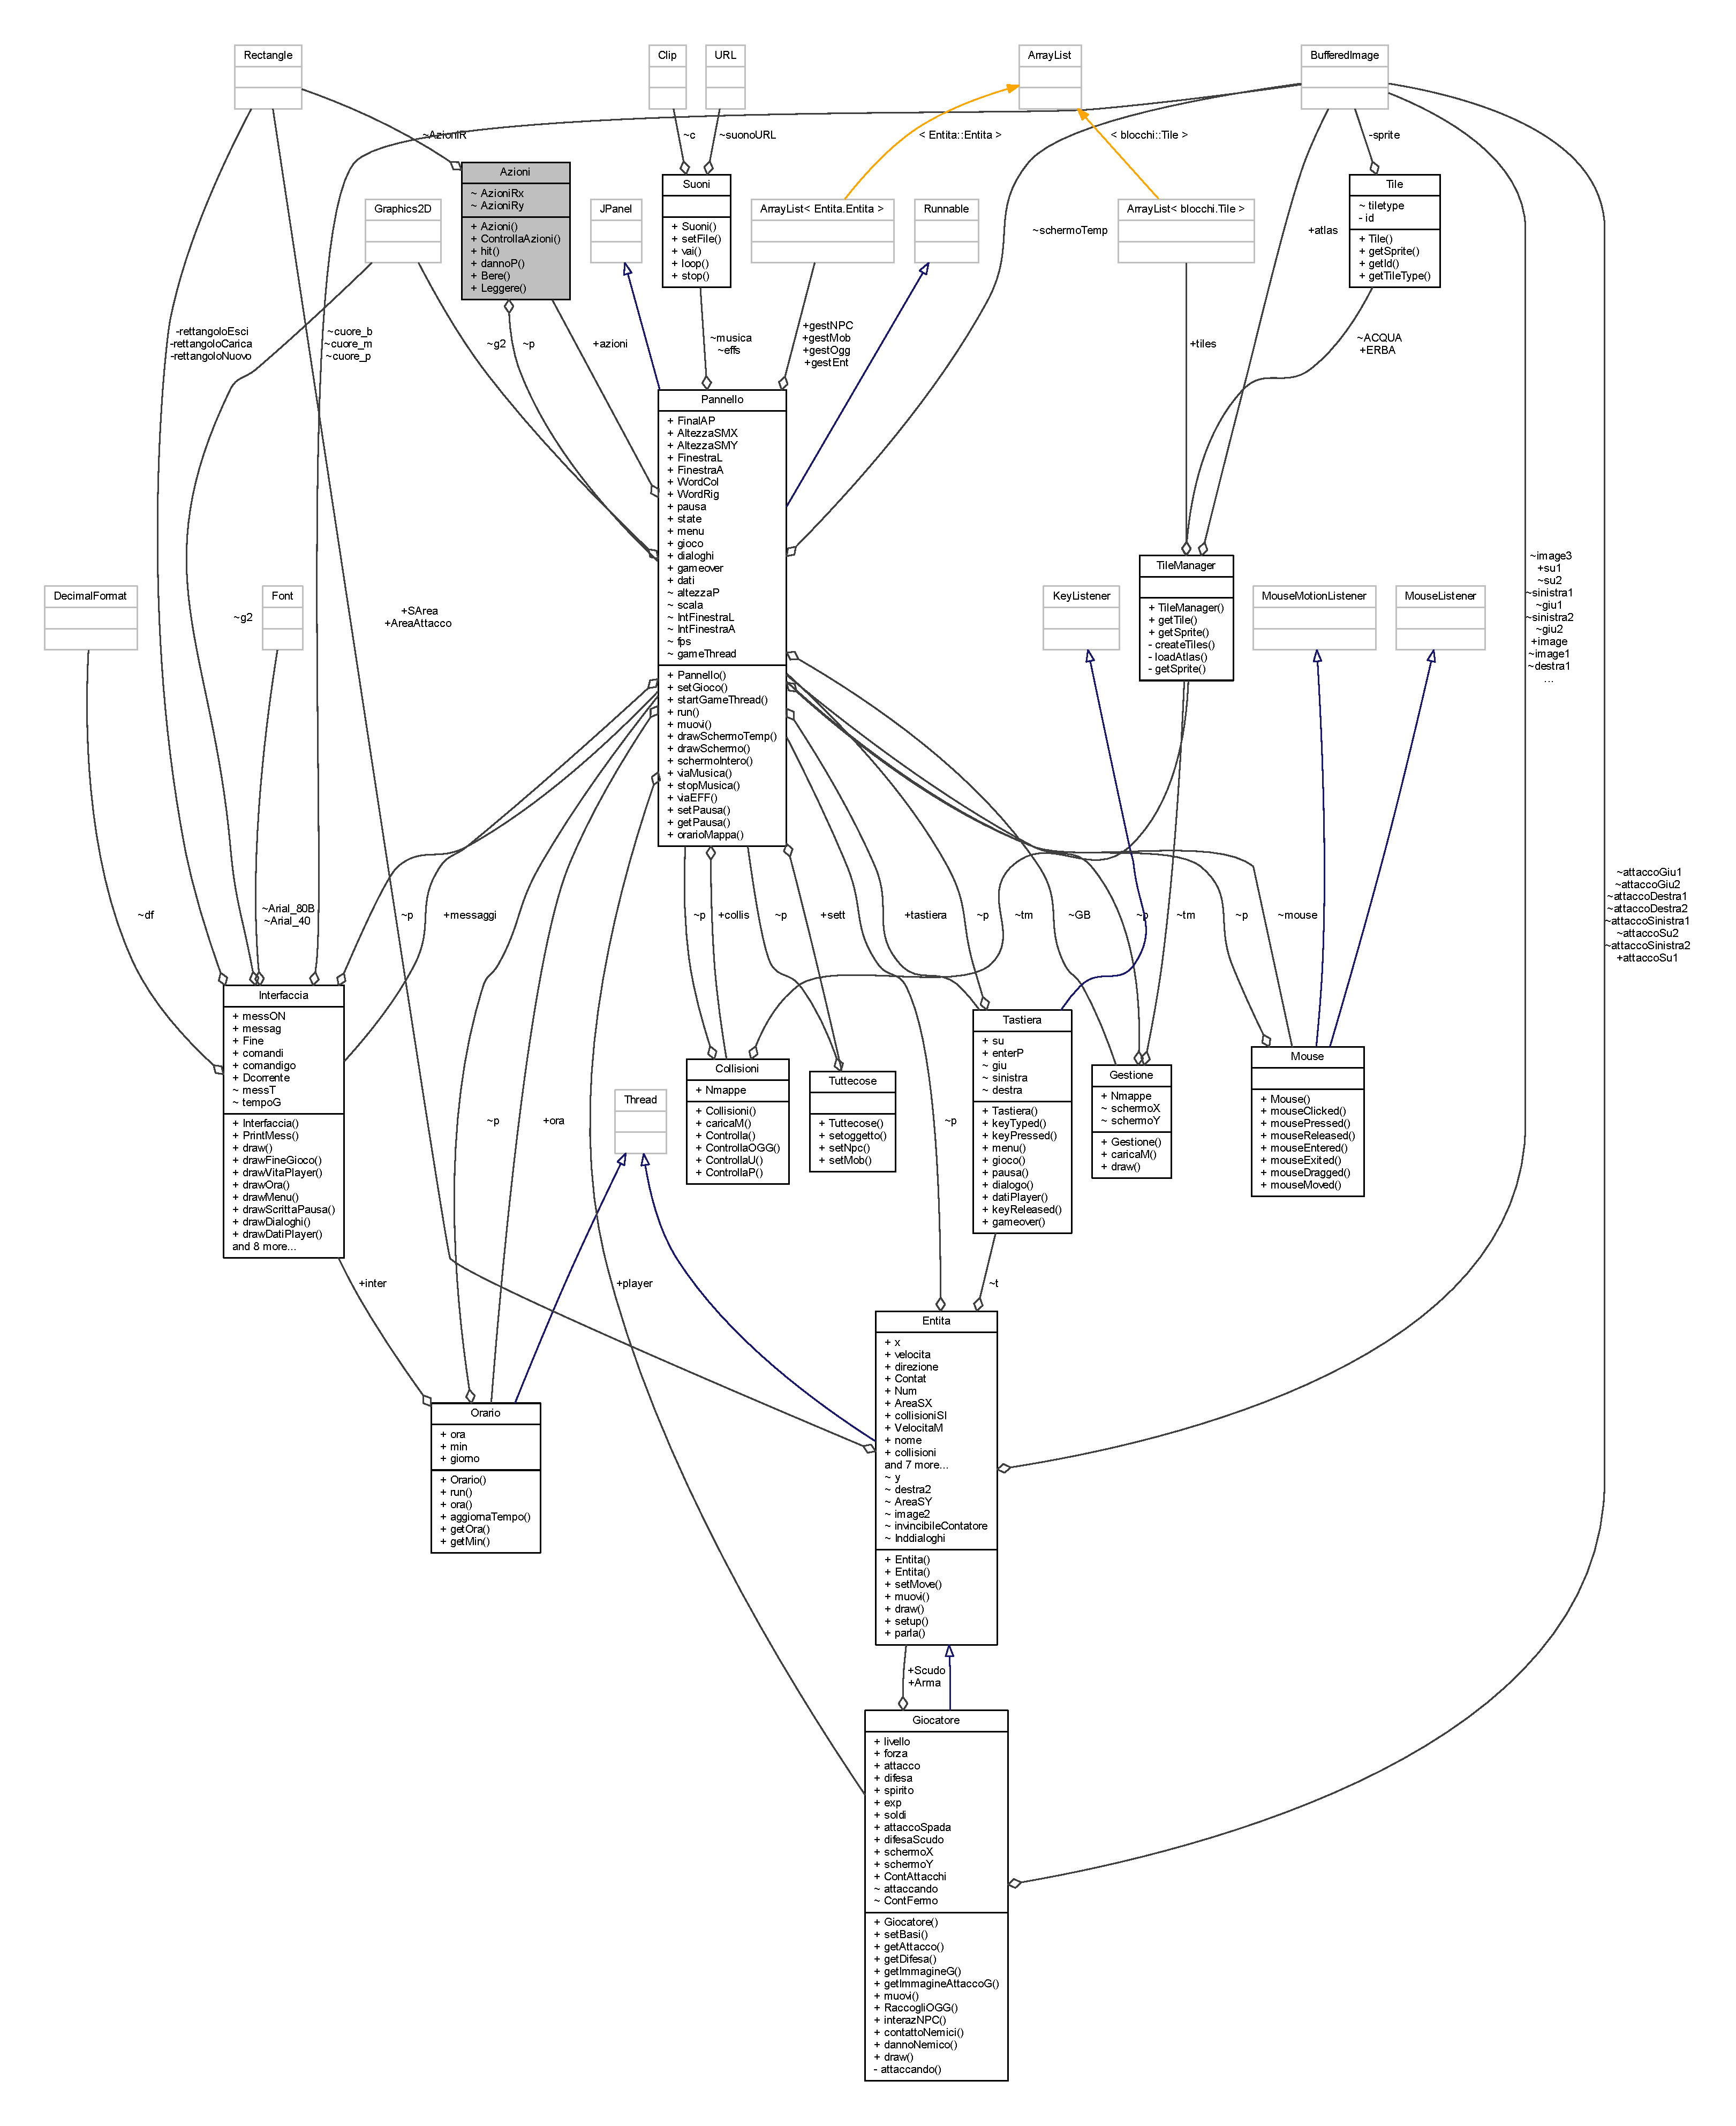
\includegraphics[width=350pt]{classa_1_1survival_1_1game_1_1_azioni__coll__graph}
\end{center}
\end{figure}
\subsection*{Public Member Functions}
\begin{DoxyCompactItemize}
\item 
\hyperlink{classa_1_1survival_1_1game_1_1_azioni_af521149b5bbecac98d09d33772e4bfd2}{Azioni} (\hyperlink{classa_1_1survival_1_1game_1_1_pannello}{Pannello} p)
\begin{DoxyCompactList}\small\item\em Costruttore parametrico. \end{DoxyCompactList}\item 
void \hyperlink{classa_1_1survival_1_1game_1_1_azioni_a39753d0160b9846cd1dd3d4556519456}{Controlla\+Azioni} ()
\begin{DoxyCompactList}\small\item\em setto un azione a 54$\ast$132 e se vado in quel blocco e premo invio allora printa il messaggio \end{DoxyCompactList}\item 
boolean \hyperlink{classa_1_1survival_1_1game_1_1_azioni_aa8b8a425d9f7a22d14cf64d6d0263927}{hit} (int Azionicol, int Azionirig, String direzione\+Ric)
\begin{DoxyCompactList}\small\item\em setto la x e la y dove posizionare l\textquotesingle{}azione \end{DoxyCompactList}\item 
void \hyperlink{classa_1_1survival_1_1game_1_1_azioni_ac1ebef3669e998cab686d462e5bdea24}{dannoP} (int Azione)
\begin{DoxyCompactList}\small\item\em Avendo un azione chiamata lava, questo metodo esiste per togliere vita al player se ci vado sopra. \end{DoxyCompactList}\item 
void \hyperlink{classa_1_1survival_1_1game_1_1_azioni_af6157da89a39a95e583e0bffc2da471d}{Bere} (int Azione)
\begin{DoxyCompactList}\small\item\em Avendo un azione chiamata bere, questo metodo esiste per recuperare vita al player se bevo acqua in un determinato punto. \end{DoxyCompactList}\item 
void \hyperlink{classa_1_1survival_1_1game_1_1_azioni_a9ca19225b144750b819e59fece5ef1a7}{Leggere} (int Azione)
\begin{DoxyCompactList}\small\item\em Avendo un azione chiamata cartello, questo metodo esiste per leggere le cose segnate sul oggetto cartello. \end{DoxyCompactList}\end{DoxyCompactItemize}


\subsection{Detailed Description}


Definition at line 15 of file Azioni.\+java.



\subsection{Constructor \& Destructor Documentation}
\mbox{\Hypertarget{classa_1_1survival_1_1game_1_1_azioni_af521149b5bbecac98d09d33772e4bfd2}\label{classa_1_1survival_1_1game_1_1_azioni_af521149b5bbecac98d09d33772e4bfd2}} 
\index{a\+::survival\+::game\+::\+Azioni@{a\+::survival\+::game\+::\+Azioni}!Azioni@{Azioni}}
\index{Azioni@{Azioni}!a\+::survival\+::game\+::\+Azioni@{a\+::survival\+::game\+::\+Azioni}}
\subsubsection{\texorpdfstring{Azioni()}{Azioni()}}
{\footnotesize\ttfamily \hyperlink{classa_1_1survival_1_1game_1_1_azioni}{Azioni} (\begin{DoxyParamCaption}\item[{\hyperlink{classa_1_1survival_1_1game_1_1_pannello}{Pannello}}]{p }\end{DoxyParamCaption})}



Costruttore parametrico. 


\begin{DoxyParams}{Parameters}
{\em p} & \\
\hline
\end{DoxyParams}


Definition at line 24 of file Azioni.\+java.



\subsection{Member Function Documentation}
\mbox{\Hypertarget{classa_1_1survival_1_1game_1_1_azioni_af6157da89a39a95e583e0bffc2da471d}\label{classa_1_1survival_1_1game_1_1_azioni_af6157da89a39a95e583e0bffc2da471d}} 
\index{a\+::survival\+::game\+::\+Azioni@{a\+::survival\+::game\+::\+Azioni}!Bere@{Bere}}
\index{Bere@{Bere}!a\+::survival\+::game\+::\+Azioni@{a\+::survival\+::game\+::\+Azioni}}
\subsubsection{\texorpdfstring{Bere()}{Bere()}}
{\footnotesize\ttfamily void Bere (\begin{DoxyParamCaption}\item[{int}]{Azione }\end{DoxyParamCaption})}



Avendo un azione chiamata bere, questo metodo esiste per recuperare vita al player se bevo acqua in un determinato punto. 


\begin{DoxyParams}{Parameters}
{\em Azione} & \\
\hline
\end{DoxyParams}


Definition at line 91 of file Azioni.\+java.

\mbox{\Hypertarget{classa_1_1survival_1_1game_1_1_azioni_a39753d0160b9846cd1dd3d4556519456}\label{classa_1_1survival_1_1game_1_1_azioni_a39753d0160b9846cd1dd3d4556519456}} 
\index{a\+::survival\+::game\+::\+Azioni@{a\+::survival\+::game\+::\+Azioni}!Controlla\+Azioni@{Controlla\+Azioni}}
\index{Controlla\+Azioni@{Controlla\+Azioni}!a\+::survival\+::game\+::\+Azioni@{a\+::survival\+::game\+::\+Azioni}}
\subsubsection{\texorpdfstring{Controlla\+Azioni()}{ControllaAzioni()}}
{\footnotesize\ttfamily void Controlla\+Azioni (\begin{DoxyParamCaption}{ }\end{DoxyParamCaption})}



setto un azione a 54$\ast$132 e se vado in quel blocco e premo invio allora printa il messaggio 



Definition at line 39 of file Azioni.\+java.

Here is the call graph for this function\+:
\nopagebreak
\begin{figure}[H]
\begin{center}
\leavevmode
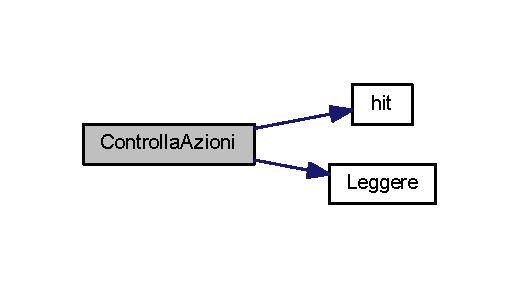
\includegraphics[width=249pt]{classa_1_1survival_1_1game_1_1_azioni_a39753d0160b9846cd1dd3d4556519456_cgraph}
\end{center}
\end{figure}
Here is the caller graph for this function\+:
\nopagebreak
\begin{figure}[H]
\begin{center}
\leavevmode
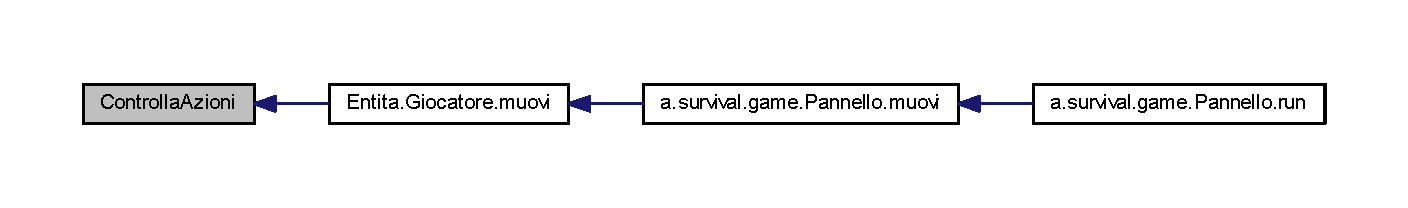
\includegraphics[width=350pt]{classa_1_1survival_1_1game_1_1_azioni_a39753d0160b9846cd1dd3d4556519456_icgraph}
\end{center}
\end{figure}
\mbox{\Hypertarget{classa_1_1survival_1_1game_1_1_azioni_ac1ebef3669e998cab686d462e5bdea24}\label{classa_1_1survival_1_1game_1_1_azioni_ac1ebef3669e998cab686d462e5bdea24}} 
\index{a\+::survival\+::game\+::\+Azioni@{a\+::survival\+::game\+::\+Azioni}!dannoP@{dannoP}}
\index{dannoP@{dannoP}!a\+::survival\+::game\+::\+Azioni@{a\+::survival\+::game\+::\+Azioni}}
\subsubsection{\texorpdfstring{danno\+P()}{dannoP()}}
{\footnotesize\ttfamily void dannoP (\begin{DoxyParamCaption}\item[{int}]{Azione }\end{DoxyParamCaption})}



Avendo un azione chiamata lava, questo metodo esiste per togliere vita al player se ci vado sopra. 


\begin{DoxyParams}{Parameters}
{\em Azione} & \\
\hline
\end{DoxyParams}


Definition at line 79 of file Azioni.\+java.

\mbox{\Hypertarget{classa_1_1survival_1_1game_1_1_azioni_aa8b8a425d9f7a22d14cf64d6d0263927}\label{classa_1_1survival_1_1game_1_1_azioni_aa8b8a425d9f7a22d14cf64d6d0263927}} 
\index{a\+::survival\+::game\+::\+Azioni@{a\+::survival\+::game\+::\+Azioni}!hit@{hit}}
\index{hit@{hit}!a\+::survival\+::game\+::\+Azioni@{a\+::survival\+::game\+::\+Azioni}}
\subsubsection{\texorpdfstring{hit()}{hit()}}
{\footnotesize\ttfamily boolean hit (\begin{DoxyParamCaption}\item[{int}]{Azionicol,  }\item[{int}]{Azionirig,  }\item[{String}]{direzione\+Ric }\end{DoxyParamCaption})}



setto la x e la y dove posizionare l\textquotesingle{}azione 


\begin{DoxyParams}{Parameters}
{\em Azionicol} & \\
\hline
{\em Azionirig} & \\
\hline
{\em direzione\+Ric} & \\
\hline
\end{DoxyParams}
\begin{DoxyReturn}{Returns}

\end{DoxyReturn}


Definition at line 54 of file Azioni.\+java.

Here is the caller graph for this function\+:
\nopagebreak
\begin{figure}[H]
\begin{center}
\leavevmode
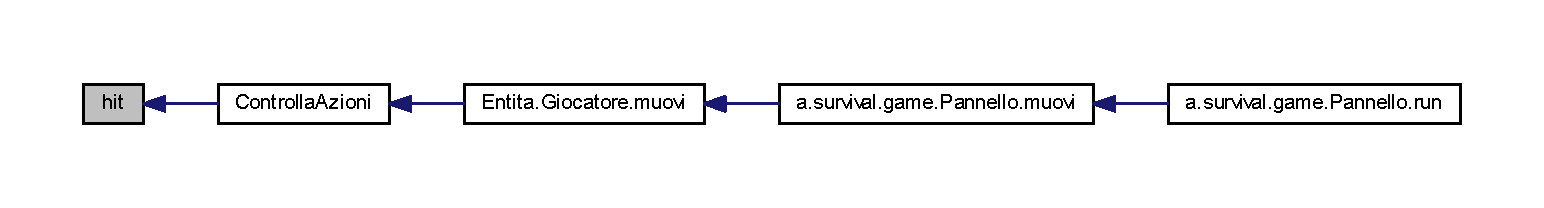
\includegraphics[width=350pt]{classa_1_1survival_1_1game_1_1_azioni_aa8b8a425d9f7a22d14cf64d6d0263927_icgraph}
\end{center}
\end{figure}
\mbox{\Hypertarget{classa_1_1survival_1_1game_1_1_azioni_a9ca19225b144750b819e59fece5ef1a7}\label{classa_1_1survival_1_1game_1_1_azioni_a9ca19225b144750b819e59fece5ef1a7}} 
\index{a\+::survival\+::game\+::\+Azioni@{a\+::survival\+::game\+::\+Azioni}!Leggere@{Leggere}}
\index{Leggere@{Leggere}!a\+::survival\+::game\+::\+Azioni@{a\+::survival\+::game\+::\+Azioni}}
\subsubsection{\texorpdfstring{Leggere()}{Leggere()}}
{\footnotesize\ttfamily void Leggere (\begin{DoxyParamCaption}\item[{int}]{Azione }\end{DoxyParamCaption})}



Avendo un azione chiamata cartello, questo metodo esiste per leggere le cose segnate sul oggetto cartello. 


\begin{DoxyParams}{Parameters}
{\em Azione} & \\
\hline
\end{DoxyParams}


Definition at line 106 of file Azioni.\+java.

Here is the caller graph for this function\+:
\nopagebreak
\begin{figure}[H]
\begin{center}
\leavevmode
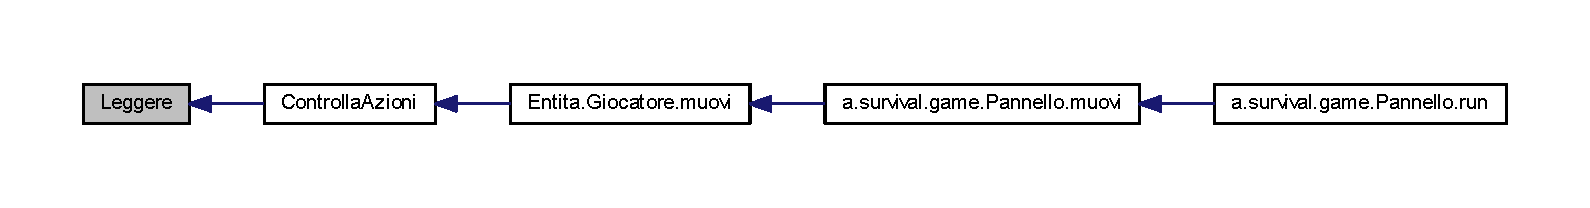
\includegraphics[width=350pt]{classa_1_1survival_1_1game_1_1_azioni_a9ca19225b144750b819e59fece5ef1a7_icgraph}
\end{center}
\end{figure}


The documentation for this class was generated from the following file\+:\begin{DoxyCompactItemize}
\item 
src/a/survival/game/\hyperlink{_azioni_8java}{Azioni.\+java}\end{DoxyCompactItemize}

\hypertarget{classa_1_1survival_1_1game_1_1_collisioni}{}\section{Collisioni Class Reference}
\label{classa_1_1survival_1_1game_1_1_collisioni}\index{Collisioni@{Collisioni}}


Collaboration diagram for Collisioni\+:
\nopagebreak
\begin{figure}[H]
\begin{center}
\leavevmode
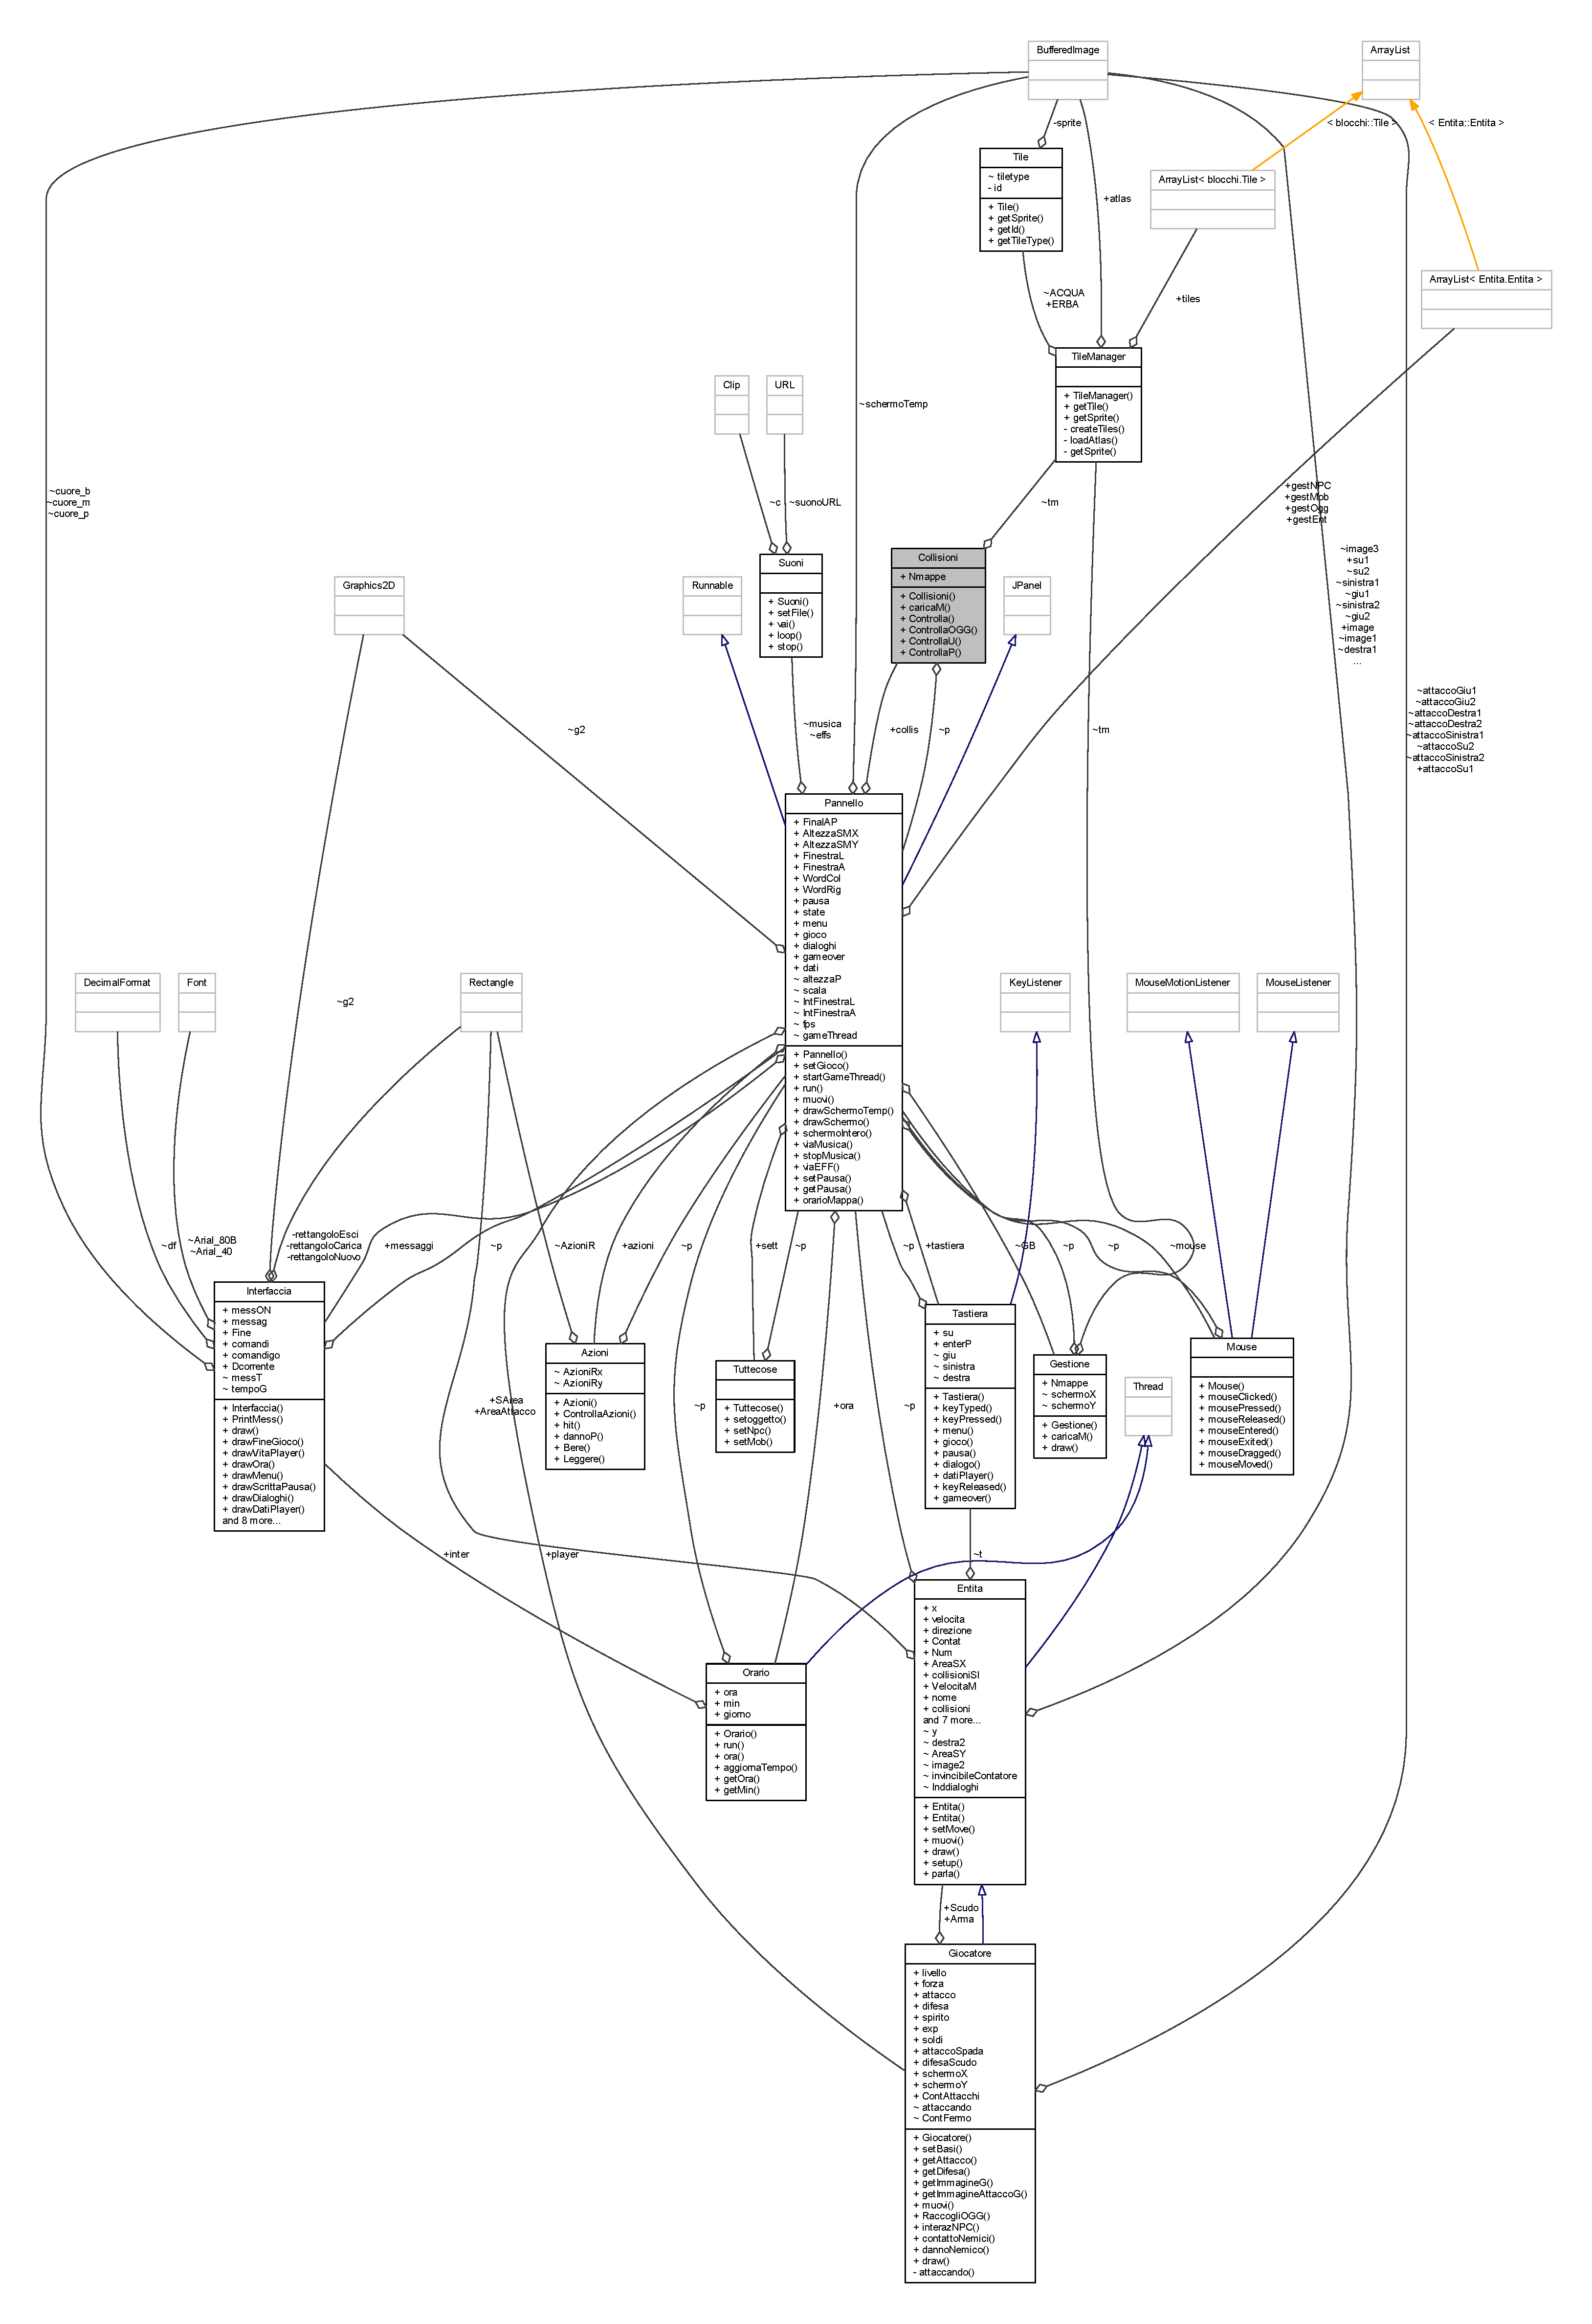
\includegraphics[width=350pt]{classa_1_1survival_1_1game_1_1_collisioni__coll__graph}
\end{center}
\end{figure}
\subsection*{Public Member Functions}
\begin{DoxyCompactItemize}
\item 
\hyperlink{classa_1_1survival_1_1game_1_1_collisioni_a65b3180595586bc591f7689883e01c7e}{Collisioni} (\hyperlink{classa_1_1survival_1_1game_1_1_pannello}{Pannello} p)
\item 
void \hyperlink{classa_1_1survival_1_1game_1_1_collisioni_a373d83d9b42d31e72ccc982a3fd85ea9}{caricaM} (String file)
\item 
void \hyperlink{classa_1_1survival_1_1game_1_1_collisioni_a839c38fa5d30f0458af3dcf4bf04f358}{Controlla} (\hyperlink{class_entita_1_1_entita}{Entita} e)
\item 
int \hyperlink{classa_1_1survival_1_1game_1_1_collisioni_ad38c8b3c50bbbd655ef3f9e2c80b21e0}{Controlla\+O\+GG} (\hyperlink{class_entita_1_1_entita}{Entita} u, boolean giocatore)
\item 
int \hyperlink{classa_1_1survival_1_1game_1_1_collisioni_a87a22cc62f824d7a4e9a017a9b36b019}{ControllaU} (\hyperlink{class_entita_1_1_entita}{Entita} e, Array\+List$<$ \hyperlink{class_entita_1_1_entita}{Entita} $>$ target)
\item 
boolean \hyperlink{classa_1_1survival_1_1game_1_1_collisioni_ab8b33fe794da631b2ee55f7b77bf31d5}{ControllaP} (\hyperlink{class_entita_1_1_entita}{Entita} e)
\end{DoxyCompactItemize}
\subsection*{Public Attributes}
\begin{DoxyCompactItemize}
\item 
int \hyperlink{classa_1_1survival_1_1game_1_1_collisioni_ac67a253aa050f8b036b79e9613b946e9}{Nmappe} \mbox{[}$\,$\mbox{]}\mbox{[}$\,$\mbox{]}
\end{DoxyCompactItemize}


\subsection{Detailed Description}
\begin{DoxyAuthor}{Author}
Denis 
\end{DoxyAuthor}


Definition at line 21 of file Collisioni.\+java.



\subsection{Constructor \& Destructor Documentation}
\mbox{\Hypertarget{classa_1_1survival_1_1game_1_1_collisioni_a65b3180595586bc591f7689883e01c7e}\label{classa_1_1survival_1_1game_1_1_collisioni_a65b3180595586bc591f7689883e01c7e}} 
\index{a\+::survival\+::game\+::\+Collisioni@{a\+::survival\+::game\+::\+Collisioni}!Collisioni@{Collisioni}}
\index{Collisioni@{Collisioni}!a\+::survival\+::game\+::\+Collisioni@{a\+::survival\+::game\+::\+Collisioni}}
\subsubsection{\texorpdfstring{Collisioni()}{Collisioni()}}
{\footnotesize\ttfamily \hyperlink{classa_1_1survival_1_1game_1_1_collisioni}{Collisioni} (\begin{DoxyParamCaption}\item[{\hyperlink{classa_1_1survival_1_1game_1_1_pannello}{Pannello}}]{p }\end{DoxyParamCaption})}



Definition at line 26 of file Collisioni.\+java.

Here is the call graph for this function\+:
\nopagebreak
\begin{figure}[H]
\begin{center}
\leavevmode
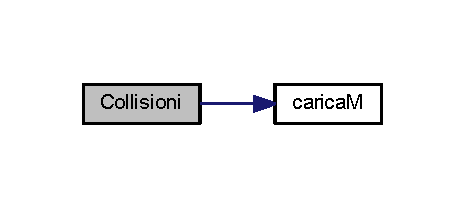
\includegraphics[width=223pt]{classa_1_1survival_1_1game_1_1_collisioni_a65b3180595586bc591f7689883e01c7e_cgraph}
\end{center}
\end{figure}


\subsection{Member Function Documentation}
\mbox{\Hypertarget{classa_1_1survival_1_1game_1_1_collisioni_a373d83d9b42d31e72ccc982a3fd85ea9}\label{classa_1_1survival_1_1game_1_1_collisioni_a373d83d9b42d31e72ccc982a3fd85ea9}} 
\index{a\+::survival\+::game\+::\+Collisioni@{a\+::survival\+::game\+::\+Collisioni}!caricaM@{caricaM}}
\index{caricaM@{caricaM}!a\+::survival\+::game\+::\+Collisioni@{a\+::survival\+::game\+::\+Collisioni}}
\subsubsection{\texorpdfstring{carica\+M()}{caricaM()}}
{\footnotesize\ttfamily void caricaM (\begin{DoxyParamCaption}\item[{String}]{file }\end{DoxyParamCaption})}



Definition at line 37 of file Collisioni.\+java.

Here is the caller graph for this function\+:
\nopagebreak
\begin{figure}[H]
\begin{center}
\leavevmode
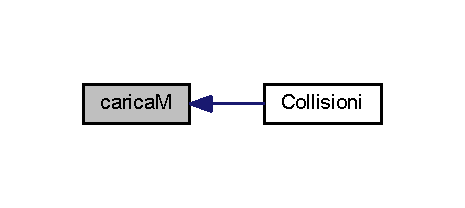
\includegraphics[width=223pt]{classa_1_1survival_1_1game_1_1_collisioni_a373d83d9b42d31e72ccc982a3fd85ea9_icgraph}
\end{center}
\end{figure}
\mbox{\Hypertarget{classa_1_1survival_1_1game_1_1_collisioni_a839c38fa5d30f0458af3dcf4bf04f358}\label{classa_1_1survival_1_1game_1_1_collisioni_a839c38fa5d30f0458af3dcf4bf04f358}} 
\index{a\+::survival\+::game\+::\+Collisioni@{a\+::survival\+::game\+::\+Collisioni}!Controlla@{Controlla}}
\index{Controlla@{Controlla}!a\+::survival\+::game\+::\+Collisioni@{a\+::survival\+::game\+::\+Collisioni}}
\subsubsection{\texorpdfstring{Controlla()}{Controlla()}}
{\footnotesize\ttfamily void Controlla (\begin{DoxyParamCaption}\item[{\hyperlink{class_entita_1_1_entita}{Entita}}]{e }\end{DoxyParamCaption})}



Definition at line 62 of file Collisioni.\+java.

Here is the call graph for this function\+:
\nopagebreak
\begin{figure}[H]
\begin{center}
\leavevmode
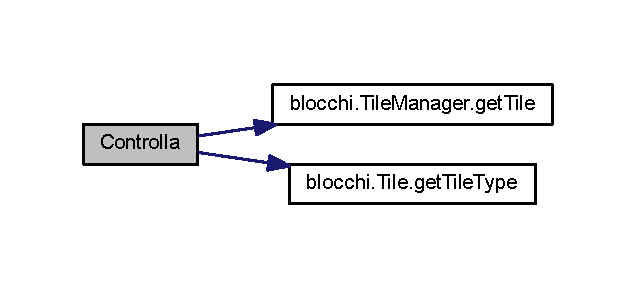
\includegraphics[width=305pt]{classa_1_1survival_1_1game_1_1_collisioni_a839c38fa5d30f0458af3dcf4bf04f358_cgraph}
\end{center}
\end{figure}
Here is the caller graph for this function\+:
\nopagebreak
\begin{figure}[H]
\begin{center}
\leavevmode
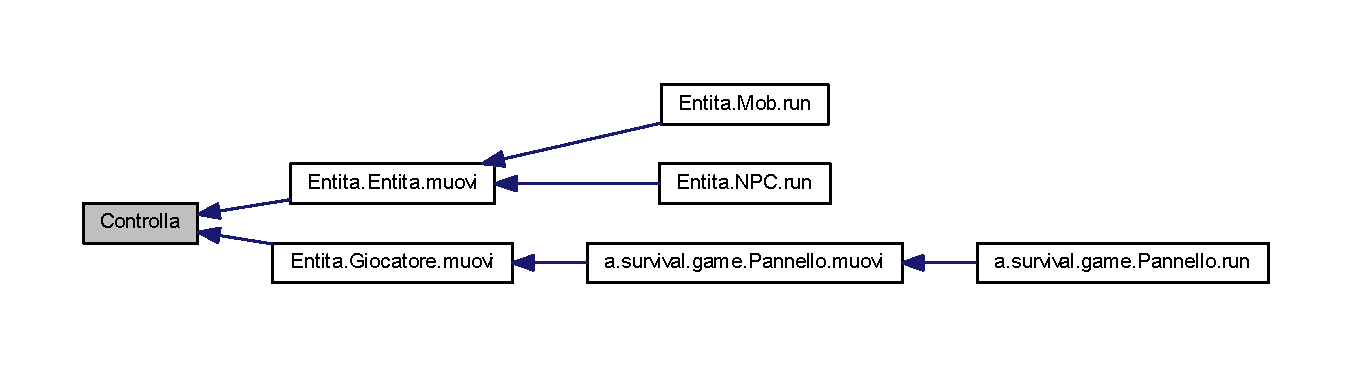
\includegraphics[width=350pt]{classa_1_1survival_1_1game_1_1_collisioni_a839c38fa5d30f0458af3dcf4bf04f358_icgraph}
\end{center}
\end{figure}
\mbox{\Hypertarget{classa_1_1survival_1_1game_1_1_collisioni_ad38c8b3c50bbbd655ef3f9e2c80b21e0}\label{classa_1_1survival_1_1game_1_1_collisioni_ad38c8b3c50bbbd655ef3f9e2c80b21e0}} 
\index{a\+::survival\+::game\+::\+Collisioni@{a\+::survival\+::game\+::\+Collisioni}!Controlla\+O\+GG@{Controlla\+O\+GG}}
\index{Controlla\+O\+GG@{Controlla\+O\+GG}!a\+::survival\+::game\+::\+Collisioni@{a\+::survival\+::game\+::\+Collisioni}}
\subsubsection{\texorpdfstring{Controlla\+O\+G\+G()}{ControllaOGG()}}
{\footnotesize\ttfamily int Controlla\+O\+GG (\begin{DoxyParamCaption}\item[{\hyperlink{class_entita_1_1_entita}{Entita}}]{u,  }\item[{boolean}]{giocatore }\end{DoxyParamCaption})}



Definition at line 92 of file Collisioni.\+java.

Here is the caller graph for this function\+:
\nopagebreak
\begin{figure}[H]
\begin{center}
\leavevmode
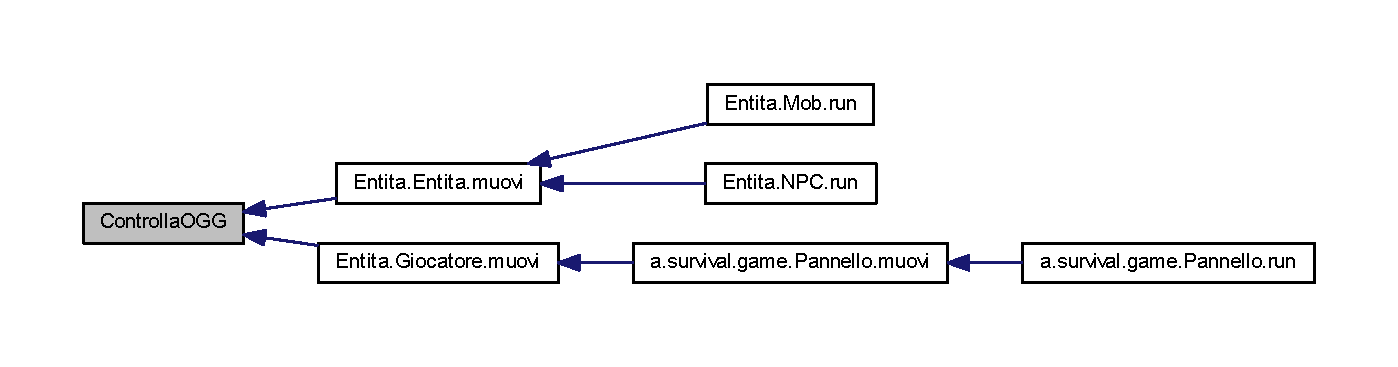
\includegraphics[width=350pt]{classa_1_1survival_1_1game_1_1_collisioni_ad38c8b3c50bbbd655ef3f9e2c80b21e0_icgraph}
\end{center}
\end{figure}
\mbox{\Hypertarget{classa_1_1survival_1_1game_1_1_collisioni_ab8b33fe794da631b2ee55f7b77bf31d5}\label{classa_1_1survival_1_1game_1_1_collisioni_ab8b33fe794da631b2ee55f7b77bf31d5}} 
\index{a\+::survival\+::game\+::\+Collisioni@{a\+::survival\+::game\+::\+Collisioni}!ControllaP@{ControllaP}}
\index{ControllaP@{ControllaP}!a\+::survival\+::game\+::\+Collisioni@{a\+::survival\+::game\+::\+Collisioni}}
\subsubsection{\texorpdfstring{Controlla\+P()}{ControllaP()}}
{\footnotesize\ttfamily boolean ControllaP (\begin{DoxyParamCaption}\item[{\hyperlink{class_entita_1_1_entita}{Entita}}]{e }\end{DoxyParamCaption})}



Definition at line 167 of file Collisioni.\+java.

Here is the caller graph for this function\+:
\nopagebreak
\begin{figure}[H]
\begin{center}
\leavevmode
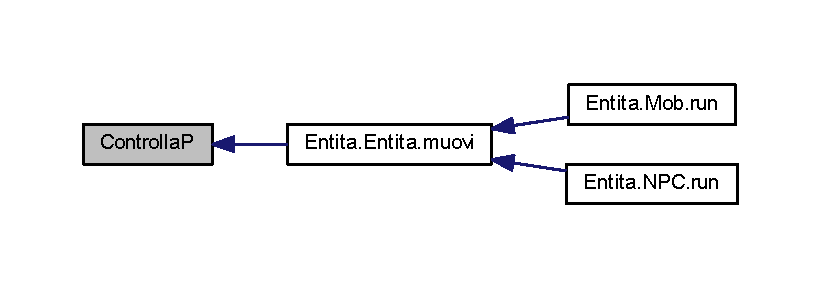
\includegraphics[width=350pt]{classa_1_1survival_1_1game_1_1_collisioni_ab8b33fe794da631b2ee55f7b77bf31d5_icgraph}
\end{center}
\end{figure}
\mbox{\Hypertarget{classa_1_1survival_1_1game_1_1_collisioni_a87a22cc62f824d7a4e9a017a9b36b019}\label{classa_1_1survival_1_1game_1_1_collisioni_a87a22cc62f824d7a4e9a017a9b36b019}} 
\index{a\+::survival\+::game\+::\+Collisioni@{a\+::survival\+::game\+::\+Collisioni}!ControllaU@{ControllaU}}
\index{ControllaU@{ControllaU}!a\+::survival\+::game\+::\+Collisioni@{a\+::survival\+::game\+::\+Collisioni}}
\subsubsection{\texorpdfstring{Controlla\+U()}{ControllaU()}}
{\footnotesize\ttfamily int ControllaU (\begin{DoxyParamCaption}\item[{\hyperlink{class_entita_1_1_entita}{Entita}}]{e,  }\item[{Array\+List$<$ \hyperlink{class_entita_1_1_entita}{Entita} $>$}]{target }\end{DoxyParamCaption})}



Definition at line 128 of file Collisioni.\+java.

Here is the caller graph for this function\+:
\nopagebreak
\begin{figure}[H]
\begin{center}
\leavevmode
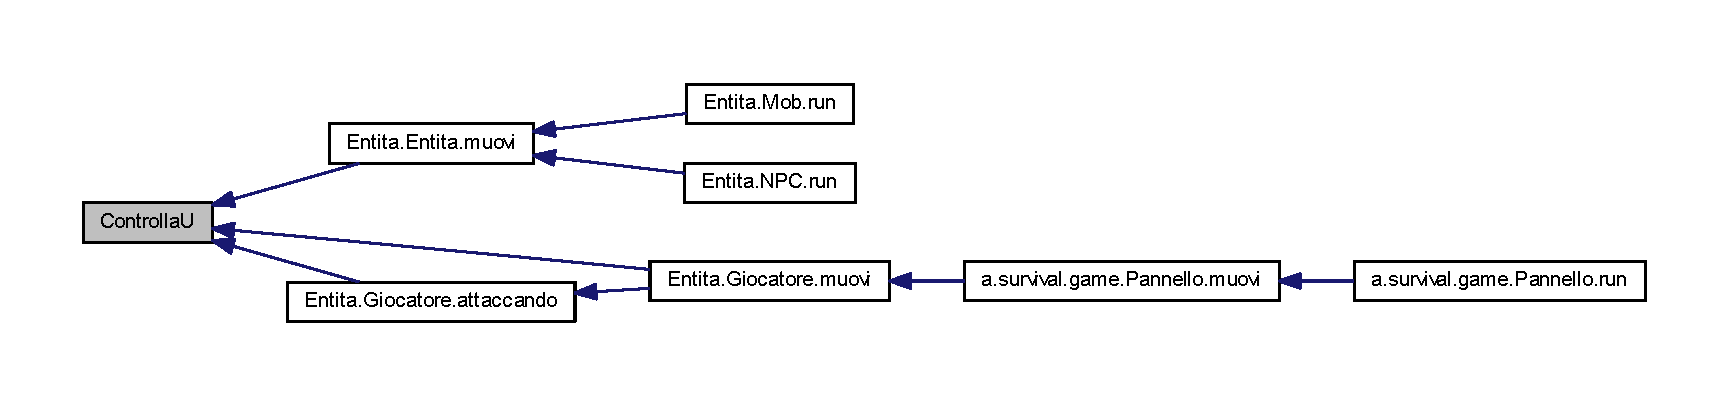
\includegraphics[width=350pt]{classa_1_1survival_1_1game_1_1_collisioni_a87a22cc62f824d7a4e9a017a9b36b019_icgraph}
\end{center}
\end{figure}


\subsection{Member Data Documentation}
\mbox{\Hypertarget{classa_1_1survival_1_1game_1_1_collisioni_ac67a253aa050f8b036b79e9613b946e9}\label{classa_1_1survival_1_1game_1_1_collisioni_ac67a253aa050f8b036b79e9613b946e9}} 
\index{a\+::survival\+::game\+::\+Collisioni@{a\+::survival\+::game\+::\+Collisioni}!Nmappe@{Nmappe}}
\index{Nmappe@{Nmappe}!a\+::survival\+::game\+::\+Collisioni@{a\+::survival\+::game\+::\+Collisioni}}
\subsubsection{\texorpdfstring{Nmappe}{Nmappe}}
{\footnotesize\ttfamily int Nmappe\mbox{[}$\,$\mbox{]}\mbox{[}$\,$\mbox{]}}



Definition at line 23 of file Collisioni.\+java.



The documentation for this class was generated from the following file\+:\begin{DoxyCompactItemize}
\item 
src/a/survival/game/\hyperlink{_collisioni_8java}{Collisioni.\+java}\end{DoxyCompactItemize}

\hypertarget{class_entita_1_1_entita}{}\section{Entita Class Reference}
\label{class_entita_1_1_entita}\index{Entita@{Entita}}


Inheritance diagram for Entita\+:
\nopagebreak
\begin{figure}[H]
\begin{center}
\leavevmode
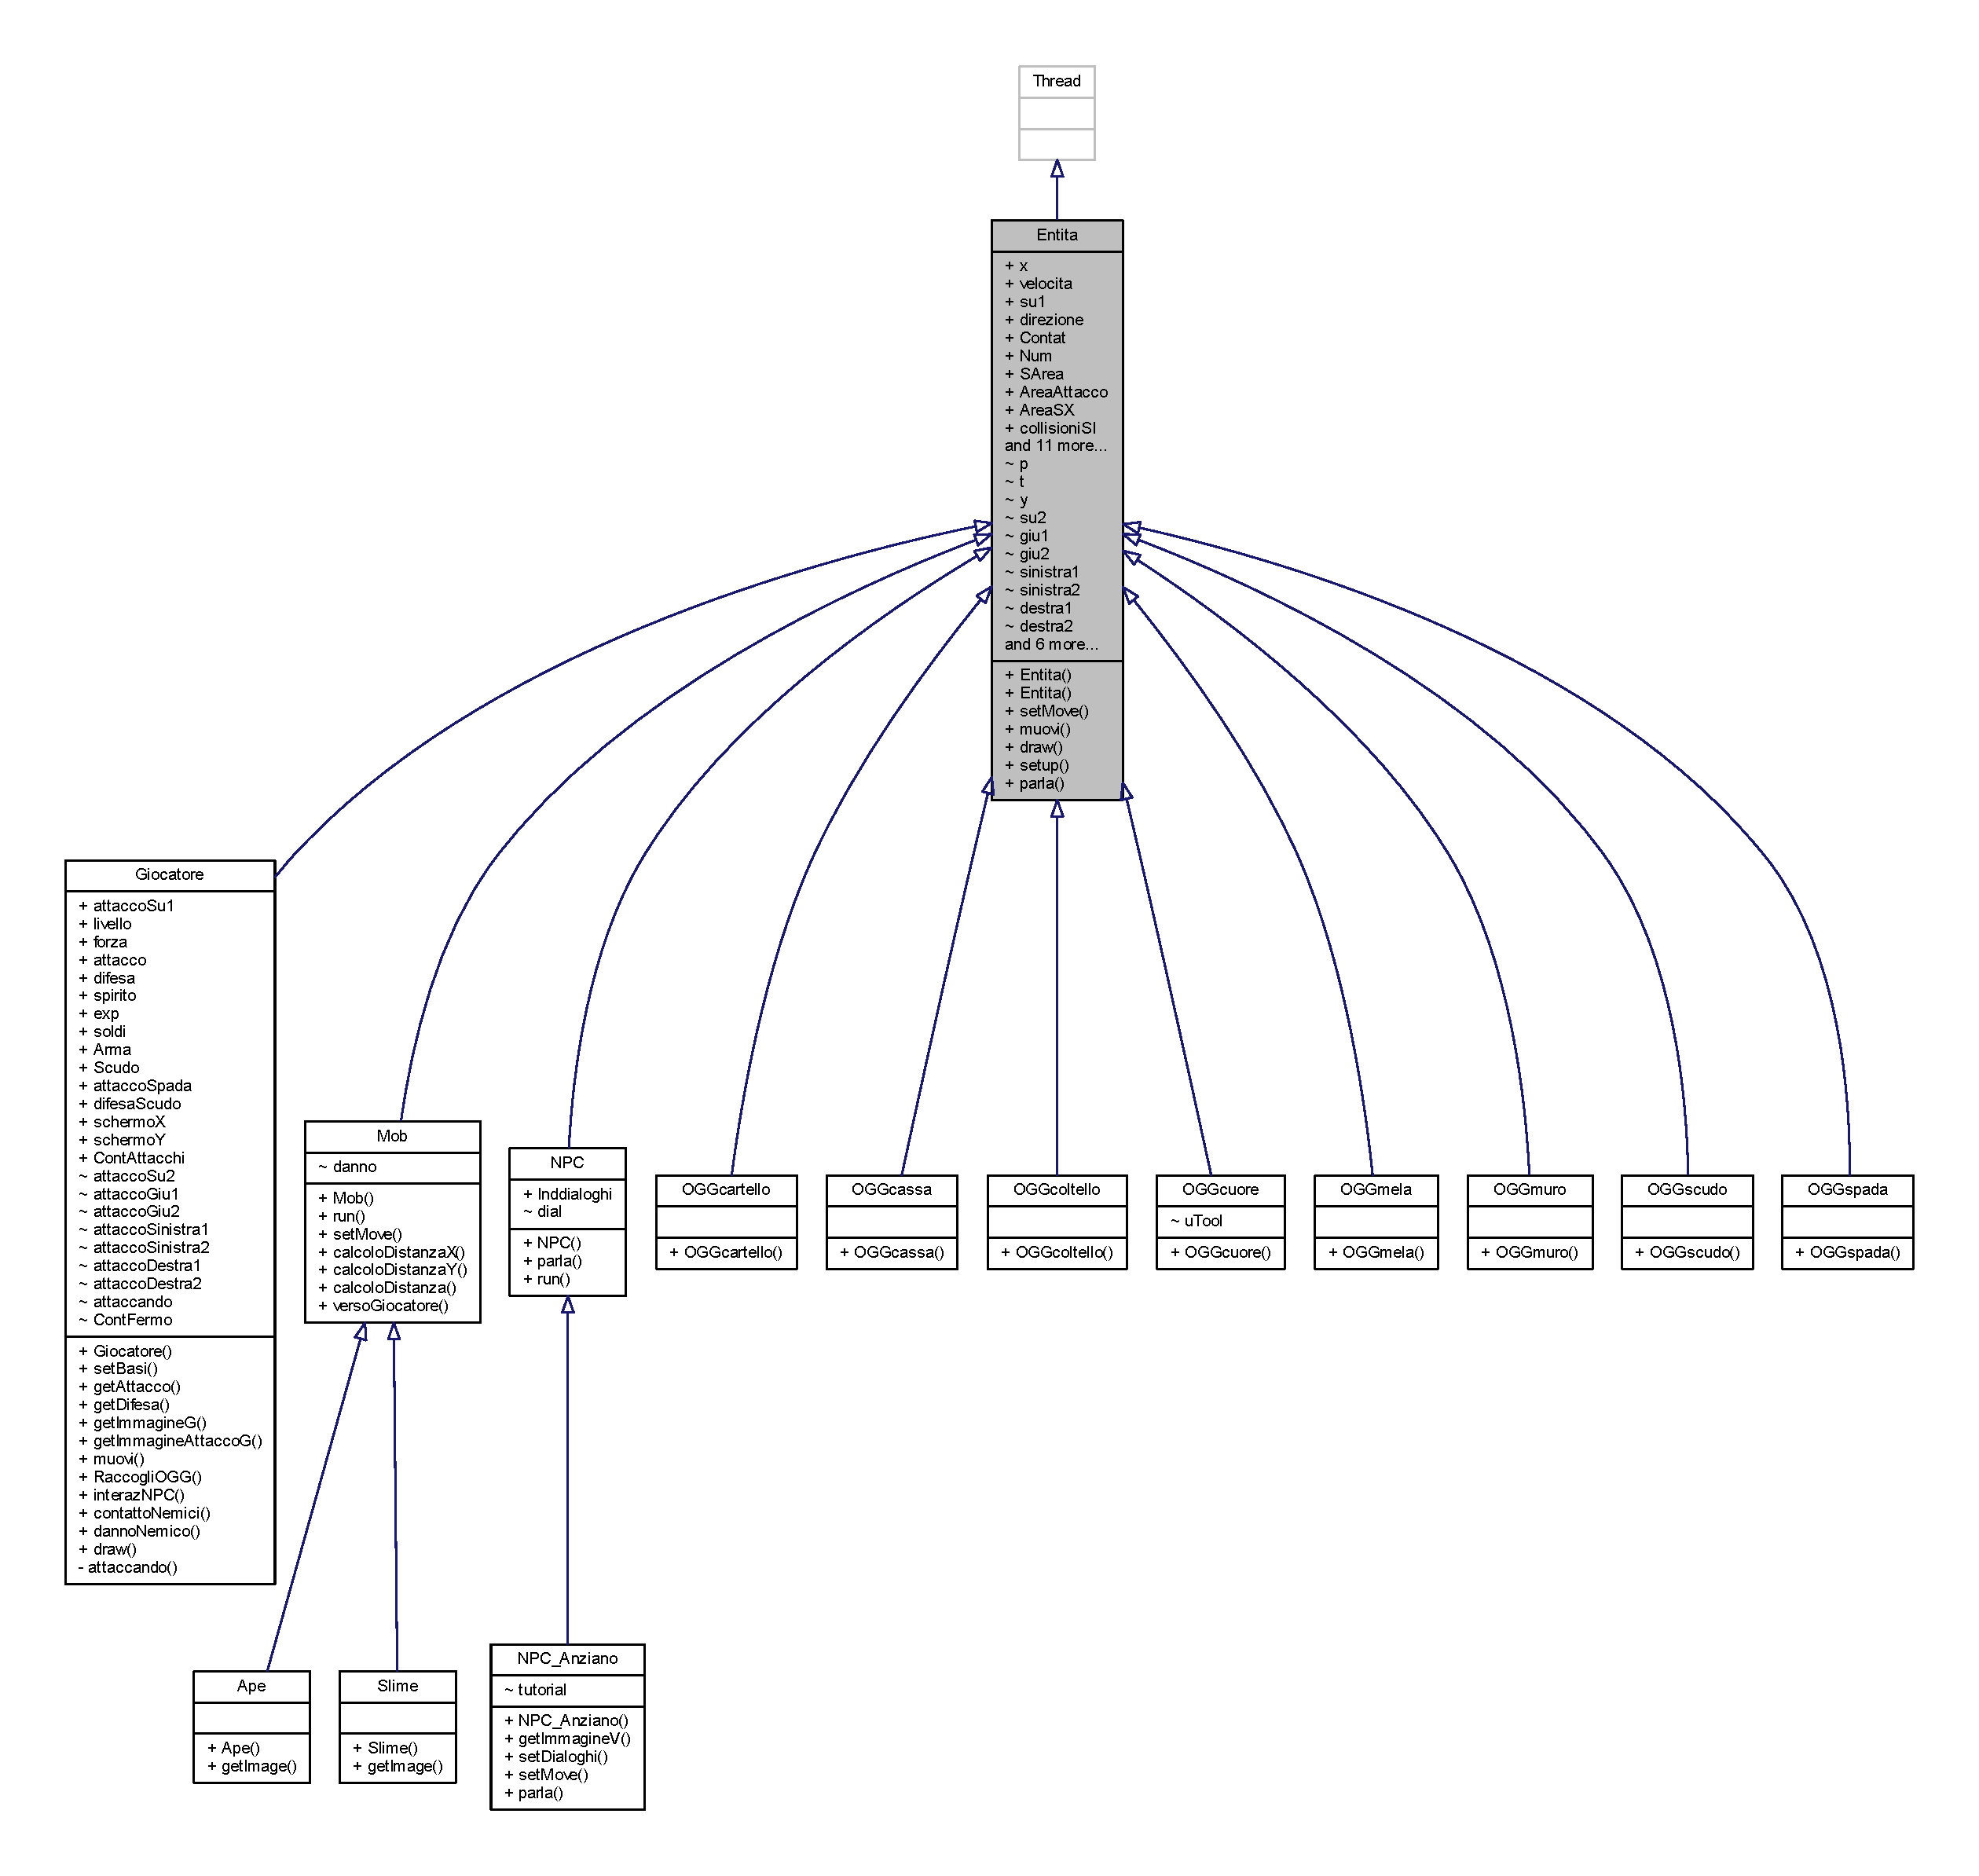
\includegraphics[width=350pt]{class_entita_1_1_entita__inherit__graph}
\end{center}
\end{figure}


Collaboration diagram for Entita\+:
\nopagebreak
\begin{figure}[H]
\begin{center}
\leavevmode
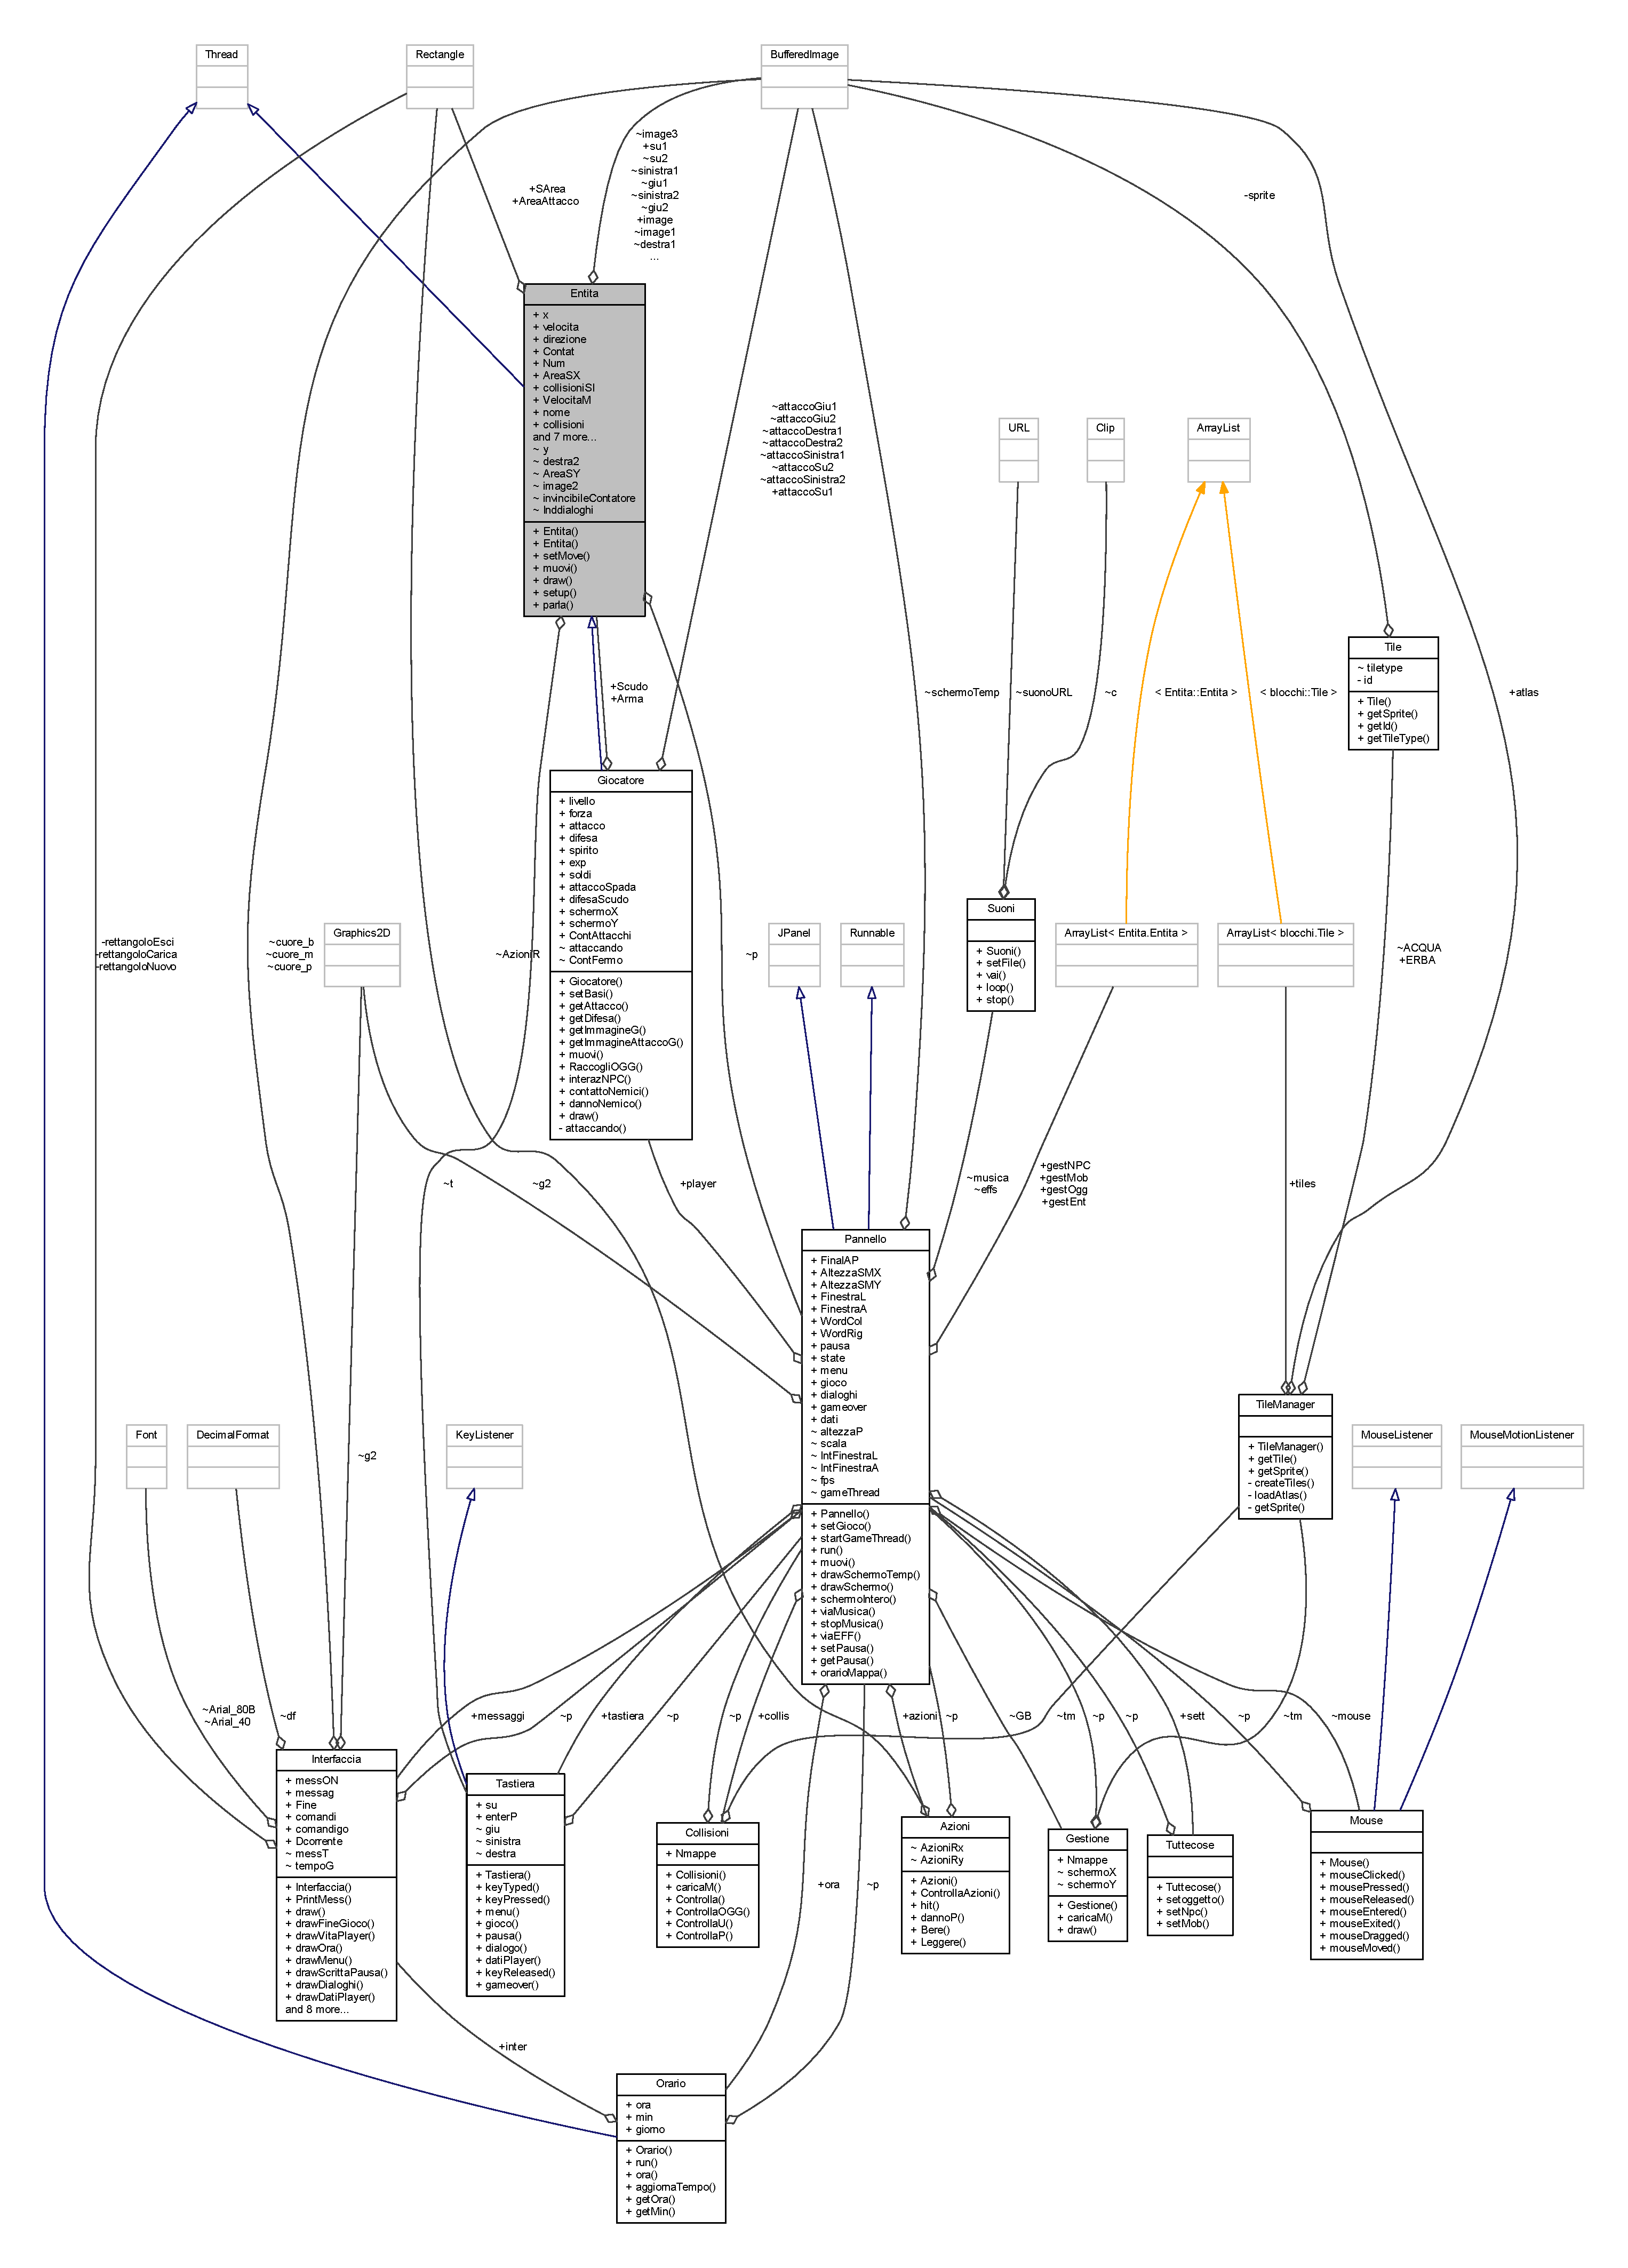
\includegraphics[width=350pt]{class_entita_1_1_entita__coll__graph}
\end{center}
\end{figure}
\subsection*{Public Member Functions}
\begin{DoxyCompactItemize}
\item 
\hyperlink{class_entita_1_1_entita_a2080d433e5b9b6ce5c9f0b9ec426e6fb}{Entita} (\hyperlink{classa_1_1survival_1_1game_1_1_pannello}{Pannello} p)
\item 
\hyperlink{class_entita_1_1_entita_a6984a7f67889d66d0b6e3627ff46b289}{Entita} (\hyperlink{classa_1_1survival_1_1game_1_1_pannello}{Pannello} p, \hyperlink{classa_1_1survival_1_1game_1_1_tastiera}{Tastiera} t)
\item 
void \hyperlink{class_entita_1_1_entita_a447f807a76b7ea97a78cb76241fe8bc8}{set\+Move} ()
\item 
void \hyperlink{class_entita_1_1_entita_a1fe2f184b3cc7345c6a0f08d183a1d0b}{muovi} ()
\begin{DoxyCompactList}\small\item\em metodo per gestire collisioni con i vari npc \end{DoxyCompactList}\item 
void \hyperlink{class_entita_1_1_entita_ae8c972c0fb4fcbc09c2219dd32cbd053}{draw} (Graphics2D g2)
\begin{DoxyCompactList}\small\item\em Metodo per printare le immagini dei mob in base alla direzione in cui puntano. \end{DoxyCompactList}\item 
Buffered\+Image \hyperlink{class_entita_1_1_entita_a2f9ef9abd43cd7e34cd446aef3f499ab}{setup} (String Nimmagine, int l, int a)
\begin{DoxyCompactList}\small\item\em Metodo per settare la grandezza dei vari tile. \end{DoxyCompactList}\item 
void \hyperlink{class_entita_1_1_entita_a8310c90e226ac9bc11547a3adb9cd0f3}{parla} ()
\end{DoxyCompactItemize}
\subsection*{Public Attributes}
\begin{DoxyCompactItemize}
\item 
int \hyperlink{class_entita_1_1_entita_a6150e0515f7202e2fb518f7206ed97dc}{x}
\item 
int \hyperlink{class_entita_1_1_entita_a40cd1c33d6ccf3a0571a5c5aa3c51a25}{velocita}
\item 
Buffered\+Image \hyperlink{class_entita_1_1_entita_a6e18c56eb6db900f07db511b10b4f075}{su1}
\item 
String \hyperlink{class_entita_1_1_entita_a5bda37a4dbca5f275a41dd383b905277}{direzione} =\char`\"{}giu\char`\"{}
\item 
int \hyperlink{class_entita_1_1_entita_a679c3f7220a014c0a3b78e6023747964}{Contat} =0
\item 
int \hyperlink{class_entita_1_1_entita_a558051bc0b213b418d65f58e4ad9a311}{Num} =1
\item 
Rectangle \hyperlink{class_entita_1_1_entita_abc4c4a84c9edea554a8b72a7d929e664}{S\+Area} =new Rectangle(0,0,48,48)
\item 
Rectangle \hyperlink{class_entita_1_1_entita_aee10046794f54deadcafb19e0494a719}{Area\+Attacco} =new Rectangle(0,0,0,0)
\item 
int \hyperlink{class_entita_1_1_entita_a2d5e9de91cc316910aafdea3973089d8}{Area\+SX}
\item 
boolean \hyperlink{class_entita_1_1_entita_a8253afab60c658fa3427e97e63e8d4ea}{collisioni\+SI} =false
\item 
int \hyperlink{class_entita_1_1_entita_a90a894e061963f9de7d3619983627ccc}{VelocitaM} =0
\item 
Buffered\+Image \hyperlink{class_entita_1_1_entita_a45e94f786577439d02e4f16aefa96717}{image}
\item 
String \hyperlink{class_entita_1_1_entita_a4cfff30ec02286864b995e013b6c2a41}{nome}
\item 
boolean \hyperlink{class_entita_1_1_entita_a8ba457fa7d76f9e2b54085588aced39f}{collisioni} = true
\item 
boolean \hyperlink{class_entita_1_1_entita_afb759606adf5eb47c3e8b17e32968115}{invincibile} =false
\item 
int \hyperlink{class_entita_1_1_entita_a6775e052c6cf2cbafd50a83d1e4b6fc3}{sprite\+Counter} =0
\item 
int \hyperlink{class_entita_1_1_entita_ac765329451135abec74c45e1897abf26}{type}
\item 
int \hyperlink{class_entita_1_1_entita_adf6e8908b656fe5199ca043083e48615}{Vita\+Max}
\item 
int \hyperlink{class_entita_1_1_entita_aa68a3a700682130e7af254a4b325f0cb}{vita}
\item 
int \hyperlink{class_entita_1_1_entita_a955d461d95cf97cd1806f6abc44ce485}{attacco\+Spada}
\item 
int \hyperlink{class_entita_1_1_entita_ad1c7c7fe90e4e2563cac9ed38ccb479d}{difesa\+Scudo}
\end{DoxyCompactItemize}


\subsection{Detailed Description}


Definition at line 24 of file Entita.\+java.



\subsection{Constructor \& Destructor Documentation}
\mbox{\Hypertarget{class_entita_1_1_entita_a2080d433e5b9b6ce5c9f0b9ec426e6fb}\label{class_entita_1_1_entita_a2080d433e5b9b6ce5c9f0b9ec426e6fb}} 
\index{Entita\+::\+Entita@{Entita\+::\+Entita}!Entita@{Entita}}
\index{Entita@{Entita}!Entita\+::\+Entita@{Entita\+::\+Entita}}
\subsubsection{\texorpdfstring{Entita()}{Entita()}\hspace{0.1cm}{\footnotesize\ttfamily [1/2]}}
{\footnotesize\ttfamily \hyperlink{class_entita_1_1_entita}{Entita} (\begin{DoxyParamCaption}\item[{\hyperlink{classa_1_1survival_1_1game_1_1_pannello}{Pannello}}]{p }\end{DoxyParamCaption})}



Definition at line 72 of file Entita.\+java.

\mbox{\Hypertarget{class_entita_1_1_entita_a6984a7f67889d66d0b6e3627ff46b289}\label{class_entita_1_1_entita_a6984a7f67889d66d0b6e3627ff46b289}} 
\index{Entita\+::\+Entita@{Entita\+::\+Entita}!Entita@{Entita}}
\index{Entita@{Entita}!Entita\+::\+Entita@{Entita\+::\+Entita}}
\subsubsection{\texorpdfstring{Entita()}{Entita()}\hspace{0.1cm}{\footnotesize\ttfamily [2/2]}}
{\footnotesize\ttfamily \hyperlink{class_entita_1_1_entita}{Entita} (\begin{DoxyParamCaption}\item[{\hyperlink{classa_1_1survival_1_1game_1_1_pannello}{Pannello}}]{p,  }\item[{\hyperlink{classa_1_1survival_1_1game_1_1_tastiera}{Tastiera}}]{t }\end{DoxyParamCaption})}



Definition at line 76 of file Entita.\+java.



\subsection{Member Function Documentation}
\mbox{\Hypertarget{class_entita_1_1_entita_ae8c972c0fb4fcbc09c2219dd32cbd053}\label{class_entita_1_1_entita_ae8c972c0fb4fcbc09c2219dd32cbd053}} 
\index{Entita\+::\+Entita@{Entita\+::\+Entita}!draw@{draw}}
\index{draw@{draw}!Entita\+::\+Entita@{Entita\+::\+Entita}}
\subsubsection{\texorpdfstring{draw()}{draw()}}
{\footnotesize\ttfamily void draw (\begin{DoxyParamCaption}\item[{Graphics2D}]{g2 }\end{DoxyParamCaption})}



Metodo per printare le immagini dei mob in base alla direzione in cui puntano. 


\begin{DoxyParams}{Parameters}
{\em g2} & \\
\hline
\end{DoxyParams}


Definition at line 137 of file Entita.\+java.

\mbox{\Hypertarget{class_entita_1_1_entita_a1fe2f184b3cc7345c6a0f08d183a1d0b}\label{class_entita_1_1_entita_a1fe2f184b3cc7345c6a0f08d183a1d0b}} 
\index{Entita\+::\+Entita@{Entita\+::\+Entita}!muovi@{muovi}}
\index{muovi@{muovi}!Entita\+::\+Entita@{Entita\+::\+Entita}}
\subsubsection{\texorpdfstring{muovi()}{muovi()}}
{\footnotesize\ttfamily void muovi (\begin{DoxyParamCaption}{ }\end{DoxyParamCaption})}



metodo per gestire collisioni con i vari npc 



Definition at line 88 of file Entita.\+java.

Here is the call graph for this function\+:
\nopagebreak
\begin{figure}[H]
\begin{center}
\leavevmode
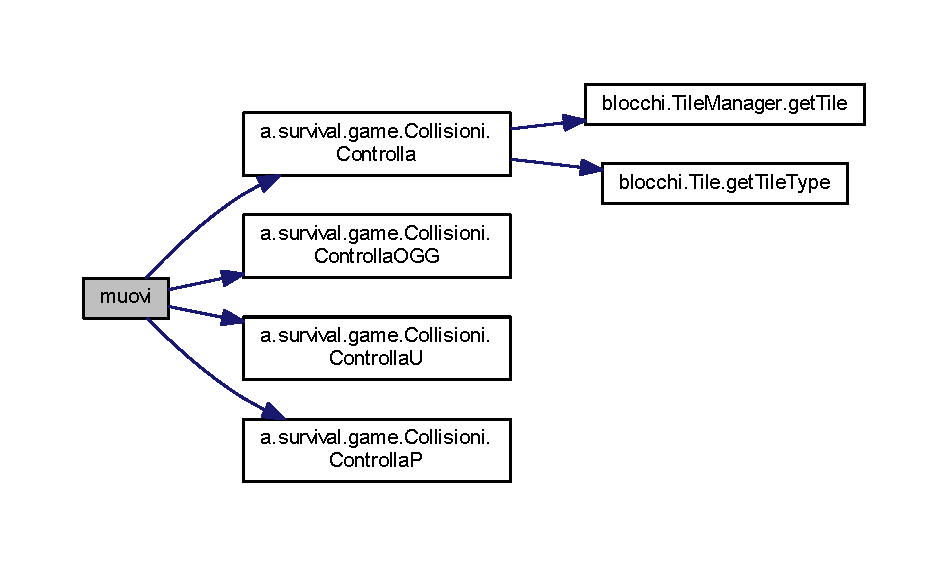
\includegraphics[width=350pt]{class_entita_1_1_entita_a1fe2f184b3cc7345c6a0f08d183a1d0b_cgraph}
\end{center}
\end{figure}
Here is the caller graph for this function\+:
\nopagebreak
\begin{figure}[H]
\begin{center}
\leavevmode
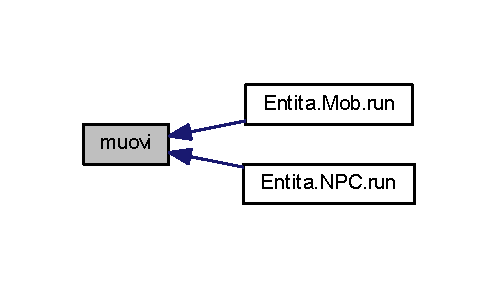
\includegraphics[width=239pt]{class_entita_1_1_entita_a1fe2f184b3cc7345c6a0f08d183a1d0b_icgraph}
\end{center}
\end{figure}
\mbox{\Hypertarget{class_entita_1_1_entita_a8310c90e226ac9bc11547a3adb9cd0f3}\label{class_entita_1_1_entita_a8310c90e226ac9bc11547a3adb9cd0f3}} 
\index{Entita\+::\+Entita@{Entita\+::\+Entita}!parla@{parla}}
\index{parla@{parla}!Entita\+::\+Entita@{Entita\+::\+Entita}}
\subsubsection{\texorpdfstring{parla()}{parla()}}
{\footnotesize\ttfamily void parla (\begin{DoxyParamCaption}{ }\end{DoxyParamCaption})}



Definition at line 196 of file Entita.\+java.

\mbox{\Hypertarget{class_entita_1_1_entita_a447f807a76b7ea97a78cb76241fe8bc8}\label{class_entita_1_1_entita_a447f807a76b7ea97a78cb76241fe8bc8}} 
\index{Entita\+::\+Entita@{Entita\+::\+Entita}!set\+Move@{set\+Move}}
\index{set\+Move@{set\+Move}!Entita\+::\+Entita@{Entita\+::\+Entita}}
\subsubsection{\texorpdfstring{set\+Move()}{setMove()}}
{\footnotesize\ttfamily void set\+Move (\begin{DoxyParamCaption}{ }\end{DoxyParamCaption})}



Definition at line 81 of file Entita.\+java.

\mbox{\Hypertarget{class_entita_1_1_entita_a2f9ef9abd43cd7e34cd446aef3f499ab}\label{class_entita_1_1_entita_a2f9ef9abd43cd7e34cd446aef3f499ab}} 
\index{Entita\+::\+Entita@{Entita\+::\+Entita}!setup@{setup}}
\index{setup@{setup}!Entita\+::\+Entita@{Entita\+::\+Entita}}
\subsubsection{\texorpdfstring{setup()}{setup()}}
{\footnotesize\ttfamily Buffered\+Image setup (\begin{DoxyParamCaption}\item[{String}]{Nimmagine,  }\item[{int}]{l,  }\item[{int}]{a }\end{DoxyParamCaption})}



Metodo per settare la grandezza dei vari tile. 


\begin{DoxyParams}{Parameters}
{\em Nimmagine} & \\
\hline
{\em l} & \\
\hline
{\em a} & \\
\hline
\end{DoxyParams}
\begin{DoxyReturn}{Returns}

\end{DoxyReturn}


Definition at line 183 of file Entita.\+java.

Here is the caller graph for this function\+:
\nopagebreak
\begin{figure}[H]
\begin{center}
\leavevmode
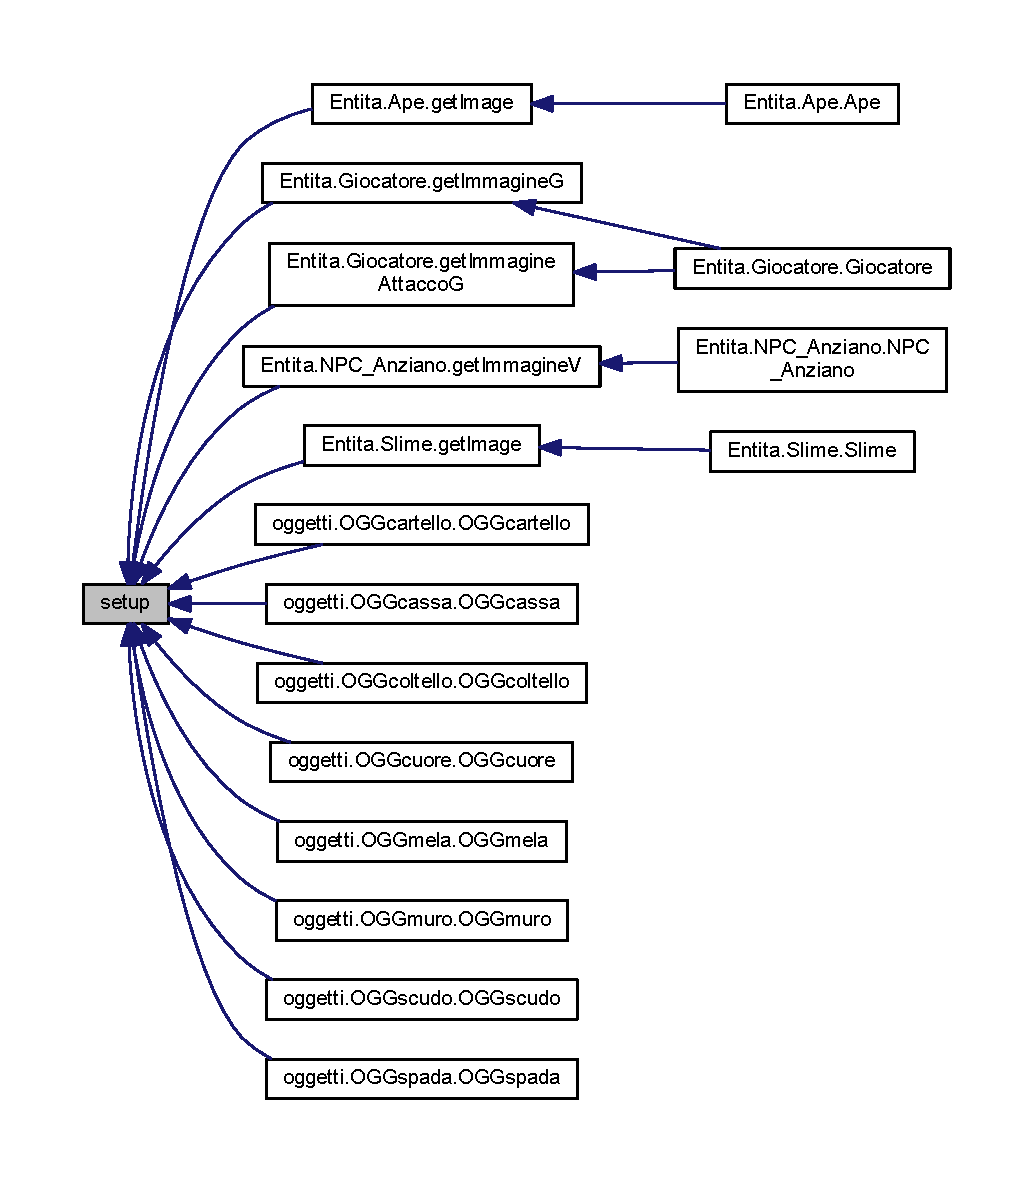
\includegraphics[width=350pt]{class_entita_1_1_entita_a2f9ef9abd43cd7e34cd446aef3f499ab_icgraph}
\end{center}
\end{figure}


\subsection{Member Data Documentation}
\mbox{\Hypertarget{class_entita_1_1_entita_aee10046794f54deadcafb19e0494a719}\label{class_entita_1_1_entita_aee10046794f54deadcafb19e0494a719}} 
\index{Entita\+::\+Entita@{Entita\+::\+Entita}!Area\+Attacco@{Area\+Attacco}}
\index{Area\+Attacco@{Area\+Attacco}!Entita\+::\+Entita@{Entita\+::\+Entita}}
\subsubsection{\texorpdfstring{Area\+Attacco}{AreaAttacco}}
{\footnotesize\ttfamily Rectangle Area\+Attacco =new Rectangle(0,0,0,0)}



Definition at line 42 of file Entita.\+java.

\mbox{\Hypertarget{class_entita_1_1_entita_a2d5e9de91cc316910aafdea3973089d8}\label{class_entita_1_1_entita_a2d5e9de91cc316910aafdea3973089d8}} 
\index{Entita\+::\+Entita@{Entita\+::\+Entita}!Area\+SX@{Area\+SX}}
\index{Area\+SX@{Area\+SX}!Entita\+::\+Entita@{Entita\+::\+Entita}}
\subsubsection{\texorpdfstring{Area\+SX}{AreaSX}}
{\footnotesize\ttfamily int Area\+SX}



Definition at line 44 of file Entita.\+java.

\mbox{\Hypertarget{class_entita_1_1_entita_a955d461d95cf97cd1806f6abc44ce485}\label{class_entita_1_1_entita_a955d461d95cf97cd1806f6abc44ce485}} 
\index{Entita\+::\+Entita@{Entita\+::\+Entita}!attacco\+Spada@{attacco\+Spada}}
\index{attacco\+Spada@{attacco\+Spada}!Entita\+::\+Entita@{Entita\+::\+Entita}}
\subsubsection{\texorpdfstring{attacco\+Spada}{attaccoSpada}}
{\footnotesize\ttfamily int attacco\+Spada}

armi 

Definition at line 66 of file Entita.\+java.

\mbox{\Hypertarget{class_entita_1_1_entita_a8ba457fa7d76f9e2b54085588aced39f}\label{class_entita_1_1_entita_a8ba457fa7d76f9e2b54085588aced39f}} 
\index{Entita\+::\+Entita@{Entita\+::\+Entita}!collisioni@{collisioni}}
\index{collisioni@{collisioni}!Entita\+::\+Entita@{Entita\+::\+Entita}}
\subsubsection{\texorpdfstring{collisioni}{collisioni}}
{\footnotesize\ttfamily boolean collisioni = true}



Definition at line 51 of file Entita.\+java.

\mbox{\Hypertarget{class_entita_1_1_entita_a8253afab60c658fa3427e97e63e8d4ea}\label{class_entita_1_1_entita_a8253afab60c658fa3427e97e63e8d4ea}} 
\index{Entita\+::\+Entita@{Entita\+::\+Entita}!collisioni\+SI@{collisioni\+SI}}
\index{collisioni\+SI@{collisioni\+SI}!Entita\+::\+Entita@{Entita\+::\+Entita}}
\subsubsection{\texorpdfstring{collisioni\+SI}{collisioniSI}}
{\footnotesize\ttfamily boolean collisioni\+SI =false}



Definition at line 45 of file Entita.\+java.

\mbox{\Hypertarget{class_entita_1_1_entita_a679c3f7220a014c0a3b78e6023747964}\label{class_entita_1_1_entita_a679c3f7220a014c0a3b78e6023747964}} 
\index{Entita\+::\+Entita@{Entita\+::\+Entita}!Contat@{Contat}}
\index{Contat@{Contat}!Entita\+::\+Entita@{Entita\+::\+Entita}}
\subsubsection{\texorpdfstring{Contat}{Contat}}
{\footnotesize\ttfamily int Contat =0}



Definition at line 37 of file Entita.\+java.

\mbox{\Hypertarget{class_entita_1_1_entita_ad1c7c7fe90e4e2563cac9ed38ccb479d}\label{class_entita_1_1_entita_ad1c7c7fe90e4e2563cac9ed38ccb479d}} 
\index{Entita\+::\+Entita@{Entita\+::\+Entita}!difesa\+Scudo@{difesa\+Scudo}}
\index{difesa\+Scudo@{difesa\+Scudo}!Entita\+::\+Entita@{Entita\+::\+Entita}}
\subsubsection{\texorpdfstring{difesa\+Scudo}{difesaScudo}}
{\footnotesize\ttfamily int difesa\+Scudo}



Definition at line 67 of file Entita.\+java.

\mbox{\Hypertarget{class_entita_1_1_entita_a5bda37a4dbca5f275a41dd383b905277}\label{class_entita_1_1_entita_a5bda37a4dbca5f275a41dd383b905277}} 
\index{Entita\+::\+Entita@{Entita\+::\+Entita}!direzione@{direzione}}
\index{direzione@{direzione}!Entita\+::\+Entita@{Entita\+::\+Entita}}
\subsubsection{\texorpdfstring{direzione}{direzione}}
{\footnotesize\ttfamily String direzione =\char`\"{}giu\char`\"{}}



Definition at line 35 of file Entita.\+java.

\mbox{\Hypertarget{class_entita_1_1_entita_a45e94f786577439d02e4f16aefa96717}\label{class_entita_1_1_entita_a45e94f786577439d02e4f16aefa96717}} 
\index{Entita\+::\+Entita@{Entita\+::\+Entita}!image@{image}}
\index{image@{image}!Entita\+::\+Entita@{Entita\+::\+Entita}}
\subsubsection{\texorpdfstring{image}{image}}
{\footnotesize\ttfamily Buffered\+Image image}



Definition at line 49 of file Entita.\+java.

\mbox{\Hypertarget{class_entita_1_1_entita_afb759606adf5eb47c3e8b17e32968115}\label{class_entita_1_1_entita_afb759606adf5eb47c3e8b17e32968115}} 
\index{Entita\+::\+Entita@{Entita\+::\+Entita}!invincibile@{invincibile}}
\index{invincibile@{invincibile}!Entita\+::\+Entita@{Entita\+::\+Entita}}
\subsubsection{\texorpdfstring{invincibile}{invincibile}}
{\footnotesize\ttfamily boolean invincibile =false}

set per far diventare invincibile il player dopo aver subito danni 

Definition at line 54 of file Entita.\+java.

\mbox{\Hypertarget{class_entita_1_1_entita_a4cfff30ec02286864b995e013b6c2a41}\label{class_entita_1_1_entita_a4cfff30ec02286864b995e013b6c2a41}} 
\index{Entita\+::\+Entita@{Entita\+::\+Entita}!nome@{nome}}
\index{nome@{nome}!Entita\+::\+Entita@{Entita\+::\+Entita}}
\subsubsection{\texorpdfstring{nome}{nome}}
{\footnotesize\ttfamily String nome}



Definition at line 50 of file Entita.\+java.

\mbox{\Hypertarget{class_entita_1_1_entita_a558051bc0b213b418d65f58e4ad9a311}\label{class_entita_1_1_entita_a558051bc0b213b418d65f58e4ad9a311}} 
\index{Entita\+::\+Entita@{Entita\+::\+Entita}!Num@{Num}}
\index{Num@{Num}!Entita\+::\+Entita@{Entita\+::\+Entita}}
\subsubsection{\texorpdfstring{Num}{Num}}
{\footnotesize\ttfamily int Num =1}



Definition at line 38 of file Entita.\+java.

\mbox{\Hypertarget{class_entita_1_1_entita_abc4c4a84c9edea554a8b72a7d929e664}\label{class_entita_1_1_entita_abc4c4a84c9edea554a8b72a7d929e664}} 
\index{Entita\+::\+Entita@{Entita\+::\+Entita}!S\+Area@{S\+Area}}
\index{S\+Area@{S\+Area}!Entita\+::\+Entita@{Entita\+::\+Entita}}
\subsubsection{\texorpdfstring{S\+Area}{SArea}}
{\footnotesize\ttfamily Rectangle S\+Area =new Rectangle(0,0,48,48)}

set Area per le collisioni 

Definition at line 41 of file Entita.\+java.

\mbox{\Hypertarget{class_entita_1_1_entita_a6775e052c6cf2cbafd50a83d1e4b6fc3}\label{class_entita_1_1_entita_a6775e052c6cf2cbafd50a83d1e4b6fc3}} 
\index{Entita\+::\+Entita@{Entita\+::\+Entita}!sprite\+Counter@{sprite\+Counter}}
\index{sprite\+Counter@{sprite\+Counter}!Entita\+::\+Entita@{Entita\+::\+Entita}}
\subsubsection{\texorpdfstring{sprite\+Counter}{spriteCounter}}
{\footnotesize\ttfamily int sprite\+Counter =0}



Definition at line 56 of file Entita.\+java.

\mbox{\Hypertarget{class_entita_1_1_entita_a6e18c56eb6db900f07db511b10b4f075}\label{class_entita_1_1_entita_a6e18c56eb6db900f07db511b10b4f075}} 
\index{Entita\+::\+Entita@{Entita\+::\+Entita}!su1@{su1}}
\index{su1@{su1}!Entita\+::\+Entita@{Entita\+::\+Entita}}
\subsubsection{\texorpdfstring{su1}{su1}}
{\footnotesize\ttfamily Buffered\+Image su1}

direzione mob 

Definition at line 34 of file Entita.\+java.

\mbox{\Hypertarget{class_entita_1_1_entita_ac765329451135abec74c45e1897abf26}\label{class_entita_1_1_entita_ac765329451135abec74c45e1897abf26}} 
\index{Entita\+::\+Entita@{Entita\+::\+Entita}!type@{type}}
\index{type@{type}!Entita\+::\+Entita@{Entita\+::\+Entita}}
\subsubsection{\texorpdfstring{type}{type}}
{\footnotesize\ttfamily int type}



Definition at line 59 of file Entita.\+java.

\mbox{\Hypertarget{class_entita_1_1_entita_a40cd1c33d6ccf3a0571a5c5aa3c51a25}\label{class_entita_1_1_entita_a40cd1c33d6ccf3a0571a5c5aa3c51a25}} 
\index{Entita\+::\+Entita@{Entita\+::\+Entita}!velocita@{velocita}}
\index{velocita@{velocita}!Entita\+::\+Entita@{Entita\+::\+Entita}}
\subsubsection{\texorpdfstring{velocita}{velocita}}
{\footnotesize\ttfamily int velocita}

velocita dei vari mob 

Definition at line 31 of file Entita.\+java.

\mbox{\Hypertarget{class_entita_1_1_entita_a90a894e061963f9de7d3619983627ccc}\label{class_entita_1_1_entita_a90a894e061963f9de7d3619983627ccc}} 
\index{Entita\+::\+Entita@{Entita\+::\+Entita}!VelocitaM@{VelocitaM}}
\index{VelocitaM@{VelocitaM}!Entita\+::\+Entita@{Entita\+::\+Entita}}
\subsubsection{\texorpdfstring{VelocitaM}{VelocitaM}}
{\footnotesize\ttfamily int VelocitaM =0}



Definition at line 46 of file Entita.\+java.

\mbox{\Hypertarget{class_entita_1_1_entita_aa68a3a700682130e7af254a4b325f0cb}\label{class_entita_1_1_entita_aa68a3a700682130e7af254a4b325f0cb}} 
\index{Entita\+::\+Entita@{Entita\+::\+Entita}!vita@{vita}}
\index{vita@{vita}!Entita\+::\+Entita@{Entita\+::\+Entita}}
\subsubsection{\texorpdfstring{vita}{vita}}
{\footnotesize\ttfamily int vita}



Definition at line 63 of file Entita.\+java.

\mbox{\Hypertarget{class_entita_1_1_entita_adf6e8908b656fe5199ca043083e48615}\label{class_entita_1_1_entita_adf6e8908b656fe5199ca043083e48615}} 
\index{Entita\+::\+Entita@{Entita\+::\+Entita}!Vita\+Max@{Vita\+Max}}
\index{Vita\+Max@{Vita\+Max}!Entita\+::\+Entita@{Entita\+::\+Entita}}
\subsubsection{\texorpdfstring{Vita\+Max}{VitaMax}}
{\footnotesize\ttfamily int Vita\+Max}

vita giocatore 

Definition at line 62 of file Entita.\+java.

\mbox{\Hypertarget{class_entita_1_1_entita_a6150e0515f7202e2fb518f7206ed97dc}\label{class_entita_1_1_entita_a6150e0515f7202e2fb518f7206ed97dc}} 
\index{Entita\+::\+Entita@{Entita\+::\+Entita}!x@{x}}
\index{x@{x}!Entita\+::\+Entita@{Entita\+::\+Entita}}
\subsubsection{\texorpdfstring{x}{x}}
{\footnotesize\ttfamily int x}

x e y mob 

Definition at line 29 of file Entita.\+java.



The documentation for this class was generated from the following file\+:\begin{DoxyCompactItemize}
\item 
src/\+Entita/\hyperlink{_entita_8java}{Entita.\+java}\end{DoxyCompactItemize}

\hypertarget{classblocchi_1_1_gestione}{}\section{Gestione Class Reference}
\label{classblocchi_1_1_gestione}\index{Gestione@{Gestione}}


Collaboration diagram for Gestione\+:
\nopagebreak
\begin{figure}[H]
\begin{center}
\leavevmode
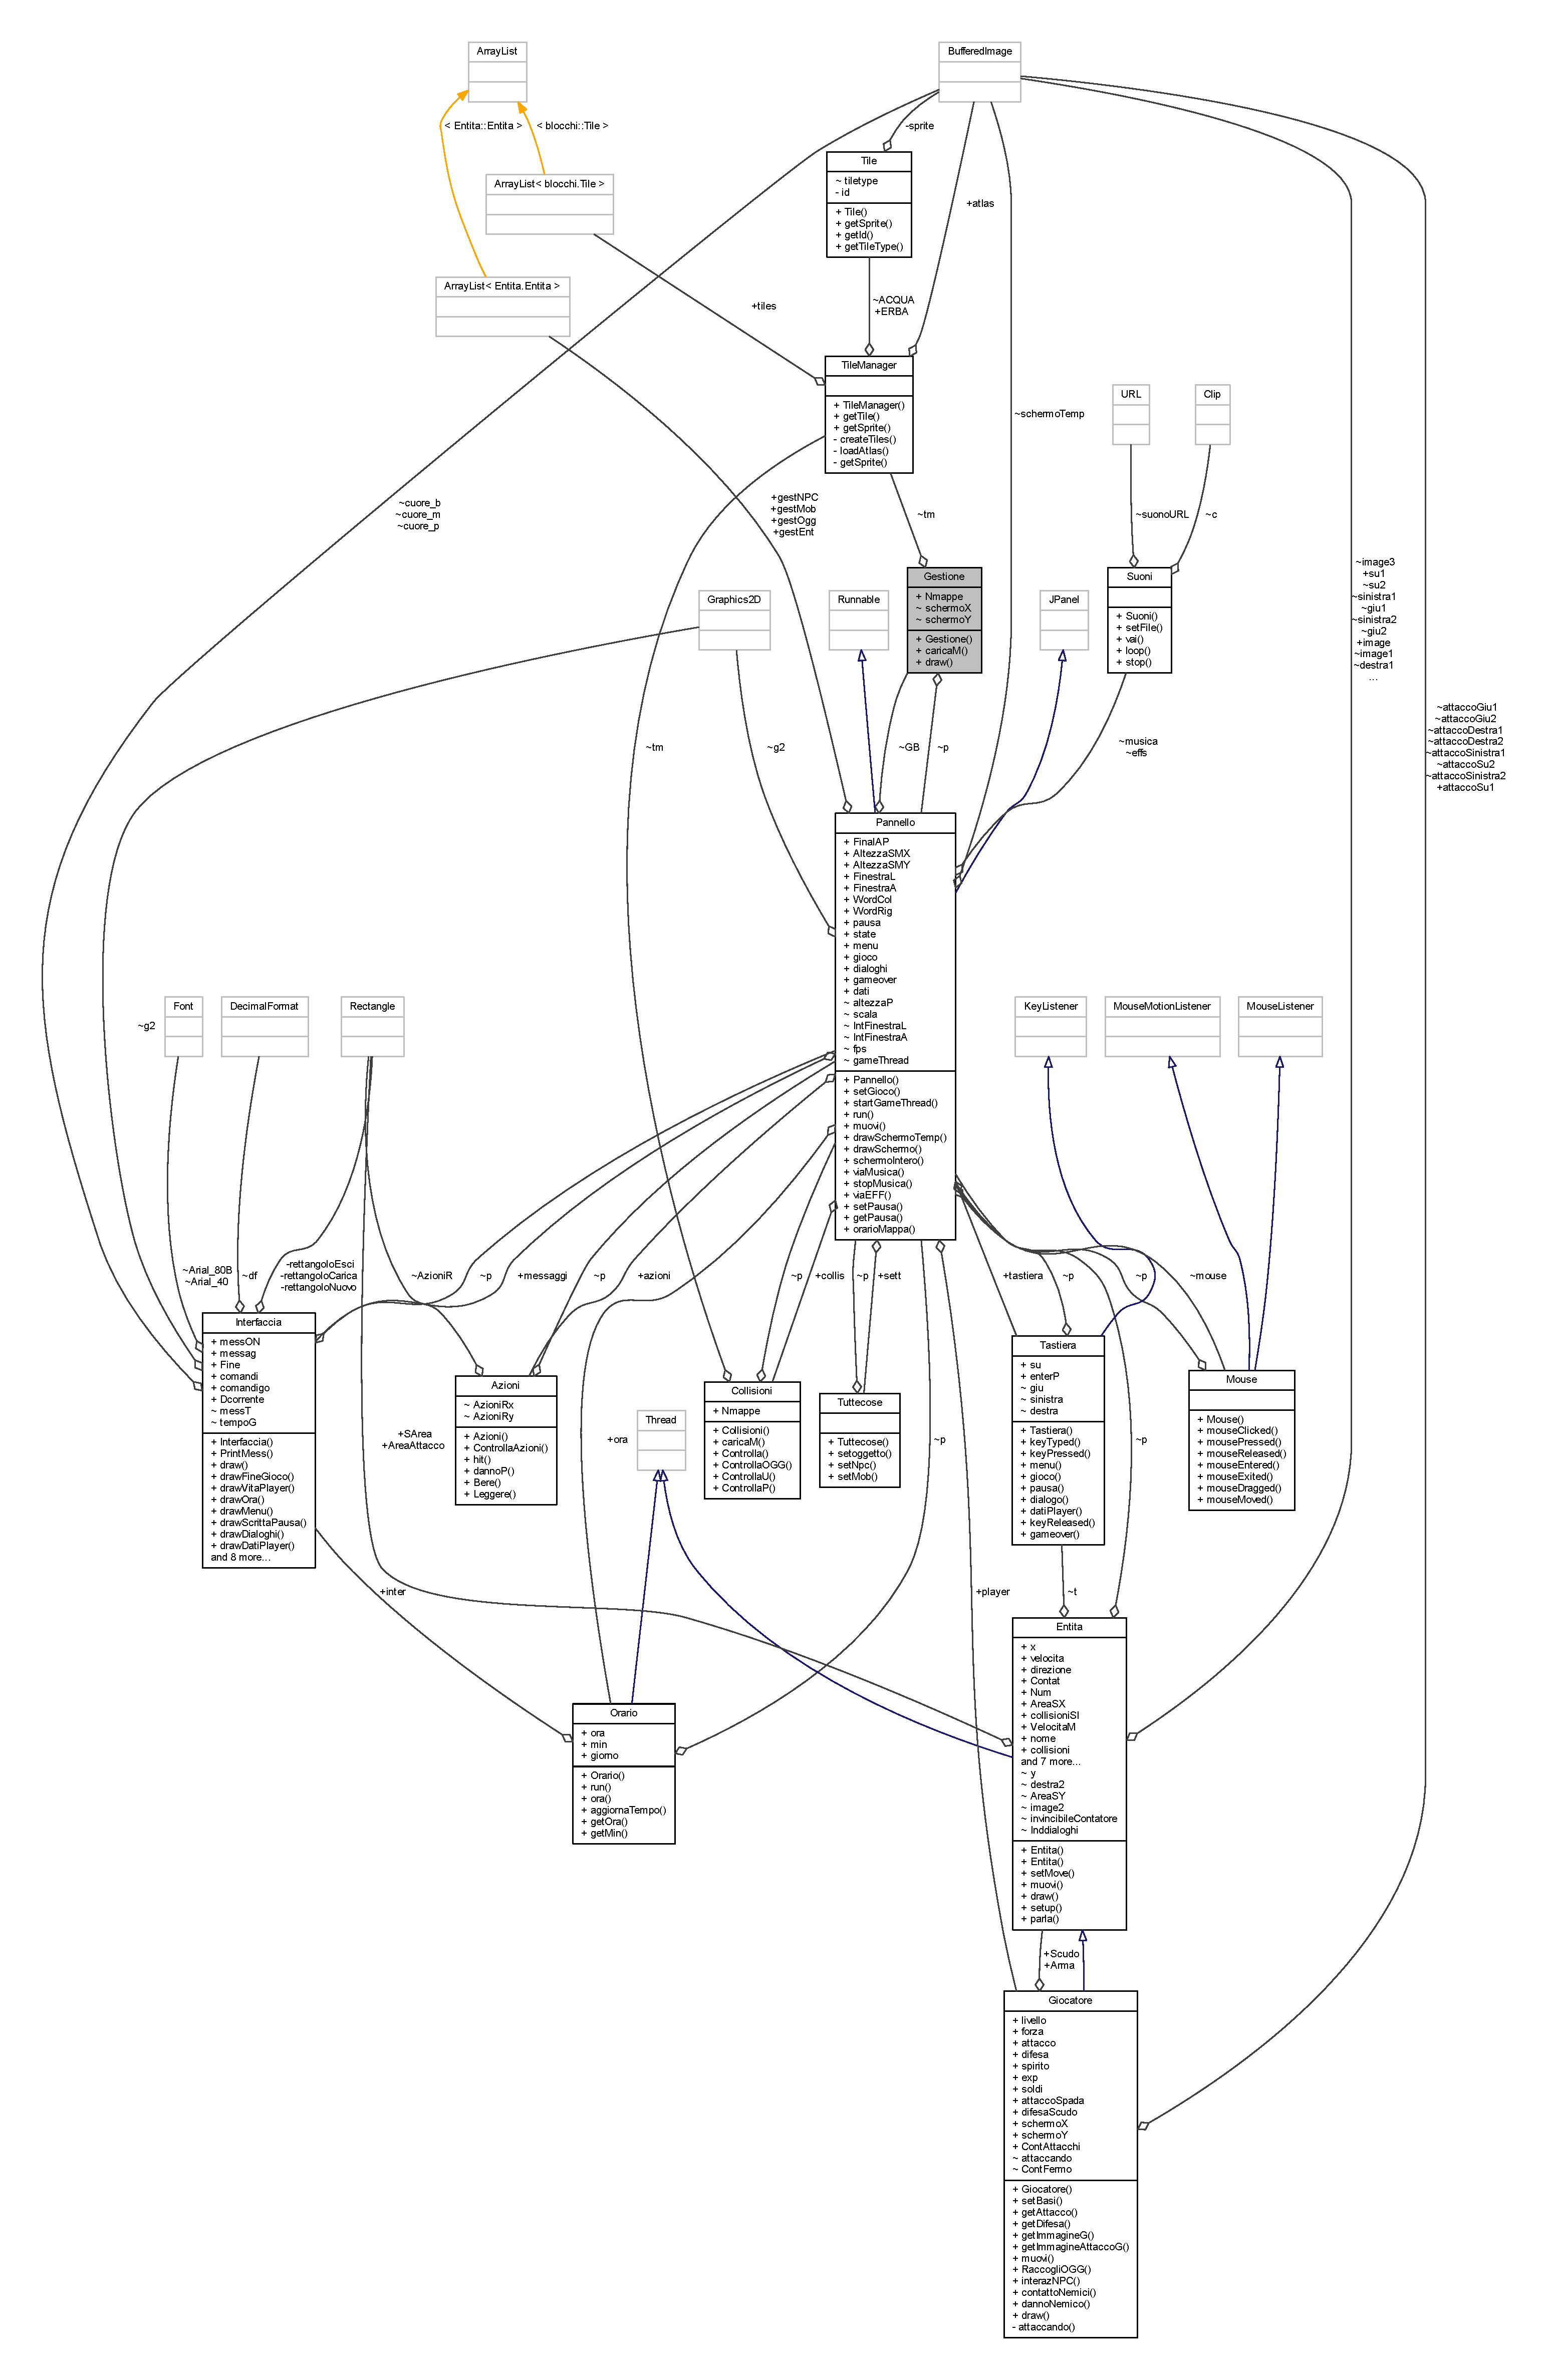
\includegraphics[width=350pt]{classblocchi_1_1_gestione__coll__graph}
\end{center}
\end{figure}
\subsection*{Public Member Functions}
\begin{DoxyCompactItemize}
\item 
\hyperlink{classblocchi_1_1_gestione_a5bc02f9cbad6e4f5c1a061b599a9f5da}{Gestione} (\hyperlink{classa_1_1survival_1_1game_1_1_pannello}{Pannello} p)
\begin{DoxyCompactList}\small\item\em Costruttore parametrico. \end{DoxyCompactList}\item 
void \hyperlink{classblocchi_1_1_gestione_a373d83d9b42d31e72ccc982a3fd85ea9}{caricaM} (String file)
\begin{DoxyCompactList}\small\item\em Metodo per trasformare il txt e i vari numeri in tile. \end{DoxyCompactList}\item 
void \hyperlink{classblocchi_1_1_gestione_ae8c972c0fb4fcbc09c2219dd32cbd053}{draw} (Graphics2D g2)
\begin{DoxyCompactList}\small\item\em Metodo per printare la mappa. \end{DoxyCompactList}\end{DoxyCompactItemize}
\subsection*{Public Attributes}
\begin{DoxyCompactItemize}
\item 
int \hyperlink{classblocchi_1_1_gestione_ac67a253aa050f8b036b79e9613b946e9}{Nmappe} \mbox{[}$\,$\mbox{]}\mbox{[}$\,$\mbox{]}
\end{DoxyCompactItemize}


\subsection{Detailed Description}


Definition at line 19 of file Gestione.\+java.



\subsection{Constructor \& Destructor Documentation}
\mbox{\Hypertarget{classblocchi_1_1_gestione_a5bc02f9cbad6e4f5c1a061b599a9f5da}\label{classblocchi_1_1_gestione_a5bc02f9cbad6e4f5c1a061b599a9f5da}} 
\index{blocchi\+::\+Gestione@{blocchi\+::\+Gestione}!Gestione@{Gestione}}
\index{Gestione@{Gestione}!blocchi\+::\+Gestione@{blocchi\+::\+Gestione}}
\subsubsection{\texorpdfstring{Gestione()}{Gestione()}}
{\footnotesize\ttfamily \hyperlink{classblocchi_1_1_gestione}{Gestione} (\begin{DoxyParamCaption}\item[{\hyperlink{classa_1_1survival_1_1game_1_1_pannello}{Pannello}}]{p }\end{DoxyParamCaption})}



Costruttore parametrico. 


\begin{DoxyParams}{Parameters}
{\em p} & \\
\hline
\end{DoxyParams}
Richiamo il metodo caricaM e gli passo il txt dove prendere la mappa 

Definition at line 34 of file Gestione.\+java.

Here is the call graph for this function\+:
\nopagebreak
\begin{figure}[H]
\begin{center}
\leavevmode
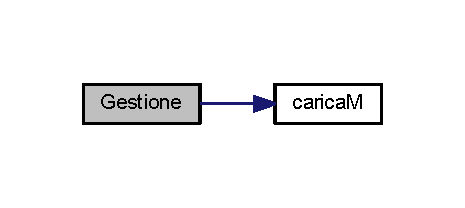
\includegraphics[width=223pt]{classblocchi_1_1_gestione_a5bc02f9cbad6e4f5c1a061b599a9f5da_cgraph}
\end{center}
\end{figure}


\subsection{Member Function Documentation}
\mbox{\Hypertarget{classblocchi_1_1_gestione_a373d83d9b42d31e72ccc982a3fd85ea9}\label{classblocchi_1_1_gestione_a373d83d9b42d31e72ccc982a3fd85ea9}} 
\index{blocchi\+::\+Gestione@{blocchi\+::\+Gestione}!caricaM@{caricaM}}
\index{caricaM@{caricaM}!blocchi\+::\+Gestione@{blocchi\+::\+Gestione}}
\subsubsection{\texorpdfstring{carica\+M()}{caricaM()}}
{\footnotesize\ttfamily void caricaM (\begin{DoxyParamCaption}\item[{String}]{file }\end{DoxyParamCaption})}



Metodo per trasformare il txt e i vari numeri in tile. 


\begin{DoxyParams}{Parameters}
{\em file} & \\
\hline
\end{DoxyParams}


Definition at line 53 of file Gestione.\+java.

Here is the caller graph for this function\+:
\nopagebreak
\begin{figure}[H]
\begin{center}
\leavevmode
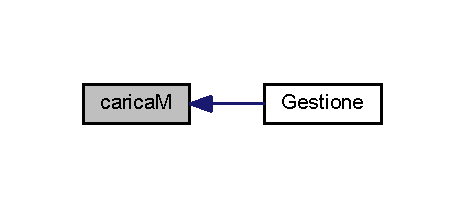
\includegraphics[width=223pt]{classblocchi_1_1_gestione_a373d83d9b42d31e72ccc982a3fd85ea9_icgraph}
\end{center}
\end{figure}
\mbox{\Hypertarget{classblocchi_1_1_gestione_ae8c972c0fb4fcbc09c2219dd32cbd053}\label{classblocchi_1_1_gestione_ae8c972c0fb4fcbc09c2219dd32cbd053}} 
\index{blocchi\+::\+Gestione@{blocchi\+::\+Gestione}!draw@{draw}}
\index{draw@{draw}!blocchi\+::\+Gestione@{blocchi\+::\+Gestione}}
\subsubsection{\texorpdfstring{draw()}{draw()}}
{\footnotesize\ttfamily void draw (\begin{DoxyParamCaption}\item[{Graphics2D}]{g2 }\end{DoxyParamCaption})}



Metodo per printare la mappa. 


\begin{DoxyParams}{Parameters}
{\em g2} & \\
\hline
\end{DoxyParams}


Definition at line 83 of file Gestione.\+java.

Here is the call graph for this function\+:
\nopagebreak
\begin{figure}[H]
\begin{center}
\leavevmode
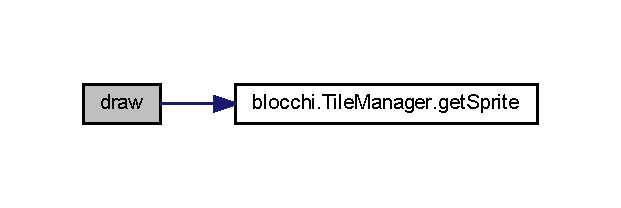
\includegraphics[width=298pt]{classblocchi_1_1_gestione_ae8c972c0fb4fcbc09c2219dd32cbd053_cgraph}
\end{center}
\end{figure}
Here is the caller graph for this function\+:
\nopagebreak
\begin{figure}[H]
\begin{center}
\leavevmode
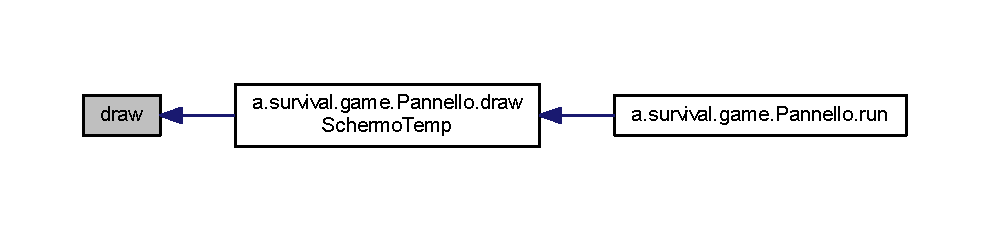
\includegraphics[width=350pt]{classblocchi_1_1_gestione_ae8c972c0fb4fcbc09c2219dd32cbd053_icgraph}
\end{center}
\end{figure}


\subsection{Member Data Documentation}
\mbox{\Hypertarget{classblocchi_1_1_gestione_ac67a253aa050f8b036b79e9613b946e9}\label{classblocchi_1_1_gestione_ac67a253aa050f8b036b79e9613b946e9}} 
\index{blocchi\+::\+Gestione@{blocchi\+::\+Gestione}!Nmappe@{Nmappe}}
\index{Nmappe@{Nmappe}!blocchi\+::\+Gestione@{blocchi\+::\+Gestione}}
\subsubsection{\texorpdfstring{Nmappe}{Nmappe}}
{\footnotesize\ttfamily int Nmappe\mbox{[}$\,$\mbox{]}\mbox{[}$\,$\mbox{]}}

matrice per settare numero tile della mappa 

Definition at line 22 of file Gestione.\+java.



The documentation for this class was generated from the following file\+:\begin{DoxyCompactItemize}
\item 
src/blocchi/\hyperlink{_gestione_8java}{Gestione.\+java}\end{DoxyCompactItemize}

\hypertarget{class_entita_1_1_giocatore}{}\section{Giocatore Class Reference}
\label{class_entita_1_1_giocatore}\index{Giocatore@{Giocatore}}


Classe con extends \hyperlink{class_entita_1_1_entita}{Entita}.  




Inheritance diagram for Giocatore\+:
\nopagebreak
\begin{figure}[H]
\begin{center}
\leavevmode
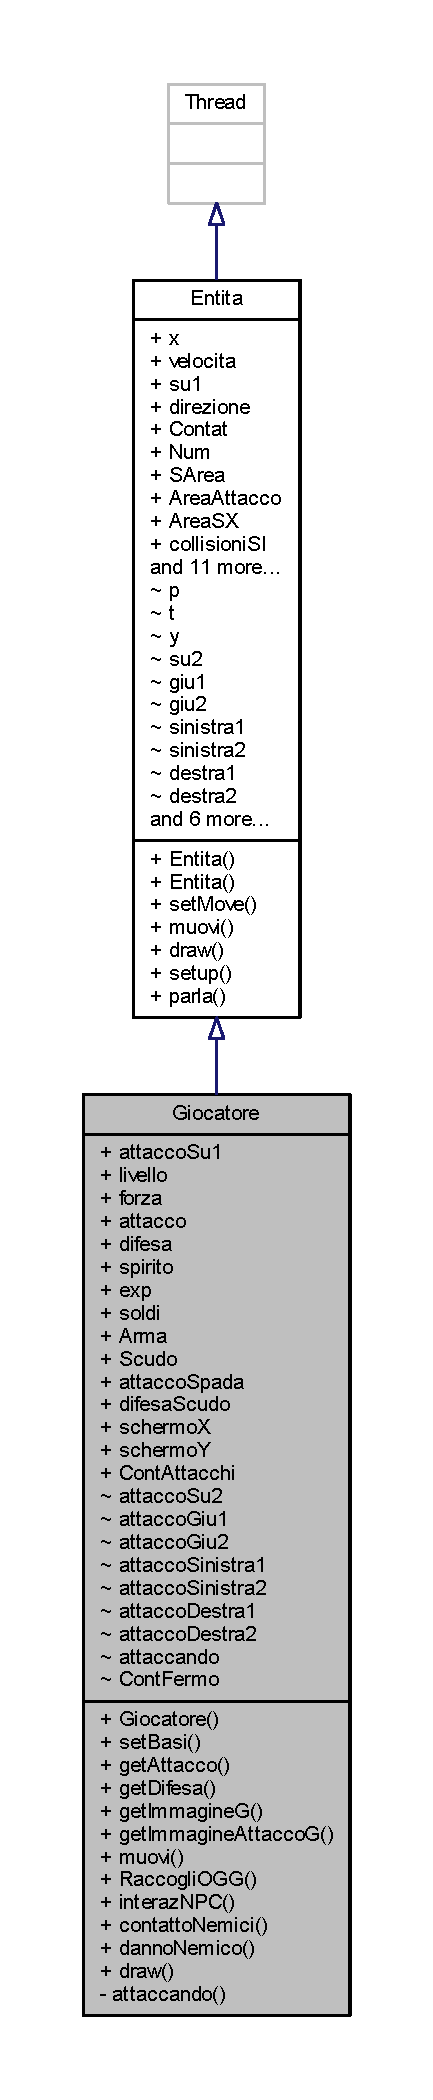
\includegraphics[height=550pt]{class_entita_1_1_giocatore__inherit__graph}
\end{center}
\end{figure}


Collaboration diagram for Giocatore\+:
\nopagebreak
\begin{figure}[H]
\begin{center}
\leavevmode
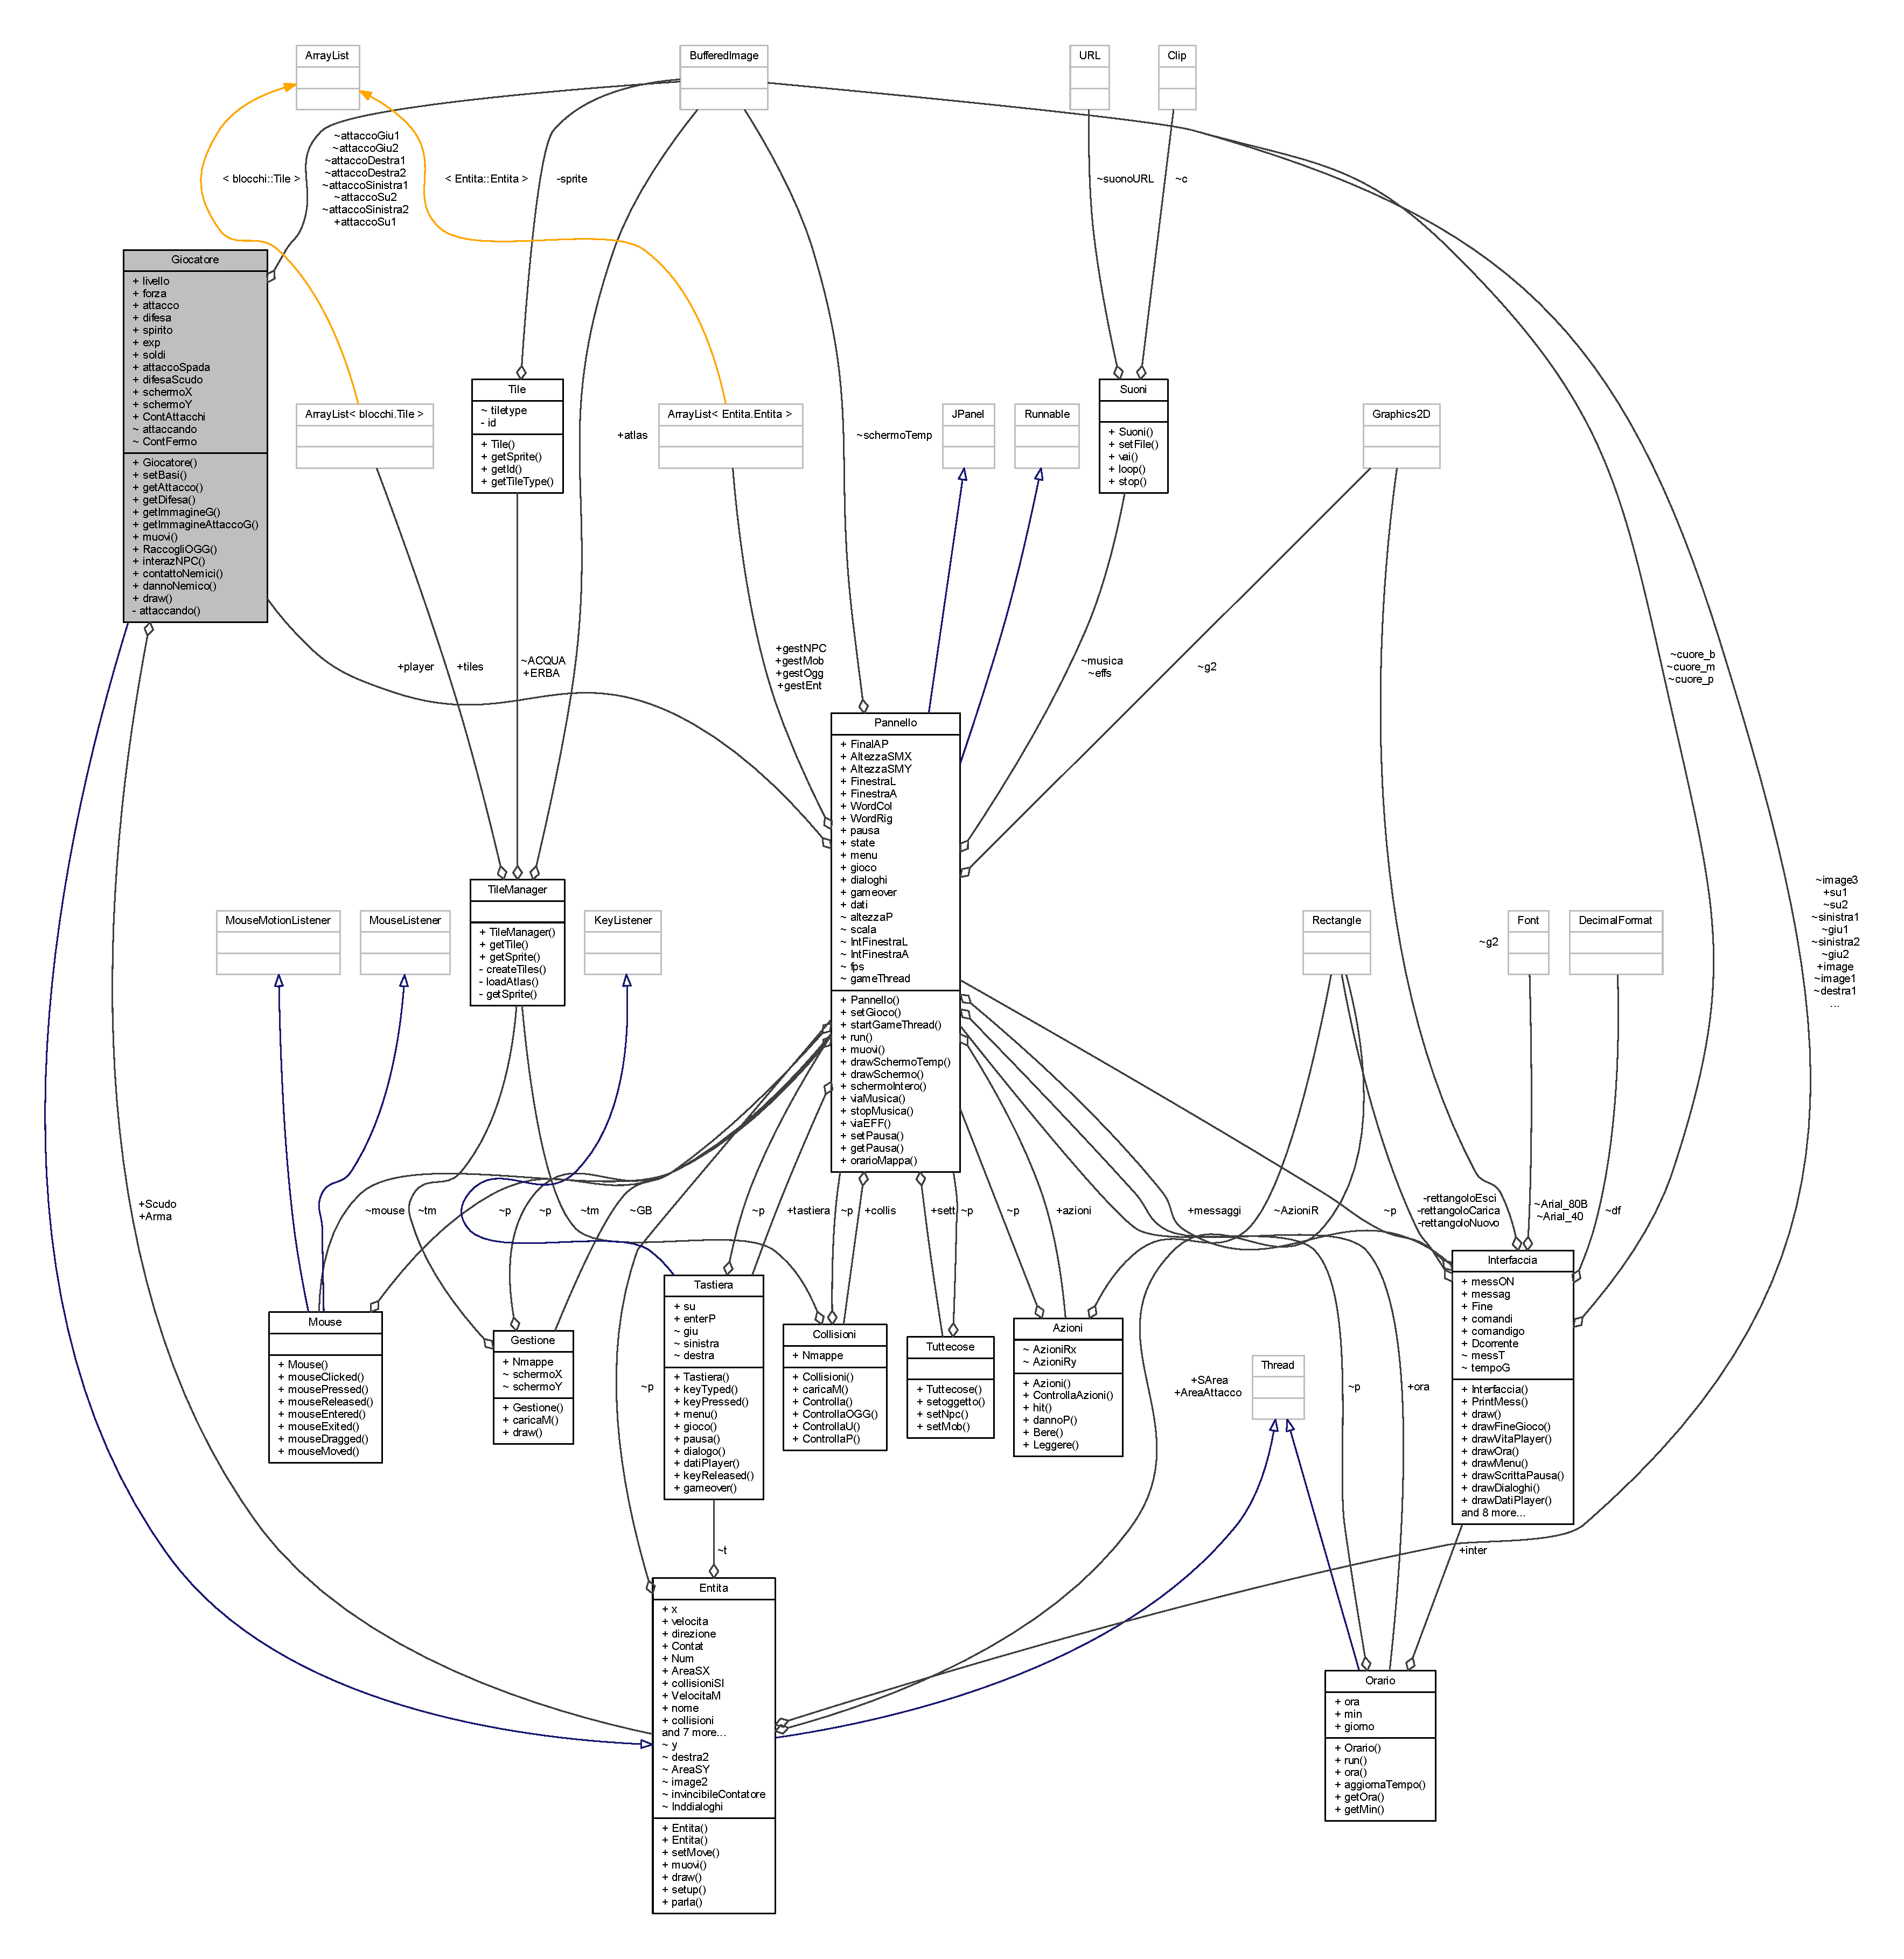
\includegraphics[width=350pt]{class_entita_1_1_giocatore__coll__graph}
\end{center}
\end{figure}
\subsection*{Public Member Functions}
\begin{DoxyCompactItemize}
\item 
\hyperlink{class_entita_1_1_giocatore_ab9baa50cd99d9d2e399e9e3ad53159c6}{Giocatore} (\hyperlink{classa_1_1survival_1_1game_1_1_pannello}{Pannello} p, \hyperlink{classa_1_1survival_1_1game_1_1_tastiera}{Tastiera} t)
\begin{DoxyCompactList}\small\item\em Metodo per caricare immagine del giocatore nel gioco. \end{DoxyCompactList}\item 
void \hyperlink{class_entita_1_1_giocatore_a38a75be5807f155ff640bfa73518421d}{set\+Basi} ()
\begin{DoxyCompactList}\small\item\em Metodo per settare i valori base del giocatore. \end{DoxyCompactList}\item 
int \hyperlink{class_entita_1_1_giocatore_aafeab2e7e3b0e536c594b5aef8c31683}{get\+Attacco} ()
\item 
int \hyperlink{class_entita_1_1_giocatore_a5cd7986fb28ad7739710f90e464b1b27}{get\+Difesa} ()
\item 
void \hyperlink{class_entita_1_1_giocatore_abac365540bed82b4025e8e845b779c72}{get\+ImmagineG} ()
\begin{DoxyCompactList}\small\item\em setto le immagini quando cammino \end{DoxyCompactList}\item 
void \hyperlink{class_entita_1_1_giocatore_acc1691c076ed9335796eac421dce845f}{get\+Immagine\+AttaccoG} ()
\begin{DoxyCompactList}\small\item\em setto le immagini quando attacco \end{DoxyCompactList}\item 
void \hyperlink{class_entita_1_1_giocatore_a1fe2f184b3cc7345c6a0f08d183a1d0b}{muovi} ()
\begin{DoxyCompactList}\small\item\em Metodo per far muovere il player e per caricare in base la direzione l\textquotesingle{}immagine giusta. \end{DoxyCompactList}\item 
void \hyperlink{class_entita_1_1_giocatore_a9ba65e7d25928d62218cf14bee3c0273}{Raccogli\+O\+GG} (int i)
\item 
void \hyperlink{class_entita_1_1_giocatore_aaf1d3a52e79be598afe385c91a9f4d0c}{interaz\+N\+PC} (int i)
\item 
void \hyperlink{class_entita_1_1_giocatore_a867fc5532a9f20042ecde7951b83c499}{contatto\+Nemici} (int i)
\item 
void \hyperlink{class_entita_1_1_giocatore_a0814609fcd5c78e217a57e65bb65f7b4}{danno\+Nemico} (int i)
\begin{DoxyCompactList}\small\item\em quando attacco i nemici diventano involnerabili per breve tempo \end{DoxyCompactList}\item 
void \hyperlink{class_entita_1_1_giocatore_ae8c972c0fb4fcbc09c2219dd32cbd053}{draw} (Graphics2D g2)
\begin{DoxyCompactList}\small\item\em Metodo draw per printare sullo schermo tali immagini. \end{DoxyCompactList}\end{DoxyCompactItemize}
\subsection*{Public Attributes}
\begin{DoxyCompactItemize}
\item 
Buffered\+Image \hyperlink{class_entita_1_1_giocatore_a738b89ee909e3e3b2751a2fa9a959813}{attacco\+Su1}
\item 
int \hyperlink{class_entita_1_1_giocatore_a9df9739330535dcec4121b7a25289af6}{livello}
\item 
int \hyperlink{class_entita_1_1_giocatore_a11a8dccab7cd0e8facbe3152140e41b8}{forza}
\item 
int \hyperlink{class_entita_1_1_giocatore_a585c716c79ac39d627dd9719b902a64f}{attacco}
\item 
int \hyperlink{class_entita_1_1_giocatore_afdf43c12f58b193223e199b997834e59}{difesa}
\item 
int \hyperlink{class_entita_1_1_giocatore_a531fc785df2ee9bd58da74a801e766c4}{spirito}
\item 
int \hyperlink{class_entita_1_1_giocatore_a3bb4af16b31e7979f424cf66f1bfa6e2}{exp}
\item 
int \hyperlink{class_entita_1_1_giocatore_a4ab2b490b2927b4d21ee663f63f81bd6}{soldi}
\item 
\hyperlink{class_entita_1_1_entita}{Entita} \hyperlink{class_entita_1_1_giocatore_ade56944373ebbc5f5117b39639e3cef5}{Arma}
\item 
\hyperlink{class_entita_1_1_entita}{Entita} \hyperlink{class_entita_1_1_giocatore_a07e5f7f5db8ac85356757f54f153bb20}{Scudo}
\item 
int \hyperlink{class_entita_1_1_giocatore_a955d461d95cf97cd1806f6abc44ce485}{attacco\+Spada}
\item 
int \hyperlink{class_entita_1_1_giocatore_ad1c7c7fe90e4e2563cac9ed38ccb479d}{difesa\+Scudo}
\item 
final int \hyperlink{class_entita_1_1_giocatore_a446b75d761c1ca3d631eaa61b04298d2}{schermoX}
\item 
final int \hyperlink{class_entita_1_1_giocatore_ada8f80a3f9f6b62953b85f6d05d02c50}{schermoY}
\item 
boolean \hyperlink{class_entita_1_1_giocatore_a0ace2881b0b5e4e097b5f406cb9d173b}{Cont\+Attacchi} = false
\end{DoxyCompactItemize}
\subsection*{Private Member Functions}
\begin{DoxyCompactItemize}
\item 
void \hyperlink{class_entita_1_1_giocatore_af4bcd86c7ccc1775a5fece50849563fe}{attaccando} ()
\begin{DoxyCompactList}\small\item\em Metodo per caricare le immagini quando attacco. \end{DoxyCompactList}\end{DoxyCompactItemize}


\subsection{Detailed Description}
Classe con extends \hyperlink{class_entita_1_1_entita}{Entita}. 

Definition at line 22 of file Giocatore.\+java.



\subsection{Constructor \& Destructor Documentation}
\mbox{\Hypertarget{class_entita_1_1_giocatore_ab9baa50cd99d9d2e399e9e3ad53159c6}\label{class_entita_1_1_giocatore_ab9baa50cd99d9d2e399e9e3ad53159c6}} 
\index{Entita\+::\+Giocatore@{Entita\+::\+Giocatore}!Giocatore@{Giocatore}}
\index{Giocatore@{Giocatore}!Entita\+::\+Giocatore@{Entita\+::\+Giocatore}}
\subsubsection{\texorpdfstring{Giocatore()}{Giocatore()}}
{\footnotesize\ttfamily \hyperlink{class_entita_1_1_giocatore}{Giocatore} (\begin{DoxyParamCaption}\item[{\hyperlink{classa_1_1survival_1_1game_1_1_pannello}{Pannello}}]{p,  }\item[{\hyperlink{classa_1_1survival_1_1game_1_1_tastiera}{Tastiera}}]{t }\end{DoxyParamCaption})}



Metodo per caricare immagine del giocatore nel gioco. 


\begin{DoxyParams}{Parameters}
{\em p} & \\
\hline
{\em t} & \\
\hline
\end{DoxyParams}


Definition at line 56 of file Giocatore.\+java.

Here is the call graph for this function\+:
\nopagebreak
\begin{figure}[H]
\begin{center}
\leavevmode
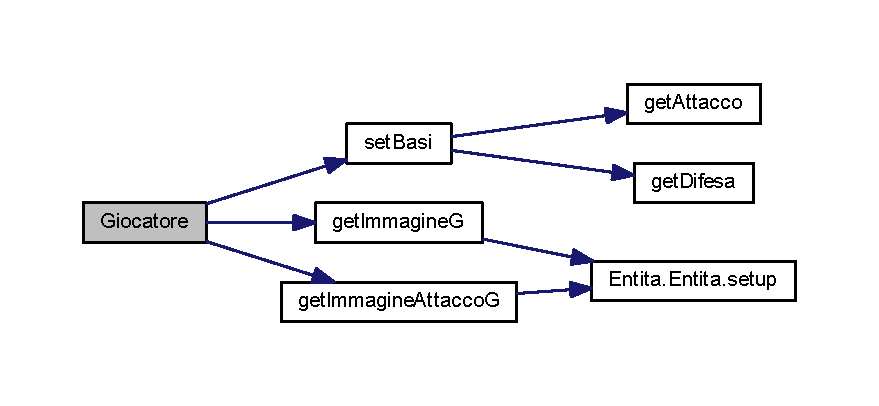
\includegraphics[width=350pt]{class_entita_1_1_giocatore_ab9baa50cd99d9d2e399e9e3ad53159c6_cgraph}
\end{center}
\end{figure}


\subsection{Member Function Documentation}
\mbox{\Hypertarget{class_entita_1_1_giocatore_af4bcd86c7ccc1775a5fece50849563fe}\label{class_entita_1_1_giocatore_af4bcd86c7ccc1775a5fece50849563fe}} 
\index{Entita\+::\+Giocatore@{Entita\+::\+Giocatore}!attaccando@{attaccando}}
\index{attaccando@{attaccando}!Entita\+::\+Giocatore@{Entita\+::\+Giocatore}}
\subsubsection{\texorpdfstring{attaccando()}{attaccando()}}
{\footnotesize\ttfamily void attaccando (\begin{DoxyParamCaption}{ }\end{DoxyParamCaption})\hspace{0.3cm}{\ttfamily [private]}}



Metodo per caricare le immagini quando attacco. 



Definition at line 240 of file Giocatore.\+java.

Here is the call graph for this function\+:
\nopagebreak
\begin{figure}[H]
\begin{center}
\leavevmode
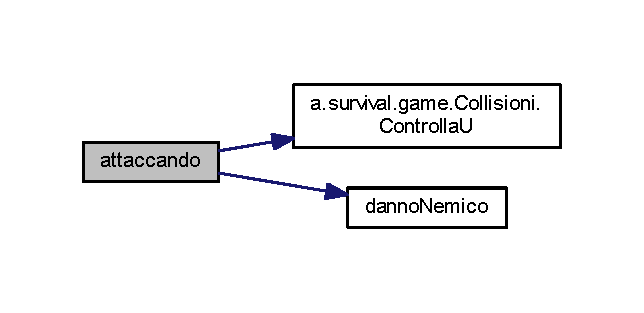
\includegraphics[width=309pt]{class_entita_1_1_giocatore_af4bcd86c7ccc1775a5fece50849563fe_cgraph}
\end{center}
\end{figure}
Here is the caller graph for this function\+:
\nopagebreak
\begin{figure}[H]
\begin{center}
\leavevmode
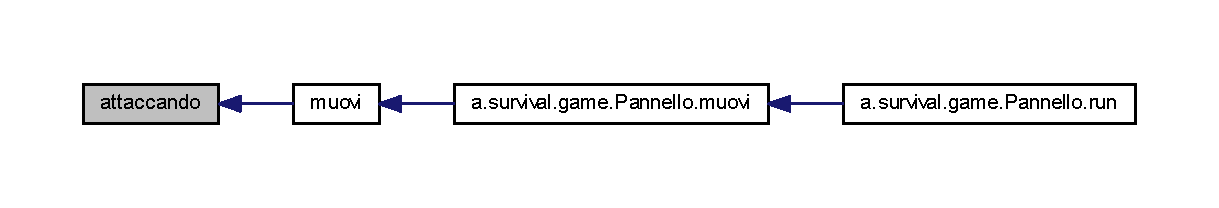
\includegraphics[width=350pt]{class_entita_1_1_giocatore_af4bcd86c7ccc1775a5fece50849563fe_icgraph}
\end{center}
\end{figure}
\mbox{\Hypertarget{class_entita_1_1_giocatore_a867fc5532a9f20042ecde7951b83c499}\label{class_entita_1_1_giocatore_a867fc5532a9f20042ecde7951b83c499}} 
\index{Entita\+::\+Giocatore@{Entita\+::\+Giocatore}!contatto\+Nemici@{contatto\+Nemici}}
\index{contatto\+Nemici@{contatto\+Nemici}!Entita\+::\+Giocatore@{Entita\+::\+Giocatore}}
\subsubsection{\texorpdfstring{contatto\+Nemici()}{contattoNemici()}}
{\footnotesize\ttfamily void contatto\+Nemici (\begin{DoxyParamCaption}\item[{int}]{i }\end{DoxyParamCaption})}



Definition at line 297 of file Giocatore.\+java.

Here is the caller graph for this function\+:
\nopagebreak
\begin{figure}[H]
\begin{center}
\leavevmode
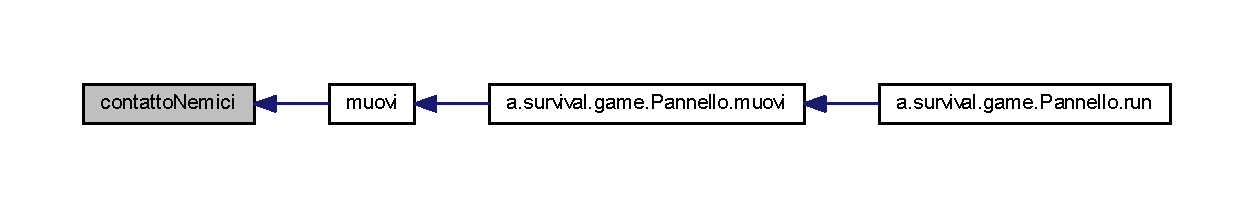
\includegraphics[width=350pt]{class_entita_1_1_giocatore_a867fc5532a9f20042ecde7951b83c499_icgraph}
\end{center}
\end{figure}
\mbox{\Hypertarget{class_entita_1_1_giocatore_a0814609fcd5c78e217a57e65bb65f7b4}\label{class_entita_1_1_giocatore_a0814609fcd5c78e217a57e65bb65f7b4}} 
\index{Entita\+::\+Giocatore@{Entita\+::\+Giocatore}!danno\+Nemico@{danno\+Nemico}}
\index{danno\+Nemico@{danno\+Nemico}!Entita\+::\+Giocatore@{Entita\+::\+Giocatore}}
\subsubsection{\texorpdfstring{danno\+Nemico()}{dannoNemico()}}
{\footnotesize\ttfamily void danno\+Nemico (\begin{DoxyParamCaption}\item[{int}]{i }\end{DoxyParamCaption})}



quando attacco i nemici diventano involnerabili per breve tempo 


\begin{DoxyParams}{Parameters}
{\em i} & \\
\hline
\end{DoxyParams}


Definition at line 312 of file Giocatore.\+java.

Here is the caller graph for this function\+:
\nopagebreak
\begin{figure}[H]
\begin{center}
\leavevmode
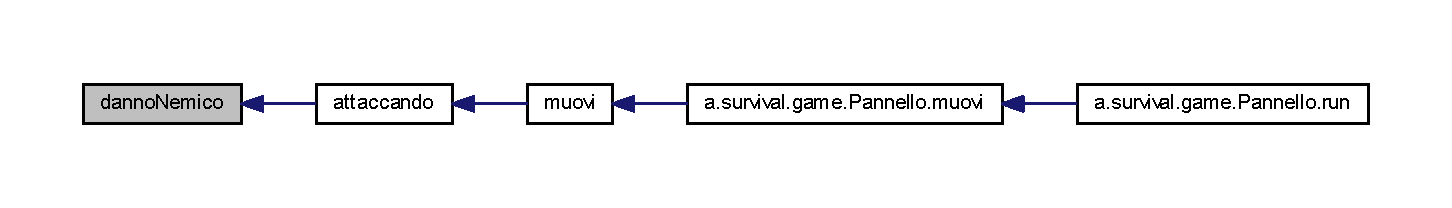
\includegraphics[width=350pt]{class_entita_1_1_giocatore_a0814609fcd5c78e217a57e65bb65f7b4_icgraph}
\end{center}
\end{figure}
\mbox{\Hypertarget{class_entita_1_1_giocatore_ae8c972c0fb4fcbc09c2219dd32cbd053}\label{class_entita_1_1_giocatore_ae8c972c0fb4fcbc09c2219dd32cbd053}} 
\index{Entita\+::\+Giocatore@{Entita\+::\+Giocatore}!draw@{draw}}
\index{draw@{draw}!Entita\+::\+Giocatore@{Entita\+::\+Giocatore}}
\subsubsection{\texorpdfstring{draw()}{draw()}}
{\footnotesize\ttfamily void draw (\begin{DoxyParamCaption}\item[{Graphics2D}]{g2 }\end{DoxyParamCaption})}



Metodo draw per printare sullo schermo tali immagini. 


\begin{DoxyParams}{Parameters}
{\em g2} & \\
\hline
\end{DoxyParams}


Definition at line 330 of file Giocatore.\+java.

\mbox{\Hypertarget{class_entita_1_1_giocatore_aafeab2e7e3b0e536c594b5aef8c31683}\label{class_entita_1_1_giocatore_aafeab2e7e3b0e536c594b5aef8c31683}} 
\index{Entita\+::\+Giocatore@{Entita\+::\+Giocatore}!get\+Attacco@{get\+Attacco}}
\index{get\+Attacco@{get\+Attacco}!Entita\+::\+Giocatore@{Entita\+::\+Giocatore}}
\subsubsection{\texorpdfstring{get\+Attacco()}{getAttacco()}}
{\footnotesize\ttfamily int get\+Attacco (\begin{DoxyParamCaption}{ }\end{DoxyParamCaption})}



Definition at line 112 of file Giocatore.\+java.

Here is the caller graph for this function\+:
\nopagebreak
\begin{figure}[H]
\begin{center}
\leavevmode
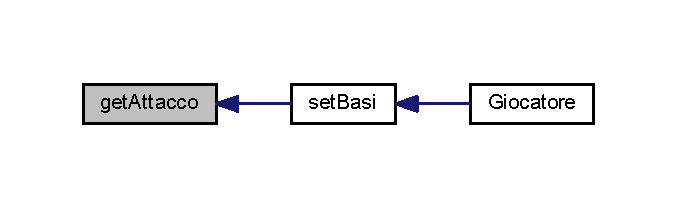
\includegraphics[width=325pt]{class_entita_1_1_giocatore_aafeab2e7e3b0e536c594b5aef8c31683_icgraph}
\end{center}
\end{figure}
\mbox{\Hypertarget{class_entita_1_1_giocatore_a5cd7986fb28ad7739710f90e464b1b27}\label{class_entita_1_1_giocatore_a5cd7986fb28ad7739710f90e464b1b27}} 
\index{Entita\+::\+Giocatore@{Entita\+::\+Giocatore}!get\+Difesa@{get\+Difesa}}
\index{get\+Difesa@{get\+Difesa}!Entita\+::\+Giocatore@{Entita\+::\+Giocatore}}
\subsubsection{\texorpdfstring{get\+Difesa()}{getDifesa()}}
{\footnotesize\ttfamily int get\+Difesa (\begin{DoxyParamCaption}{ }\end{DoxyParamCaption})}



Definition at line 116 of file Giocatore.\+java.

Here is the caller graph for this function\+:
\nopagebreak
\begin{figure}[H]
\begin{center}
\leavevmode
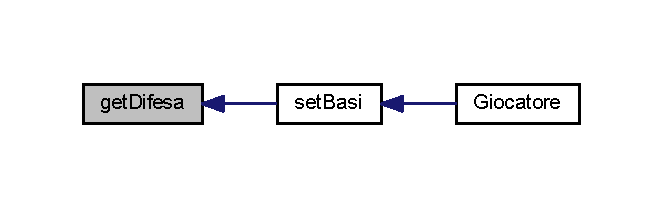
\includegraphics[width=318pt]{class_entita_1_1_giocatore_a5cd7986fb28ad7739710f90e464b1b27_icgraph}
\end{center}
\end{figure}
\mbox{\Hypertarget{class_entita_1_1_giocatore_acc1691c076ed9335796eac421dce845f}\label{class_entita_1_1_giocatore_acc1691c076ed9335796eac421dce845f}} 
\index{Entita\+::\+Giocatore@{Entita\+::\+Giocatore}!get\+Immagine\+AttaccoG@{get\+Immagine\+AttaccoG}}
\index{get\+Immagine\+AttaccoG@{get\+Immagine\+AttaccoG}!Entita\+::\+Giocatore@{Entita\+::\+Giocatore}}
\subsubsection{\texorpdfstring{get\+Immagine\+Attacco\+G()}{getImmagineAttaccoG()}}
{\footnotesize\ttfamily void get\+Immagine\+AttaccoG (\begin{DoxyParamCaption}{ }\end{DoxyParamCaption})}



setto le immagini quando attacco 



Definition at line 137 of file Giocatore.\+java.

Here is the call graph for this function\+:
\nopagebreak
\begin{figure}[H]
\begin{center}
\leavevmode
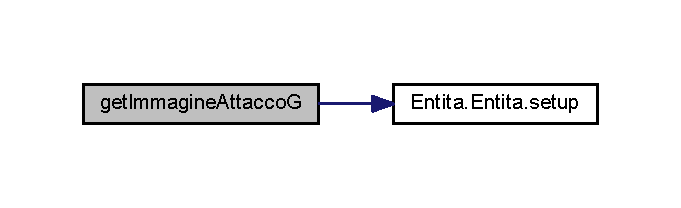
\includegraphics[width=327pt]{class_entita_1_1_giocatore_acc1691c076ed9335796eac421dce845f_cgraph}
\end{center}
\end{figure}
Here is the caller graph for this function\+:
\nopagebreak
\begin{figure}[H]
\begin{center}
\leavevmode
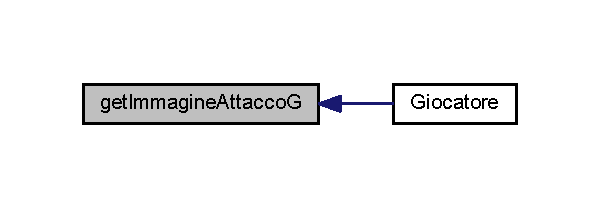
\includegraphics[width=288pt]{class_entita_1_1_giocatore_acc1691c076ed9335796eac421dce845f_icgraph}
\end{center}
\end{figure}
\mbox{\Hypertarget{class_entita_1_1_giocatore_abac365540bed82b4025e8e845b779c72}\label{class_entita_1_1_giocatore_abac365540bed82b4025e8e845b779c72}} 
\index{Entita\+::\+Giocatore@{Entita\+::\+Giocatore}!get\+ImmagineG@{get\+ImmagineG}}
\index{get\+ImmagineG@{get\+ImmagineG}!Entita\+::\+Giocatore@{Entita\+::\+Giocatore}}
\subsubsection{\texorpdfstring{get\+Immagine\+G()}{getImmagineG()}}
{\footnotesize\ttfamily void get\+ImmagineG (\begin{DoxyParamCaption}{ }\end{DoxyParamCaption})}



setto le immagini quando cammino 



Definition at line 123 of file Giocatore.\+java.

Here is the call graph for this function\+:
\nopagebreak
\begin{figure}[H]
\begin{center}
\leavevmode
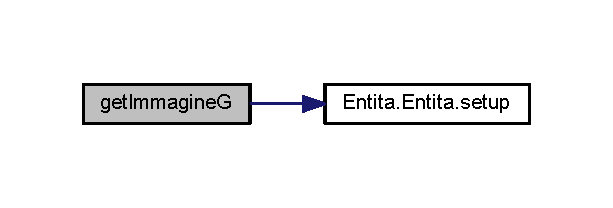
\includegraphics[width=294pt]{class_entita_1_1_giocatore_abac365540bed82b4025e8e845b779c72_cgraph}
\end{center}
\end{figure}
Here is the caller graph for this function\+:
\nopagebreak
\begin{figure}[H]
\begin{center}
\leavevmode
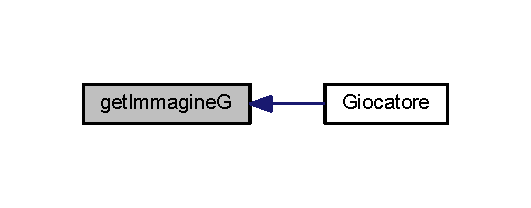
\includegraphics[width=255pt]{class_entita_1_1_giocatore_abac365540bed82b4025e8e845b779c72_icgraph}
\end{center}
\end{figure}
\mbox{\Hypertarget{class_entita_1_1_giocatore_aaf1d3a52e79be598afe385c91a9f4d0c}\label{class_entita_1_1_giocatore_aaf1d3a52e79be598afe385c91a9f4d0c}} 
\index{Entita\+::\+Giocatore@{Entita\+::\+Giocatore}!interaz\+N\+PC@{interaz\+N\+PC}}
\index{interaz\+N\+PC@{interaz\+N\+PC}!Entita\+::\+Giocatore@{Entita\+::\+Giocatore}}
\subsubsection{\texorpdfstring{interaz\+N\+P\+C()}{interazNPC()}}
{\footnotesize\ttfamily void interaz\+N\+PC (\begin{DoxyParamCaption}\item[{int}]{i }\end{DoxyParamCaption})}



Definition at line 284 of file Giocatore.\+java.

Here is the caller graph for this function\+:
\nopagebreak
\begin{figure}[H]
\begin{center}
\leavevmode
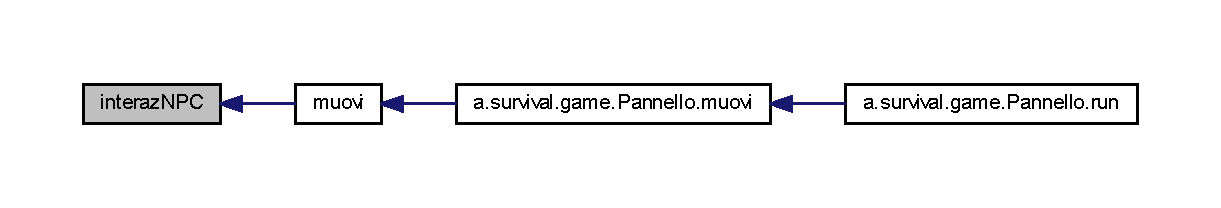
\includegraphics[width=350pt]{class_entita_1_1_giocatore_aaf1d3a52e79be598afe385c91a9f4d0c_icgraph}
\end{center}
\end{figure}
\mbox{\Hypertarget{class_entita_1_1_giocatore_a1fe2f184b3cc7345c6a0f08d183a1d0b}\label{class_entita_1_1_giocatore_a1fe2f184b3cc7345c6a0f08d183a1d0b}} 
\index{Entita\+::\+Giocatore@{Entita\+::\+Giocatore}!muovi@{muovi}}
\index{muovi@{muovi}!Entita\+::\+Giocatore@{Entita\+::\+Giocatore}}
\subsubsection{\texorpdfstring{muovi()}{muovi()}}
{\footnotesize\ttfamily void muovi (\begin{DoxyParamCaption}{ }\end{DoxyParamCaption})}



Metodo per far muovere il player e per caricare in base la direzione l\textquotesingle{}immagine giusta. 



Definition at line 151 of file Giocatore.\+java.

Here is the call graph for this function\+:
\nopagebreak
\begin{figure}[H]
\begin{center}
\leavevmode
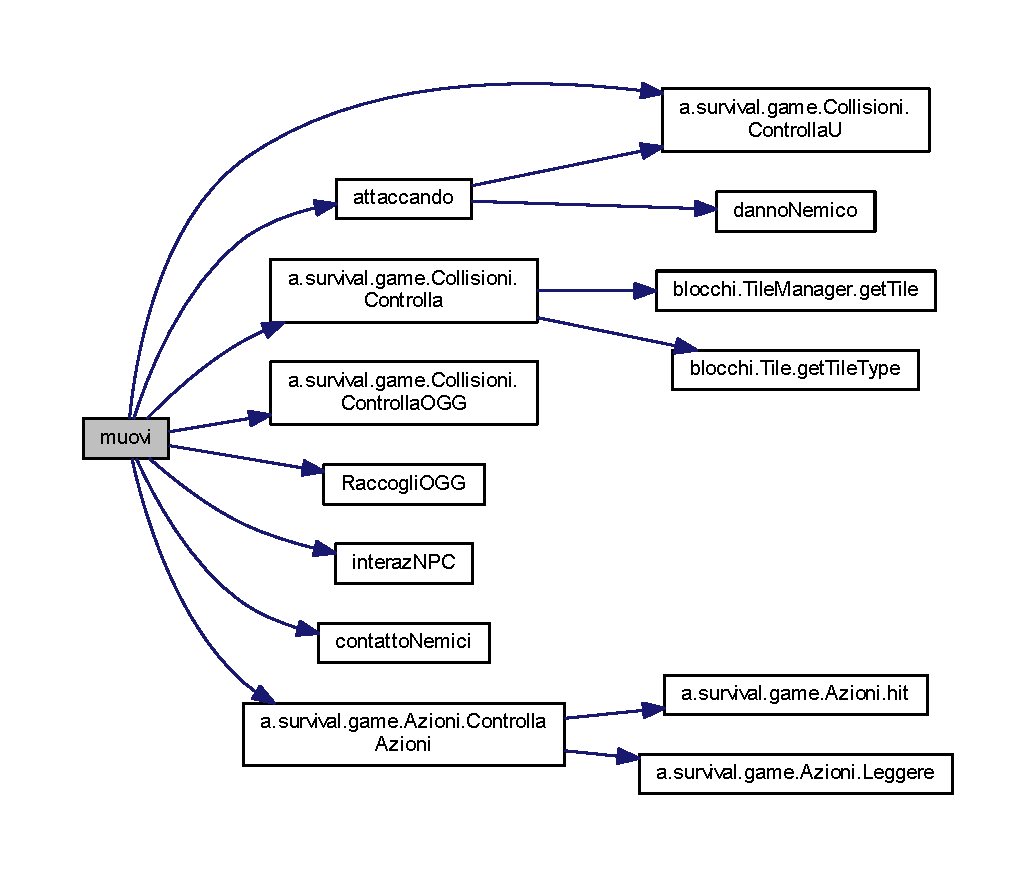
\includegraphics[width=350pt]{class_entita_1_1_giocatore_a1fe2f184b3cc7345c6a0f08d183a1d0b_cgraph}
\end{center}
\end{figure}
Here is the caller graph for this function\+:
\nopagebreak
\begin{figure}[H]
\begin{center}
\leavevmode
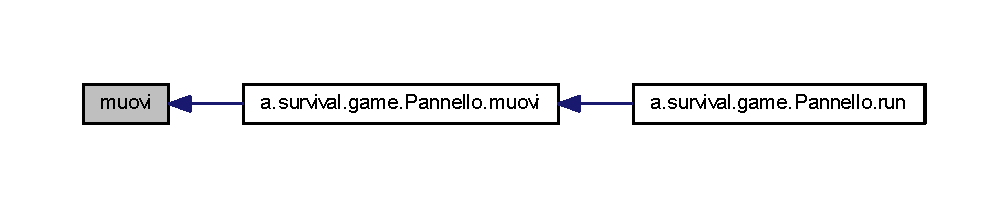
\includegraphics[width=350pt]{class_entita_1_1_giocatore_a1fe2f184b3cc7345c6a0f08d183a1d0b_icgraph}
\end{center}
\end{figure}
\mbox{\Hypertarget{class_entita_1_1_giocatore_a9ba65e7d25928d62218cf14bee3c0273}\label{class_entita_1_1_giocatore_a9ba65e7d25928d62218cf14bee3c0273}} 
\index{Entita\+::\+Giocatore@{Entita\+::\+Giocatore}!Raccogli\+O\+GG@{Raccogli\+O\+GG}}
\index{Raccogli\+O\+GG@{Raccogli\+O\+GG}!Entita\+::\+Giocatore@{Entita\+::\+Giocatore}}
\subsubsection{\texorpdfstring{Raccogli\+O\+G\+G()}{RaccogliOGG()}}
{\footnotesize\ttfamily void Raccogli\+O\+GG (\begin{DoxyParamCaption}\item[{int}]{i }\end{DoxyParamCaption})}



Definition at line 278 of file Giocatore.\+java.

Here is the caller graph for this function\+:
\nopagebreak
\begin{figure}[H]
\begin{center}
\leavevmode
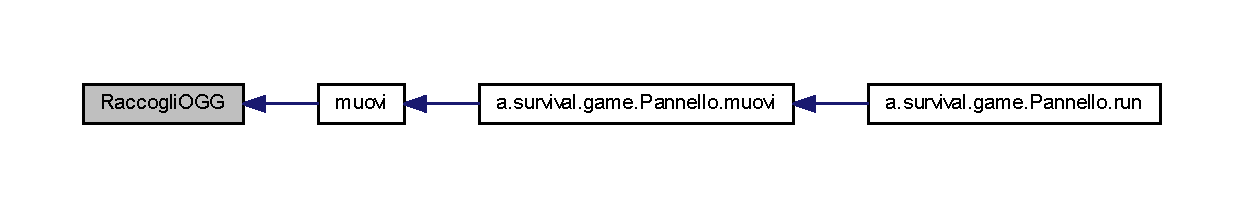
\includegraphics[width=350pt]{class_entita_1_1_giocatore_a9ba65e7d25928d62218cf14bee3c0273_icgraph}
\end{center}
\end{figure}
\mbox{\Hypertarget{class_entita_1_1_giocatore_a38a75be5807f155ff640bfa73518421d}\label{class_entita_1_1_giocatore_a38a75be5807f155ff640bfa73518421d}} 
\index{Entita\+::\+Giocatore@{Entita\+::\+Giocatore}!set\+Basi@{set\+Basi}}
\index{set\+Basi@{set\+Basi}!Entita\+::\+Giocatore@{Entita\+::\+Giocatore}}
\subsubsection{\texorpdfstring{set\+Basi()}{setBasi()}}
{\footnotesize\ttfamily void set\+Basi (\begin{DoxyParamCaption}{ }\end{DoxyParamCaption})}



Metodo per settare i valori base del giocatore. 

x dove spawna

y dove spawna

velocita

direzione fissa quando spawna

vita

più forza hai, più colpisci forte

più spirito hai, più sei invulnerabile

Definition at line 81 of file Giocatore.\+java.

Here is the call graph for this function\+:
\nopagebreak
\begin{figure}[H]
\begin{center}
\leavevmode
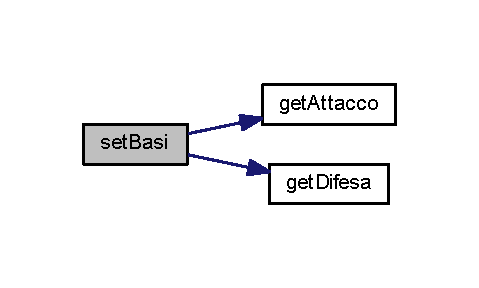
\includegraphics[width=230pt]{class_entita_1_1_giocatore_a38a75be5807f155ff640bfa73518421d_cgraph}
\end{center}
\end{figure}
Here is the caller graph for this function\+:
\nopagebreak
\begin{figure}[H]
\begin{center}
\leavevmode
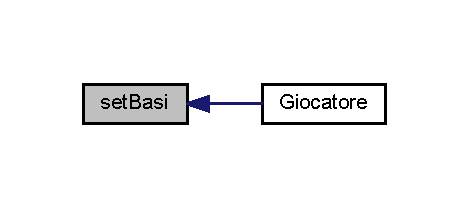
\includegraphics[width=225pt]{class_entita_1_1_giocatore_a38a75be5807f155ff640bfa73518421d_icgraph}
\end{center}
\end{figure}


\subsection{Member Data Documentation}
\mbox{\Hypertarget{class_entita_1_1_giocatore_ade56944373ebbc5f5117b39639e3cef5}\label{class_entita_1_1_giocatore_ade56944373ebbc5f5117b39639e3cef5}} 
\index{Entita\+::\+Giocatore@{Entita\+::\+Giocatore}!Arma@{Arma}}
\index{Arma@{Arma}!Entita\+::\+Giocatore@{Entita\+::\+Giocatore}}
\subsubsection{\texorpdfstring{Arma}{Arma}}
{\footnotesize\ttfamily \hyperlink{class_entita_1_1_entita}{Entita} Arma}



Definition at line 35 of file Giocatore.\+java.

\mbox{\Hypertarget{class_entita_1_1_giocatore_a585c716c79ac39d627dd9719b902a64f}\label{class_entita_1_1_giocatore_a585c716c79ac39d627dd9719b902a64f}} 
\index{Entita\+::\+Giocatore@{Entita\+::\+Giocatore}!attacco@{attacco}}
\index{attacco@{attacco}!Entita\+::\+Giocatore@{Entita\+::\+Giocatore}}
\subsubsection{\texorpdfstring{attacco}{attacco}}
{\footnotesize\ttfamily int attacco}



Definition at line 30 of file Giocatore.\+java.

\mbox{\Hypertarget{class_entita_1_1_giocatore_a955d461d95cf97cd1806f6abc44ce485}\label{class_entita_1_1_giocatore_a955d461d95cf97cd1806f6abc44ce485}} 
\index{Entita\+::\+Giocatore@{Entita\+::\+Giocatore}!attacco\+Spada@{attacco\+Spada}}
\index{attacco\+Spada@{attacco\+Spada}!Entita\+::\+Giocatore@{Entita\+::\+Giocatore}}
\subsubsection{\texorpdfstring{attacco\+Spada}{attaccoSpada}}
{\footnotesize\ttfamily int attacco\+Spada}

statistiche armi 

Definition at line 39 of file Giocatore.\+java.

\mbox{\Hypertarget{class_entita_1_1_giocatore_a738b89ee909e3e3b2751a2fa9a959813}\label{class_entita_1_1_giocatore_a738b89ee909e3e3b2751a2fa9a959813}} 
\index{Entita\+::\+Giocatore@{Entita\+::\+Giocatore}!attacco\+Su1@{attacco\+Su1}}
\index{attacco\+Su1@{attacco\+Su1}!Entita\+::\+Giocatore@{Entita\+::\+Giocatore}}
\subsubsection{\texorpdfstring{attacco\+Su1}{attaccoSu1}}
{\footnotesize\ttfamily Buffered\+Image attacco\+Su1}

setto immagi per quando attacca ill giocatore 

Definition at line 25 of file Giocatore.\+java.

\mbox{\Hypertarget{class_entita_1_1_giocatore_a0ace2881b0b5e4e097b5f406cb9d173b}\label{class_entita_1_1_giocatore_a0ace2881b0b5e4e097b5f406cb9d173b}} 
\index{Entita\+::\+Giocatore@{Entita\+::\+Giocatore}!Cont\+Attacchi@{Cont\+Attacchi}}
\index{Cont\+Attacchi@{Cont\+Attacchi}!Entita\+::\+Giocatore@{Entita\+::\+Giocatore}}
\subsubsection{\texorpdfstring{Cont\+Attacchi}{ContAttacchi}}
{\footnotesize\ttfamily boolean Cont\+Attacchi = false}



Definition at line 49 of file Giocatore.\+java.

\mbox{\Hypertarget{class_entita_1_1_giocatore_afdf43c12f58b193223e199b997834e59}\label{class_entita_1_1_giocatore_afdf43c12f58b193223e199b997834e59}} 
\index{Entita\+::\+Giocatore@{Entita\+::\+Giocatore}!difesa@{difesa}}
\index{difesa@{difesa}!Entita\+::\+Giocatore@{Entita\+::\+Giocatore}}
\subsubsection{\texorpdfstring{difesa}{difesa}}
{\footnotesize\ttfamily int difesa}



Definition at line 31 of file Giocatore.\+java.

\mbox{\Hypertarget{class_entita_1_1_giocatore_ad1c7c7fe90e4e2563cac9ed38ccb479d}\label{class_entita_1_1_giocatore_ad1c7c7fe90e4e2563cac9ed38ccb479d}} 
\index{Entita\+::\+Giocatore@{Entita\+::\+Giocatore}!difesa\+Scudo@{difesa\+Scudo}}
\index{difesa\+Scudo@{difesa\+Scudo}!Entita\+::\+Giocatore@{Entita\+::\+Giocatore}}
\subsubsection{\texorpdfstring{difesa\+Scudo}{difesaScudo}}
{\footnotesize\ttfamily int difesa\+Scudo}



Definition at line 40 of file Giocatore.\+java.

\mbox{\Hypertarget{class_entita_1_1_giocatore_a3bb4af16b31e7979f424cf66f1bfa6e2}\label{class_entita_1_1_giocatore_a3bb4af16b31e7979f424cf66f1bfa6e2}} 
\index{Entita\+::\+Giocatore@{Entita\+::\+Giocatore}!exp@{exp}}
\index{exp@{exp}!Entita\+::\+Giocatore@{Entita\+::\+Giocatore}}
\subsubsection{\texorpdfstring{exp}{exp}}
{\footnotesize\ttfamily int exp}



Definition at line 33 of file Giocatore.\+java.

\mbox{\Hypertarget{class_entita_1_1_giocatore_a11a8dccab7cd0e8facbe3152140e41b8}\label{class_entita_1_1_giocatore_a11a8dccab7cd0e8facbe3152140e41b8}} 
\index{Entita\+::\+Giocatore@{Entita\+::\+Giocatore}!forza@{forza}}
\index{forza@{forza}!Entita\+::\+Giocatore@{Entita\+::\+Giocatore}}
\subsubsection{\texorpdfstring{forza}{forza}}
{\footnotesize\ttfamily int forza}



Definition at line 29 of file Giocatore.\+java.

\mbox{\Hypertarget{class_entita_1_1_giocatore_a9df9739330535dcec4121b7a25289af6}\label{class_entita_1_1_giocatore_a9df9739330535dcec4121b7a25289af6}} 
\index{Entita\+::\+Giocatore@{Entita\+::\+Giocatore}!livello@{livello}}
\index{livello@{livello}!Entita\+::\+Giocatore@{Entita\+::\+Giocatore}}
\subsubsection{\texorpdfstring{livello}{livello}}
{\footnotesize\ttfamily int livello}

statistiche giocatore 

Definition at line 28 of file Giocatore.\+java.

\mbox{\Hypertarget{class_entita_1_1_giocatore_a446b75d761c1ca3d631eaa61b04298d2}\label{class_entita_1_1_giocatore_a446b75d761c1ca3d631eaa61b04298d2}} 
\index{Entita\+::\+Giocatore@{Entita\+::\+Giocatore}!schermoX@{schermoX}}
\index{schermoX@{schermoX}!Entita\+::\+Giocatore@{Entita\+::\+Giocatore}}
\subsubsection{\texorpdfstring{schermoX}{schermoX}}
{\footnotesize\ttfamily final int schermoX}



Definition at line 44 of file Giocatore.\+java.

\mbox{\Hypertarget{class_entita_1_1_giocatore_ada8f80a3f9f6b62953b85f6d05d02c50}\label{class_entita_1_1_giocatore_ada8f80a3f9f6b62953b85f6d05d02c50}} 
\index{Entita\+::\+Giocatore@{Entita\+::\+Giocatore}!schermoY@{schermoY}}
\index{schermoY@{schermoY}!Entita\+::\+Giocatore@{Entita\+::\+Giocatore}}
\subsubsection{\texorpdfstring{schermoY}{schermoY}}
{\footnotesize\ttfamily final int schermoY}



Definition at line 45 of file Giocatore.\+java.

\mbox{\Hypertarget{class_entita_1_1_giocatore_a07e5f7f5db8ac85356757f54f153bb20}\label{class_entita_1_1_giocatore_a07e5f7f5db8ac85356757f54f153bb20}} 
\index{Entita\+::\+Giocatore@{Entita\+::\+Giocatore}!Scudo@{Scudo}}
\index{Scudo@{Scudo}!Entita\+::\+Giocatore@{Entita\+::\+Giocatore}}
\subsubsection{\texorpdfstring{Scudo}{Scudo}}
{\footnotesize\ttfamily \hyperlink{class_entita_1_1_entita}{Entita} Scudo}



Definition at line 36 of file Giocatore.\+java.

\mbox{\Hypertarget{class_entita_1_1_giocatore_a4ab2b490b2927b4d21ee663f63f81bd6}\label{class_entita_1_1_giocatore_a4ab2b490b2927b4d21ee663f63f81bd6}} 
\index{Entita\+::\+Giocatore@{Entita\+::\+Giocatore}!soldi@{soldi}}
\index{soldi@{soldi}!Entita\+::\+Giocatore@{Entita\+::\+Giocatore}}
\subsubsection{\texorpdfstring{soldi}{soldi}}
{\footnotesize\ttfamily int soldi}



Definition at line 34 of file Giocatore.\+java.

\mbox{\Hypertarget{class_entita_1_1_giocatore_a531fc785df2ee9bd58da74a801e766c4}\label{class_entita_1_1_giocatore_a531fc785df2ee9bd58da74a801e766c4}} 
\index{Entita\+::\+Giocatore@{Entita\+::\+Giocatore}!spirito@{spirito}}
\index{spirito@{spirito}!Entita\+::\+Giocatore@{Entita\+::\+Giocatore}}
\subsubsection{\texorpdfstring{spirito}{spirito}}
{\footnotesize\ttfamily int spirito}



Definition at line 32 of file Giocatore.\+java.



The documentation for this class was generated from the following file\+:\begin{DoxyCompactItemize}
\item 
src/\+Entita/\hyperlink{_giocatore_8java}{Giocatore.\+java}\end{DoxyCompactItemize}

\hypertarget{classa_1_1survival_1_1game_1_1_interfaccia}{}\section{Interfaccia Class Reference}
\label{classa_1_1survival_1_1game_1_1_interfaccia}\index{Interfaccia@{Interfaccia}}


Collaboration diagram for Interfaccia\+:
\nopagebreak
\begin{figure}[H]
\begin{center}
\leavevmode
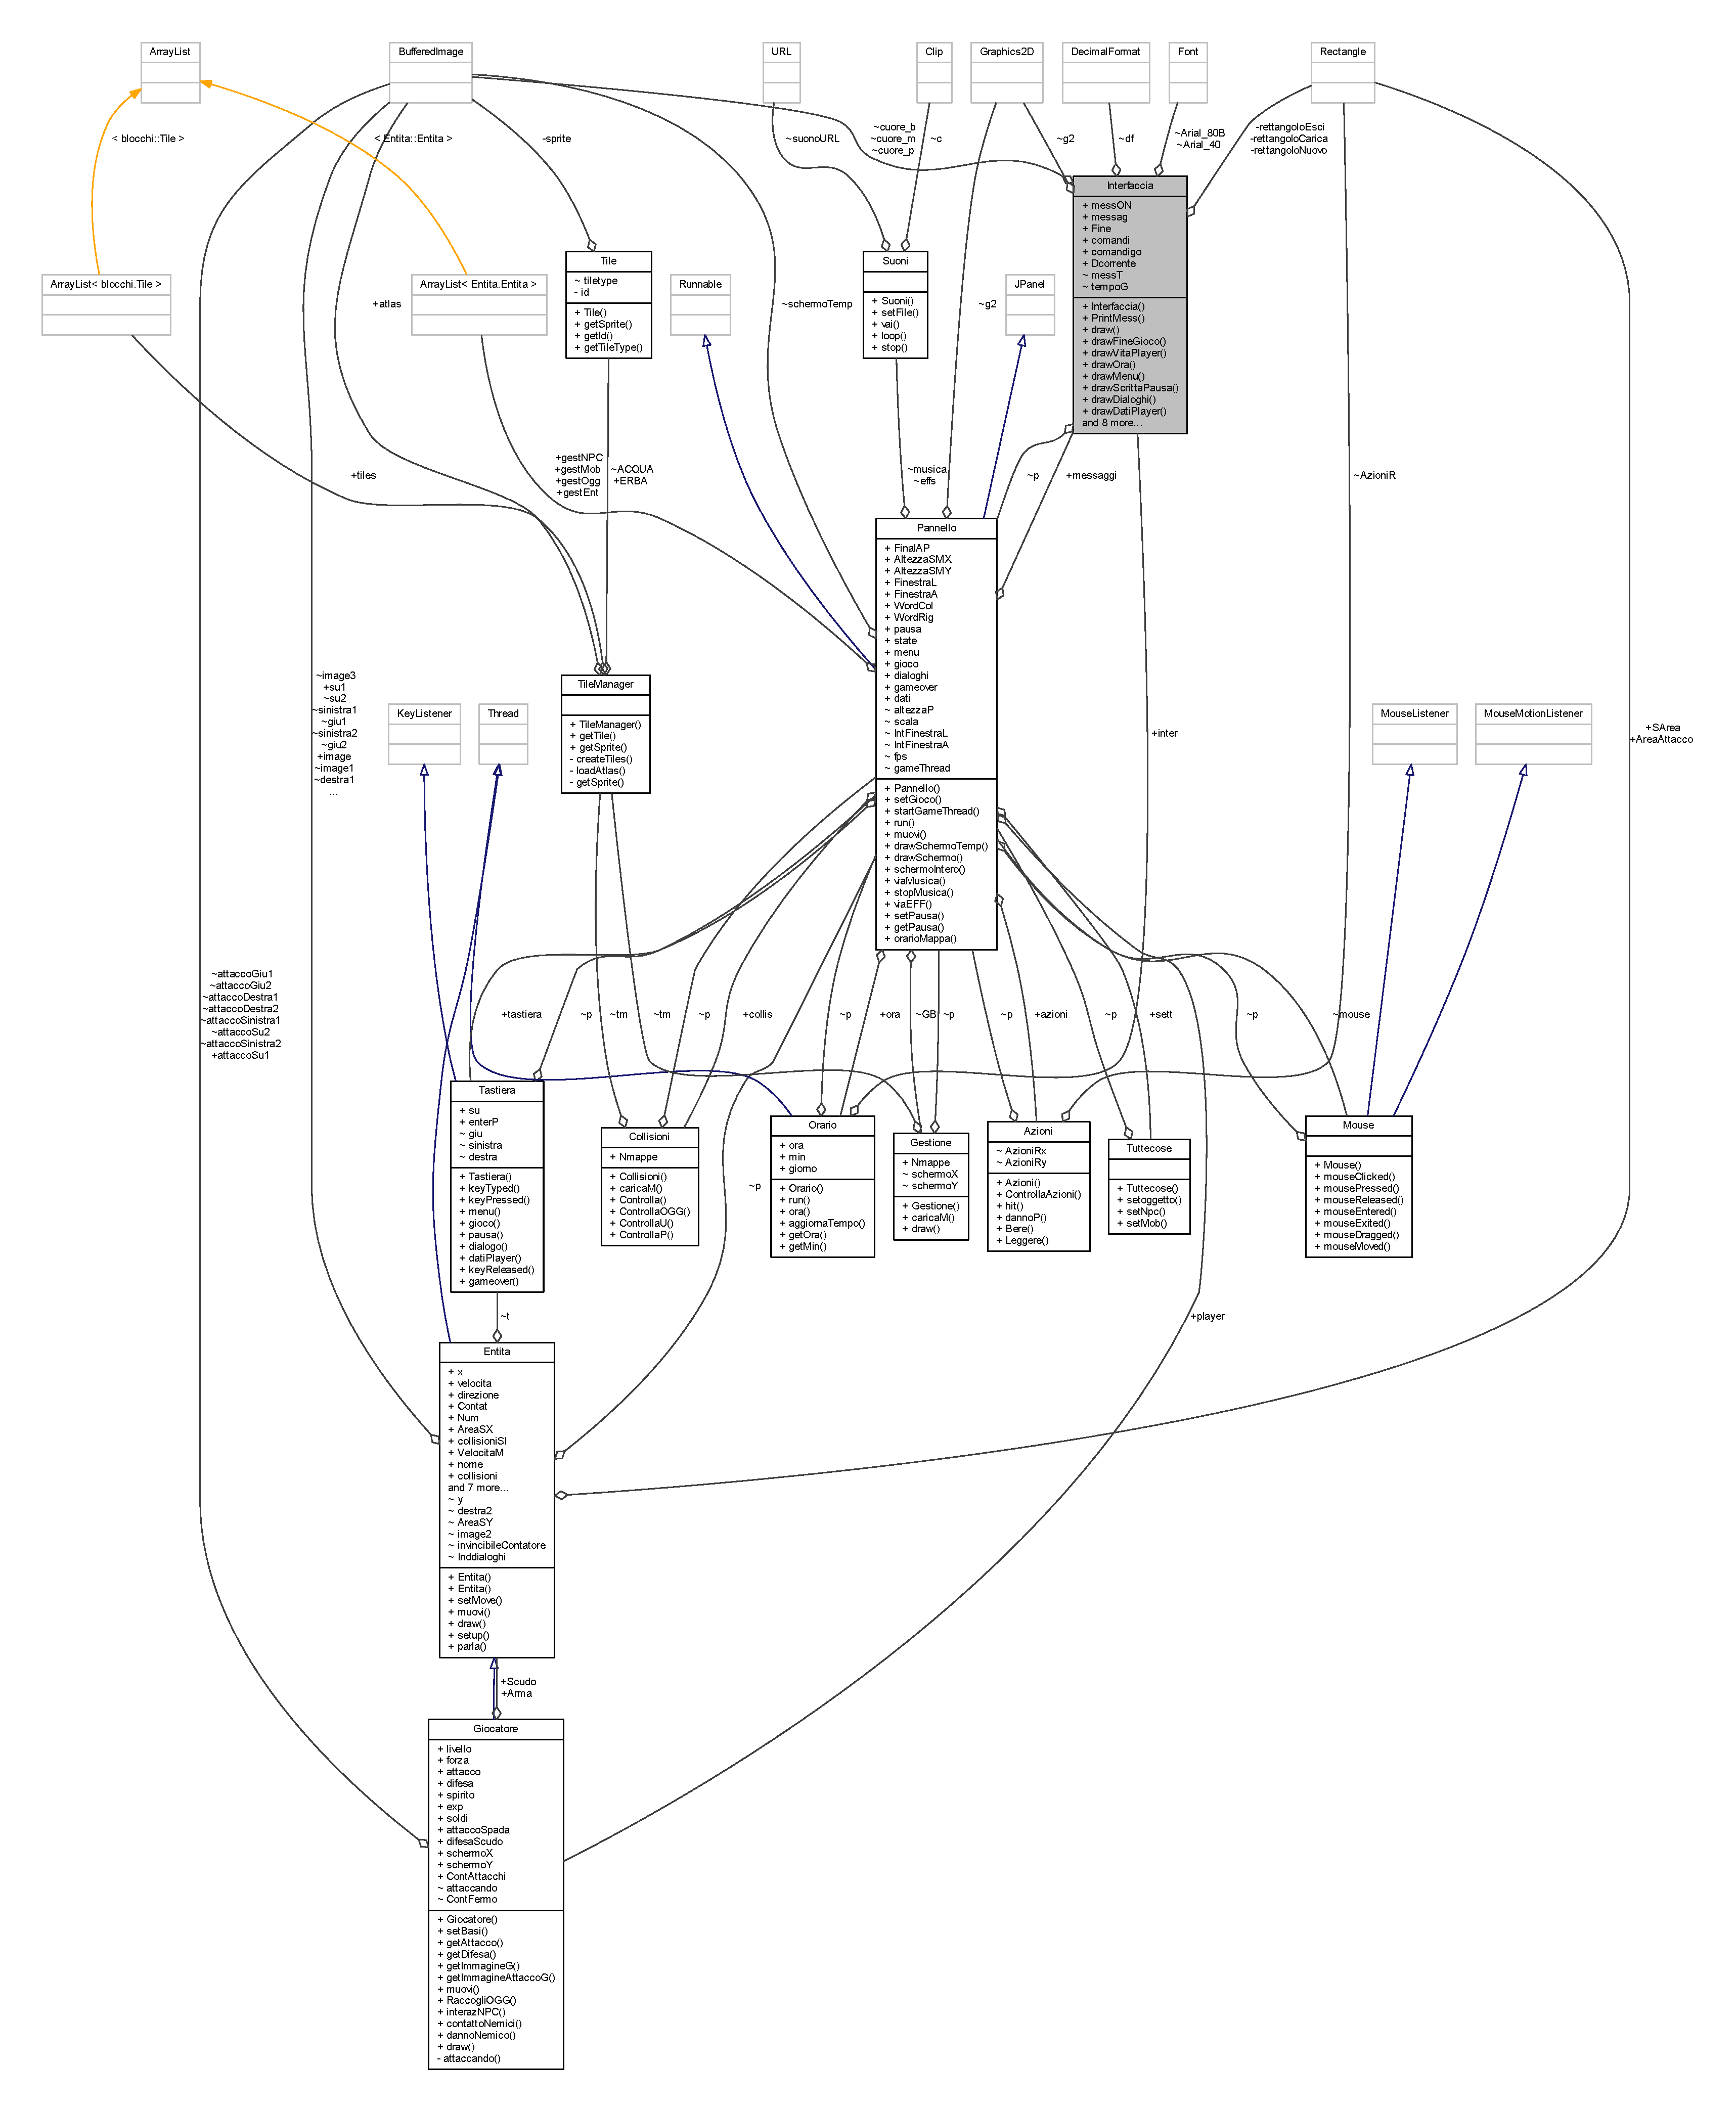
\includegraphics[width=350pt]{classa_1_1survival_1_1game_1_1_interfaccia__coll__graph}
\end{center}
\end{figure}
\subsection*{Public Member Functions}
\begin{DoxyCompactItemize}
\item 
\hyperlink{classa_1_1survival_1_1game_1_1_interfaccia_adcff06a15c5f6ba258455f184dd915fb}{Interfaccia} (\hyperlink{classa_1_1survival_1_1game_1_1_pannello}{Pannello} p)
\item 
void \hyperlink{classa_1_1survival_1_1game_1_1_interfaccia_ae9b898a41ae435279045781f39227899}{Print\+Mess} (String testo)
\item 
void \hyperlink{classa_1_1survival_1_1game_1_1_interfaccia_ae8c972c0fb4fcbc09c2219dd32cbd053}{draw} (Graphics2D g2)
\begin{DoxyCompactList}\small\item\em Metodo draw per printare i messaggi. \end{DoxyCompactList}\item 
void \hyperlink{classa_1_1survival_1_1game_1_1_interfaccia_afb3918edf3e2da123a3585258d5c5045}{draw\+Fine\+Gioco} ()
\begin{DoxyCompactList}\small\item\em Metodo per printare la scritta di fine gioco. \end{DoxyCompactList}\item 
void \hyperlink{classa_1_1survival_1_1game_1_1_interfaccia_a24697f9d9cd1d55fc26a7b7c0fd26697}{draw\+Vita\+Player} ()
\begin{DoxyCompactList}\small\item\em Metodo per printare la vita del giocatore. \end{DoxyCompactList}\item 
void \hyperlink{classa_1_1survival_1_1game_1_1_interfaccia_a2dc05af87e20aefac5da3cd184d09456}{draw\+Ora} (String ora)
\begin{DoxyCompactList}\small\item\em Metodo per printare l\textquotesingle{}ora nel gioco. \end{DoxyCompactList}\item 
void \hyperlink{classa_1_1survival_1_1game_1_1_interfaccia_aa13653318c21b0e6b86838e6091bfc9a}{draw\+Menu} ()
\begin{DoxyCompactList}\small\item\em Metodo per printare il menu. \end{DoxyCompactList}\item 
void \hyperlink{classa_1_1survival_1_1game_1_1_interfaccia_a5ea2e0aa29eed2ee8e977ec1495103d3}{draw\+Scritta\+Pausa} ()
\begin{DoxyCompactList}\small\item\em Metodo per printare la scritta pausa. \end{DoxyCompactList}\item 
void \hyperlink{classa_1_1survival_1_1game_1_1_interfaccia_a07761ecd195353aa0f33107b57c3c852}{draw\+Dialoghi} ()
\begin{DoxyCompactList}\small\item\em Metodo per printare i dialoghi tra npc e player. \end{DoxyCompactList}\item 
void \hyperlink{classa_1_1survival_1_1game_1_1_interfaccia_aa9a8046a21bf4083e12263a078701107}{draw\+Dati\+Player} ()
\begin{DoxyCompactList}\small\item\em Metodo per printare le statisctiche del giocatore. \end{DoxyCompactList}\item 
void \hyperlink{classa_1_1survival_1_1game_1_1_interfaccia_a73a0c3b24b1d27132d84f43de7262e36}{draw\+DialoghiF} (int x, int y, int larghezza, int altezza)
\item 
int \hyperlink{classa_1_1survival_1_1game_1_1_interfaccia_a33bfff0e4091d0c94334a82514ffa7ec}{get\+X\+Testo\+Centrato} (String testo)
\item 
int \hyperlink{classa_1_1survival_1_1game_1_1_interfaccia_a587ecc556d77a50194f3e80ca09551ce}{get\+X\+Testo\+Adestra} (String testo, int parolaX)
\item 
int \hyperlink{classa_1_1survival_1_1game_1_1_interfaccia_a5e33eb51424c4888d0cd26cf5e0311de}{get\+Lunghezza\+Stringa} (String testo)
\item 
int \hyperlink{classa_1_1survival_1_1game_1_1_interfaccia_af3e544b837451de1ad271a8d32b61385}{get\+Altezza\+Stringa} (String testo)
\item 
void \hyperlink{classa_1_1survival_1_1game_1_1_interfaccia_a2ca251710b65639ec80bc141edde60aa}{mouse\+Moved} (Mouse\+Event e)
\item 
void \hyperlink{classa_1_1survival_1_1game_1_1_interfaccia_a45d56bd84238e8b56589dfc732e2b2cf}{mouse\+Clicked} (Mouse\+Event e)
\item 
void \hyperlink{classa_1_1survival_1_1game_1_1_interfaccia_aeb2c7e9c7d14c9eccb7e624bd9611ef8}{draw\+Game\+Over} ()
\end{DoxyCompactItemize}
\subsection*{Public Attributes}
\begin{DoxyCompactItemize}
\item 
boolean \hyperlink{classa_1_1survival_1_1game_1_1_interfaccia_a53638d8b01e1903b2c724ef960d9d51d}{mess\+ON} = false
\item 
String \hyperlink{classa_1_1survival_1_1game_1_1_interfaccia_abe702b74b2a1a486bd641ce9b6c56f79}{messag} = \char`\"{}\char`\"{}
\item 
boolean \hyperlink{classa_1_1survival_1_1game_1_1_interfaccia_af01195fe9c733fd0a6c3eebcf8b31777}{Fine} =false
\item 
int \hyperlink{classa_1_1survival_1_1game_1_1_interfaccia_a649a8655713bf0e8464a2a3a957c26d4}{comandi} = 0
\item 
int \hyperlink{classa_1_1survival_1_1game_1_1_interfaccia_aa1be8778fa46376bbd32e59db2ed3a33}{comandigo} = 0
\item 
String \hyperlink{classa_1_1survival_1_1game_1_1_interfaccia_a642bb62c6c1f15bd181a60884ced61b7}{Dcorrente} = \char`\"{}\char`\"{}
\end{DoxyCompactItemize}
\subsection*{Private Attributes}
\begin{DoxyCompactItemize}
\item 
Rectangle \hyperlink{classa_1_1survival_1_1game_1_1_interfaccia_abe31ab860ef846d30a5e7b91253e3ff5}{rettangolo\+Nuovo}
\item 
Rectangle \hyperlink{classa_1_1survival_1_1game_1_1_interfaccia_a2adab04fb2a98335bebb9fa899cb60ad}{rettangolo\+Carica}
\item 
Rectangle \hyperlink{classa_1_1survival_1_1game_1_1_interfaccia_a799e22b4be0cc2c5bf997bfaf99be31b}{rettangolo\+Esci}
\end{DoxyCompactItemize}


\subsection{Detailed Description}


Definition at line 25 of file Interfaccia.\+java.



\subsection{Constructor \& Destructor Documentation}
\mbox{\Hypertarget{classa_1_1survival_1_1game_1_1_interfaccia_adcff06a15c5f6ba258455f184dd915fb}\label{classa_1_1survival_1_1game_1_1_interfaccia_adcff06a15c5f6ba258455f184dd915fb}} 
\index{a\+::survival\+::game\+::\+Interfaccia@{a\+::survival\+::game\+::\+Interfaccia}!Interfaccia@{Interfaccia}}
\index{Interfaccia@{Interfaccia}!a\+::survival\+::game\+::\+Interfaccia@{a\+::survival\+::game\+::\+Interfaccia}}
\subsubsection{\texorpdfstring{Interfaccia()}{Interfaccia()}}
{\footnotesize\ttfamily \hyperlink{classa_1_1survival_1_1game_1_1_interfaccia}{Interfaccia} (\begin{DoxyParamCaption}\item[{\hyperlink{classa_1_1survival_1_1game_1_1_pannello}{Pannello}}]{p }\end{DoxyParamCaption})}



Definition at line 44 of file Interfaccia.\+java.



\subsection{Member Function Documentation}
\mbox{\Hypertarget{classa_1_1survival_1_1game_1_1_interfaccia_ae8c972c0fb4fcbc09c2219dd32cbd053}\label{classa_1_1survival_1_1game_1_1_interfaccia_ae8c972c0fb4fcbc09c2219dd32cbd053}} 
\index{a\+::survival\+::game\+::\+Interfaccia@{a\+::survival\+::game\+::\+Interfaccia}!draw@{draw}}
\index{draw@{draw}!a\+::survival\+::game\+::\+Interfaccia@{a\+::survival\+::game\+::\+Interfaccia}}
\subsubsection{\texorpdfstring{draw()}{draw()}}
{\footnotesize\ttfamily void draw (\begin{DoxyParamCaption}\item[{Graphics2D}]{g2 }\end{DoxyParamCaption})}



Metodo draw per printare i messaggi. 


\begin{DoxyParams}{Parameters}
{\em g2} & \\
\hline
\end{DoxyParams}


Definition at line 65 of file Interfaccia.\+java.

Here is the call graph for this function\+:
\nopagebreak
\begin{figure}[H]
\begin{center}
\leavevmode
\includegraphics[width=350pt]{classa_1_1survival_1_1game_1_1_interfaccia_ae8c972c0fb4fcbc09c2219dd32cbd053_cgraph}
\end{center}
\end{figure}
Here is the caller graph for this function\+:
\nopagebreak
\begin{figure}[H]
\begin{center}
\leavevmode
\includegraphics[width=350pt]{classa_1_1survival_1_1game_1_1_interfaccia_ae8c972c0fb4fcbc09c2219dd32cbd053_icgraph}
\end{center}
\end{figure}
\mbox{\Hypertarget{classa_1_1survival_1_1game_1_1_interfaccia_aa9a8046a21bf4083e12263a078701107}\label{classa_1_1survival_1_1game_1_1_interfaccia_aa9a8046a21bf4083e12263a078701107}} 
\index{a\+::survival\+::game\+::\+Interfaccia@{a\+::survival\+::game\+::\+Interfaccia}!draw\+Dati\+Player@{draw\+Dati\+Player}}
\index{draw\+Dati\+Player@{draw\+Dati\+Player}!a\+::survival\+::game\+::\+Interfaccia@{a\+::survival\+::game\+::\+Interfaccia}}
\subsubsection{\texorpdfstring{draw\+Dati\+Player()}{drawDatiPlayer()}}
{\footnotesize\ttfamily void draw\+Dati\+Player (\begin{DoxyParamCaption}{ }\end{DoxyParamCaption})}



Metodo per printare le statisctiche del giocatore. 



Definition at line 258 of file Interfaccia.\+java.

Here is the call graph for this function\+:
\nopagebreak
\begin{figure}[H]
\begin{center}
\leavevmode
\includegraphics[width=291pt]{classa_1_1survival_1_1game_1_1_interfaccia_aa9a8046a21bf4083e12263a078701107_cgraph}
\end{center}
\end{figure}
Here is the caller graph for this function\+:
\nopagebreak
\begin{figure}[H]
\begin{center}
\leavevmode
\includegraphics[width=350pt]{classa_1_1survival_1_1game_1_1_interfaccia_aa9a8046a21bf4083e12263a078701107_icgraph}
\end{center}
\end{figure}
\mbox{\Hypertarget{classa_1_1survival_1_1game_1_1_interfaccia_a07761ecd195353aa0f33107b57c3c852}\label{classa_1_1survival_1_1game_1_1_interfaccia_a07761ecd195353aa0f33107b57c3c852}} 
\index{a\+::survival\+::game\+::\+Interfaccia@{a\+::survival\+::game\+::\+Interfaccia}!draw\+Dialoghi@{draw\+Dialoghi}}
\index{draw\+Dialoghi@{draw\+Dialoghi}!a\+::survival\+::game\+::\+Interfaccia@{a\+::survival\+::game\+::\+Interfaccia}}
\subsubsection{\texorpdfstring{draw\+Dialoghi()}{drawDialoghi()}}
{\footnotesize\ttfamily void draw\+Dialoghi (\begin{DoxyParamCaption}{ }\end{DoxyParamCaption})}



Metodo per printare i dialoghi tra npc e player. 



Definition at line 230 of file Interfaccia.\+java.

Here is the call graph for this function\+:
\nopagebreak
\begin{figure}[H]
\begin{center}
\leavevmode
\includegraphics[width=264pt]{classa_1_1survival_1_1game_1_1_interfaccia_a07761ecd195353aa0f33107b57c3c852_cgraph}
\end{center}
\end{figure}
Here is the caller graph for this function\+:
\nopagebreak
\begin{figure}[H]
\begin{center}
\leavevmode
\includegraphics[width=350pt]{classa_1_1survival_1_1game_1_1_interfaccia_a07761ecd195353aa0f33107b57c3c852_icgraph}
\end{center}
\end{figure}
\mbox{\Hypertarget{classa_1_1survival_1_1game_1_1_interfaccia_a73a0c3b24b1d27132d84f43de7262e36}\label{classa_1_1survival_1_1game_1_1_interfaccia_a73a0c3b24b1d27132d84f43de7262e36}} 
\index{a\+::survival\+::game\+::\+Interfaccia@{a\+::survival\+::game\+::\+Interfaccia}!draw\+DialoghiF@{draw\+DialoghiF}}
\index{draw\+DialoghiF@{draw\+DialoghiF}!a\+::survival\+::game\+::\+Interfaccia@{a\+::survival\+::game\+::\+Interfaccia}}
\subsubsection{\texorpdfstring{draw\+Dialoghi\+F()}{drawDialoghiF()}}
{\footnotesize\ttfamily void draw\+DialoghiF (\begin{DoxyParamCaption}\item[{int}]{x,  }\item[{int}]{y,  }\item[{int}]{larghezza,  }\item[{int}]{altezza }\end{DoxyParamCaption})}



Definition at line 355 of file Interfaccia.\+java.

Here is the caller graph for this function\+:
\nopagebreak
\begin{figure}[H]
\begin{center}
\leavevmode
\includegraphics[width=350pt]{classa_1_1survival_1_1game_1_1_interfaccia_a73a0c3b24b1d27132d84f43de7262e36_icgraph}
\end{center}
\end{figure}
\mbox{\Hypertarget{classa_1_1survival_1_1game_1_1_interfaccia_afb3918edf3e2da123a3585258d5c5045}\label{classa_1_1survival_1_1game_1_1_interfaccia_afb3918edf3e2da123a3585258d5c5045}} 
\index{a\+::survival\+::game\+::\+Interfaccia@{a\+::survival\+::game\+::\+Interfaccia}!draw\+Fine\+Gioco@{draw\+Fine\+Gioco}}
\index{draw\+Fine\+Gioco@{draw\+Fine\+Gioco}!a\+::survival\+::game\+::\+Interfaccia@{a\+::survival\+::game\+::\+Interfaccia}}
\subsubsection{\texorpdfstring{draw\+Fine\+Gioco()}{drawFineGioco()}}
{\footnotesize\ttfamily void draw\+Fine\+Gioco (\begin{DoxyParamCaption}{ }\end{DoxyParamCaption})}



Metodo per printare la scritta di fine gioco. 



Definition at line 101 of file Interfaccia.\+java.

Here is the caller graph for this function\+:
\nopagebreak
\begin{figure}[H]
\begin{center}
\leavevmode
\includegraphics[width=350pt]{classa_1_1survival_1_1game_1_1_interfaccia_afb3918edf3e2da123a3585258d5c5045_icgraph}
\end{center}
\end{figure}
\mbox{\Hypertarget{classa_1_1survival_1_1game_1_1_interfaccia_aeb2c7e9c7d14c9eccb7e624bd9611ef8}\label{classa_1_1survival_1_1game_1_1_interfaccia_aeb2c7e9c7d14c9eccb7e624bd9611ef8}} 
\index{a\+::survival\+::game\+::\+Interfaccia@{a\+::survival\+::game\+::\+Interfaccia}!draw\+Game\+Over@{draw\+Game\+Over}}
\index{draw\+Game\+Over@{draw\+Game\+Over}!a\+::survival\+::game\+::\+Interfaccia@{a\+::survival\+::game\+::\+Interfaccia}}
\subsubsection{\texorpdfstring{draw\+Game\+Over()}{drawGameOver()}}
{\footnotesize\ttfamily void draw\+Game\+Over (\begin{DoxyParamCaption}{ }\end{DoxyParamCaption})}



Definition at line 409 of file Interfaccia.\+java.

Here is the call graph for this function\+:
\nopagebreak
\begin{figure}[H]
\begin{center}
\leavevmode
\includegraphics[width=295pt]{classa_1_1survival_1_1game_1_1_interfaccia_aeb2c7e9c7d14c9eccb7e624bd9611ef8_cgraph}
\end{center}
\end{figure}
Here is the caller graph for this function\+:
\nopagebreak
\begin{figure}[H]
\begin{center}
\leavevmode
\includegraphics[width=350pt]{classa_1_1survival_1_1game_1_1_interfaccia_aeb2c7e9c7d14c9eccb7e624bd9611ef8_icgraph}
\end{center}
\end{figure}
\mbox{\Hypertarget{classa_1_1survival_1_1game_1_1_interfaccia_aa13653318c21b0e6b86838e6091bfc9a}\label{classa_1_1survival_1_1game_1_1_interfaccia_aa13653318c21b0e6b86838e6091bfc9a}} 
\index{a\+::survival\+::game\+::\+Interfaccia@{a\+::survival\+::game\+::\+Interfaccia}!draw\+Menu@{draw\+Menu}}
\index{draw\+Menu@{draw\+Menu}!a\+::survival\+::game\+::\+Interfaccia@{a\+::survival\+::game\+::\+Interfaccia}}
\subsubsection{\texorpdfstring{draw\+Menu()}{drawMenu()}}
{\footnotesize\ttfamily void draw\+Menu (\begin{DoxyParamCaption}{ }\end{DoxyParamCaption})}



Metodo per printare il menu. 



Definition at line 169 of file Interfaccia.\+java.

Here is the call graph for this function\+:
\nopagebreak
\begin{figure}[H]
\begin{center}
\leavevmode
\includegraphics[width=285pt]{classa_1_1survival_1_1game_1_1_interfaccia_aa13653318c21b0e6b86838e6091bfc9a_cgraph}
\end{center}
\end{figure}
Here is the caller graph for this function\+:
\nopagebreak
\begin{figure}[H]
\begin{center}
\leavevmode
\includegraphics[width=350pt]{classa_1_1survival_1_1game_1_1_interfaccia_aa13653318c21b0e6b86838e6091bfc9a_icgraph}
\end{center}
\end{figure}
\mbox{\Hypertarget{classa_1_1survival_1_1game_1_1_interfaccia_a2dc05af87e20aefac5da3cd184d09456}\label{classa_1_1survival_1_1game_1_1_interfaccia_a2dc05af87e20aefac5da3cd184d09456}} 
\index{a\+::survival\+::game\+::\+Interfaccia@{a\+::survival\+::game\+::\+Interfaccia}!draw\+Ora@{draw\+Ora}}
\index{draw\+Ora@{draw\+Ora}!a\+::survival\+::game\+::\+Interfaccia@{a\+::survival\+::game\+::\+Interfaccia}}
\subsubsection{\texorpdfstring{draw\+Ora()}{drawOra()}}
{\footnotesize\ttfamily void draw\+Ora (\begin{DoxyParamCaption}\item[{String}]{ora }\end{DoxyParamCaption})}



Metodo per printare l\textquotesingle{}ora nel gioco. 



Definition at line 154 of file Interfaccia.\+java.

Here is the call graph for this function\+:
\nopagebreak
\begin{figure}[H]
\begin{center}
\leavevmode
\includegraphics[width=277pt]{classa_1_1survival_1_1game_1_1_interfaccia_a2dc05af87e20aefac5da3cd184d09456_cgraph}
\end{center}
\end{figure}
Here is the caller graph for this function\+:
\nopagebreak
\begin{figure}[H]
\begin{center}
\leavevmode
\includegraphics[width=350pt]{classa_1_1survival_1_1game_1_1_interfaccia_a2dc05af87e20aefac5da3cd184d09456_icgraph}
\end{center}
\end{figure}
\mbox{\Hypertarget{classa_1_1survival_1_1game_1_1_interfaccia_a5ea2e0aa29eed2ee8e977ec1495103d3}\label{classa_1_1survival_1_1game_1_1_interfaccia_a5ea2e0aa29eed2ee8e977ec1495103d3}} 
\index{a\+::survival\+::game\+::\+Interfaccia@{a\+::survival\+::game\+::\+Interfaccia}!draw\+Scritta\+Pausa@{draw\+Scritta\+Pausa}}
\index{draw\+Scritta\+Pausa@{draw\+Scritta\+Pausa}!a\+::survival\+::game\+::\+Interfaccia@{a\+::survival\+::game\+::\+Interfaccia}}
\subsubsection{\texorpdfstring{draw\+Scritta\+Pausa()}{drawScrittaPausa()}}
{\footnotesize\ttfamily void draw\+Scritta\+Pausa (\begin{DoxyParamCaption}{ }\end{DoxyParamCaption})}



Metodo per printare la scritta pausa. 



Definition at line 219 of file Interfaccia.\+java.

Here is the call graph for this function\+:
\nopagebreak
\begin{figure}[H]
\begin{center}
\leavevmode
\includegraphics[width=305pt]{classa_1_1survival_1_1game_1_1_interfaccia_a5ea2e0aa29eed2ee8e977ec1495103d3_cgraph}
\end{center}
\end{figure}
Here is the caller graph for this function\+:
\nopagebreak
\begin{figure}[H]
\begin{center}
\leavevmode
\includegraphics[width=350pt]{classa_1_1survival_1_1game_1_1_interfaccia_a5ea2e0aa29eed2ee8e977ec1495103d3_icgraph}
\end{center}
\end{figure}
\mbox{\Hypertarget{classa_1_1survival_1_1game_1_1_interfaccia_a24697f9d9cd1d55fc26a7b7c0fd26697}\label{classa_1_1survival_1_1game_1_1_interfaccia_a24697f9d9cd1d55fc26a7b7c0fd26697}} 
\index{a\+::survival\+::game\+::\+Interfaccia@{a\+::survival\+::game\+::\+Interfaccia}!draw\+Vita\+Player@{draw\+Vita\+Player}}
\index{draw\+Vita\+Player@{draw\+Vita\+Player}!a\+::survival\+::game\+::\+Interfaccia@{a\+::survival\+::game\+::\+Interfaccia}}
\subsubsection{\texorpdfstring{draw\+Vita\+Player()}{drawVitaPlayer()}}
{\footnotesize\ttfamily void draw\+Vita\+Player (\begin{DoxyParamCaption}{ }\end{DoxyParamCaption})}



Metodo per printare la vita del giocatore. 



Definition at line 120 of file Interfaccia.\+java.

Here is the caller graph for this function\+:
\nopagebreak
\begin{figure}[H]
\begin{center}
\leavevmode
\includegraphics[width=350pt]{classa_1_1survival_1_1game_1_1_interfaccia_a24697f9d9cd1d55fc26a7b7c0fd26697_icgraph}
\end{center}
\end{figure}
\mbox{\Hypertarget{classa_1_1survival_1_1game_1_1_interfaccia_af3e544b837451de1ad271a8d32b61385}\label{classa_1_1survival_1_1game_1_1_interfaccia_af3e544b837451de1ad271a8d32b61385}} 
\index{a\+::survival\+::game\+::\+Interfaccia@{a\+::survival\+::game\+::\+Interfaccia}!get\+Altezza\+Stringa@{get\+Altezza\+Stringa}}
\index{get\+Altezza\+Stringa@{get\+Altezza\+Stringa}!a\+::survival\+::game\+::\+Interfaccia@{a\+::survival\+::game\+::\+Interfaccia}}
\subsubsection{\texorpdfstring{get\+Altezza\+Stringa()}{getAltezzaStringa()}}
{\footnotesize\ttfamily int get\+Altezza\+Stringa (\begin{DoxyParamCaption}\item[{String}]{testo }\end{DoxyParamCaption})}



Definition at line 382 of file Interfaccia.\+java.

Here is the caller graph for this function\+:
\nopagebreak
\begin{figure}[H]
\begin{center}
\leavevmode
\includegraphics[width=350pt]{classa_1_1survival_1_1game_1_1_interfaccia_af3e544b837451de1ad271a8d32b61385_icgraph}
\end{center}
\end{figure}
\mbox{\Hypertarget{classa_1_1survival_1_1game_1_1_interfaccia_a5e33eb51424c4888d0cd26cf5e0311de}\label{classa_1_1survival_1_1game_1_1_interfaccia_a5e33eb51424c4888d0cd26cf5e0311de}} 
\index{a\+::survival\+::game\+::\+Interfaccia@{a\+::survival\+::game\+::\+Interfaccia}!get\+Lunghezza\+Stringa@{get\+Lunghezza\+Stringa}}
\index{get\+Lunghezza\+Stringa@{get\+Lunghezza\+Stringa}!a\+::survival\+::game\+::\+Interfaccia@{a\+::survival\+::game\+::\+Interfaccia}}
\subsubsection{\texorpdfstring{get\+Lunghezza\+Stringa()}{getLunghezzaStringa()}}
{\footnotesize\ttfamily int get\+Lunghezza\+Stringa (\begin{DoxyParamCaption}\item[{String}]{testo }\end{DoxyParamCaption})}



Definition at line 378 of file Interfaccia.\+java.

Here is the caller graph for this function\+:
\nopagebreak
\begin{figure}[H]
\begin{center}
\leavevmode
\includegraphics[width=350pt]{classa_1_1survival_1_1game_1_1_interfaccia_a5e33eb51424c4888d0cd26cf5e0311de_icgraph}
\end{center}
\end{figure}
\mbox{\Hypertarget{classa_1_1survival_1_1game_1_1_interfaccia_a587ecc556d77a50194f3e80ca09551ce}\label{classa_1_1survival_1_1game_1_1_interfaccia_a587ecc556d77a50194f3e80ca09551ce}} 
\index{a\+::survival\+::game\+::\+Interfaccia@{a\+::survival\+::game\+::\+Interfaccia}!get\+X\+Testo\+Adestra@{get\+X\+Testo\+Adestra}}
\index{get\+X\+Testo\+Adestra@{get\+X\+Testo\+Adestra}!a\+::survival\+::game\+::\+Interfaccia@{a\+::survival\+::game\+::\+Interfaccia}}
\subsubsection{\texorpdfstring{get\+X\+Testo\+Adestra()}{getXTestoAdestra()}}
{\footnotesize\ttfamily int get\+X\+Testo\+Adestra (\begin{DoxyParamCaption}\item[{String}]{testo,  }\item[{int}]{parolaX }\end{DoxyParamCaption})}



Definition at line 372 of file Interfaccia.\+java.

Here is the caller graph for this function\+:
\nopagebreak
\begin{figure}[H]
\begin{center}
\leavevmode
\includegraphics[width=350pt]{classa_1_1survival_1_1game_1_1_interfaccia_a587ecc556d77a50194f3e80ca09551ce_icgraph}
\end{center}
\end{figure}
\mbox{\Hypertarget{classa_1_1survival_1_1game_1_1_interfaccia_a33bfff0e4091d0c94334a82514ffa7ec}\label{classa_1_1survival_1_1game_1_1_interfaccia_a33bfff0e4091d0c94334a82514ffa7ec}} 
\index{a\+::survival\+::game\+::\+Interfaccia@{a\+::survival\+::game\+::\+Interfaccia}!get\+X\+Testo\+Centrato@{get\+X\+Testo\+Centrato}}
\index{get\+X\+Testo\+Centrato@{get\+X\+Testo\+Centrato}!a\+::survival\+::game\+::\+Interfaccia@{a\+::survival\+::game\+::\+Interfaccia}}
\subsubsection{\texorpdfstring{get\+X\+Testo\+Centrato()}{getXTestoCentrato()}}
{\footnotesize\ttfamily int get\+X\+Testo\+Centrato (\begin{DoxyParamCaption}\item[{String}]{testo }\end{DoxyParamCaption})}



Definition at line 366 of file Interfaccia.\+java.

Here is the caller graph for this function\+:
\nopagebreak
\begin{figure}[H]
\begin{center}
\leavevmode
\includegraphics[width=350pt]{classa_1_1survival_1_1game_1_1_interfaccia_a33bfff0e4091d0c94334a82514ffa7ec_icgraph}
\end{center}
\end{figure}
\mbox{\Hypertarget{classa_1_1survival_1_1game_1_1_interfaccia_a45d56bd84238e8b56589dfc732e2b2cf}\label{classa_1_1survival_1_1game_1_1_interfaccia_a45d56bd84238e8b56589dfc732e2b2cf}} 
\index{a\+::survival\+::game\+::\+Interfaccia@{a\+::survival\+::game\+::\+Interfaccia}!mouse\+Clicked@{mouse\+Clicked}}
\index{mouse\+Clicked@{mouse\+Clicked}!a\+::survival\+::game\+::\+Interfaccia@{a\+::survival\+::game\+::\+Interfaccia}}
\subsubsection{\texorpdfstring{mouse\+Clicked()}{mouseClicked()}}
{\footnotesize\ttfamily void mouse\+Clicked (\begin{DoxyParamCaption}\item[{Mouse\+Event}]{e }\end{DoxyParamCaption})}



Definition at line 398 of file Interfaccia.\+java.

Here is the caller graph for this function\+:
\nopagebreak
\begin{figure}[H]
\begin{center}
\leavevmode
\includegraphics[width=341pt]{classa_1_1survival_1_1game_1_1_interfaccia_a45d56bd84238e8b56589dfc732e2b2cf_icgraph}
\end{center}
\end{figure}
\mbox{\Hypertarget{classa_1_1survival_1_1game_1_1_interfaccia_a2ca251710b65639ec80bc141edde60aa}\label{classa_1_1survival_1_1game_1_1_interfaccia_a2ca251710b65639ec80bc141edde60aa}} 
\index{a\+::survival\+::game\+::\+Interfaccia@{a\+::survival\+::game\+::\+Interfaccia}!mouse\+Moved@{mouse\+Moved}}
\index{mouse\+Moved@{mouse\+Moved}!a\+::survival\+::game\+::\+Interfaccia@{a\+::survival\+::game\+::\+Interfaccia}}
\subsubsection{\texorpdfstring{mouse\+Moved()}{mouseMoved()}}
{\footnotesize\ttfamily void mouse\+Moved (\begin{DoxyParamCaption}\item[{Mouse\+Event}]{e }\end{DoxyParamCaption})}



Definition at line 386 of file Interfaccia.\+java.

Here is the caller graph for this function\+:
\nopagebreak
\begin{figure}[H]
\begin{center}
\leavevmode
\includegraphics[width=337pt]{classa_1_1survival_1_1game_1_1_interfaccia_a2ca251710b65639ec80bc141edde60aa_icgraph}
\end{center}
\end{figure}
\mbox{\Hypertarget{classa_1_1survival_1_1game_1_1_interfaccia_ae9b898a41ae435279045781f39227899}\label{classa_1_1survival_1_1game_1_1_interfaccia_ae9b898a41ae435279045781f39227899}} 
\index{a\+::survival\+::game\+::\+Interfaccia@{a\+::survival\+::game\+::\+Interfaccia}!Print\+Mess@{Print\+Mess}}
\index{Print\+Mess@{Print\+Mess}!a\+::survival\+::game\+::\+Interfaccia@{a\+::survival\+::game\+::\+Interfaccia}}
\subsubsection{\texorpdfstring{Print\+Mess()}{PrintMess()}}
{\footnotesize\ttfamily void Print\+Mess (\begin{DoxyParamCaption}\item[{String}]{testo }\end{DoxyParamCaption})}



Definition at line 56 of file Interfaccia.\+java.



\subsection{Member Data Documentation}
\mbox{\Hypertarget{classa_1_1survival_1_1game_1_1_interfaccia_a649a8655713bf0e8464a2a3a957c26d4}\label{classa_1_1survival_1_1game_1_1_interfaccia_a649a8655713bf0e8464a2a3a957c26d4}} 
\index{a\+::survival\+::game\+::\+Interfaccia@{a\+::survival\+::game\+::\+Interfaccia}!comandi@{comandi}}
\index{comandi@{comandi}!a\+::survival\+::game\+::\+Interfaccia@{a\+::survival\+::game\+::\+Interfaccia}}
\subsubsection{\texorpdfstring{comandi}{comandi}}
{\footnotesize\ttfamily int comandi = 0}



Definition at line 37 of file Interfaccia.\+java.

\mbox{\Hypertarget{classa_1_1survival_1_1game_1_1_interfaccia_aa1be8778fa46376bbd32e59db2ed3a33}\label{classa_1_1survival_1_1game_1_1_interfaccia_aa1be8778fa46376bbd32e59db2ed3a33}} 
\index{a\+::survival\+::game\+::\+Interfaccia@{a\+::survival\+::game\+::\+Interfaccia}!comandigo@{comandigo}}
\index{comandigo@{comandigo}!a\+::survival\+::game\+::\+Interfaccia@{a\+::survival\+::game\+::\+Interfaccia}}
\subsubsection{\texorpdfstring{comandigo}{comandigo}}
{\footnotesize\ttfamily int comandigo = 0}



Definition at line 38 of file Interfaccia.\+java.

\mbox{\Hypertarget{classa_1_1survival_1_1game_1_1_interfaccia_a642bb62c6c1f15bd181a60884ced61b7}\label{classa_1_1survival_1_1game_1_1_interfaccia_a642bb62c6c1f15bd181a60884ced61b7}} 
\index{a\+::survival\+::game\+::\+Interfaccia@{a\+::survival\+::game\+::\+Interfaccia}!Dcorrente@{Dcorrente}}
\index{Dcorrente@{Dcorrente}!a\+::survival\+::game\+::\+Interfaccia@{a\+::survival\+::game\+::\+Interfaccia}}
\subsubsection{\texorpdfstring{Dcorrente}{Dcorrente}}
{\footnotesize\ttfamily String Dcorrente = \char`\"{}\char`\"{}}



Definition at line 42 of file Interfaccia.\+java.

\mbox{\Hypertarget{classa_1_1survival_1_1game_1_1_interfaccia_af01195fe9c733fd0a6c3eebcf8b31777}\label{classa_1_1survival_1_1game_1_1_interfaccia_af01195fe9c733fd0a6c3eebcf8b31777}} 
\index{a\+::survival\+::game\+::\+Interfaccia@{a\+::survival\+::game\+::\+Interfaccia}!Fine@{Fine}}
\index{Fine@{Fine}!a\+::survival\+::game\+::\+Interfaccia@{a\+::survival\+::game\+::\+Interfaccia}}
\subsubsection{\texorpdfstring{Fine}{Fine}}
{\footnotesize\ttfamily boolean Fine =false}



Definition at line 34 of file Interfaccia.\+java.

\mbox{\Hypertarget{classa_1_1survival_1_1game_1_1_interfaccia_abe702b74b2a1a486bd641ce9b6c56f79}\label{classa_1_1survival_1_1game_1_1_interfaccia_abe702b74b2a1a486bd641ce9b6c56f79}} 
\index{a\+::survival\+::game\+::\+Interfaccia@{a\+::survival\+::game\+::\+Interfaccia}!messag@{messag}}
\index{messag@{messag}!a\+::survival\+::game\+::\+Interfaccia@{a\+::survival\+::game\+::\+Interfaccia}}
\subsubsection{\texorpdfstring{messag}{messag}}
{\footnotesize\ttfamily String messag = \char`\"{}\char`\"{}}



Definition at line 32 of file Interfaccia.\+java.

\mbox{\Hypertarget{classa_1_1survival_1_1game_1_1_interfaccia_a53638d8b01e1903b2c724ef960d9d51d}\label{classa_1_1survival_1_1game_1_1_interfaccia_a53638d8b01e1903b2c724ef960d9d51d}} 
\index{a\+::survival\+::game\+::\+Interfaccia@{a\+::survival\+::game\+::\+Interfaccia}!mess\+ON@{mess\+ON}}
\index{mess\+ON@{mess\+ON}!a\+::survival\+::game\+::\+Interfaccia@{a\+::survival\+::game\+::\+Interfaccia}}
\subsubsection{\texorpdfstring{mess\+ON}{messON}}
{\footnotesize\ttfamily boolean mess\+ON = false}



Definition at line 31 of file Interfaccia.\+java.

\mbox{\Hypertarget{classa_1_1survival_1_1game_1_1_interfaccia_a2adab04fb2a98335bebb9fa899cb60ad}\label{classa_1_1survival_1_1game_1_1_interfaccia_a2adab04fb2a98335bebb9fa899cb60ad}} 
\index{a\+::survival\+::game\+::\+Interfaccia@{a\+::survival\+::game\+::\+Interfaccia}!rettangolo\+Carica@{rettangolo\+Carica}}
\index{rettangolo\+Carica@{rettangolo\+Carica}!a\+::survival\+::game\+::\+Interfaccia@{a\+::survival\+::game\+::\+Interfaccia}}
\subsubsection{\texorpdfstring{rettangolo\+Carica}{rettangoloCarica}}
{\footnotesize\ttfamily Rectangle rettangolo\+Carica\hspace{0.3cm}{\ttfamily [private]}}



Definition at line 40 of file Interfaccia.\+java.

\mbox{\Hypertarget{classa_1_1survival_1_1game_1_1_interfaccia_a799e22b4be0cc2c5bf997bfaf99be31b}\label{classa_1_1survival_1_1game_1_1_interfaccia_a799e22b4be0cc2c5bf997bfaf99be31b}} 
\index{a\+::survival\+::game\+::\+Interfaccia@{a\+::survival\+::game\+::\+Interfaccia}!rettangolo\+Esci@{rettangolo\+Esci}}
\index{rettangolo\+Esci@{rettangolo\+Esci}!a\+::survival\+::game\+::\+Interfaccia@{a\+::survival\+::game\+::\+Interfaccia}}
\subsubsection{\texorpdfstring{rettangolo\+Esci}{rettangoloEsci}}
{\footnotesize\ttfamily Rectangle rettangolo\+Esci\hspace{0.3cm}{\ttfamily [private]}}



Definition at line 41 of file Interfaccia.\+java.

\mbox{\Hypertarget{classa_1_1survival_1_1game_1_1_interfaccia_abe31ab860ef846d30a5e7b91253e3ff5}\label{classa_1_1survival_1_1game_1_1_interfaccia_abe31ab860ef846d30a5e7b91253e3ff5}} 
\index{a\+::survival\+::game\+::\+Interfaccia@{a\+::survival\+::game\+::\+Interfaccia}!rettangolo\+Nuovo@{rettangolo\+Nuovo}}
\index{rettangolo\+Nuovo@{rettangolo\+Nuovo}!a\+::survival\+::game\+::\+Interfaccia@{a\+::survival\+::game\+::\+Interfaccia}}
\subsubsection{\texorpdfstring{rettangolo\+Nuovo}{rettangoloNuovo}}
{\footnotesize\ttfamily Rectangle rettangolo\+Nuovo\hspace{0.3cm}{\ttfamily [private]}}



Definition at line 39 of file Interfaccia.\+java.



The documentation for this class was generated from the following file\+:\begin{DoxyCompactItemize}
\item 
src/a/survival/game/\hyperlink{_interfaccia_8java}{Interfaccia.\+java}\end{DoxyCompactItemize}

\hypertarget{class_entita_1_1_mob}{}\section{Mob Class Reference}
\label{class_entita_1_1_mob}\index{Mob@{Mob}}


Classe con extends \hyperlink{class_entita_1_1_entita}{Entita}.  




Inheritance diagram for Mob\+:
\nopagebreak
\begin{figure}[H]
\begin{center}
\leavevmode
\includegraphics[height=550pt]{class_entita_1_1_mob__inherit__graph}
\end{center}
\end{figure}


Collaboration diagram for Mob\+:
\nopagebreak
\begin{figure}[H]
\begin{center}
\leavevmode
\includegraphics[width=350pt]{class_entita_1_1_mob__coll__graph}
\end{center}
\end{figure}
\subsection*{Public Member Functions}
\begin{DoxyCompactItemize}
\item 
\hyperlink{class_entita_1_1_mob_aafddf7ad4fdd9baf8fd7b6f269b99ed3}{Mob} (\hyperlink{classa_1_1survival_1_1game_1_1_pannello}{Pannello} p, String \hyperlink{class_entita_1_1_entita_a4cfff30ec02286864b995e013b6c2a41}{nome}, int danno)
\begin{DoxyCompactList}\small\item\em Costruttore parametrico. \end{DoxyCompactList}\item 
void \hyperlink{class_entita_1_1_mob_a13a43e6d814de94978c515cb084873b1}{run} ()
\begin{DoxyCompactList}\small\item\em Metod run per tutti i mob. \end{DoxyCompactList}\item 
void \hyperlink{class_entita_1_1_mob_a447f807a76b7ea97a78cb76241fe8bc8}{set\+Move} ()
\begin{DoxyCompactList}\small\item\em Metodo per far muovere random tutti i mob nella mappa. \end{DoxyCompactList}\item 
int \hyperlink{class_entita_1_1_mob_a4f271dd5929f9fe1eab650a5b4f08ad1}{calcolo\+DistanzaX} ()
\item 
int \hyperlink{class_entita_1_1_mob_a852bb2aeaf4c181e950c7a81b5d06c32}{calcolo\+DistanzaY} ()
\item 
int \hyperlink{class_entita_1_1_mob_a5b3253014bb1313413c75c8e18fc5f08}{calcolo\+Distanza} ()
\item 
void \hyperlink{class_entita_1_1_mob_a52258fe2687e7c05d4c65a1f4714b0c5}{verso\+Giocatore} ()
\begin{DoxyCompactList}\small\item\em Metodo per mandare tutti i mob verso il giocatore. \end{DoxyCompactList}\end{DoxyCompactItemize}
\subsection*{Additional Inherited Members}


\subsection{Detailed Description}
Classe con extends \hyperlink{class_entita_1_1_entita}{Entita}. 

Definition at line 22 of file Mob.\+java.



\subsection{Constructor \& Destructor Documentation}
\mbox{\Hypertarget{class_entita_1_1_mob_aafddf7ad4fdd9baf8fd7b6f269b99ed3}\label{class_entita_1_1_mob_aafddf7ad4fdd9baf8fd7b6f269b99ed3}} 
\index{Entita\+::\+Mob@{Entita\+::\+Mob}!Mob@{Mob}}
\index{Mob@{Mob}!Entita\+::\+Mob@{Entita\+::\+Mob}}
\subsubsection{\texorpdfstring{Mob()}{Mob()}}
{\footnotesize\ttfamily \hyperlink{class_entita_1_1_mob}{Mob} (\begin{DoxyParamCaption}\item[{\hyperlink{classa_1_1survival_1_1game_1_1_pannello}{Pannello}}]{p,  }\item[{String}]{nome,  }\item[{int}]{danno }\end{DoxyParamCaption})}



Costruttore parametrico. 


\begin{DoxyParams}{Parameters}
{\em p} & \\
\hline
{\em nome} & \\
\hline
{\em danno} & \\
\hline
\end{DoxyParams}


Definition at line 32 of file Mob.\+java.



\subsection{Member Function Documentation}
\mbox{\Hypertarget{class_entita_1_1_mob_a5b3253014bb1313413c75c8e18fc5f08}\label{class_entita_1_1_mob_a5b3253014bb1313413c75c8e18fc5f08}} 
\index{Entita\+::\+Mob@{Entita\+::\+Mob}!calcolo\+Distanza@{calcolo\+Distanza}}
\index{calcolo\+Distanza@{calcolo\+Distanza}!Entita\+::\+Mob@{Entita\+::\+Mob}}
\subsubsection{\texorpdfstring{calcolo\+Distanza()}{calcoloDistanza()}}
{\footnotesize\ttfamily int calcolo\+Distanza (\begin{DoxyParamCaption}{ }\end{DoxyParamCaption})}



Definition at line 94 of file Mob.\+java.

Here is the call graph for this function\+:
\nopagebreak
\begin{figure}[H]
\begin{center}
\leavevmode
\includegraphics[width=294pt]{class_entita_1_1_mob_a5b3253014bb1313413c75c8e18fc5f08_cgraph}
\end{center}
\end{figure}
\mbox{\Hypertarget{class_entita_1_1_mob_a4f271dd5929f9fe1eab650a5b4f08ad1}\label{class_entita_1_1_mob_a4f271dd5929f9fe1eab650a5b4f08ad1}} 
\index{Entita\+::\+Mob@{Entita\+::\+Mob}!calcolo\+DistanzaX@{calcolo\+DistanzaX}}
\index{calcolo\+DistanzaX@{calcolo\+DistanzaX}!Entita\+::\+Mob@{Entita\+::\+Mob}}
\subsubsection{\texorpdfstring{calcolo\+Distanza\+X()}{calcoloDistanzaX()}}
{\footnotesize\ttfamily int calcolo\+DistanzaX (\begin{DoxyParamCaption}{ }\end{DoxyParamCaption})}



Definition at line 86 of file Mob.\+java.

Here is the caller graph for this function\+:
\nopagebreak
\begin{figure}[H]
\begin{center}
\leavevmode
\includegraphics[width=293pt]{class_entita_1_1_mob_a4f271dd5929f9fe1eab650a5b4f08ad1_icgraph}
\end{center}
\end{figure}
\mbox{\Hypertarget{class_entita_1_1_mob_a852bb2aeaf4c181e950c7a81b5d06c32}\label{class_entita_1_1_mob_a852bb2aeaf4c181e950c7a81b5d06c32}} 
\index{Entita\+::\+Mob@{Entita\+::\+Mob}!calcolo\+DistanzaY@{calcolo\+DistanzaY}}
\index{calcolo\+DistanzaY@{calcolo\+DistanzaY}!Entita\+::\+Mob@{Entita\+::\+Mob}}
\subsubsection{\texorpdfstring{calcolo\+Distanza\+Y()}{calcoloDistanzaY()}}
{\footnotesize\ttfamily int calcolo\+DistanzaY (\begin{DoxyParamCaption}{ }\end{DoxyParamCaption})}



Definition at line 90 of file Mob.\+java.

Here is the caller graph for this function\+:
\nopagebreak
\begin{figure}[H]
\begin{center}
\leavevmode
\includegraphics[width=294pt]{class_entita_1_1_mob_a852bb2aeaf4c181e950c7a81b5d06c32_icgraph}
\end{center}
\end{figure}
\mbox{\Hypertarget{class_entita_1_1_mob_a13a43e6d814de94978c515cb084873b1}\label{class_entita_1_1_mob_a13a43e6d814de94978c515cb084873b1}} 
\index{Entita\+::\+Mob@{Entita\+::\+Mob}!run@{run}}
\index{run@{run}!Entita\+::\+Mob@{Entita\+::\+Mob}}
\subsubsection{\texorpdfstring{run()}{run()}}
{\footnotesize\ttfamily void run (\begin{DoxyParamCaption}{ }\end{DoxyParamCaption})}



Metod run per tutti i mob. 



Definition at line 46 of file Mob.\+java.

Here is the call graph for this function\+:
\nopagebreak
\begin{figure}[H]
\begin{center}
\leavevmode
\includegraphics[width=350pt]{class_entita_1_1_mob_a13a43e6d814de94978c515cb084873b1_cgraph}
\end{center}
\end{figure}
\mbox{\Hypertarget{class_entita_1_1_mob_a447f807a76b7ea97a78cb76241fe8bc8}\label{class_entita_1_1_mob_a447f807a76b7ea97a78cb76241fe8bc8}} 
\index{Entita\+::\+Mob@{Entita\+::\+Mob}!set\+Move@{set\+Move}}
\index{set\+Move@{set\+Move}!Entita\+::\+Mob@{Entita\+::\+Mob}}
\subsubsection{\texorpdfstring{set\+Move()}{setMove()}}
{\footnotesize\ttfamily void set\+Move (\begin{DoxyParamCaption}{ }\end{DoxyParamCaption})}



Metodo per far muovere random tutti i mob nella mappa. 



Definition at line 64 of file Mob.\+java.

\mbox{\Hypertarget{class_entita_1_1_mob_a52258fe2687e7c05d4c65a1f4714b0c5}\label{class_entita_1_1_mob_a52258fe2687e7c05d4c65a1f4714b0c5}} 
\index{Entita\+::\+Mob@{Entita\+::\+Mob}!verso\+Giocatore@{verso\+Giocatore}}
\index{verso\+Giocatore@{verso\+Giocatore}!Entita\+::\+Mob@{Entita\+::\+Mob}}
\subsubsection{\texorpdfstring{verso\+Giocatore()}{versoGiocatore()}}
{\footnotesize\ttfamily void verso\+Giocatore (\begin{DoxyParamCaption}{ }\end{DoxyParamCaption})}



Metodo per mandare tutti i mob verso il giocatore. 



Definition at line 101 of file Mob.\+java.



The documentation for this class was generated from the following file\+:\begin{DoxyCompactItemize}
\item 
src/\+Entita/\hyperlink{_mob_8java}{Mob.\+java}\end{DoxyCompactItemize}

\hypertarget{classa_1_1survival_1_1game_1_1_mouse}{}\section{Mouse Class Reference}
\label{classa_1_1survival_1_1game_1_1_mouse}\index{Mouse@{Mouse}}


implements Mouse\+Listener e Mouse\+Motion\+Listener  




Inheritance diagram for Mouse\+:
\nopagebreak
\begin{figure}[H]
\begin{center}
\leavevmode
\includegraphics[width=288pt]{classa_1_1survival_1_1game_1_1_mouse__inherit__graph}
\end{center}
\end{figure}


Collaboration diagram for Mouse\+:
\nopagebreak
\begin{figure}[H]
\begin{center}
\leavevmode
\includegraphics[width=350pt]{classa_1_1survival_1_1game_1_1_mouse__coll__graph}
\end{center}
\end{figure}
\subsection*{Public Member Functions}
\begin{DoxyCompactItemize}
\item 
\hyperlink{classa_1_1survival_1_1game_1_1_mouse_aba3943ecdc85f5954f6fde58eace1b95}{Mouse} (\hyperlink{classa_1_1survival_1_1game_1_1_pannello}{Pannello} p)
\item 
void \hyperlink{classa_1_1survival_1_1game_1_1_mouse_a45d56bd84238e8b56589dfc732e2b2cf}{mouse\+Clicked} (Mouse\+Event e)
\begin{DoxyCompactList}\small\item\em Al click del mouse se nel menù vai nel gioco in base al tasto selezionato con mause Moved. \end{DoxyCompactList}\item 
void \hyperlink{classa_1_1survival_1_1game_1_1_mouse_aed82e1ce3dd3cf283d508c3ba3be70ef}{mouse\+Pressed} (Mouse\+Event e)
\item 
void \hyperlink{classa_1_1survival_1_1game_1_1_mouse_a87a07291794e15052db67f945d90853e}{mouse\+Released} (Mouse\+Event e)
\item 
void \hyperlink{classa_1_1survival_1_1game_1_1_mouse_a74e5095765312765f33ed268095a2cb2}{mouse\+Entered} (Mouse\+Event e)
\item 
void \hyperlink{classa_1_1survival_1_1game_1_1_mouse_aa14a60f36cdd6abc1d90ce56d39218eb}{mouse\+Exited} (Mouse\+Event e)
\item 
void \hyperlink{classa_1_1survival_1_1game_1_1_mouse_adbfc0588c017133c9b7070474402b72f}{mouse\+Dragged} (Mouse\+Event e)
\item 
void \hyperlink{classa_1_1survival_1_1game_1_1_mouse_a2ca251710b65639ec80bc141edde60aa}{mouse\+Moved} (Mouse\+Event e)
\end{DoxyCompactItemize}


\subsection{Detailed Description}
implements Mouse\+Listener e Mouse\+Motion\+Listener 

Definition at line 18 of file Mouse.\+java.



\subsection{Constructor \& Destructor Documentation}
\mbox{\Hypertarget{classa_1_1survival_1_1game_1_1_mouse_aba3943ecdc85f5954f6fde58eace1b95}\label{classa_1_1survival_1_1game_1_1_mouse_aba3943ecdc85f5954f6fde58eace1b95}} 
\index{a\+::survival\+::game\+::\+Mouse@{a\+::survival\+::game\+::\+Mouse}!Mouse@{Mouse}}
\index{Mouse@{Mouse}!a\+::survival\+::game\+::\+Mouse@{a\+::survival\+::game\+::\+Mouse}}
\subsubsection{\texorpdfstring{Mouse()}{Mouse()}}
{\footnotesize\ttfamily \hyperlink{classa_1_1survival_1_1game_1_1_mouse}{Mouse} (\begin{DoxyParamCaption}\item[{\hyperlink{classa_1_1survival_1_1game_1_1_pannello}{Pannello}}]{p }\end{DoxyParamCaption})}



Definition at line 22 of file Mouse.\+java.



\subsection{Member Function Documentation}
\mbox{\Hypertarget{classa_1_1survival_1_1game_1_1_mouse_a45d56bd84238e8b56589dfc732e2b2cf}\label{classa_1_1survival_1_1game_1_1_mouse_a45d56bd84238e8b56589dfc732e2b2cf}} 
\index{a\+::survival\+::game\+::\+Mouse@{a\+::survival\+::game\+::\+Mouse}!mouse\+Clicked@{mouse\+Clicked}}
\index{mouse\+Clicked@{mouse\+Clicked}!a\+::survival\+::game\+::\+Mouse@{a\+::survival\+::game\+::\+Mouse}}
\subsubsection{\texorpdfstring{mouse\+Clicked()}{mouseClicked()}}
{\footnotesize\ttfamily void mouse\+Clicked (\begin{DoxyParamCaption}\item[{Mouse\+Event}]{e }\end{DoxyParamCaption})}



Al click del mouse se nel menù vai nel gioco in base al tasto selezionato con mause Moved. 


\begin{DoxyParams}{Parameters}
{\em e} & \\
\hline
\end{DoxyParams}


Definition at line 31 of file Mouse.\+java.

Here is the call graph for this function\+:
\nopagebreak
\begin{figure}[H]
\begin{center}
\leavevmode
\includegraphics[width=350pt]{classa_1_1survival_1_1game_1_1_mouse_a45d56bd84238e8b56589dfc732e2b2cf_cgraph}
\end{center}
\end{figure}
\mbox{\Hypertarget{classa_1_1survival_1_1game_1_1_mouse_adbfc0588c017133c9b7070474402b72f}\label{classa_1_1survival_1_1game_1_1_mouse_adbfc0588c017133c9b7070474402b72f}} 
\index{a\+::survival\+::game\+::\+Mouse@{a\+::survival\+::game\+::\+Mouse}!mouse\+Dragged@{mouse\+Dragged}}
\index{mouse\+Dragged@{mouse\+Dragged}!a\+::survival\+::game\+::\+Mouse@{a\+::survival\+::game\+::\+Mouse}}
\subsubsection{\texorpdfstring{mouse\+Dragged()}{mouseDragged()}}
{\footnotesize\ttfamily void mouse\+Dragged (\begin{DoxyParamCaption}\item[{Mouse\+Event}]{e }\end{DoxyParamCaption})}



Definition at line 58 of file Mouse.\+java.

\mbox{\Hypertarget{classa_1_1survival_1_1game_1_1_mouse_a74e5095765312765f33ed268095a2cb2}\label{classa_1_1survival_1_1game_1_1_mouse_a74e5095765312765f33ed268095a2cb2}} 
\index{a\+::survival\+::game\+::\+Mouse@{a\+::survival\+::game\+::\+Mouse}!mouse\+Entered@{mouse\+Entered}}
\index{mouse\+Entered@{mouse\+Entered}!a\+::survival\+::game\+::\+Mouse@{a\+::survival\+::game\+::\+Mouse}}
\subsubsection{\texorpdfstring{mouse\+Entered()}{mouseEntered()}}
{\footnotesize\ttfamily void mouse\+Entered (\begin{DoxyParamCaption}\item[{Mouse\+Event}]{e }\end{DoxyParamCaption})}



Definition at line 48 of file Mouse.\+java.

\mbox{\Hypertarget{classa_1_1survival_1_1game_1_1_mouse_aa14a60f36cdd6abc1d90ce56d39218eb}\label{classa_1_1survival_1_1game_1_1_mouse_aa14a60f36cdd6abc1d90ce56d39218eb}} 
\index{a\+::survival\+::game\+::\+Mouse@{a\+::survival\+::game\+::\+Mouse}!mouse\+Exited@{mouse\+Exited}}
\index{mouse\+Exited@{mouse\+Exited}!a\+::survival\+::game\+::\+Mouse@{a\+::survival\+::game\+::\+Mouse}}
\subsubsection{\texorpdfstring{mouse\+Exited()}{mouseExited()}}
{\footnotesize\ttfamily void mouse\+Exited (\begin{DoxyParamCaption}\item[{Mouse\+Event}]{e }\end{DoxyParamCaption})}



Definition at line 53 of file Mouse.\+java.

\mbox{\Hypertarget{classa_1_1survival_1_1game_1_1_mouse_a2ca251710b65639ec80bc141edde60aa}\label{classa_1_1survival_1_1game_1_1_mouse_a2ca251710b65639ec80bc141edde60aa}} 
\index{a\+::survival\+::game\+::\+Mouse@{a\+::survival\+::game\+::\+Mouse}!mouse\+Moved@{mouse\+Moved}}
\index{mouse\+Moved@{mouse\+Moved}!a\+::survival\+::game\+::\+Mouse@{a\+::survival\+::game\+::\+Mouse}}
\subsubsection{\texorpdfstring{mouse\+Moved()}{mouseMoved()}}
{\footnotesize\ttfamily void mouse\+Moved (\begin{DoxyParamCaption}\item[{Mouse\+Event}]{e }\end{DoxyParamCaption})}



Definition at line 63 of file Mouse.\+java.

Here is the call graph for this function\+:
\nopagebreak
\begin{figure}[H]
\begin{center}
\leavevmode
\includegraphics[width=350pt]{classa_1_1survival_1_1game_1_1_mouse_a2ca251710b65639ec80bc141edde60aa_cgraph}
\end{center}
\end{figure}
\mbox{\Hypertarget{classa_1_1survival_1_1game_1_1_mouse_aed82e1ce3dd3cf283d508c3ba3be70ef}\label{classa_1_1survival_1_1game_1_1_mouse_aed82e1ce3dd3cf283d508c3ba3be70ef}} 
\index{a\+::survival\+::game\+::\+Mouse@{a\+::survival\+::game\+::\+Mouse}!mouse\+Pressed@{mouse\+Pressed}}
\index{mouse\+Pressed@{mouse\+Pressed}!a\+::survival\+::game\+::\+Mouse@{a\+::survival\+::game\+::\+Mouse}}
\subsubsection{\texorpdfstring{mouse\+Pressed()}{mousePressed()}}
{\footnotesize\ttfamily void mouse\+Pressed (\begin{DoxyParamCaption}\item[{Mouse\+Event}]{e }\end{DoxyParamCaption})}



Definition at line 38 of file Mouse.\+java.

\mbox{\Hypertarget{classa_1_1survival_1_1game_1_1_mouse_a87a07291794e15052db67f945d90853e}\label{classa_1_1survival_1_1game_1_1_mouse_a87a07291794e15052db67f945d90853e}} 
\index{a\+::survival\+::game\+::\+Mouse@{a\+::survival\+::game\+::\+Mouse}!mouse\+Released@{mouse\+Released}}
\index{mouse\+Released@{mouse\+Released}!a\+::survival\+::game\+::\+Mouse@{a\+::survival\+::game\+::\+Mouse}}
\subsubsection{\texorpdfstring{mouse\+Released()}{mouseReleased()}}
{\footnotesize\ttfamily void mouse\+Released (\begin{DoxyParamCaption}\item[{Mouse\+Event}]{e }\end{DoxyParamCaption})}



Definition at line 43 of file Mouse.\+java.



The documentation for this class was generated from the following file\+:\begin{DoxyCompactItemize}
\item 
src/a/survival/game/\hyperlink{_mouse_8java}{Mouse.\+java}\end{DoxyCompactItemize}

\hypertarget{class_entita_1_1_n_p_c}{}\section{N\+PC Class Reference}
\label{class_entita_1_1_n_p_c}\index{N\+PC@{N\+PC}}


Classe con extends \hyperlink{class_entita_1_1_entita}{Entita}.  




Inheritance diagram for N\+PC\+:
\nopagebreak
\begin{figure}[H]
\begin{center}
\leavevmode
\includegraphics[height=550pt]{class_entita_1_1_n_p_c__inherit__graph}
\end{center}
\end{figure}


Collaboration diagram for N\+PC\+:
\nopagebreak
\begin{figure}[H]
\begin{center}
\leavevmode
\includegraphics[width=350pt]{class_entita_1_1_n_p_c__coll__graph}
\end{center}
\end{figure}
\subsection*{Public Member Functions}
\begin{DoxyCompactItemize}
\item 
\hyperlink{class_entita_1_1_n_p_c_a1768c917a5c9f132e9edae07318c9aac}{N\+PC} (\hyperlink{classa_1_1survival_1_1game_1_1_pannello}{Pannello} p)
\item 
void \hyperlink{class_entita_1_1_n_p_c_a8310c90e226ac9bc11547a3adb9cd0f3}{parla} ()
\begin{DoxyCompactList}\small\item\em metodo per far partire i dialoghi tra npc e player e in base alla direzione l\textquotesingle{}npc si girerà sempre verso la direzione del player \end{DoxyCompactList}\item 
void \hyperlink{class_entita_1_1_n_p_c_a13a43e6d814de94978c515cb084873b1}{run} ()
\end{DoxyCompactItemize}
\subsection*{Public Attributes}
\begin{DoxyCompactItemize}
\item 
int \hyperlink{class_entita_1_1_n_p_c_a4fd5256973eb06099caa850f515199bb}{Inddialoghi} = 0
\end{DoxyCompactItemize}


\subsection{Detailed Description}
Classe con extends \hyperlink{class_entita_1_1_entita}{Entita}. 

Definition at line 18 of file N\+P\+C.\+java.



\subsection{Constructor \& Destructor Documentation}
\mbox{\Hypertarget{class_entita_1_1_n_p_c_a1768c917a5c9f132e9edae07318c9aac}\label{class_entita_1_1_n_p_c_a1768c917a5c9f132e9edae07318c9aac}} 
\index{Entita\+::\+N\+PC@{Entita\+::\+N\+PC}!N\+PC@{N\+PC}}
\index{N\+PC@{N\+PC}!Entita\+::\+N\+PC@{Entita\+::\+N\+PC}}
\subsubsection{\texorpdfstring{N\+P\+C()}{NPC()}}
{\footnotesize\ttfamily \hyperlink{class_entita_1_1_n_p_c}{N\+PC} (\begin{DoxyParamCaption}\item[{\hyperlink{classa_1_1survival_1_1game_1_1_pannello}{Pannello}}]{p }\end{DoxyParamCaption})}



Definition at line 23 of file N\+P\+C.\+java.



\subsection{Member Function Documentation}
\mbox{\Hypertarget{class_entita_1_1_n_p_c_a8310c90e226ac9bc11547a3adb9cd0f3}\label{class_entita_1_1_n_p_c_a8310c90e226ac9bc11547a3adb9cd0f3}} 
\index{Entita\+::\+N\+PC@{Entita\+::\+N\+PC}!parla@{parla}}
\index{parla@{parla}!Entita\+::\+N\+PC@{Entita\+::\+N\+PC}}
\subsubsection{\texorpdfstring{parla()}{parla()}}
{\footnotesize\ttfamily void parla (\begin{DoxyParamCaption}{ }\end{DoxyParamCaption})}



metodo per far partire i dialoghi tra npc e player e in base alla direzione l\textquotesingle{}npc si girerà sempre verso la direzione del player 



Definition at line 31 of file N\+P\+C.\+java.

\mbox{\Hypertarget{class_entita_1_1_n_p_c_a13a43e6d814de94978c515cb084873b1}\label{class_entita_1_1_n_p_c_a13a43e6d814de94978c515cb084873b1}} 
\index{Entita\+::\+N\+PC@{Entita\+::\+N\+PC}!run@{run}}
\index{run@{run}!Entita\+::\+N\+PC@{Entita\+::\+N\+PC}}
\subsubsection{\texorpdfstring{run()}{run()}}
{\footnotesize\ttfamily void run (\begin{DoxyParamCaption}{ }\end{DoxyParamCaption})}



Definition at line 59 of file N\+P\+C.\+java.

Here is the call graph for this function\+:
\nopagebreak
\begin{figure}[H]
\begin{center}
\leavevmode
\includegraphics[width=350pt]{class_entita_1_1_n_p_c_a13a43e6d814de94978c515cb084873b1_cgraph}
\end{center}
\end{figure}


\subsection{Member Data Documentation}
\mbox{\Hypertarget{class_entita_1_1_n_p_c_a4fd5256973eb06099caa850f515199bb}\label{class_entita_1_1_n_p_c_a4fd5256973eb06099caa850f515199bb}} 
\index{Entita\+::\+N\+PC@{Entita\+::\+N\+PC}!Inddialoghi@{Inddialoghi}}
\index{Inddialoghi@{Inddialoghi}!Entita\+::\+N\+PC@{Entita\+::\+N\+PC}}
\subsubsection{\texorpdfstring{Inddialoghi}{Inddialoghi}}
{\footnotesize\ttfamily int Inddialoghi = 0}



Definition at line 21 of file N\+P\+C.\+java.



The documentation for this class was generated from the following file\+:\begin{DoxyCompactItemize}
\item 
src/\+Entita/\hyperlink{_n_p_c_8java}{N\+P\+C.\+java}\end{DoxyCompactItemize}

\hypertarget{class_entita_1_1_n_p_c___anziano}{}\section{N\+P\+C\+\_\+\+Anziano Class Reference}
\label{class_entita_1_1_n_p_c___anziano}\index{N\+P\+C\+\_\+\+Anziano@{N\+P\+C\+\_\+\+Anziano}}


Classe con extends E\+PC.  




Inheritance diagram for N\+P\+C\+\_\+\+Anziano\+:
\nopagebreak
\begin{figure}[H]
\begin{center}
\leavevmode
\includegraphics[height=550pt]{class_entita_1_1_n_p_c___anziano__inherit__graph}
\end{center}
\end{figure}


Collaboration diagram for N\+P\+C\+\_\+\+Anziano\+:
\nopagebreak
\begin{figure}[H]
\begin{center}
\leavevmode
\includegraphics[width=350pt]{class_entita_1_1_n_p_c___anziano__coll__graph}
\end{center}
\end{figure}
\subsection*{Public Member Functions}
\begin{DoxyCompactItemize}
\item 
\hyperlink{class_entita_1_1_n_p_c___anziano_aef11e153cf80a3e395b957010c566d6b}{N\+P\+C\+\_\+\+Anziano} (\hyperlink{classa_1_1survival_1_1game_1_1_pannello}{Pannello} p, boolean tutorial)
\begin{DoxyCompactList}\small\item\em se il tutorial è true allora spiega i tasti, se inve il tutorial è false, il fantasma parla normalmente \end{DoxyCompactList}\item 
void \hyperlink{class_entita_1_1_n_p_c___anziano_a3dc41fc873c15856e3f445fdb128aba0}{get\+ImmagineV} ()
\begin{DoxyCompactList}\small\item\em setto le immagini dell\textquotesingle{}npc \end{DoxyCompactList}\item 
void \hyperlink{class_entita_1_1_n_p_c___anziano_a63150f067e4d424060ac6d4b46fc0d9b}{set\+Dialoghi} ()
\begin{DoxyCompactList}\small\item\em Setto i dialoghi. \end{DoxyCompactList}\item 
void \hyperlink{class_entita_1_1_n_p_c___anziano_a447f807a76b7ea97a78cb76241fe8bc8}{set\+Move} ()
\begin{DoxyCompactList}\small\item\em Lo faccio muovere a random per la mappa. \end{DoxyCompactList}\item 
void \hyperlink{class_entita_1_1_n_p_c___anziano_a8310c90e226ac9bc11547a3adb9cd0f3}{parla} ()
\end{DoxyCompactItemize}
\subsection*{Additional Inherited Members}


\subsection{Detailed Description}
Classe con extends E\+PC. 

Definition at line 17 of file N\+P\+C\+\_\+\+Anziano.\+java.



\subsection{Constructor \& Destructor Documentation}
\mbox{\Hypertarget{class_entita_1_1_n_p_c___anziano_aef11e153cf80a3e395b957010c566d6b}\label{class_entita_1_1_n_p_c___anziano_aef11e153cf80a3e395b957010c566d6b}} 
\index{Entita\+::\+N\+P\+C\+\_\+\+Anziano@{Entita\+::\+N\+P\+C\+\_\+\+Anziano}!N\+P\+C\+\_\+\+Anziano@{N\+P\+C\+\_\+\+Anziano}}
\index{N\+P\+C\+\_\+\+Anziano@{N\+P\+C\+\_\+\+Anziano}!Entita\+::\+N\+P\+C\+\_\+\+Anziano@{Entita\+::\+N\+P\+C\+\_\+\+Anziano}}
\subsubsection{\texorpdfstring{N\+P\+C\+\_\+\+Anziano()}{NPC\_Anziano()}}
{\footnotesize\ttfamily \hyperlink{class_entita_1_1_n_p_c___anziano}{N\+P\+C\+\_\+\+Anziano} (\begin{DoxyParamCaption}\item[{\hyperlink{classa_1_1survival_1_1game_1_1_pannello}{Pannello}}]{p,  }\item[{boolean}]{tutorial }\end{DoxyParamCaption})}



se il tutorial è true allora spiega i tasti, se inve il tutorial è false, il fantasma parla normalmente 


\begin{DoxyParams}{Parameters}
{\em p} & \\
\hline
{\em tutorial} & \\
\hline
\end{DoxyParams}


Definition at line 26 of file N\+P\+C\+\_\+\+Anziano.\+java.

Here is the call graph for this function\+:
\nopagebreak
\begin{figure}[H]
\begin{center}
\leavevmode
\includegraphics[width=350pt]{class_entita_1_1_n_p_c___anziano_aef11e153cf80a3e395b957010c566d6b_cgraph}
\end{center}
\end{figure}


\subsection{Member Function Documentation}
\mbox{\Hypertarget{class_entita_1_1_n_p_c___anziano_a3dc41fc873c15856e3f445fdb128aba0}\label{class_entita_1_1_n_p_c___anziano_a3dc41fc873c15856e3f445fdb128aba0}} 
\index{Entita\+::\+N\+P\+C\+\_\+\+Anziano@{Entita\+::\+N\+P\+C\+\_\+\+Anziano}!get\+ImmagineV@{get\+ImmagineV}}
\index{get\+ImmagineV@{get\+ImmagineV}!Entita\+::\+N\+P\+C\+\_\+\+Anziano@{Entita\+::\+N\+P\+C\+\_\+\+Anziano}}
\subsubsection{\texorpdfstring{get\+Immagine\+V()}{getImmagineV()}}
{\footnotesize\ttfamily void get\+ImmagineV (\begin{DoxyParamCaption}{ }\end{DoxyParamCaption})}



setto le immagini dell\textquotesingle{}npc 



Definition at line 39 of file N\+P\+C\+\_\+\+Anziano.\+java.

Here is the call graph for this function\+:
\nopagebreak
\begin{figure}[H]
\begin{center}
\leavevmode
\includegraphics[width=293pt]{class_entita_1_1_n_p_c___anziano_a3dc41fc873c15856e3f445fdb128aba0_cgraph}
\end{center}
\end{figure}
Here is the caller graph for this function\+:
\nopagebreak
\begin{figure}[H]
\begin{center}
\leavevmode
\includegraphics[width=272pt]{class_entita_1_1_n_p_c___anziano_a3dc41fc873c15856e3f445fdb128aba0_icgraph}
\end{center}
\end{figure}
\mbox{\Hypertarget{class_entita_1_1_n_p_c___anziano_a8310c90e226ac9bc11547a3adb9cd0f3}\label{class_entita_1_1_n_p_c___anziano_a8310c90e226ac9bc11547a3adb9cd0f3}} 
\index{Entita\+::\+N\+P\+C\+\_\+\+Anziano@{Entita\+::\+N\+P\+C\+\_\+\+Anziano}!parla@{parla}}
\index{parla@{parla}!Entita\+::\+N\+P\+C\+\_\+\+Anziano@{Entita\+::\+N\+P\+C\+\_\+\+Anziano}}
\subsubsection{\texorpdfstring{parla()}{parla()}}
{\footnotesize\ttfamily void parla (\begin{DoxyParamCaption}{ }\end{DoxyParamCaption})}



Definition at line 92 of file N\+P\+C\+\_\+\+Anziano.\+java.

\mbox{\Hypertarget{class_entita_1_1_n_p_c___anziano_a63150f067e4d424060ac6d4b46fc0d9b}\label{class_entita_1_1_n_p_c___anziano_a63150f067e4d424060ac6d4b46fc0d9b}} 
\index{Entita\+::\+N\+P\+C\+\_\+\+Anziano@{Entita\+::\+N\+P\+C\+\_\+\+Anziano}!set\+Dialoghi@{set\+Dialoghi}}
\index{set\+Dialoghi@{set\+Dialoghi}!Entita\+::\+N\+P\+C\+\_\+\+Anziano@{Entita\+::\+N\+P\+C\+\_\+\+Anziano}}
\subsubsection{\texorpdfstring{set\+Dialoghi()}{setDialoghi()}}
{\footnotesize\ttfamily void set\+Dialoghi (\begin{DoxyParamCaption}{ }\end{DoxyParamCaption})}



Setto i dialoghi. 



Definition at line 53 of file N\+P\+C\+\_\+\+Anziano.\+java.

Here is the caller graph for this function\+:
\nopagebreak
\begin{figure}[H]
\begin{center}
\leavevmode
\includegraphics[width=258pt]{class_entita_1_1_n_p_c___anziano_a63150f067e4d424060ac6d4b46fc0d9b_icgraph}
\end{center}
\end{figure}
\mbox{\Hypertarget{class_entita_1_1_n_p_c___anziano_a447f807a76b7ea97a78cb76241fe8bc8}\label{class_entita_1_1_n_p_c___anziano_a447f807a76b7ea97a78cb76241fe8bc8}} 
\index{Entita\+::\+N\+P\+C\+\_\+\+Anziano@{Entita\+::\+N\+P\+C\+\_\+\+Anziano}!set\+Move@{set\+Move}}
\index{set\+Move@{set\+Move}!Entita\+::\+N\+P\+C\+\_\+\+Anziano@{Entita\+::\+N\+P\+C\+\_\+\+Anziano}}
\subsubsection{\texorpdfstring{set\+Move()}{setMove()}}
{\footnotesize\ttfamily void set\+Move (\begin{DoxyParamCaption}{ }\end{DoxyParamCaption})}



Lo faccio muovere a random per la mappa. 



Definition at line 70 of file N\+P\+C\+\_\+\+Anziano.\+java.



The documentation for this class was generated from the following file\+:\begin{DoxyCompactItemize}
\item 
src/\+Entita/\hyperlink{_n_p_c___anziano_8java}{N\+P\+C\+\_\+\+Anziano.\+java}\end{DoxyCompactItemize}

\hypertarget{classoggetti_1_1_o_g_gcartello}{}\section{O\+G\+Gcartello Class Reference}
\label{classoggetti_1_1_o_g_gcartello}\index{O\+G\+Gcartello@{O\+G\+Gcartello}}


Inheritance diagram for O\+G\+Gcartello\+:
\nopagebreak
\begin{figure}[H]
\begin{center}
\leavevmode
\includegraphics[height=550pt]{classoggetti_1_1_o_g_gcartello__inherit__graph}
\end{center}
\end{figure}


Collaboration diagram for O\+G\+Gcartello\+:
\nopagebreak
\begin{figure}[H]
\begin{center}
\leavevmode
\includegraphics[width=350pt]{classoggetti_1_1_o_g_gcartello__coll__graph}
\end{center}
\end{figure}
\subsection*{Public Member Functions}
\begin{DoxyCompactItemize}
\item 
\hyperlink{classoggetti_1_1_o_g_gcartello_ad8ef3a2b8459eb976a19d634edb986f9}{O\+G\+Gcartello} (\hyperlink{classa_1_1survival_1_1game_1_1_pannello}{Pannello} p)
\begin{DoxyCompactList}\small\item\em Costruttore parametrico + set area collisioni. \end{DoxyCompactList}\end{DoxyCompactItemize}
\subsection*{Additional Inherited Members}


\subsection{Detailed Description}


Definition at line 17 of file O\+G\+Gcartello.\+java.



\subsection{Constructor \& Destructor Documentation}
\mbox{\Hypertarget{classoggetti_1_1_o_g_gcartello_ad8ef3a2b8459eb976a19d634edb986f9}\label{classoggetti_1_1_o_g_gcartello_ad8ef3a2b8459eb976a19d634edb986f9}} 
\index{oggetti\+::\+O\+G\+Gcartello@{oggetti\+::\+O\+G\+Gcartello}!O\+G\+Gcartello@{O\+G\+Gcartello}}
\index{O\+G\+Gcartello@{O\+G\+Gcartello}!oggetti\+::\+O\+G\+Gcartello@{oggetti\+::\+O\+G\+Gcartello}}
\subsubsection{\texorpdfstring{O\+G\+Gcartello()}{OGGcartello()}}
{\footnotesize\ttfamily \hyperlink{classoggetti_1_1_o_g_gcartello}{O\+G\+Gcartello} (\begin{DoxyParamCaption}\item[{\hyperlink{classa_1_1survival_1_1game_1_1_pannello}{Pannello}}]{p }\end{DoxyParamCaption})}



Costruttore parametrico + set area collisioni. 


\begin{DoxyParams}{Parameters}
{\em p} & \\
\hline
\end{DoxyParams}


Definition at line 23 of file O\+G\+Gcartello.\+java.

Here is the call graph for this function\+:
\nopagebreak
\begin{figure}[H]
\begin{center}
\leavevmode
\includegraphics[width=285pt]{classoggetti_1_1_o_g_gcartello_ad8ef3a2b8459eb976a19d634edb986f9_cgraph}
\end{center}
\end{figure}


The documentation for this class was generated from the following file\+:\begin{DoxyCompactItemize}
\item 
src/oggetti/\hyperlink{_o_g_gcartello_8java}{O\+G\+Gcartello.\+java}\end{DoxyCompactItemize}

\hypertarget{classoggetti_1_1_o_g_gcassa}{}\section{O\+G\+Gcassa Class Reference}
\label{classoggetti_1_1_o_g_gcassa}\index{O\+G\+Gcassa@{O\+G\+Gcassa}}


Classe con extends \hyperlink{namespace_entita}{Entita}.  




Inheritance diagram for O\+G\+Gcassa\+:
\nopagebreak
\begin{figure}[H]
\begin{center}
\leavevmode
\includegraphics[height=550pt]{classoggetti_1_1_o_g_gcassa__inherit__graph}
\end{center}
\end{figure}


Collaboration diagram for O\+G\+Gcassa\+:
\nopagebreak
\begin{figure}[H]
\begin{center}
\leavevmode
\includegraphics[width=350pt]{classoggetti_1_1_o_g_gcassa__coll__graph}
\end{center}
\end{figure}
\subsection*{Public Member Functions}
\begin{DoxyCompactItemize}
\item 
\hyperlink{classoggetti_1_1_o_g_gcassa_a392992c0ff0bc4643c39ed9485ef91fa}{O\+G\+Gcassa} (\hyperlink{classa_1_1survival_1_1game_1_1_pannello}{Pannello} p)
\begin{DoxyCompactList}\small\item\em Costruttore parametrico. \end{DoxyCompactList}\end{DoxyCompactItemize}
\subsection*{Additional Inherited Members}


\subsection{Detailed Description}
Classe con extends \hyperlink{namespace_entita}{Entita}. 

Definition at line 17 of file O\+G\+Gcassa.\+java.



\subsection{Constructor \& Destructor Documentation}
\mbox{\Hypertarget{classoggetti_1_1_o_g_gcassa_a392992c0ff0bc4643c39ed9485ef91fa}\label{classoggetti_1_1_o_g_gcassa_a392992c0ff0bc4643c39ed9485ef91fa}} 
\index{oggetti\+::\+O\+G\+Gcassa@{oggetti\+::\+O\+G\+Gcassa}!O\+G\+Gcassa@{O\+G\+Gcassa}}
\index{O\+G\+Gcassa@{O\+G\+Gcassa}!oggetti\+::\+O\+G\+Gcassa@{oggetti\+::\+O\+G\+Gcassa}}
\subsubsection{\texorpdfstring{O\+G\+Gcassa()}{OGGcassa()}}
{\footnotesize\ttfamily \hyperlink{classoggetti_1_1_o_g_gcassa}{O\+G\+Gcassa} (\begin{DoxyParamCaption}\item[{\hyperlink{classa_1_1survival_1_1game_1_1_pannello}{Pannello}}]{p }\end{DoxyParamCaption})}



Costruttore parametrico. 


\begin{DoxyParams}{Parameters}
{\em p} & \\
\hline
\end{DoxyParams}


Definition at line 24 of file O\+G\+Gcassa.\+java.

Here is the call graph for this function\+:
\nopagebreak
\begin{figure}[H]
\begin{center}
\leavevmode
\includegraphics[width=279pt]{classoggetti_1_1_o_g_gcassa_a392992c0ff0bc4643c39ed9485ef91fa_cgraph}
\end{center}
\end{figure}


The documentation for this class was generated from the following file\+:\begin{DoxyCompactItemize}
\item 
src/oggetti/\hyperlink{_o_g_gcassa_8java}{O\+G\+Gcassa.\+java}\end{DoxyCompactItemize}

\hypertarget{classoggetti_1_1_o_g_gcoltello}{}\section{O\+G\+Gcoltello Class Reference}
\label{classoggetti_1_1_o_g_gcoltello}\index{O\+G\+Gcoltello@{O\+G\+Gcoltello}}


Classe con extends \hyperlink{namespace_entita}{Entita}.  




Inheritance diagram for O\+G\+Gcoltello\+:
\nopagebreak
\begin{figure}[H]
\begin{center}
\leavevmode
\includegraphics[height=550pt]{classoggetti_1_1_o_g_gcoltello__inherit__graph}
\end{center}
\end{figure}


Collaboration diagram for O\+G\+Gcoltello\+:
\nopagebreak
\begin{figure}[H]
\begin{center}
\leavevmode
\includegraphics[width=350pt]{classoggetti_1_1_o_g_gcoltello__coll__graph}
\end{center}
\end{figure}
\subsection*{Public Member Functions}
\begin{DoxyCompactItemize}
\item 
\hyperlink{classoggetti_1_1_o_g_gcoltello_a813ca00c0be23b40227a4b6262c108ef}{O\+G\+Gcoltello} (\hyperlink{classa_1_1survival_1_1game_1_1_pannello}{Pannello} p)
\begin{DoxyCompactList}\small\item\em Costruttore parametrico. \end{DoxyCompactList}\end{DoxyCompactItemize}
\subsection*{Additional Inherited Members}


\subsection{Detailed Description}
Classe con extends \hyperlink{namespace_entita}{Entita}. 

Definition at line 18 of file O\+G\+Gcoltello.\+java.



\subsection{Constructor \& Destructor Documentation}
\mbox{\Hypertarget{classoggetti_1_1_o_g_gcoltello_a813ca00c0be23b40227a4b6262c108ef}\label{classoggetti_1_1_o_g_gcoltello_a813ca00c0be23b40227a4b6262c108ef}} 
\index{oggetti\+::\+O\+G\+Gcoltello@{oggetti\+::\+O\+G\+Gcoltello}!O\+G\+Gcoltello@{O\+G\+Gcoltello}}
\index{O\+G\+Gcoltello@{O\+G\+Gcoltello}!oggetti\+::\+O\+G\+Gcoltello@{oggetti\+::\+O\+G\+Gcoltello}}
\subsubsection{\texorpdfstring{O\+G\+Gcoltello()}{OGGcoltello()}}
{\footnotesize\ttfamily \hyperlink{classoggetti_1_1_o_g_gcoltello}{O\+G\+Gcoltello} (\begin{DoxyParamCaption}\item[{\hyperlink{classa_1_1survival_1_1game_1_1_pannello}{Pannello}}]{p }\end{DoxyParamCaption})}



Costruttore parametrico. 


\begin{DoxyParams}{Parameters}
{\em p} & \\
\hline
\end{DoxyParams}


Definition at line 25 of file O\+G\+Gcoltello.\+java.

Here is the call graph for this function\+:
\nopagebreak
\begin{figure}[H]
\begin{center}
\leavevmode
\includegraphics[width=284pt]{classoggetti_1_1_o_g_gcoltello_a813ca00c0be23b40227a4b6262c108ef_cgraph}
\end{center}
\end{figure}


The documentation for this class was generated from the following file\+:\begin{DoxyCompactItemize}
\item 
src/oggetti/\hyperlink{_o_g_gcoltello_8java}{O\+G\+Gcoltello.\+java}\end{DoxyCompactItemize}

\hypertarget{classoggetti_1_1_o_g_gcuore}{}\section{O\+G\+Gcuore Class Reference}
\label{classoggetti_1_1_o_g_gcuore}\index{O\+G\+Gcuore@{O\+G\+Gcuore}}


Classe con extends \hyperlink{namespace_entita}{Entita}.  




Inheritance diagram for O\+G\+Gcuore\+:
\nopagebreak
\begin{figure}[H]
\begin{center}
\leavevmode
\includegraphics[height=550pt]{classoggetti_1_1_o_g_gcuore__inherit__graph}
\end{center}
\end{figure}


Collaboration diagram for O\+G\+Gcuore\+:
\nopagebreak
\begin{figure}[H]
\begin{center}
\leavevmode
\includegraphics[width=350pt]{classoggetti_1_1_o_g_gcuore__coll__graph}
\end{center}
\end{figure}
\subsection*{Public Member Functions}
\begin{DoxyCompactItemize}
\item 
\hyperlink{classoggetti_1_1_o_g_gcuore_a0107b552779c819ca78b66c4689e8b75}{O\+G\+Gcuore} (\hyperlink{classa_1_1survival_1_1game_1_1_pannello}{Pannello} p)
\begin{DoxyCompactList}\small\item\em Costruttore parametrico. \end{DoxyCompactList}\end{DoxyCompactItemize}
\subsection*{Additional Inherited Members}


\subsection{Detailed Description}
Classe con extends \hyperlink{namespace_entita}{Entita}. 

Definition at line 18 of file O\+G\+Gcuore.\+java.



\subsection{Constructor \& Destructor Documentation}
\mbox{\Hypertarget{classoggetti_1_1_o_g_gcuore_a0107b552779c819ca78b66c4689e8b75}\label{classoggetti_1_1_o_g_gcuore_a0107b552779c819ca78b66c4689e8b75}} 
\index{oggetti\+::\+O\+G\+Gcuore@{oggetti\+::\+O\+G\+Gcuore}!O\+G\+Gcuore@{O\+G\+Gcuore}}
\index{O\+G\+Gcuore@{O\+G\+Gcuore}!oggetti\+::\+O\+G\+Gcuore@{oggetti\+::\+O\+G\+Gcuore}}
\subsubsection{\texorpdfstring{O\+G\+Gcuore()}{OGGcuore()}}
{\footnotesize\ttfamily \hyperlink{classoggetti_1_1_o_g_gcuore}{O\+G\+Gcuore} (\begin{DoxyParamCaption}\item[{\hyperlink{classa_1_1survival_1_1game_1_1_pannello}{Pannello}}]{p }\end{DoxyParamCaption})}



Costruttore parametrico. 


\begin{DoxyParams}{Parameters}
{\em p} & \\
\hline
\end{DoxyParams}
set immagine per cuore a meta

set immagine per cuore peino

set immagine per cuore bianco

Definition at line 25 of file O\+G\+Gcuore.\+java.

Here is the call graph for this function\+:
\nopagebreak
\begin{figure}[H]
\begin{center}
\leavevmode
\includegraphics[width=277pt]{classoggetti_1_1_o_g_gcuore_a0107b552779c819ca78b66c4689e8b75_cgraph}
\end{center}
\end{figure}


The documentation for this class was generated from the following file\+:\begin{DoxyCompactItemize}
\item 
src/oggetti/\hyperlink{_o_g_gcuore_8java}{O\+G\+Gcuore.\+java}\end{DoxyCompactItemize}

\hypertarget{classoggetti_1_1_o_g_gmela}{}\section{O\+G\+Gmela Class Reference}
\label{classoggetti_1_1_o_g_gmela}\index{O\+G\+Gmela@{O\+G\+Gmela}}


Classe con extends \hyperlink{namespace_entita}{Entita}.  




Inheritance diagram for O\+G\+Gmela\+:
\nopagebreak
\begin{figure}[H]
\begin{center}
\leavevmode
\includegraphics[height=550pt]{classoggetti_1_1_o_g_gmela__inherit__graph}
\end{center}
\end{figure}


Collaboration diagram for O\+G\+Gmela\+:
\nopagebreak
\begin{figure}[H]
\begin{center}
\leavevmode
\includegraphics[width=350pt]{classoggetti_1_1_o_g_gmela__coll__graph}
\end{center}
\end{figure}
\subsection*{Public Member Functions}
\begin{DoxyCompactItemize}
\item 
\hyperlink{classoggetti_1_1_o_g_gmela_a3f758bed86524b65271eb844b67680be}{O\+G\+Gmela} (\hyperlink{classa_1_1survival_1_1game_1_1_pannello}{Pannello} p)
\begin{DoxyCompactList}\small\item\em Costruttore parametrico. \end{DoxyCompactList}\end{DoxyCompactItemize}
\subsection*{Additional Inherited Members}


\subsection{Detailed Description}
Classe con extends \hyperlink{namespace_entita}{Entita}. 

Definition at line 17 of file O\+G\+Gmela.\+java.



\subsection{Constructor \& Destructor Documentation}
\mbox{\Hypertarget{classoggetti_1_1_o_g_gmela_a3f758bed86524b65271eb844b67680be}\label{classoggetti_1_1_o_g_gmela_a3f758bed86524b65271eb844b67680be}} 
\index{oggetti\+::\+O\+G\+Gmela@{oggetti\+::\+O\+G\+Gmela}!O\+G\+Gmela@{O\+G\+Gmela}}
\index{O\+G\+Gmela@{O\+G\+Gmela}!oggetti\+::\+O\+G\+Gmela@{oggetti\+::\+O\+G\+Gmela}}
\subsubsection{\texorpdfstring{O\+G\+Gmela()}{OGGmela()}}
{\footnotesize\ttfamily \hyperlink{classoggetti_1_1_o_g_gmela}{O\+G\+Gmela} (\begin{DoxyParamCaption}\item[{\hyperlink{classa_1_1survival_1_1game_1_1_pannello}{Pannello}}]{p }\end{DoxyParamCaption})}



Costruttore parametrico. 


\begin{DoxyParams}{Parameters}
{\em p} & \\
\hline
\end{DoxyParams}


Definition at line 24 of file O\+G\+Gmela.\+java.

Here is the call graph for this function\+:
\nopagebreak
\begin{figure}[H]
\begin{center}
\leavevmode
\includegraphics[width=274pt]{classoggetti_1_1_o_g_gmela_a3f758bed86524b65271eb844b67680be_cgraph}
\end{center}
\end{figure}


The documentation for this class was generated from the following file\+:\begin{DoxyCompactItemize}
\item 
src/oggetti/\hyperlink{_o_g_gmela_8java}{O\+G\+Gmela.\+java}\end{DoxyCompactItemize}

\hypertarget{classoggetti_1_1_o_g_gmuro}{}\section{O\+G\+Gmuro Class Reference}
\label{classoggetti_1_1_o_g_gmuro}\index{O\+G\+Gmuro@{O\+G\+Gmuro}}


Classe con extends \hyperlink{namespace_entita}{Entita}.  




Inheritance diagram for O\+G\+Gmuro\+:
\nopagebreak
\begin{figure}[H]
\begin{center}
\leavevmode
\includegraphics[height=550pt]{classoggetti_1_1_o_g_gmuro__inherit__graph}
\end{center}
\end{figure}


Collaboration diagram for O\+G\+Gmuro\+:
\nopagebreak
\begin{figure}[H]
\begin{center}
\leavevmode
\includegraphics[width=350pt]{classoggetti_1_1_o_g_gmuro__coll__graph}
\end{center}
\end{figure}
\subsection*{Public Member Functions}
\begin{DoxyCompactItemize}
\item 
\hyperlink{classoggetti_1_1_o_g_gmuro_a938d7b2801316b27b70a11b2728f6811}{O\+G\+Gmuro} (\hyperlink{classa_1_1survival_1_1game_1_1_pannello}{Pannello} p)
\begin{DoxyCompactList}\small\item\em Costruttore parametrico. \end{DoxyCompactList}\end{DoxyCompactItemize}
\subsection*{Additional Inherited Members}


\subsection{Detailed Description}
Classe con extends \hyperlink{namespace_entita}{Entita}. 

Definition at line 17 of file O\+G\+Gmuro.\+java.



\subsection{Constructor \& Destructor Documentation}
\mbox{\Hypertarget{classoggetti_1_1_o_g_gmuro_a938d7b2801316b27b70a11b2728f6811}\label{classoggetti_1_1_o_g_gmuro_a938d7b2801316b27b70a11b2728f6811}} 
\index{oggetti\+::\+O\+G\+Gmuro@{oggetti\+::\+O\+G\+Gmuro}!O\+G\+Gmuro@{O\+G\+Gmuro}}
\index{O\+G\+Gmuro@{O\+G\+Gmuro}!oggetti\+::\+O\+G\+Gmuro@{oggetti\+::\+O\+G\+Gmuro}}
\subsubsection{\texorpdfstring{O\+G\+Gmuro()}{OGGmuro()}}
{\footnotesize\ttfamily \hyperlink{classoggetti_1_1_o_g_gmuro}{O\+G\+Gmuro} (\begin{DoxyParamCaption}\item[{\hyperlink{classa_1_1survival_1_1game_1_1_pannello}{Pannello}}]{p }\end{DoxyParamCaption})}



Costruttore parametrico. 


\begin{DoxyParams}{Parameters}
{\em p} & \\
\hline
\end{DoxyParams}


Definition at line 24 of file O\+G\+Gmuro.\+java.

Here is the call graph for this function\+:
\nopagebreak
\begin{figure}[H]
\begin{center}
\leavevmode
\includegraphics[width=275pt]{classoggetti_1_1_o_g_gmuro_a938d7b2801316b27b70a11b2728f6811_cgraph}
\end{center}
\end{figure}


The documentation for this class was generated from the following file\+:\begin{DoxyCompactItemize}
\item 
src/oggetti/\hyperlink{_o_g_gmuro_8java}{O\+G\+Gmuro.\+java}\end{DoxyCompactItemize}

\hypertarget{classoggetti_1_1_o_g_gscudo}{}\section{O\+G\+Gscudo Class Reference}
\label{classoggetti_1_1_o_g_gscudo}\index{O\+G\+Gscudo@{O\+G\+Gscudo}}


Classe con extends \hyperlink{namespace_entita}{Entita}.  




Inheritance diagram for O\+G\+Gscudo\+:
\nopagebreak
\begin{figure}[H]
\begin{center}
\leavevmode
\includegraphics[height=550pt]{classoggetti_1_1_o_g_gscudo__inherit__graph}
\end{center}
\end{figure}


Collaboration diagram for O\+G\+Gscudo\+:
\nopagebreak
\begin{figure}[H]
\begin{center}
\leavevmode
\includegraphics[width=350pt]{classoggetti_1_1_o_g_gscudo__coll__graph}
\end{center}
\end{figure}
\subsection*{Public Member Functions}
\begin{DoxyCompactItemize}
\item 
\hyperlink{classoggetti_1_1_o_g_gscudo_a21b65d2d8342c79e0340781948808f20}{O\+G\+Gscudo} (\hyperlink{classa_1_1survival_1_1game_1_1_pannello}{Pannello} p)
\begin{DoxyCompactList}\small\item\em Costruttore parametrico. \end{DoxyCompactList}\end{DoxyCompactItemize}
\subsection*{Additional Inherited Members}


\subsection{Detailed Description}
Classe con extends \hyperlink{namespace_entita}{Entita}. 

Definition at line 17 of file O\+G\+Gscudo.\+java.



\subsection{Constructor \& Destructor Documentation}
\mbox{\Hypertarget{classoggetti_1_1_o_g_gscudo_a21b65d2d8342c79e0340781948808f20}\label{classoggetti_1_1_o_g_gscudo_a21b65d2d8342c79e0340781948808f20}} 
\index{oggetti\+::\+O\+G\+Gscudo@{oggetti\+::\+O\+G\+Gscudo}!O\+G\+Gscudo@{O\+G\+Gscudo}}
\index{O\+G\+Gscudo@{O\+G\+Gscudo}!oggetti\+::\+O\+G\+Gscudo@{oggetti\+::\+O\+G\+Gscudo}}
\subsubsection{\texorpdfstring{O\+G\+Gscudo()}{OGGscudo()}}
{\footnotesize\ttfamily \hyperlink{classoggetti_1_1_o_g_gscudo}{O\+G\+Gscudo} (\begin{DoxyParamCaption}\item[{\hyperlink{classa_1_1survival_1_1game_1_1_pannello}{Pannello}}]{p }\end{DoxyParamCaption})}



Costruttore parametrico. 


\begin{DoxyParams}{Parameters}
{\em p} & \\
\hline
\end{DoxyParams}


Definition at line 24 of file O\+G\+Gscudo.\+java.

Here is the call graph for this function\+:
\nopagebreak
\begin{figure}[H]
\begin{center}
\leavevmode
\includegraphics[width=279pt]{classoggetti_1_1_o_g_gscudo_a21b65d2d8342c79e0340781948808f20_cgraph}
\end{center}
\end{figure}


The documentation for this class was generated from the following file\+:\begin{DoxyCompactItemize}
\item 
src/oggetti/\hyperlink{_o_g_gscudo_8java}{O\+G\+Gscudo.\+java}\end{DoxyCompactItemize}

\hypertarget{classoggetti_1_1_o_g_gspada}{}\section{O\+G\+Gspada Class Reference}
\label{classoggetti_1_1_o_g_gspada}\index{O\+G\+Gspada@{O\+G\+Gspada}}


Classe con extends \hyperlink{namespace_entita}{Entita}.  




Inheritance diagram for O\+G\+Gspada\+:
\nopagebreak
\begin{figure}[H]
\begin{center}
\leavevmode
\includegraphics[height=550pt]{classoggetti_1_1_o_g_gspada__inherit__graph}
\end{center}
\end{figure}


Collaboration diagram for O\+G\+Gspada\+:
\nopagebreak
\begin{figure}[H]
\begin{center}
\leavevmode
\includegraphics[width=350pt]{classoggetti_1_1_o_g_gspada__coll__graph}
\end{center}
\end{figure}
\subsection*{Public Member Functions}
\begin{DoxyCompactItemize}
\item 
\hyperlink{classoggetti_1_1_o_g_gspada_aaf8eb1525cea36aaf15c9a4045f0c0a0}{O\+G\+Gspada} (\hyperlink{classa_1_1survival_1_1game_1_1_pannello}{Pannello} p)
\begin{DoxyCompactList}\small\item\em Costruttore parametrico. \end{DoxyCompactList}\end{DoxyCompactItemize}
\subsection*{Additional Inherited Members}


\subsection{Detailed Description}
Classe con extends \hyperlink{namespace_entita}{Entita}. 

Definition at line 19 of file O\+G\+Gspada.\+java.



\subsection{Constructor \& Destructor Documentation}
\mbox{\Hypertarget{classoggetti_1_1_o_g_gspada_aaf8eb1525cea36aaf15c9a4045f0c0a0}\label{classoggetti_1_1_o_g_gspada_aaf8eb1525cea36aaf15c9a4045f0c0a0}} 
\index{oggetti\+::\+O\+G\+Gspada@{oggetti\+::\+O\+G\+Gspada}!O\+G\+Gspada@{O\+G\+Gspada}}
\index{O\+G\+Gspada@{O\+G\+Gspada}!oggetti\+::\+O\+G\+Gspada@{oggetti\+::\+O\+G\+Gspada}}
\subsubsection{\texorpdfstring{O\+G\+Gspada()}{OGGspada()}}
{\footnotesize\ttfamily \hyperlink{classoggetti_1_1_o_g_gspada}{O\+G\+Gspada} (\begin{DoxyParamCaption}\item[{\hyperlink{classa_1_1survival_1_1game_1_1_pannello}{Pannello}}]{p }\end{DoxyParamCaption})}



Costruttore parametrico. 


\begin{DoxyParams}{Parameters}
{\em p} & \\
\hline
\end{DoxyParams}


Definition at line 25 of file O\+G\+Gspada.\+java.

Here is the call graph for this function\+:
\nopagebreak
\begin{figure}[H]
\begin{center}
\leavevmode
\includegraphics[width=279pt]{classoggetti_1_1_o_g_gspada_aaf8eb1525cea36aaf15c9a4045f0c0a0_cgraph}
\end{center}
\end{figure}


The documentation for this class was generated from the following file\+:\begin{DoxyCompactItemize}
\item 
src/oggetti/\hyperlink{_o_g_gspada_8java}{O\+G\+Gspada.\+java}\end{DoxyCompactItemize}

\hypertarget{classa_1_1survival_1_1game_1_1_orario}{}\section{Orario Class Reference}
\label{classa_1_1survival_1_1game_1_1_orario}\index{Orario@{Orario}}


extends Thread  




Inheritance diagram for Orario\+:
\nopagebreak
\begin{figure}[H]
\begin{center}
\leavevmode
\includegraphics[width=178pt]{classa_1_1survival_1_1game_1_1_orario__inherit__graph}
\end{center}
\end{figure}


Collaboration diagram for Orario\+:
\nopagebreak
\begin{figure}[H]
\begin{center}
\leavevmode
\includegraphics[width=350pt]{classa_1_1survival_1_1game_1_1_orario__coll__graph}
\end{center}
\end{figure}
\subsection*{Public Member Functions}
\begin{DoxyCompactItemize}
\item 
\hyperlink{classa_1_1survival_1_1game_1_1_orario_a57c99bdca03a56a4712e83bbce52ca25}{Orario} (\hyperlink{classa_1_1survival_1_1game_1_1_pannello}{Pannello} p, int \hyperlink{classa_1_1survival_1_1game_1_1_orario_aa2b74e08727f05e180669d8822966c0b}{ora}, int \hyperlink{classa_1_1survival_1_1game_1_1_orario_a3e202b201e6255d975cd6d3aff1f5a4d}{min})
\begin{DoxyCompactList}\small\item\em Costruttore Parametrico. \end{DoxyCompactList}\item 
void \hyperlink{classa_1_1survival_1_1game_1_1_orario_a13a43e6d814de94978c515cb084873b1}{run} ()
\item 
String \hyperlink{classa_1_1survival_1_1game_1_1_orario_a5dbecc8b3d698dae712952c4b30a4699}{ora} ()
\item 
void \hyperlink{classa_1_1survival_1_1game_1_1_orario_a397c02a7ddd736008cf4def497937bf2}{aggiorna\+Tempo} ()
\begin{DoxyCompactList}\small\item\em Aggiorno le ore nel gioco. \end{DoxyCompactList}\item 
int \hyperlink{classa_1_1survival_1_1game_1_1_orario_afabaf052fc488e8c99104046a342feea}{get\+Ora} ()
\item 
int \hyperlink{classa_1_1survival_1_1game_1_1_orario_a51f5173282f478ea52841f6d8a77312b}{get\+Min} ()
\end{DoxyCompactItemize}
\subsection*{Public Attributes}
\begin{DoxyCompactItemize}
\item 
int \hyperlink{classa_1_1survival_1_1game_1_1_orario_aa2b74e08727f05e180669d8822966c0b}{ora}
\item 
int \hyperlink{classa_1_1survival_1_1game_1_1_orario_a3e202b201e6255d975cd6d3aff1f5a4d}{min}
\item 
int \hyperlink{classa_1_1survival_1_1game_1_1_orario_a03c063c009dfa59316d2ce58666c7235}{giorno} =0
\item 
\hyperlink{classa_1_1survival_1_1game_1_1_interfaccia}{Interfaccia} \hyperlink{classa_1_1survival_1_1game_1_1_orario_a7d95b5f74818836fb88e49da06f67d1e}{inter} =new \hyperlink{classa_1_1survival_1_1game_1_1_interfaccia}{Interfaccia}(p)
\end{DoxyCompactItemize}


\subsection{Detailed Description}
extends Thread 

Definition at line 18 of file Orario.\+java.



\subsection{Constructor \& Destructor Documentation}
\mbox{\Hypertarget{classa_1_1survival_1_1game_1_1_orario_a57c99bdca03a56a4712e83bbce52ca25}\label{classa_1_1survival_1_1game_1_1_orario_a57c99bdca03a56a4712e83bbce52ca25}} 
\index{a\+::survival\+::game\+::\+Orario@{a\+::survival\+::game\+::\+Orario}!Orario@{Orario}}
\index{Orario@{Orario}!a\+::survival\+::game\+::\+Orario@{a\+::survival\+::game\+::\+Orario}}
\subsubsection{\texorpdfstring{Orario()}{Orario()}}
{\footnotesize\ttfamily \hyperlink{classa_1_1survival_1_1game_1_1_orario}{Orario} (\begin{DoxyParamCaption}\item[{\hyperlink{classa_1_1survival_1_1game_1_1_pannello}{Pannello}}]{p,  }\item[{int}]{ora,  }\item[{int}]{min }\end{DoxyParamCaption})}



Costruttore Parametrico. 


\begin{DoxyParams}{Parameters}
{\em p} & \\
\hline
{\em ora} & \\
\hline
{\em min} & \\
\hline
\end{DoxyParams}


Definition at line 32 of file Orario.\+java.

Here is the call graph for this function\+:
\nopagebreak
\begin{figure}[H]
\begin{center}
\leavevmode
\includegraphics[width=189pt]{classa_1_1survival_1_1game_1_1_orario_a57c99bdca03a56a4712e83bbce52ca25_cgraph}
\end{center}
\end{figure}


\subsection{Member Function Documentation}
\mbox{\Hypertarget{classa_1_1survival_1_1game_1_1_orario_a397c02a7ddd736008cf4def497937bf2}\label{classa_1_1survival_1_1game_1_1_orario_a397c02a7ddd736008cf4def497937bf2}} 
\index{a\+::survival\+::game\+::\+Orario@{a\+::survival\+::game\+::\+Orario}!aggiorna\+Tempo@{aggiorna\+Tempo}}
\index{aggiorna\+Tempo@{aggiorna\+Tempo}!a\+::survival\+::game\+::\+Orario@{a\+::survival\+::game\+::\+Orario}}
\subsubsection{\texorpdfstring{aggiorna\+Tempo()}{aggiornaTempo()}}
{\footnotesize\ttfamily void aggiorna\+Tempo (\begin{DoxyParamCaption}{ }\end{DoxyParamCaption})}



Aggiorno le ore nel gioco. 



Definition at line 63 of file Orario.\+java.

Here is the call graph for this function\+:
\nopagebreak
\begin{figure}[H]
\begin{center}
\leavevmode
\includegraphics[width=350pt]{classa_1_1survival_1_1game_1_1_orario_a397c02a7ddd736008cf4def497937bf2_cgraph}
\end{center}
\end{figure}
Here is the caller graph for this function\+:
\nopagebreak
\begin{figure}[H]
\begin{center}
\leavevmode
\includegraphics[width=229pt]{classa_1_1survival_1_1game_1_1_orario_a397c02a7ddd736008cf4def497937bf2_icgraph}
\end{center}
\end{figure}
\mbox{\Hypertarget{classa_1_1survival_1_1game_1_1_orario_a51f5173282f478ea52841f6d8a77312b}\label{classa_1_1survival_1_1game_1_1_orario_a51f5173282f478ea52841f6d8a77312b}} 
\index{a\+::survival\+::game\+::\+Orario@{a\+::survival\+::game\+::\+Orario}!get\+Min@{get\+Min}}
\index{get\+Min@{get\+Min}!a\+::survival\+::game\+::\+Orario@{a\+::survival\+::game\+::\+Orario}}
\subsubsection{\texorpdfstring{get\+Min()}{getMin()}}
{\footnotesize\ttfamily int get\+Min (\begin{DoxyParamCaption}{ }\end{DoxyParamCaption})}



Definition at line 92 of file Orario.\+java.

\mbox{\Hypertarget{classa_1_1survival_1_1game_1_1_orario_afabaf052fc488e8c99104046a342feea}\label{classa_1_1survival_1_1game_1_1_orario_afabaf052fc488e8c99104046a342feea}} 
\index{a\+::survival\+::game\+::\+Orario@{a\+::survival\+::game\+::\+Orario}!get\+Ora@{get\+Ora}}
\index{get\+Ora@{get\+Ora}!a\+::survival\+::game\+::\+Orario@{a\+::survival\+::game\+::\+Orario}}
\subsubsection{\texorpdfstring{get\+Ora()}{getOra()}}
{\footnotesize\ttfamily int get\+Ora (\begin{DoxyParamCaption}{ }\end{DoxyParamCaption})}



Definition at line 87 of file Orario.\+java.

Here is the call graph for this function\+:
\nopagebreak
\begin{figure}[H]
\begin{center}
\leavevmode
\includegraphics[width=192pt]{classa_1_1survival_1_1game_1_1_orario_afabaf052fc488e8c99104046a342feea_cgraph}
\end{center}
\end{figure}
Here is the caller graph for this function\+:
\nopagebreak
\begin{figure}[H]
\begin{center}
\leavevmode
\includegraphics[width=350pt]{classa_1_1survival_1_1game_1_1_orario_afabaf052fc488e8c99104046a342feea_icgraph}
\end{center}
\end{figure}
\mbox{\Hypertarget{classa_1_1survival_1_1game_1_1_orario_a5dbecc8b3d698dae712952c4b30a4699}\label{classa_1_1survival_1_1game_1_1_orario_a5dbecc8b3d698dae712952c4b30a4699}} 
\index{a\+::survival\+::game\+::\+Orario@{a\+::survival\+::game\+::\+Orario}!ora@{ora}}
\index{ora@{ora}!a\+::survival\+::game\+::\+Orario@{a\+::survival\+::game\+::\+Orario}}
\subsubsection{\texorpdfstring{ora()}{ora()}}
{\footnotesize\ttfamily String ora (\begin{DoxyParamCaption}{ }\end{DoxyParamCaption})}



Definition at line 45 of file Orario.\+java.

Here is the caller graph for this function\+:
\nopagebreak
\begin{figure}[H]
\begin{center}
\leavevmode
\includegraphics[width=350pt]{classa_1_1survival_1_1game_1_1_orario_a5dbecc8b3d698dae712952c4b30a4699_icgraph}
\end{center}
\end{figure}
\mbox{\Hypertarget{classa_1_1survival_1_1game_1_1_orario_a13a43e6d814de94978c515cb084873b1}\label{classa_1_1survival_1_1game_1_1_orario_a13a43e6d814de94978c515cb084873b1}} 
\index{a\+::survival\+::game\+::\+Orario@{a\+::survival\+::game\+::\+Orario}!run@{run}}
\index{run@{run}!a\+::survival\+::game\+::\+Orario@{a\+::survival\+::game\+::\+Orario}}
\subsubsection{\texorpdfstring{run()}{run()}}
{\footnotesize\ttfamily void run (\begin{DoxyParamCaption}{ }\end{DoxyParamCaption})}



Definition at line 39 of file Orario.\+java.

Here is the call graph for this function\+:
\nopagebreak
\begin{figure}[H]
\begin{center}
\leavevmode
\includegraphics[width=350pt]{classa_1_1survival_1_1game_1_1_orario_a13a43e6d814de94978c515cb084873b1_cgraph}
\end{center}
\end{figure}


\subsection{Member Data Documentation}
\mbox{\Hypertarget{classa_1_1survival_1_1game_1_1_orario_a03c063c009dfa59316d2ce58666c7235}\label{classa_1_1survival_1_1game_1_1_orario_a03c063c009dfa59316d2ce58666c7235}} 
\index{a\+::survival\+::game\+::\+Orario@{a\+::survival\+::game\+::\+Orario}!giorno@{giorno}}
\index{giorno@{giorno}!a\+::survival\+::game\+::\+Orario@{a\+::survival\+::game\+::\+Orario}}
\subsubsection{\texorpdfstring{giorno}{giorno}}
{\footnotesize\ttfamily int giorno =0}



Definition at line 23 of file Orario.\+java.

\mbox{\Hypertarget{classa_1_1survival_1_1game_1_1_orario_a7d95b5f74818836fb88e49da06f67d1e}\label{classa_1_1survival_1_1game_1_1_orario_a7d95b5f74818836fb88e49da06f67d1e}} 
\index{a\+::survival\+::game\+::\+Orario@{a\+::survival\+::game\+::\+Orario}!inter@{inter}}
\index{inter@{inter}!a\+::survival\+::game\+::\+Orario@{a\+::survival\+::game\+::\+Orario}}
\subsubsection{\texorpdfstring{inter}{inter}}
{\footnotesize\ttfamily \hyperlink{classa_1_1survival_1_1game_1_1_interfaccia}{Interfaccia} inter =new \hyperlink{classa_1_1survival_1_1game_1_1_interfaccia}{Interfaccia}(p)}



Definition at line 24 of file Orario.\+java.

\mbox{\Hypertarget{classa_1_1survival_1_1game_1_1_orario_a3e202b201e6255d975cd6d3aff1f5a4d}\label{classa_1_1survival_1_1game_1_1_orario_a3e202b201e6255d975cd6d3aff1f5a4d}} 
\index{a\+::survival\+::game\+::\+Orario@{a\+::survival\+::game\+::\+Orario}!min@{min}}
\index{min@{min}!a\+::survival\+::game\+::\+Orario@{a\+::survival\+::game\+::\+Orario}}
\subsubsection{\texorpdfstring{min}{min}}
{\footnotesize\ttfamily int min}



Definition at line 22 of file Orario.\+java.

\mbox{\Hypertarget{classa_1_1survival_1_1game_1_1_orario_aa2b74e08727f05e180669d8822966c0b}\label{classa_1_1survival_1_1game_1_1_orario_aa2b74e08727f05e180669d8822966c0b}} 
\index{a\+::survival\+::game\+::\+Orario@{a\+::survival\+::game\+::\+Orario}!ora@{ora}}
\index{ora@{ora}!a\+::survival\+::game\+::\+Orario@{a\+::survival\+::game\+::\+Orario}}
\subsubsection{\texorpdfstring{ora}{ora}}
{\footnotesize\ttfamily int ora}



Definition at line 21 of file Orario.\+java.



The documentation for this class was generated from the following file\+:\begin{DoxyCompactItemize}
\item 
src/a/survival/game/\hyperlink{_orario_8java}{Orario.\+java}\end{DoxyCompactItemize}

\hypertarget{classa_1_1survival_1_1game_1_1_pannello}{}\section{Pannello Class Reference}
\label{classa_1_1survival_1_1game_1_1_pannello}\index{Pannello@{Pannello}}


extends J\+Panel e implements Runnable  




Inheritance diagram for Pannello\+:
\nopagebreak
\begin{figure}[H]
\begin{center}
\leavevmode
\includegraphics[height=550pt]{classa_1_1survival_1_1game_1_1_pannello__inherit__graph}
\end{center}
\end{figure}


Collaboration diagram for Pannello\+:
\nopagebreak
\begin{figure}[H]
\begin{center}
\leavevmode
\includegraphics[width=350pt]{classa_1_1survival_1_1game_1_1_pannello__coll__graph}
\end{center}
\end{figure}
\subsection*{Public Member Functions}
\begin{DoxyCompactItemize}
\item 
\hyperlink{classa_1_1survival_1_1game_1_1_pannello_ab70bbeb2810224fb9e495d09a0b78ede}{Pannello} ()
\item 
void \hyperlink{classa_1_1survival_1_1game_1_1_pannello_a656b18ea5779c5d29c83a5abea629534}{set\+Gioco} ()
\item 
void \hyperlink{classa_1_1survival_1_1game_1_1_pannello_aeadd7c80de430e172e3231afe0d94bd1}{start\+Game\+Thread} ()
\item 
void \hyperlink{classa_1_1survival_1_1game_1_1_pannello_a13a43e6d814de94978c515cb084873b1}{run} ()
\begin{DoxyCompactList}\small\item\em visualizzo fps \end{DoxyCompactList}\item 
void \hyperlink{classa_1_1survival_1_1game_1_1_pannello_a1fe2f184b3cc7345c6a0f08d183a1d0b}{muovi} ()
\item 
void \hyperlink{classa_1_1survival_1_1game_1_1_pannello_a65c6d6be4b2a0069d1920cb7f466643b}{draw\+Schermo\+Temp} ()
\begin{DoxyCompactList}\small\item\em metto a schermo intero \end{DoxyCompactList}\item 
void \hyperlink{classa_1_1survival_1_1game_1_1_pannello_ab07487900bba57d73694e694968a1993}{draw\+Schermo} ()
\item 
void \hyperlink{classa_1_1survival_1_1game_1_1_pannello_afcdfb03d382a1f735d929602329d276b}{schermo\+Intero} ()
\item 
void \hyperlink{classa_1_1survival_1_1game_1_1_pannello_a443c6be9d46440deb1e73b957e28d56e}{via\+Musica} (int i)
\begin{DoxyCompactList}\small\item\em via musica \end{DoxyCompactList}\item 
void \hyperlink{classa_1_1survival_1_1game_1_1_pannello_a2e8ba1ecd18a0f6434c051caa55bb9d3}{stop\+Musica} ()
\item 
void \hyperlink{classa_1_1survival_1_1game_1_1_pannello_ace78d33408180273c794117936ab01e0}{via\+E\+FF} (int i)
\item 
void \hyperlink{classa_1_1survival_1_1game_1_1_pannello_a2283a8c1211827155404ab0ccb5c65c4}{set\+Pausa} (boolean p)
\item 
boolean \hyperlink{classa_1_1survival_1_1game_1_1_pannello_a6e565369e7a4cd8bee8616ba06ebae08}{get\+Pausa} ()
\item 
void \hyperlink{classa_1_1survival_1_1game_1_1_pannello_abe2c4192cc87f74e6d45d5b5fe5283c3}{orario\+Mappa} ()
\end{DoxyCompactItemize}
\subsection*{Public Attributes}
\begin{DoxyCompactItemize}
\item 
final int \hyperlink{classa_1_1survival_1_1game_1_1_pannello_a254f39b8c0d713267b41082239e95bed}{Final\+AP} = altezzaP $\ast$ scala
\item 
final int \hyperlink{classa_1_1survival_1_1game_1_1_pannello_a3373f5f9365b8e16cdf3a7bb6d6c0bc9}{Altezza\+S\+MX} = 24
\item 
final int \hyperlink{classa_1_1survival_1_1game_1_1_pannello_ac5f4442e9873fde75688c00c817c49f6}{Altezza\+S\+MY} = 15
\item 
final int \hyperlink{classa_1_1survival_1_1game_1_1_pannello_a319dcf1279476cf946d73808e782d39c}{FinestraL} = \hyperlink{classa_1_1survival_1_1game_1_1_pannello_a254f39b8c0d713267b41082239e95bed}{Final\+AP} $\ast$ \hyperlink{classa_1_1survival_1_1game_1_1_pannello_a3373f5f9365b8e16cdf3a7bb6d6c0bc9}{Altezza\+S\+MX}
\item 
final int \hyperlink{classa_1_1survival_1_1game_1_1_pannello_aa40a02fd0e358e545d2d3669b38dcc90}{FinestraA} = \hyperlink{classa_1_1survival_1_1game_1_1_pannello_a254f39b8c0d713267b41082239e95bed}{Final\+AP} $\ast$ \hyperlink{classa_1_1survival_1_1game_1_1_pannello_ac5f4442e9873fde75688c00c817c49f6}{Altezza\+S\+MY}
\item 
final int \hyperlink{classa_1_1survival_1_1game_1_1_pannello_ae2957af001a1ecbc4831d6eddcecb539}{Word\+Col} = 150
\item 
final int \hyperlink{classa_1_1survival_1_1game_1_1_pannello_a1b6b63331c98b61b838b1834813d57cb}{Word\+Rig} = 150
\item 
\hyperlink{classa_1_1survival_1_1game_1_1_tastiera}{Tastiera} \hyperlink{classa_1_1survival_1_1game_1_1_pannello_aa81b2ff7f225716affd276a1fff16da7}{tastiera} = new \hyperlink{classa_1_1survival_1_1game_1_1_tastiera}{Tastiera}(this)
\item 
\hyperlink{classa_1_1survival_1_1game_1_1_interfaccia}{Interfaccia} \hyperlink{classa_1_1survival_1_1game_1_1_pannello_aa4c65a419ff3f1f90a582300f0473acd}{messaggi} = new \hyperlink{classa_1_1survival_1_1game_1_1_interfaccia}{Interfaccia}(this)
\item 
\hyperlink{classa_1_1survival_1_1game_1_1_azioni}{Azioni} \hyperlink{classa_1_1survival_1_1game_1_1_pannello_a99f79150ef5f334200f8f4e42301d9c5}{azioni} = new \hyperlink{classa_1_1survival_1_1game_1_1_azioni}{Azioni}(this)
\item 
\hyperlink{class_entita_1_1_giocatore}{Giocatore} \hyperlink{classa_1_1survival_1_1game_1_1_pannello_a9d7f848831c53565ece98aa720fef0be}{player} = new \hyperlink{class_entita_1_1_giocatore}{Giocatore}(this, \hyperlink{classa_1_1survival_1_1game_1_1_pannello_aa81b2ff7f225716affd276a1fff16da7}{tastiera})
\item 
Array\+List$<$ \hyperlink{class_entita_1_1_entita}{Entita} $>$ \hyperlink{classa_1_1survival_1_1game_1_1_pannello_aadff08c4da8149167797dcb1d4c002b2}{gest\+Ent} = new Array\+List$<$$>$()
\item 
Array\+List$<$ \hyperlink{class_entita_1_1_entita}{Entita} $>$ \hyperlink{classa_1_1survival_1_1game_1_1_pannello_ac61970e82173552b43a93881ba83a5ba}{gest\+N\+PC} = new Array\+List$<$$>$()
\item 
Array\+List$<$ \hyperlink{class_entita_1_1_entita}{Entita} $>$ \hyperlink{classa_1_1survival_1_1game_1_1_pannello_a6230af9e0e0b3961faec989890df6e0b}{gest\+Mob} = new Array\+List$<$$>$()
\item 
Array\+List$<$ \hyperlink{class_entita_1_1_entita}{Entita} $>$ \hyperlink{classa_1_1survival_1_1game_1_1_pannello_a3b9d86a976e15cc8573437bb1072fb4f}{gest\+Ogg} = new Array\+List$<$$>$()
\item 
boolean \hyperlink{classa_1_1survival_1_1game_1_1_pannello_ae6f093cf66923883b189846396dc0088}{pausa} = false
\item 
int \hyperlink{classa_1_1survival_1_1game_1_1_pannello_a89f234133d3efe315836311cbf21c64b}{state}
\item 
final int \hyperlink{classa_1_1survival_1_1game_1_1_pannello_a1c03bce570322e5c42099db2b257aec0}{menu} = 0
\item 
final int \hyperlink{classa_1_1survival_1_1game_1_1_pannello_a4a341629506aeb33ef77492890162cce}{gioco} = 1
\item 
final int \hyperlink{classa_1_1survival_1_1game_1_1_pannello_a378b11e479e2f3101abe4b48f024ae50}{dialoghi} = 2
\item 
final int \hyperlink{classa_1_1survival_1_1game_1_1_pannello_a9c21caf52c4f3bfeb8b074c16f5775a4}{gameover} = 3
\item 
final int \hyperlink{classa_1_1survival_1_1game_1_1_pannello_af1028ebda0895c215e64643e94360eee}{dati} = 4
\item 
\hyperlink{classa_1_1survival_1_1game_1_1_collisioni}{Collisioni} \hyperlink{classa_1_1survival_1_1game_1_1_pannello_a4bccfc668ecd412a507c9c227ac1db42}{collis} = new \hyperlink{classa_1_1survival_1_1game_1_1_collisioni}{Collisioni}(this)
\item 
\hyperlink{classa_1_1survival_1_1game_1_1_tuttecose}{Tuttecose} \hyperlink{classa_1_1survival_1_1game_1_1_pannello_aa932d862196f83ce306903d6feb35b9b}{sett} = new \hyperlink{classa_1_1survival_1_1game_1_1_tuttecose}{Tuttecose}(this)
\item 
\hyperlink{classa_1_1survival_1_1game_1_1_orario}{Orario} \hyperlink{classa_1_1survival_1_1game_1_1_pannello_a74824477a3f77bce08a4ec9db0b0600c}{ora}
\end{DoxyCompactItemize}


\subsection{Detailed Description}
extends J\+Panel e implements Runnable 

Definition at line 32 of file Pannello.\+java.



\subsection{Constructor \& Destructor Documentation}
\mbox{\Hypertarget{classa_1_1survival_1_1game_1_1_pannello_ab70bbeb2810224fb9e495d09a0b78ede}\label{classa_1_1survival_1_1game_1_1_pannello_ab70bbeb2810224fb9e495d09a0b78ede}} 
\index{a\+::survival\+::game\+::\+Pannello@{a\+::survival\+::game\+::\+Pannello}!Pannello@{Pannello}}
\index{Pannello@{Pannello}!a\+::survival\+::game\+::\+Pannello@{a\+::survival\+::game\+::\+Pannello}}
\subsubsection{\texorpdfstring{Pannello()}{Pannello()}}
{\footnotesize\ttfamily \hyperlink{classa_1_1survival_1_1game_1_1_pannello}{Pannello} (\begin{DoxyParamCaption}{ }\end{DoxyParamCaption})}



Definition at line 104 of file Pannello.\+java.



\subsection{Member Function Documentation}
\mbox{\Hypertarget{classa_1_1survival_1_1game_1_1_pannello_ab07487900bba57d73694e694968a1993}\label{classa_1_1survival_1_1game_1_1_pannello_ab07487900bba57d73694e694968a1993}} 
\index{a\+::survival\+::game\+::\+Pannello@{a\+::survival\+::game\+::\+Pannello}!draw\+Schermo@{draw\+Schermo}}
\index{draw\+Schermo@{draw\+Schermo}!a\+::survival\+::game\+::\+Pannello@{a\+::survival\+::game\+::\+Pannello}}
\subsubsection{\texorpdfstring{draw\+Schermo()}{drawSchermo()}}
{\footnotesize\ttfamily void draw\+Schermo (\begin{DoxyParamCaption}{ }\end{DoxyParamCaption})}



Definition at line 245 of file Pannello.\+java.

Here is the caller graph for this function\+:
\nopagebreak
\begin{figure}[H]
\begin{center}
\leavevmode
\includegraphics[width=222pt]{classa_1_1survival_1_1game_1_1_pannello_ab07487900bba57d73694e694968a1993_icgraph}
\end{center}
\end{figure}
\mbox{\Hypertarget{classa_1_1survival_1_1game_1_1_pannello_a65c6d6be4b2a0069d1920cb7f466643b}\label{classa_1_1survival_1_1game_1_1_pannello_a65c6d6be4b2a0069d1920cb7f466643b}} 
\index{a\+::survival\+::game\+::\+Pannello@{a\+::survival\+::game\+::\+Pannello}!draw\+Schermo\+Temp@{draw\+Schermo\+Temp}}
\index{draw\+Schermo\+Temp@{draw\+Schermo\+Temp}!a\+::survival\+::game\+::\+Pannello@{a\+::survival\+::game\+::\+Pannello}}
\subsubsection{\texorpdfstring{draw\+Schermo\+Temp()}{drawSchermoTemp()}}
{\footnotesize\ttfamily void draw\+Schermo\+Temp (\begin{DoxyParamCaption}{ }\end{DoxyParamCaption})}



metto a schermo intero 



Definition at line 187 of file Pannello.\+java.

Here is the call graph for this function\+:
\nopagebreak
\begin{figure}[H]
\begin{center}
\leavevmode
\includegraphics[width=350pt]{classa_1_1survival_1_1game_1_1_pannello_a65c6d6be4b2a0069d1920cb7f466643b_cgraph}
\end{center}
\end{figure}
Here is the caller graph for this function\+:
\nopagebreak
\begin{figure}[H]
\begin{center}
\leavevmode
\includegraphics[width=246pt]{classa_1_1survival_1_1game_1_1_pannello_a65c6d6be4b2a0069d1920cb7f466643b_icgraph}
\end{center}
\end{figure}
\mbox{\Hypertarget{classa_1_1survival_1_1game_1_1_pannello_a6e565369e7a4cd8bee8616ba06ebae08}\label{classa_1_1survival_1_1game_1_1_pannello_a6e565369e7a4cd8bee8616ba06ebae08}} 
\index{a\+::survival\+::game\+::\+Pannello@{a\+::survival\+::game\+::\+Pannello}!get\+Pausa@{get\+Pausa}}
\index{get\+Pausa@{get\+Pausa}!a\+::survival\+::game\+::\+Pannello@{a\+::survival\+::game\+::\+Pannello}}
\subsubsection{\texorpdfstring{get\+Pausa()}{getPausa()}}
{\footnotesize\ttfamily boolean get\+Pausa (\begin{DoxyParamCaption}{ }\end{DoxyParamCaption})}



Definition at line 281 of file Pannello.\+java.

Here is the caller graph for this function\+:
\nopagebreak
\begin{figure}[H]
\begin{center}
\leavevmode
\includegraphics[width=350pt]{classa_1_1survival_1_1game_1_1_pannello_a6e565369e7a4cd8bee8616ba06ebae08_icgraph}
\end{center}
\end{figure}
\mbox{\Hypertarget{classa_1_1survival_1_1game_1_1_pannello_a1fe2f184b3cc7345c6a0f08d183a1d0b}\label{classa_1_1survival_1_1game_1_1_pannello_a1fe2f184b3cc7345c6a0f08d183a1d0b}} 
\index{a\+::survival\+::game\+::\+Pannello@{a\+::survival\+::game\+::\+Pannello}!muovi@{muovi}}
\index{muovi@{muovi}!a\+::survival\+::game\+::\+Pannello@{a\+::survival\+::game\+::\+Pannello}}
\subsubsection{\texorpdfstring{muovi()}{muovi()}}
{\footnotesize\ttfamily void muovi (\begin{DoxyParamCaption}{ }\end{DoxyParamCaption})}



Definition at line 177 of file Pannello.\+java.

Here is the call graph for this function\+:
\nopagebreak
\begin{figure}[H]
\begin{center}
\leavevmode
\includegraphics[width=350pt]{classa_1_1survival_1_1game_1_1_pannello_a1fe2f184b3cc7345c6a0f08d183a1d0b_cgraph}
\end{center}
\end{figure}
Here is the caller graph for this function\+:
\nopagebreak
\begin{figure}[H]
\begin{center}
\leavevmode
\includegraphics[width=187pt]{classa_1_1survival_1_1game_1_1_pannello_a1fe2f184b3cc7345c6a0f08d183a1d0b_icgraph}
\end{center}
\end{figure}
\mbox{\Hypertarget{classa_1_1survival_1_1game_1_1_pannello_abe2c4192cc87f74e6d45d5b5fe5283c3}\label{classa_1_1survival_1_1game_1_1_pannello_abe2c4192cc87f74e6d45d5b5fe5283c3}} 
\index{a\+::survival\+::game\+::\+Pannello@{a\+::survival\+::game\+::\+Pannello}!orario\+Mappa@{orario\+Mappa}}
\index{orario\+Mappa@{orario\+Mappa}!a\+::survival\+::game\+::\+Pannello@{a\+::survival\+::game\+::\+Pannello}}
\subsubsection{\texorpdfstring{orario\+Mappa()}{orarioMappa()}}
{\footnotesize\ttfamily void orario\+Mappa (\begin{DoxyParamCaption}{ }\end{DoxyParamCaption})}

Visualizza orario nel gioco 

Definition at line 288 of file Pannello.\+java.

Here is the call graph for this function\+:
\nopagebreak
\begin{figure}[H]
\begin{center}
\leavevmode
\includegraphics[width=350pt]{classa_1_1survival_1_1game_1_1_pannello_abe2c4192cc87f74e6d45d5b5fe5283c3_cgraph}
\end{center}
\end{figure}
Here is the caller graph for this function\+:
\nopagebreak
\begin{figure}[H]
\begin{center}
\leavevmode
\includegraphics[width=350pt]{classa_1_1survival_1_1game_1_1_pannello_abe2c4192cc87f74e6d45d5b5fe5283c3_icgraph}
\end{center}
\end{figure}
\mbox{\Hypertarget{classa_1_1survival_1_1game_1_1_pannello_a13a43e6d814de94978c515cb084873b1}\label{classa_1_1survival_1_1game_1_1_pannello_a13a43e6d814de94978c515cb084873b1}} 
\index{a\+::survival\+::game\+::\+Pannello@{a\+::survival\+::game\+::\+Pannello}!run@{run}}
\index{run@{run}!a\+::survival\+::game\+::\+Pannello@{a\+::survival\+::game\+::\+Pannello}}
\subsubsection{\texorpdfstring{run()}{run()}}
{\footnotesize\ttfamily void run (\begin{DoxyParamCaption}{ }\end{DoxyParamCaption})}



visualizzo fps 



Definition at line 144 of file Pannello.\+java.

Here is the call graph for this function\+:
\nopagebreak
\begin{figure}[H]
\begin{center}
\leavevmode
\includegraphics[width=350pt]{classa_1_1survival_1_1game_1_1_pannello_a13a43e6d814de94978c515cb084873b1_cgraph}
\end{center}
\end{figure}
\mbox{\Hypertarget{classa_1_1survival_1_1game_1_1_pannello_afcdfb03d382a1f735d929602329d276b}\label{classa_1_1survival_1_1game_1_1_pannello_afcdfb03d382a1f735d929602329d276b}} 
\index{a\+::survival\+::game\+::\+Pannello@{a\+::survival\+::game\+::\+Pannello}!schermo\+Intero@{schermo\+Intero}}
\index{schermo\+Intero@{schermo\+Intero}!a\+::survival\+::game\+::\+Pannello@{a\+::survival\+::game\+::\+Pannello}}
\subsubsection{\texorpdfstring{schermo\+Intero()}{schermoIntero()}}
{\footnotesize\ttfamily void schermo\+Intero (\begin{DoxyParamCaption}{ }\end{DoxyParamCaption})}



Definition at line 250 of file Pannello.\+java.

Here is the caller graph for this function\+:
\nopagebreak
\begin{figure}[H]
\begin{center}
\leavevmode
\includegraphics[width=350pt]{classa_1_1survival_1_1game_1_1_pannello_afcdfb03d382a1f735d929602329d276b_icgraph}
\end{center}
\end{figure}
\mbox{\Hypertarget{classa_1_1survival_1_1game_1_1_pannello_a656b18ea5779c5d29c83a5abea629534}\label{classa_1_1survival_1_1game_1_1_pannello_a656b18ea5779c5d29c83a5abea629534}} 
\index{a\+::survival\+::game\+::\+Pannello@{a\+::survival\+::game\+::\+Pannello}!set\+Gioco@{set\+Gioco}}
\index{set\+Gioco@{set\+Gioco}!a\+::survival\+::game\+::\+Pannello@{a\+::survival\+::game\+::\+Pannello}}
\subsubsection{\texorpdfstring{set\+Gioco()}{setGioco()}}
{\footnotesize\ttfamily void set\+Gioco (\begin{DoxyParamCaption}{ }\end{DoxyParamCaption})}



Definition at line 114 of file Pannello.\+java.

Here is the call graph for this function\+:
\nopagebreak
\begin{figure}[H]
\begin{center}
\leavevmode
\includegraphics[width=350pt]{classa_1_1survival_1_1game_1_1_pannello_a656b18ea5779c5d29c83a5abea629534_cgraph}
\end{center}
\end{figure}
Here is the caller graph for this function\+:
\nopagebreak
\begin{figure}[H]
\begin{center}
\leavevmode
\includegraphics[width=297pt]{classa_1_1survival_1_1game_1_1_pannello_a656b18ea5779c5d29c83a5abea629534_icgraph}
\end{center}
\end{figure}
\mbox{\Hypertarget{classa_1_1survival_1_1game_1_1_pannello_a2283a8c1211827155404ab0ccb5c65c4}\label{classa_1_1survival_1_1game_1_1_pannello_a2283a8c1211827155404ab0ccb5c65c4}} 
\index{a\+::survival\+::game\+::\+Pannello@{a\+::survival\+::game\+::\+Pannello}!set\+Pausa@{set\+Pausa}}
\index{set\+Pausa@{set\+Pausa}!a\+::survival\+::game\+::\+Pannello@{a\+::survival\+::game\+::\+Pannello}}
\subsubsection{\texorpdfstring{set\+Pausa()}{setPausa()}}
{\footnotesize\ttfamily void set\+Pausa (\begin{DoxyParamCaption}\item[{boolean}]{p }\end{DoxyParamCaption})}



Definition at line 277 of file Pannello.\+java.

Here is the caller graph for this function\+:
\nopagebreak
\begin{figure}[H]
\begin{center}
\leavevmode
\includegraphics[width=350pt]{classa_1_1survival_1_1game_1_1_pannello_a2283a8c1211827155404ab0ccb5c65c4_icgraph}
\end{center}
\end{figure}
\mbox{\Hypertarget{classa_1_1survival_1_1game_1_1_pannello_aeadd7c80de430e172e3231afe0d94bd1}\label{classa_1_1survival_1_1game_1_1_pannello_aeadd7c80de430e172e3231afe0d94bd1}} 
\index{a\+::survival\+::game\+::\+Pannello@{a\+::survival\+::game\+::\+Pannello}!start\+Game\+Thread@{start\+Game\+Thread}}
\index{start\+Game\+Thread@{start\+Game\+Thread}!a\+::survival\+::game\+::\+Pannello@{a\+::survival\+::game\+::\+Pannello}}
\subsubsection{\texorpdfstring{start\+Game\+Thread()}{startGameThread()}}
{\footnotesize\ttfamily void start\+Game\+Thread (\begin{DoxyParamCaption}{ }\end{DoxyParamCaption})}



Definition at line 126 of file Pannello.\+java.

Here is the call graph for this function\+:
\nopagebreak
\begin{figure}[H]
\begin{center}
\leavevmode
\includegraphics[width=350pt]{classa_1_1survival_1_1game_1_1_pannello_aeadd7c80de430e172e3231afe0d94bd1_cgraph}
\end{center}
\end{figure}
Here is the caller graph for this function\+:
\nopagebreak
\begin{figure}[H]
\begin{center}
\leavevmode
\includegraphics[width=333pt]{classa_1_1survival_1_1game_1_1_pannello_aeadd7c80de430e172e3231afe0d94bd1_icgraph}
\end{center}
\end{figure}
\mbox{\Hypertarget{classa_1_1survival_1_1game_1_1_pannello_a2e8ba1ecd18a0f6434c051caa55bb9d3}\label{classa_1_1survival_1_1game_1_1_pannello_a2e8ba1ecd18a0f6434c051caa55bb9d3}} 
\index{a\+::survival\+::game\+::\+Pannello@{a\+::survival\+::game\+::\+Pannello}!stop\+Musica@{stop\+Musica}}
\index{stop\+Musica@{stop\+Musica}!a\+::survival\+::game\+::\+Pannello@{a\+::survival\+::game\+::\+Pannello}}
\subsubsection{\texorpdfstring{stop\+Musica()}{stopMusica()}}
{\footnotesize\ttfamily void stop\+Musica (\begin{DoxyParamCaption}{ }\end{DoxyParamCaption})}



Definition at line 268 of file Pannello.\+java.

Here is the call graph for this function\+:
\nopagebreak
\begin{figure}[H]
\begin{center}
\leavevmode
\includegraphics[width=315pt]{classa_1_1survival_1_1game_1_1_pannello_a2e8ba1ecd18a0f6434c051caa55bb9d3_cgraph}
\end{center}
\end{figure}
Here is the caller graph for this function\+:
\nopagebreak
\begin{figure}[H]
\begin{center}
\leavevmode
\includegraphics[width=350pt]{classa_1_1survival_1_1game_1_1_pannello_a2e8ba1ecd18a0f6434c051caa55bb9d3_icgraph}
\end{center}
\end{figure}
\mbox{\Hypertarget{classa_1_1survival_1_1game_1_1_pannello_ace78d33408180273c794117936ab01e0}\label{classa_1_1survival_1_1game_1_1_pannello_ace78d33408180273c794117936ab01e0}} 
\index{a\+::survival\+::game\+::\+Pannello@{a\+::survival\+::game\+::\+Pannello}!via\+E\+FF@{via\+E\+FF}}
\index{via\+E\+FF@{via\+E\+FF}!a\+::survival\+::game\+::\+Pannello@{a\+::survival\+::game\+::\+Pannello}}
\subsubsection{\texorpdfstring{via\+E\+F\+F()}{viaEFF()}}
{\footnotesize\ttfamily void via\+E\+FF (\begin{DoxyParamCaption}\item[{int}]{i }\end{DoxyParamCaption})}



Definition at line 272 of file Pannello.\+java.

Here is the call graph for this function\+:
\nopagebreak
\begin{figure}[H]
\begin{center}
\leavevmode
\includegraphics[width=306pt]{classa_1_1survival_1_1game_1_1_pannello_ace78d33408180273c794117936ab01e0_cgraph}
\end{center}
\end{figure}
\mbox{\Hypertarget{classa_1_1survival_1_1game_1_1_pannello_a443c6be9d46440deb1e73b957e28d56e}\label{classa_1_1survival_1_1game_1_1_pannello_a443c6be9d46440deb1e73b957e28d56e}} 
\index{a\+::survival\+::game\+::\+Pannello@{a\+::survival\+::game\+::\+Pannello}!via\+Musica@{via\+Musica}}
\index{via\+Musica@{via\+Musica}!a\+::survival\+::game\+::\+Pannello@{a\+::survival\+::game\+::\+Pannello}}
\subsubsection{\texorpdfstring{via\+Musica()}{viaMusica()}}
{\footnotesize\ttfamily void via\+Musica (\begin{DoxyParamCaption}\item[{int}]{i }\end{DoxyParamCaption})}



via musica 


\begin{DoxyParams}{Parameters}
{\em i} & \\
\hline
\end{DoxyParams}


Definition at line 262 of file Pannello.\+java.

Here is the call graph for this function\+:
\nopagebreak
\begin{figure}[H]
\begin{center}
\leavevmode
\includegraphics[width=318pt]{classa_1_1survival_1_1game_1_1_pannello_a443c6be9d46440deb1e73b957e28d56e_cgraph}
\end{center}
\end{figure}
Here is the caller graph for this function\+:
\nopagebreak
\begin{figure}[H]
\begin{center}
\leavevmode
\includegraphics[width=350pt]{classa_1_1survival_1_1game_1_1_pannello_a443c6be9d46440deb1e73b957e28d56e_icgraph}
\end{center}
\end{figure}


\subsection{Member Data Documentation}
\mbox{\Hypertarget{classa_1_1survival_1_1game_1_1_pannello_a3373f5f9365b8e16cdf3a7bb6d6c0bc9}\label{classa_1_1survival_1_1game_1_1_pannello_a3373f5f9365b8e16cdf3a7bb6d6c0bc9}} 
\index{a\+::survival\+::game\+::\+Pannello@{a\+::survival\+::game\+::\+Pannello}!Altezza\+S\+MX@{Altezza\+S\+MX}}
\index{Altezza\+S\+MX@{Altezza\+S\+MX}!a\+::survival\+::game\+::\+Pannello@{a\+::survival\+::game\+::\+Pannello}}
\subsubsection{\texorpdfstring{Altezza\+S\+MX}{AltezzaSMX}}
{\footnotesize\ttfamily final int Altezza\+S\+MX = 24}

altezza schermo x 

Definition at line 42 of file Pannello.\+java.

\mbox{\Hypertarget{classa_1_1survival_1_1game_1_1_pannello_ac5f4442e9873fde75688c00c817c49f6}\label{classa_1_1survival_1_1game_1_1_pannello_ac5f4442e9873fde75688c00c817c49f6}} 
\index{a\+::survival\+::game\+::\+Pannello@{a\+::survival\+::game\+::\+Pannello}!Altezza\+S\+MY@{Altezza\+S\+MY}}
\index{Altezza\+S\+MY@{Altezza\+S\+MY}!a\+::survival\+::game\+::\+Pannello@{a\+::survival\+::game\+::\+Pannello}}
\subsubsection{\texorpdfstring{Altezza\+S\+MY}{AltezzaSMY}}
{\footnotesize\ttfamily final int Altezza\+S\+MY = 15}

larghezza schermo y 

Definition at line 46 of file Pannello.\+java.

\mbox{\Hypertarget{classa_1_1survival_1_1game_1_1_pannello_a99f79150ef5f334200f8f4e42301d9c5}\label{classa_1_1survival_1_1game_1_1_pannello_a99f79150ef5f334200f8f4e42301d9c5}} 
\index{a\+::survival\+::game\+::\+Pannello@{a\+::survival\+::game\+::\+Pannello}!azioni@{azioni}}
\index{azioni@{azioni}!a\+::survival\+::game\+::\+Pannello@{a\+::survival\+::game\+::\+Pannello}}
\subsubsection{\texorpdfstring{azioni}{azioni}}
{\footnotesize\ttfamily \hyperlink{classa_1_1survival_1_1game_1_1_azioni}{Azioni} azioni = new \hyperlink{classa_1_1survival_1_1game_1_1_azioni}{Azioni}(this)}



Definition at line 77 of file Pannello.\+java.

\mbox{\Hypertarget{classa_1_1survival_1_1game_1_1_pannello_a4bccfc668ecd412a507c9c227ac1db42}\label{classa_1_1survival_1_1game_1_1_pannello_a4bccfc668ecd412a507c9c227ac1db42}} 
\index{a\+::survival\+::game\+::\+Pannello@{a\+::survival\+::game\+::\+Pannello}!collis@{collis}}
\index{collis@{collis}!a\+::survival\+::game\+::\+Pannello@{a\+::survival\+::game\+::\+Pannello}}
\subsubsection{\texorpdfstring{collis}{collis}}
{\footnotesize\ttfamily \hyperlink{classa_1_1survival_1_1game_1_1_collisioni}{Collisioni} collis = new \hyperlink{classa_1_1survival_1_1game_1_1_collisioni}{Collisioni}(this)}

collisioni 

Definition at line 98 of file Pannello.\+java.

\mbox{\Hypertarget{classa_1_1survival_1_1game_1_1_pannello_af1028ebda0895c215e64643e94360eee}\label{classa_1_1survival_1_1game_1_1_pannello_af1028ebda0895c215e64643e94360eee}} 
\index{a\+::survival\+::game\+::\+Pannello@{a\+::survival\+::game\+::\+Pannello}!dati@{dati}}
\index{dati@{dati}!a\+::survival\+::game\+::\+Pannello@{a\+::survival\+::game\+::\+Pannello}}
\subsubsection{\texorpdfstring{dati}{dati}}
{\footnotesize\ttfamily final int dati = 4}



Definition at line 95 of file Pannello.\+java.

\mbox{\Hypertarget{classa_1_1survival_1_1game_1_1_pannello_a378b11e479e2f3101abe4b48f024ae50}\label{classa_1_1survival_1_1game_1_1_pannello_a378b11e479e2f3101abe4b48f024ae50}} 
\index{a\+::survival\+::game\+::\+Pannello@{a\+::survival\+::game\+::\+Pannello}!dialoghi@{dialoghi}}
\index{dialoghi@{dialoghi}!a\+::survival\+::game\+::\+Pannello@{a\+::survival\+::game\+::\+Pannello}}
\subsubsection{\texorpdfstring{dialoghi}{dialoghi}}
{\footnotesize\ttfamily final int dialoghi = 2}



Definition at line 93 of file Pannello.\+java.

\mbox{\Hypertarget{classa_1_1survival_1_1game_1_1_pannello_a254f39b8c0d713267b41082239e95bed}\label{classa_1_1survival_1_1game_1_1_pannello_a254f39b8c0d713267b41082239e95bed}} 
\index{a\+::survival\+::game\+::\+Pannello@{a\+::survival\+::game\+::\+Pannello}!Final\+AP@{Final\+AP}}
\index{Final\+AP@{Final\+AP}!a\+::survival\+::game\+::\+Pannello@{a\+::survival\+::game\+::\+Pannello}}
\subsubsection{\texorpdfstring{Final\+AP}{FinalAP}}
{\footnotesize\ttfamily final int Final\+AP = altezzaP $\ast$ scala}

altezza final del personaggio 

Definition at line 40 of file Pannello.\+java.

\mbox{\Hypertarget{classa_1_1survival_1_1game_1_1_pannello_aa40a02fd0e358e545d2d3669b38dcc90}\label{classa_1_1survival_1_1game_1_1_pannello_aa40a02fd0e358e545d2d3669b38dcc90}} 
\index{a\+::survival\+::game\+::\+Pannello@{a\+::survival\+::game\+::\+Pannello}!FinestraA@{FinestraA}}
\index{FinestraA@{FinestraA}!a\+::survival\+::game\+::\+Pannello@{a\+::survival\+::game\+::\+Pannello}}
\subsubsection{\texorpdfstring{FinestraA}{FinestraA}}
{\footnotesize\ttfamily final int FinestraA = \hyperlink{classa_1_1survival_1_1game_1_1_pannello_a254f39b8c0d713267b41082239e95bed}{Final\+AP} $\ast$ \hyperlink{classa_1_1survival_1_1game_1_1_pannello_ac5f4442e9873fde75688c00c817c49f6}{Altezza\+S\+MY}}

sltezza schermo 

Definition at line 52 of file Pannello.\+java.

\mbox{\Hypertarget{classa_1_1survival_1_1game_1_1_pannello_a319dcf1279476cf946d73808e782d39c}\label{classa_1_1survival_1_1game_1_1_pannello_a319dcf1279476cf946d73808e782d39c}} 
\index{a\+::survival\+::game\+::\+Pannello@{a\+::survival\+::game\+::\+Pannello}!FinestraL@{FinestraL}}
\index{FinestraL@{FinestraL}!a\+::survival\+::game\+::\+Pannello@{a\+::survival\+::game\+::\+Pannello}}
\subsubsection{\texorpdfstring{FinestraL}{FinestraL}}
{\footnotesize\ttfamily final int FinestraL = \hyperlink{classa_1_1survival_1_1game_1_1_pannello_a254f39b8c0d713267b41082239e95bed}{Final\+AP} $\ast$ \hyperlink{classa_1_1survival_1_1game_1_1_pannello_a3373f5f9365b8e16cdf3a7bb6d6c0bc9}{Altezza\+S\+MX}}

largezza schermo 

Definition at line 48 of file Pannello.\+java.

\mbox{\Hypertarget{classa_1_1survival_1_1game_1_1_pannello_a9c21caf52c4f3bfeb8b074c16f5775a4}\label{classa_1_1survival_1_1game_1_1_pannello_a9c21caf52c4f3bfeb8b074c16f5775a4}} 
\index{a\+::survival\+::game\+::\+Pannello@{a\+::survival\+::game\+::\+Pannello}!gameover@{gameover}}
\index{gameover@{gameover}!a\+::survival\+::game\+::\+Pannello@{a\+::survival\+::game\+::\+Pannello}}
\subsubsection{\texorpdfstring{gameover}{gameover}}
{\footnotesize\ttfamily final int gameover = 3}



Definition at line 94 of file Pannello.\+java.

\mbox{\Hypertarget{classa_1_1survival_1_1game_1_1_pannello_aadff08c4da8149167797dcb1d4c002b2}\label{classa_1_1survival_1_1game_1_1_pannello_aadff08c4da8149167797dcb1d4c002b2}} 
\index{a\+::survival\+::game\+::\+Pannello@{a\+::survival\+::game\+::\+Pannello}!gest\+Ent@{gest\+Ent}}
\index{gest\+Ent@{gest\+Ent}!a\+::survival\+::game\+::\+Pannello@{a\+::survival\+::game\+::\+Pannello}}
\subsubsection{\texorpdfstring{gest\+Ent}{gestEnt}}
{\footnotesize\ttfamily Array\+List$<$\hyperlink{class_entita_1_1_entita}{Entita}$>$ gest\+Ent = new Array\+List$<$$>$()}



Definition at line 83 of file Pannello.\+java.

\mbox{\Hypertarget{classa_1_1survival_1_1game_1_1_pannello_a6230af9e0e0b3961faec989890df6e0b}\label{classa_1_1survival_1_1game_1_1_pannello_a6230af9e0e0b3961faec989890df6e0b}} 
\index{a\+::survival\+::game\+::\+Pannello@{a\+::survival\+::game\+::\+Pannello}!gest\+Mob@{gest\+Mob}}
\index{gest\+Mob@{gest\+Mob}!a\+::survival\+::game\+::\+Pannello@{a\+::survival\+::game\+::\+Pannello}}
\subsubsection{\texorpdfstring{gest\+Mob}{gestMob}}
{\footnotesize\ttfamily Array\+List$<$\hyperlink{class_entita_1_1_entita}{Entita}$>$ gest\+Mob = new Array\+List$<$$>$()}



Definition at line 85 of file Pannello.\+java.

\mbox{\Hypertarget{classa_1_1survival_1_1game_1_1_pannello_ac61970e82173552b43a93881ba83a5ba}\label{classa_1_1survival_1_1game_1_1_pannello_ac61970e82173552b43a93881ba83a5ba}} 
\index{a\+::survival\+::game\+::\+Pannello@{a\+::survival\+::game\+::\+Pannello}!gest\+N\+PC@{gest\+N\+PC}}
\index{gest\+N\+PC@{gest\+N\+PC}!a\+::survival\+::game\+::\+Pannello@{a\+::survival\+::game\+::\+Pannello}}
\subsubsection{\texorpdfstring{gest\+N\+PC}{gestNPC}}
{\footnotesize\ttfamily Array\+List$<$\hyperlink{class_entita_1_1_entita}{Entita}$>$ gest\+N\+PC = new Array\+List$<$$>$()}



Definition at line 84 of file Pannello.\+java.

\mbox{\Hypertarget{classa_1_1survival_1_1game_1_1_pannello_a3b9d86a976e15cc8573437bb1072fb4f}\label{classa_1_1survival_1_1game_1_1_pannello_a3b9d86a976e15cc8573437bb1072fb4f}} 
\index{a\+::survival\+::game\+::\+Pannello@{a\+::survival\+::game\+::\+Pannello}!gest\+Ogg@{gest\+Ogg}}
\index{gest\+Ogg@{gest\+Ogg}!a\+::survival\+::game\+::\+Pannello@{a\+::survival\+::game\+::\+Pannello}}
\subsubsection{\texorpdfstring{gest\+Ogg}{gestOgg}}
{\footnotesize\ttfamily Array\+List$<$\hyperlink{class_entita_1_1_entita}{Entita}$>$ gest\+Ogg = new Array\+List$<$$>$()}



Definition at line 86 of file Pannello.\+java.

\mbox{\Hypertarget{classa_1_1survival_1_1game_1_1_pannello_a4a341629506aeb33ef77492890162cce}\label{classa_1_1survival_1_1game_1_1_pannello_a4a341629506aeb33ef77492890162cce}} 
\index{a\+::survival\+::game\+::\+Pannello@{a\+::survival\+::game\+::\+Pannello}!gioco@{gioco}}
\index{gioco@{gioco}!a\+::survival\+::game\+::\+Pannello@{a\+::survival\+::game\+::\+Pannello}}
\subsubsection{\texorpdfstring{gioco}{gioco}}
{\footnotesize\ttfamily final int gioco = 1}



Definition at line 92 of file Pannello.\+java.

\mbox{\Hypertarget{classa_1_1survival_1_1game_1_1_pannello_a1c03bce570322e5c42099db2b257aec0}\label{classa_1_1survival_1_1game_1_1_pannello_a1c03bce570322e5c42099db2b257aec0}} 
\index{a\+::survival\+::game\+::\+Pannello@{a\+::survival\+::game\+::\+Pannello}!menu@{menu}}
\index{menu@{menu}!a\+::survival\+::game\+::\+Pannello@{a\+::survival\+::game\+::\+Pannello}}
\subsubsection{\texorpdfstring{menu}{menu}}
{\footnotesize\ttfamily final int menu = 0}



Definition at line 91 of file Pannello.\+java.

\mbox{\Hypertarget{classa_1_1survival_1_1game_1_1_pannello_aa4c65a419ff3f1f90a582300f0473acd}\label{classa_1_1survival_1_1game_1_1_pannello_aa4c65a419ff3f1f90a582300f0473acd}} 
\index{a\+::survival\+::game\+::\+Pannello@{a\+::survival\+::game\+::\+Pannello}!messaggi@{messaggi}}
\index{messaggi@{messaggi}!a\+::survival\+::game\+::\+Pannello@{a\+::survival\+::game\+::\+Pannello}}
\subsubsection{\texorpdfstring{messaggi}{messaggi}}
{\footnotesize\ttfamily \hyperlink{classa_1_1survival_1_1game_1_1_interfaccia}{Interfaccia} messaggi = new \hyperlink{classa_1_1survival_1_1game_1_1_interfaccia}{Interfaccia}(this)}

messaggi 

Definition at line 76 of file Pannello.\+java.

\mbox{\Hypertarget{classa_1_1survival_1_1game_1_1_pannello_a74824477a3f77bce08a4ec9db0b0600c}\label{classa_1_1survival_1_1game_1_1_pannello_a74824477a3f77bce08a4ec9db0b0600c}} 
\index{a\+::survival\+::game\+::\+Pannello@{a\+::survival\+::game\+::\+Pannello}!ora@{ora}}
\index{ora@{ora}!a\+::survival\+::game\+::\+Pannello@{a\+::survival\+::game\+::\+Pannello}}
\subsubsection{\texorpdfstring{ora}{ora}}
{\footnotesize\ttfamily \hyperlink{classa_1_1survival_1_1game_1_1_orario}{Orario} ora}

orario 

Definition at line 102 of file Pannello.\+java.

\mbox{\Hypertarget{classa_1_1survival_1_1game_1_1_pannello_ae6f093cf66923883b189846396dc0088}\label{classa_1_1survival_1_1game_1_1_pannello_ae6f093cf66923883b189846396dc0088}} 
\index{a\+::survival\+::game\+::\+Pannello@{a\+::survival\+::game\+::\+Pannello}!pausa@{pausa}}
\index{pausa@{pausa}!a\+::survival\+::game\+::\+Pannello@{a\+::survival\+::game\+::\+Pannello}}
\subsubsection{\texorpdfstring{pausa}{pausa}}
{\footnotesize\ttfamily boolean pausa = false}

stato del gioco 

Definition at line 89 of file Pannello.\+java.

\mbox{\Hypertarget{classa_1_1survival_1_1game_1_1_pannello_a9d7f848831c53565ece98aa720fef0be}\label{classa_1_1survival_1_1game_1_1_pannello_a9d7f848831c53565ece98aa720fef0be}} 
\index{a\+::survival\+::game\+::\+Pannello@{a\+::survival\+::game\+::\+Pannello}!player@{player}}
\index{player@{player}!a\+::survival\+::game\+::\+Pannello@{a\+::survival\+::game\+::\+Pannello}}
\subsubsection{\texorpdfstring{player}{player}}
{\footnotesize\ttfamily \hyperlink{class_entita_1_1_giocatore}{Giocatore} player = new \hyperlink{class_entita_1_1_giocatore}{Giocatore}(this, \hyperlink{classa_1_1survival_1_1game_1_1_pannello_aa81b2ff7f225716affd276a1fff16da7}{tastiera})}

entità e oggetti 

Definition at line 82 of file Pannello.\+java.

\mbox{\Hypertarget{classa_1_1survival_1_1game_1_1_pannello_aa932d862196f83ce306903d6feb35b9b}\label{classa_1_1survival_1_1game_1_1_pannello_aa932d862196f83ce306903d6feb35b9b}} 
\index{a\+::survival\+::game\+::\+Pannello@{a\+::survival\+::game\+::\+Pannello}!sett@{sett}}
\index{sett@{sett}!a\+::survival\+::game\+::\+Pannello@{a\+::survival\+::game\+::\+Pannello}}
\subsubsection{\texorpdfstring{sett}{sett}}
{\footnotesize\ttfamily \hyperlink{classa_1_1survival_1_1game_1_1_tuttecose}{Tuttecose} sett = new \hyperlink{classa_1_1survival_1_1game_1_1_tuttecose}{Tuttecose}(this)}



Definition at line 99 of file Pannello.\+java.

\mbox{\Hypertarget{classa_1_1survival_1_1game_1_1_pannello_a89f234133d3efe315836311cbf21c64b}\label{classa_1_1survival_1_1game_1_1_pannello_a89f234133d3efe315836311cbf21c64b}} 
\index{a\+::survival\+::game\+::\+Pannello@{a\+::survival\+::game\+::\+Pannello}!state@{state}}
\index{state@{state}!a\+::survival\+::game\+::\+Pannello@{a\+::survival\+::game\+::\+Pannello}}
\subsubsection{\texorpdfstring{state}{state}}
{\footnotesize\ttfamily int state}



Definition at line 90 of file Pannello.\+java.

\mbox{\Hypertarget{classa_1_1survival_1_1game_1_1_pannello_aa81b2ff7f225716affd276a1fff16da7}\label{classa_1_1survival_1_1game_1_1_pannello_aa81b2ff7f225716affd276a1fff16da7}} 
\index{a\+::survival\+::game\+::\+Pannello@{a\+::survival\+::game\+::\+Pannello}!tastiera@{tastiera}}
\index{tastiera@{tastiera}!a\+::survival\+::game\+::\+Pannello@{a\+::survival\+::game\+::\+Pannello}}
\subsubsection{\texorpdfstring{tastiera}{tastiera}}
{\footnotesize\ttfamily \hyperlink{classa_1_1survival_1_1game_1_1_tastiera}{Tastiera} tastiera = new \hyperlink{classa_1_1survival_1_1game_1_1_tastiera}{Tastiera}(this)}



Definition at line 68 of file Pannello.\+java.

\mbox{\Hypertarget{classa_1_1survival_1_1game_1_1_pannello_ae2957af001a1ecbc4831d6eddcecb539}\label{classa_1_1survival_1_1game_1_1_pannello_ae2957af001a1ecbc4831d6eddcecb539}} 
\index{a\+::survival\+::game\+::\+Pannello@{a\+::survival\+::game\+::\+Pannello}!Word\+Col@{Word\+Col}}
\index{Word\+Col@{Word\+Col}!a\+::survival\+::game\+::\+Pannello@{a\+::survival\+::game\+::\+Pannello}}
\subsubsection{\texorpdfstring{Word\+Col}{WordCol}}
{\footnotesize\ttfamily final int Word\+Col = 150}

impostazioni mappa 

Definition at line 55 of file Pannello.\+java.

\mbox{\Hypertarget{classa_1_1survival_1_1game_1_1_pannello_a1b6b63331c98b61b838b1834813d57cb}\label{classa_1_1survival_1_1game_1_1_pannello_a1b6b63331c98b61b838b1834813d57cb}} 
\index{a\+::survival\+::game\+::\+Pannello@{a\+::survival\+::game\+::\+Pannello}!Word\+Rig@{Word\+Rig}}
\index{Word\+Rig@{Word\+Rig}!a\+::survival\+::game\+::\+Pannello@{a\+::survival\+::game\+::\+Pannello}}
\subsubsection{\texorpdfstring{Word\+Rig}{WordRig}}
{\footnotesize\ttfamily final int Word\+Rig = 150}



Definition at line 56 of file Pannello.\+java.



The documentation for this class was generated from the following file\+:\begin{DoxyCompactItemize}
\item 
src/a/survival/game/\hyperlink{_pannello_8java}{Pannello.\+java}\end{DoxyCompactItemize}

\hypertarget{class_entita_1_1_slime}{}\section{Slime Class Reference}
\label{class_entita_1_1_slime}\index{Slime@{Slime}}


Inheritance diagram for Slime\+:
\nopagebreak
\begin{figure}[H]
\begin{center}
\leavevmode
\includegraphics[height=550pt]{class_entita_1_1_slime__inherit__graph}
\end{center}
\end{figure}


Collaboration diagram for Slime\+:
\nopagebreak
\begin{figure}[H]
\begin{center}
\leavevmode
\includegraphics[width=350pt]{class_entita_1_1_slime__coll__graph}
\end{center}
\end{figure}
\subsection*{Public Member Functions}
\begin{DoxyCompactItemize}
\item 
\hyperlink{class_entita_1_1_slime_aab582adc4b82fabcf2dd0ea9012a6726}{Slime} (\hyperlink{classa_1_1survival_1_1game_1_1_pannello}{Pannello} p)
\item 
void \hyperlink{class_entita_1_1_slime_acd4bd75c24769238f365de299bde96ac}{get\+Image} ()
\begin{DoxyCompactList}\small\item\em setto le immagini dell\textquotesingle{}ape \end{DoxyCompactList}\end{DoxyCompactItemize}
\subsection*{Additional Inherited Members}


\subsection{Detailed Description}


Definition at line 16 of file Slime.\+java.



\subsection{Constructor \& Destructor Documentation}
\mbox{\Hypertarget{class_entita_1_1_slime_aab582adc4b82fabcf2dd0ea9012a6726}\label{class_entita_1_1_slime_aab582adc4b82fabcf2dd0ea9012a6726}} 
\index{Entita\+::\+Slime@{Entita\+::\+Slime}!Slime@{Slime}}
\index{Slime@{Slime}!Entita\+::\+Slime@{Entita\+::\+Slime}}
\subsubsection{\texorpdfstring{Slime()}{Slime()}}
{\footnotesize\ttfamily \hyperlink{class_entita_1_1_slime}{Slime} (\begin{DoxyParamCaption}\item[{\hyperlink{classa_1_1survival_1_1game_1_1_pannello}{Pannello}}]{p }\end{DoxyParamCaption})}

tipo npc

velocità slime

vita massima dello slime

settaggi per Area collisioni

Definition at line 17 of file Slime.\+java.

Here is the call graph for this function\+:
\nopagebreak
\begin{figure}[H]
\begin{center}
\leavevmode
\includegraphics[width=347pt]{class_entita_1_1_slime_aab582adc4b82fabcf2dd0ea9012a6726_cgraph}
\end{center}
\end{figure}


\subsection{Member Function Documentation}
\mbox{\Hypertarget{class_entita_1_1_slime_acd4bd75c24769238f365de299bde96ac}\label{class_entita_1_1_slime_acd4bd75c24769238f365de299bde96ac}} 
\index{Entita\+::\+Slime@{Entita\+::\+Slime}!get\+Image@{get\+Image}}
\index{get\+Image@{get\+Image}!Entita\+::\+Slime@{Entita\+::\+Slime}}
\subsubsection{\texorpdfstring{get\+Image()}{getImage()}}
{\footnotesize\ttfamily void get\+Image (\begin{DoxyParamCaption}{ }\end{DoxyParamCaption})}



setto le immagini dell\textquotesingle{}ape 



Definition at line 50 of file Slime.\+java.

Here is the call graph for this function\+:
\nopagebreak
\begin{figure}[H]
\begin{center}
\leavevmode
\includegraphics[width=270pt]{class_entita_1_1_slime_acd4bd75c24769238f365de299bde96ac_cgraph}
\end{center}
\end{figure}
Here is the caller graph for this function\+:
\nopagebreak
\begin{figure}[H]
\begin{center}
\leavevmode
\includegraphics[width=213pt]{class_entita_1_1_slime_acd4bd75c24769238f365de299bde96ac_icgraph}
\end{center}
\end{figure}


The documentation for this class was generated from the following file\+:\begin{DoxyCompactItemize}
\item 
src/\+Entita/\hyperlink{_slime_8java}{Slime.\+java}\end{DoxyCompactItemize}

\hypertarget{classa_1_1survival_1_1game_1_1_suoni}{}\section{Suoni Class Reference}
\label{classa_1_1survival_1_1game_1_1_suoni}\index{Suoni@{Suoni}}


Collaboration diagram for Suoni\+:
\nopagebreak
\begin{figure}[H]
\begin{center}
\leavevmode
\includegraphics[width=194pt]{classa_1_1survival_1_1game_1_1_suoni__coll__graph}
\end{center}
\end{figure}
\subsection*{Public Member Functions}
\begin{DoxyCompactItemize}
\item 
\hyperlink{classa_1_1survival_1_1game_1_1_suoni_a4d6dbc6009f807d60bfc4b3d3949cd8f}{Suoni} ()
\begin{DoxyCompactList}\small\item\em setto i suoni per il gioco creando una matrice da 30 elementi(ho esagerato) \end{DoxyCompactList}\item 
void \hyperlink{classa_1_1survival_1_1game_1_1_suoni_ae823b8f4c288feca83157a7622d42652}{set\+File} (int i)
\begin{DoxyCompactList}\small\item\em uso questo metodo per aprire il file e far partire il suono \end{DoxyCompactList}\item 
void \hyperlink{classa_1_1survival_1_1game_1_1_suoni_ac738b68e43ea05bba3f9e9b8e020426f}{vai} ()
\begin{DoxyCompactList}\small\item\em faccio partire la musica \end{DoxyCompactList}\item 
void \hyperlink{classa_1_1survival_1_1game_1_1_suoni_afe461d27b9c48d5921c00d521181f12f}{loop} ()
\begin{DoxyCompactList}\small\item\em tengo in loop la musica \end{DoxyCompactList}\item 
void \hyperlink{classa_1_1survival_1_1game_1_1_suoni_a8c528baf37154d347366083f0f816846}{stop} ()
\begin{DoxyCompactList}\small\item\em faccio fermare la musica \end{DoxyCompactList}\end{DoxyCompactItemize}


\subsection{Detailed Description}


Definition at line 18 of file Suoni.\+java.



\subsection{Constructor \& Destructor Documentation}
\mbox{\Hypertarget{classa_1_1survival_1_1game_1_1_suoni_a4d6dbc6009f807d60bfc4b3d3949cd8f}\label{classa_1_1survival_1_1game_1_1_suoni_a4d6dbc6009f807d60bfc4b3d3949cd8f}} 
\index{a\+::survival\+::game\+::\+Suoni@{a\+::survival\+::game\+::\+Suoni}!Suoni@{Suoni}}
\index{Suoni@{Suoni}!a\+::survival\+::game\+::\+Suoni@{a\+::survival\+::game\+::\+Suoni}}
\subsubsection{\texorpdfstring{Suoni()}{Suoni()}}
{\footnotesize\ttfamily \hyperlink{classa_1_1survival_1_1game_1_1_suoni}{Suoni} (\begin{DoxyParamCaption}{ }\end{DoxyParamCaption})}



setto i suoni per il gioco creando una matrice da 30 elementi(ho esagerato) 



Definition at line 25 of file Suoni.\+java.



\subsection{Member Function Documentation}
\mbox{\Hypertarget{classa_1_1survival_1_1game_1_1_suoni_afe461d27b9c48d5921c00d521181f12f}\label{classa_1_1survival_1_1game_1_1_suoni_afe461d27b9c48d5921c00d521181f12f}} 
\index{a\+::survival\+::game\+::\+Suoni@{a\+::survival\+::game\+::\+Suoni}!loop@{loop}}
\index{loop@{loop}!a\+::survival\+::game\+::\+Suoni@{a\+::survival\+::game\+::\+Suoni}}
\subsubsection{\texorpdfstring{loop()}{loop()}}
{\footnotesize\ttfamily void loop (\begin{DoxyParamCaption}{ }\end{DoxyParamCaption})}



tengo in loop la musica 



Definition at line 57 of file Suoni.\+java.

Here is the caller graph for this function\+:
\nopagebreak
\begin{figure}[H]
\begin{center}
\leavevmode
\includegraphics[width=350pt]{classa_1_1survival_1_1game_1_1_suoni_afe461d27b9c48d5921c00d521181f12f_icgraph}
\end{center}
\end{figure}
\mbox{\Hypertarget{classa_1_1survival_1_1game_1_1_suoni_ae823b8f4c288feca83157a7622d42652}\label{classa_1_1survival_1_1game_1_1_suoni_ae823b8f4c288feca83157a7622d42652}} 
\index{a\+::survival\+::game\+::\+Suoni@{a\+::survival\+::game\+::\+Suoni}!set\+File@{set\+File}}
\index{set\+File@{set\+File}!a\+::survival\+::game\+::\+Suoni@{a\+::survival\+::game\+::\+Suoni}}
\subsubsection{\texorpdfstring{set\+File()}{setFile()}}
{\footnotesize\ttfamily void set\+File (\begin{DoxyParamCaption}\item[{int}]{i }\end{DoxyParamCaption})}



uso questo metodo per aprire il file e far partire il suono 


\begin{DoxyParams}{Parameters}
{\em i} & \\
\hline
\end{DoxyParams}


Definition at line 37 of file Suoni.\+java.

Here is the caller graph for this function\+:
\nopagebreak
\begin{figure}[H]
\begin{center}
\leavevmode
\includegraphics[width=350pt]{classa_1_1survival_1_1game_1_1_suoni_ae823b8f4c288feca83157a7622d42652_icgraph}
\end{center}
\end{figure}
\mbox{\Hypertarget{classa_1_1survival_1_1game_1_1_suoni_a8c528baf37154d347366083f0f816846}\label{classa_1_1survival_1_1game_1_1_suoni_a8c528baf37154d347366083f0f816846}} 
\index{a\+::survival\+::game\+::\+Suoni@{a\+::survival\+::game\+::\+Suoni}!stop@{stop}}
\index{stop@{stop}!a\+::survival\+::game\+::\+Suoni@{a\+::survival\+::game\+::\+Suoni}}
\subsubsection{\texorpdfstring{stop()}{stop()}}
{\footnotesize\ttfamily void stop (\begin{DoxyParamCaption}{ }\end{DoxyParamCaption})}



faccio fermare la musica 



Definition at line 64 of file Suoni.\+java.

Here is the caller graph for this function\+:
\nopagebreak
\begin{figure}[H]
\begin{center}
\leavevmode
\includegraphics[width=350pt]{classa_1_1survival_1_1game_1_1_suoni_a8c528baf37154d347366083f0f816846_icgraph}
\end{center}
\end{figure}
\mbox{\Hypertarget{classa_1_1survival_1_1game_1_1_suoni_ac738b68e43ea05bba3f9e9b8e020426f}\label{classa_1_1survival_1_1game_1_1_suoni_ac738b68e43ea05bba3f9e9b8e020426f}} 
\index{a\+::survival\+::game\+::\+Suoni@{a\+::survival\+::game\+::\+Suoni}!vai@{vai}}
\index{vai@{vai}!a\+::survival\+::game\+::\+Suoni@{a\+::survival\+::game\+::\+Suoni}}
\subsubsection{\texorpdfstring{vai()}{vai()}}
{\footnotesize\ttfamily void vai (\begin{DoxyParamCaption}{ }\end{DoxyParamCaption})}



faccio partire la musica 



Definition at line 50 of file Suoni.\+java.

Here is the caller graph for this function\+:
\nopagebreak
\begin{figure}[H]
\begin{center}
\leavevmode
\includegraphics[width=350pt]{classa_1_1survival_1_1game_1_1_suoni_ac738b68e43ea05bba3f9e9b8e020426f_icgraph}
\end{center}
\end{figure}


The documentation for this class was generated from the following file\+:\begin{DoxyCompactItemize}
\item 
src/a/survival/game/\hyperlink{_suoni_8java}{Suoni.\+java}\end{DoxyCompactItemize}

\hypertarget{classa_1_1survival_1_1game_1_1_tastiera}{}\section{Tastiera Class Reference}
\label{classa_1_1survival_1_1game_1_1_tastiera}\index{Tastiera@{Tastiera}}


extends Key\+Listener  




Inheritance diagram for Tastiera\+:
\nopagebreak
\begin{figure}[H]
\begin{center}
\leavevmode
\includegraphics[width=168pt]{classa_1_1survival_1_1game_1_1_tastiera__inherit__graph}
\end{center}
\end{figure}


Collaboration diagram for Tastiera\+:
\nopagebreak
\begin{figure}[H]
\begin{center}
\leavevmode
\includegraphics[width=350pt]{classa_1_1survival_1_1game_1_1_tastiera__coll__graph}
\end{center}
\end{figure}
\subsection*{Public Member Functions}
\begin{DoxyCompactItemize}
\item 
\hyperlink{classa_1_1survival_1_1game_1_1_tastiera_a300aa761b68ebe65b1c03dd49483e2bd}{Tastiera} (\hyperlink{classa_1_1survival_1_1game_1_1_pannello}{Pannello} p)
\item 
void \hyperlink{classa_1_1survival_1_1game_1_1_tastiera_ae9358abc251c2552e1f2c743d881df8d}{key\+Typed} (Key\+Event e)
\item 
void \hyperlink{classa_1_1survival_1_1game_1_1_tastiera_aa12eb1084be2c4d9b03d5f248f00900d}{key\+Pressed} (Key\+Event e)
\begin{DoxyCompactList}\small\item\em metodo per settare i tasti quando li premo \end{DoxyCompactList}\item 
void \hyperlink{classa_1_1survival_1_1game_1_1_tastiera_a9084c4a99060ee721903b329b8028971}{menu} (int tasto)
\item 
void \hyperlink{classa_1_1survival_1_1game_1_1_tastiera_a8b74f3af7a41bc6d69584817b83a067c}{gioco} (int tasto)
\item 
void \hyperlink{classa_1_1survival_1_1game_1_1_tastiera_ae1955cea10e34f2e5f1df55d2a18cce7}{pausa} (int tasto)
\item 
void \hyperlink{classa_1_1survival_1_1game_1_1_tastiera_a511fbdea77021f4250410b5565a4a663}{dialogo} (int tasto)
\item 
void \hyperlink{classa_1_1survival_1_1game_1_1_tastiera_afdd8d3c804439a86dbe018e7b23878f1}{dati\+Player} (int tasto)
\item 
void \hyperlink{classa_1_1survival_1_1game_1_1_tastiera_af9e79ab3bcfe3fa9df90b04135486f5b}{key\+Released} (Key\+Event e)
\item 
void \hyperlink{classa_1_1survival_1_1game_1_1_tastiera_a6e3f5b499ce8fa385ff315cd3115e6b7}{gameover} (int tasto)
\end{DoxyCompactItemize}
\subsection*{Public Attributes}
\begin{DoxyCompactItemize}
\item 
boolean \hyperlink{classa_1_1survival_1_1game_1_1_tastiera_aff855f281d61fe7d477455d95672ad77}{su}
\item 
boolean \hyperlink{classa_1_1survival_1_1game_1_1_tastiera_a7aff3cc547651aaaee522d917b29bf08}{enterP}
\end{DoxyCompactItemize}


\subsection{Detailed Description}
extends Key\+Listener 

Definition at line 17 of file Tastiera.\+java.



\subsection{Constructor \& Destructor Documentation}
\mbox{\Hypertarget{classa_1_1survival_1_1game_1_1_tastiera_a300aa761b68ebe65b1c03dd49483e2bd}\label{classa_1_1survival_1_1game_1_1_tastiera_a300aa761b68ebe65b1c03dd49483e2bd}} 
\index{a\+::survival\+::game\+::\+Tastiera@{a\+::survival\+::game\+::\+Tastiera}!Tastiera@{Tastiera}}
\index{Tastiera@{Tastiera}!a\+::survival\+::game\+::\+Tastiera@{a\+::survival\+::game\+::\+Tastiera}}
\subsubsection{\texorpdfstring{Tastiera()}{Tastiera()}}
{\footnotesize\ttfamily \hyperlink{classa_1_1survival_1_1game_1_1_tastiera}{Tastiera} (\begin{DoxyParamCaption}\item[{\hyperlink{classa_1_1survival_1_1game_1_1_pannello}{Pannello}}]{p }\end{DoxyParamCaption})}



Definition at line 23 of file Tastiera.\+java.



\subsection{Member Function Documentation}
\mbox{\Hypertarget{classa_1_1survival_1_1game_1_1_tastiera_afdd8d3c804439a86dbe018e7b23878f1}\label{classa_1_1survival_1_1game_1_1_tastiera_afdd8d3c804439a86dbe018e7b23878f1}} 
\index{a\+::survival\+::game\+::\+Tastiera@{a\+::survival\+::game\+::\+Tastiera}!dati\+Player@{dati\+Player}}
\index{dati\+Player@{dati\+Player}!a\+::survival\+::game\+::\+Tastiera@{a\+::survival\+::game\+::\+Tastiera}}
\subsubsection{\texorpdfstring{dati\+Player()}{datiPlayer()}}
{\footnotesize\ttfamily void dati\+Player (\begin{DoxyParamCaption}\item[{int}]{tasto }\end{DoxyParamCaption})}



Definition at line 148 of file Tastiera.\+java.

Here is the caller graph for this function\+:
\nopagebreak
\begin{figure}[H]
\begin{center}
\leavevmode
\includegraphics[width=244pt]{classa_1_1survival_1_1game_1_1_tastiera_afdd8d3c804439a86dbe018e7b23878f1_icgraph}
\end{center}
\end{figure}
\mbox{\Hypertarget{classa_1_1survival_1_1game_1_1_tastiera_a511fbdea77021f4250410b5565a4a663}\label{classa_1_1survival_1_1game_1_1_tastiera_a511fbdea77021f4250410b5565a4a663}} 
\index{a\+::survival\+::game\+::\+Tastiera@{a\+::survival\+::game\+::\+Tastiera}!dialogo@{dialogo}}
\index{dialogo@{dialogo}!a\+::survival\+::game\+::\+Tastiera@{a\+::survival\+::game\+::\+Tastiera}}
\subsubsection{\texorpdfstring{dialogo()}{dialogo()}}
{\footnotesize\ttfamily void dialogo (\begin{DoxyParamCaption}\item[{int}]{tasto }\end{DoxyParamCaption})}



Definition at line 142 of file Tastiera.\+java.

Here is the caller graph for this function\+:
\nopagebreak
\begin{figure}[H]
\begin{center}
\leavevmode
\includegraphics[width=231pt]{classa_1_1survival_1_1game_1_1_tastiera_a511fbdea77021f4250410b5565a4a663_icgraph}
\end{center}
\end{figure}
\mbox{\Hypertarget{classa_1_1survival_1_1game_1_1_tastiera_a6e3f5b499ce8fa385ff315cd3115e6b7}\label{classa_1_1survival_1_1game_1_1_tastiera_a6e3f5b499ce8fa385ff315cd3115e6b7}} 
\index{a\+::survival\+::game\+::\+Tastiera@{a\+::survival\+::game\+::\+Tastiera}!gameover@{gameover}}
\index{gameover@{gameover}!a\+::survival\+::game\+::\+Tastiera@{a\+::survival\+::game\+::\+Tastiera}}
\subsubsection{\texorpdfstring{gameover()}{gameover()}}
{\footnotesize\ttfamily void gameover (\begin{DoxyParamCaption}\item[{int}]{tasto }\end{DoxyParamCaption})}



Definition at line 175 of file Tastiera.\+java.

Here is the caller graph for this function\+:
\nopagebreak
\begin{figure}[H]
\begin{center}
\leavevmode
\includegraphics[width=242pt]{classa_1_1survival_1_1game_1_1_tastiera_a6e3f5b499ce8fa385ff315cd3115e6b7_icgraph}
\end{center}
\end{figure}
\mbox{\Hypertarget{classa_1_1survival_1_1game_1_1_tastiera_a8b74f3af7a41bc6d69584817b83a067c}\label{classa_1_1survival_1_1game_1_1_tastiera_a8b74f3af7a41bc6d69584817b83a067c}} 
\index{a\+::survival\+::game\+::\+Tastiera@{a\+::survival\+::game\+::\+Tastiera}!gioco@{gioco}}
\index{gioco@{gioco}!a\+::survival\+::game\+::\+Tastiera@{a\+::survival\+::game\+::\+Tastiera}}
\subsubsection{\texorpdfstring{gioco()}{gioco()}}
{\footnotesize\ttfamily void gioco (\begin{DoxyParamCaption}\item[{int}]{tasto }\end{DoxyParamCaption})}



Definition at line 99 of file Tastiera.\+java.

Here is the call graph for this function\+:
\nopagebreak
\begin{figure}[H]
\begin{center}
\leavevmode
\includegraphics[width=296pt]{classa_1_1survival_1_1game_1_1_tastiera_a8b74f3af7a41bc6d69584817b83a067c_cgraph}
\end{center}
\end{figure}
Here is the caller graph for this function\+:
\nopagebreak
\begin{figure}[H]
\begin{center}
\leavevmode
\includegraphics[width=224pt]{classa_1_1survival_1_1game_1_1_tastiera_a8b74f3af7a41bc6d69584817b83a067c_icgraph}
\end{center}
\end{figure}
\mbox{\Hypertarget{classa_1_1survival_1_1game_1_1_tastiera_aa12eb1084be2c4d9b03d5f248f00900d}\label{classa_1_1survival_1_1game_1_1_tastiera_aa12eb1084be2c4d9b03d5f248f00900d}} 
\index{a\+::survival\+::game\+::\+Tastiera@{a\+::survival\+::game\+::\+Tastiera}!key\+Pressed@{key\+Pressed}}
\index{key\+Pressed@{key\+Pressed}!a\+::survival\+::game\+::\+Tastiera@{a\+::survival\+::game\+::\+Tastiera}}
\subsubsection{\texorpdfstring{key\+Pressed()}{keyPressed()}}
{\footnotesize\ttfamily void key\+Pressed (\begin{DoxyParamCaption}\item[{Key\+Event}]{e }\end{DoxyParamCaption})}



metodo per settare i tasti quando li premo 


\begin{DoxyParams}{Parameters}
{\em e} & \\
\hline
\end{DoxyParams}
settaggio tasti nel menu

settaggio tasti nel gioco

settaggio tasto nel gioco quando premo P

settaggio tasto nel gioco quando premo E\+N\+T\+ER vicino a un npc

settaggio tasto nel gioco quando premo C

settaggio tasto nel gioco quando perdo

Definition at line 37 of file Tastiera.\+java.

Here is the call graph for this function\+:
\nopagebreak
\begin{figure}[H]
\begin{center}
\leavevmode
\includegraphics[width=350pt]{classa_1_1survival_1_1game_1_1_tastiera_aa12eb1084be2c4d9b03d5f248f00900d_cgraph}
\end{center}
\end{figure}
\mbox{\Hypertarget{classa_1_1survival_1_1game_1_1_tastiera_af9e79ab3bcfe3fa9df90b04135486f5b}\label{classa_1_1survival_1_1game_1_1_tastiera_af9e79ab3bcfe3fa9df90b04135486f5b}} 
\index{a\+::survival\+::game\+::\+Tastiera@{a\+::survival\+::game\+::\+Tastiera}!key\+Released@{key\+Released}}
\index{key\+Released@{key\+Released}!a\+::survival\+::game\+::\+Tastiera@{a\+::survival\+::game\+::\+Tastiera}}
\subsubsection{\texorpdfstring{key\+Released()}{keyReleased()}}
{\footnotesize\ttfamily void key\+Released (\begin{DoxyParamCaption}\item[{Key\+Event}]{e }\end{DoxyParamCaption})}



Definition at line 155 of file Tastiera.\+java.

\mbox{\Hypertarget{classa_1_1survival_1_1game_1_1_tastiera_ae9358abc251c2552e1f2c743d881df8d}\label{classa_1_1survival_1_1game_1_1_tastiera_ae9358abc251c2552e1f2c743d881df8d}} 
\index{a\+::survival\+::game\+::\+Tastiera@{a\+::survival\+::game\+::\+Tastiera}!key\+Typed@{key\+Typed}}
\index{key\+Typed@{key\+Typed}!a\+::survival\+::game\+::\+Tastiera@{a\+::survival\+::game\+::\+Tastiera}}
\subsubsection{\texorpdfstring{key\+Typed()}{keyTyped()}}
{\footnotesize\ttfamily void key\+Typed (\begin{DoxyParamCaption}\item[{Key\+Event}]{e }\end{DoxyParamCaption})}



Definition at line 28 of file Tastiera.\+java.

\mbox{\Hypertarget{classa_1_1survival_1_1game_1_1_tastiera_a9084c4a99060ee721903b329b8028971}\label{classa_1_1survival_1_1game_1_1_tastiera_a9084c4a99060ee721903b329b8028971}} 
\index{a\+::survival\+::game\+::\+Tastiera@{a\+::survival\+::game\+::\+Tastiera}!menu@{menu}}
\index{menu@{menu}!a\+::survival\+::game\+::\+Tastiera@{a\+::survival\+::game\+::\+Tastiera}}
\subsubsection{\texorpdfstring{menu()}{menu()}}
{\footnotesize\ttfamily void menu (\begin{DoxyParamCaption}\item[{int}]{tasto }\end{DoxyParamCaption})}



Definition at line 71 of file Tastiera.\+java.

Here is the caller graph for this function\+:
\nopagebreak
\begin{figure}[H]
\begin{center}
\leavevmode
\includegraphics[width=225pt]{classa_1_1survival_1_1game_1_1_tastiera_a9084c4a99060ee721903b329b8028971_icgraph}
\end{center}
\end{figure}
\mbox{\Hypertarget{classa_1_1survival_1_1game_1_1_tastiera_ae1955cea10e34f2e5f1df55d2a18cce7}\label{classa_1_1survival_1_1game_1_1_tastiera_ae1955cea10e34f2e5f1df55d2a18cce7}} 
\index{a\+::survival\+::game\+::\+Tastiera@{a\+::survival\+::game\+::\+Tastiera}!pausa@{pausa}}
\index{pausa@{pausa}!a\+::survival\+::game\+::\+Tastiera@{a\+::survival\+::game\+::\+Tastiera}}
\subsubsection{\texorpdfstring{pausa()}{pausa()}}
{\footnotesize\ttfamily void pausa (\begin{DoxyParamCaption}\item[{int}]{tasto }\end{DoxyParamCaption})}



Definition at line 136 of file Tastiera.\+java.

Here is the call graph for this function\+:
\nopagebreak
\begin{figure}[H]
\begin{center}
\leavevmode
\includegraphics[width=299pt]{classa_1_1survival_1_1game_1_1_tastiera_ae1955cea10e34f2e5f1df55d2a18cce7_cgraph}
\end{center}
\end{figure}
Here is the caller graph for this function\+:
\nopagebreak
\begin{figure}[H]
\begin{center}
\leavevmode
\includegraphics[width=227pt]{classa_1_1survival_1_1game_1_1_tastiera_ae1955cea10e34f2e5f1df55d2a18cce7_icgraph}
\end{center}
\end{figure}


\subsection{Member Data Documentation}
\mbox{\Hypertarget{classa_1_1survival_1_1game_1_1_tastiera_a7aff3cc547651aaaee522d917b29bf08}\label{classa_1_1survival_1_1game_1_1_tastiera_a7aff3cc547651aaaee522d917b29bf08}} 
\index{a\+::survival\+::game\+::\+Tastiera@{a\+::survival\+::game\+::\+Tastiera}!enterP@{enterP}}
\index{enterP@{enterP}!a\+::survival\+::game\+::\+Tastiera@{a\+::survival\+::game\+::\+Tastiera}}
\subsubsection{\texorpdfstring{enterP}{enterP}}
{\footnotesize\ttfamily boolean enterP}



Definition at line 21 of file Tastiera.\+java.

\mbox{\Hypertarget{classa_1_1survival_1_1game_1_1_tastiera_aff855f281d61fe7d477455d95672ad77}\label{classa_1_1survival_1_1game_1_1_tastiera_aff855f281d61fe7d477455d95672ad77}} 
\index{a\+::survival\+::game\+::\+Tastiera@{a\+::survival\+::game\+::\+Tastiera}!su@{su}}
\index{su@{su}!a\+::survival\+::game\+::\+Tastiera@{a\+::survival\+::game\+::\+Tastiera}}
\subsubsection{\texorpdfstring{su}{su}}
{\footnotesize\ttfamily boolean su}



Definition at line 20 of file Tastiera.\+java.



The documentation for this class was generated from the following file\+:\begin{DoxyCompactItemize}
\item 
src/a/survival/game/\hyperlink{_tastiera_8java}{Tastiera.\+java}\end{DoxyCompactItemize}

\hypertarget{classblocchi_1_1_tile}{}\section{Tile Class Reference}
\label{classblocchi_1_1_tile}\index{Tile@{Tile}}


Collaboration diagram for Tile\+:
\nopagebreak
\begin{figure}[H]
\begin{center}
\leavevmode
\includegraphics[width=161pt]{classblocchi_1_1_tile__coll__graph}
\end{center}
\end{figure}
\subsection*{Public Member Functions}
\begin{DoxyCompactItemize}
\item 
\hyperlink{classblocchi_1_1_tile_acbf8ab43b0cee998ab5f07f76d55fdee}{Tile} (Buffered\+Image \hyperlink{classblocchi_1_1_tile_a596d0c3eea54a08f78cbad0a4fbec565}{sprite}, int \hyperlink{classblocchi_1_1_tile_a7441ef0865bcb3db9b8064dd7375c1ea}{id}, int tiletype)
\item 
Buffered\+Image \hyperlink{classblocchi_1_1_tile_ac51c0c8c26d79dc6df726b968276afb2}{get\+Sprite} ()
\item 
int \hyperlink{classblocchi_1_1_tile_a67283be3f45257d1e0c474c563ebb6b6}{get\+Id} ()
\item 
int \hyperlink{classblocchi_1_1_tile_a19996fc03739127aa64afbd2f49c2a7c}{get\+Tile\+Type} ()
\end{DoxyCompactItemize}
\subsection*{Private Attributes}
\begin{DoxyCompactItemize}
\item 
Buffered\+Image \hyperlink{classblocchi_1_1_tile_a596d0c3eea54a08f78cbad0a4fbec565}{sprite}
\item 
int \hyperlink{classblocchi_1_1_tile_a7441ef0865bcb3db9b8064dd7375c1ea}{id}
\end{DoxyCompactItemize}


\subsection{Detailed Description}


Definition at line 15 of file Tile.\+java.



\subsection{Constructor \& Destructor Documentation}
\mbox{\Hypertarget{classblocchi_1_1_tile_acbf8ab43b0cee998ab5f07f76d55fdee}\label{classblocchi_1_1_tile_acbf8ab43b0cee998ab5f07f76d55fdee}} 
\index{blocchi\+::\+Tile@{blocchi\+::\+Tile}!Tile@{Tile}}
\index{Tile@{Tile}!blocchi\+::\+Tile@{blocchi\+::\+Tile}}
\subsubsection{\texorpdfstring{Tile()}{Tile()}}
{\footnotesize\ttfamily \hyperlink{classblocchi_1_1_tile}{Tile} (\begin{DoxyParamCaption}\item[{Buffered\+Image}]{sprite,  }\item[{int}]{id,  }\item[{int}]{tiletype }\end{DoxyParamCaption})}



Definition at line 20 of file Tile.\+java.



\subsection{Member Function Documentation}
\mbox{\Hypertarget{classblocchi_1_1_tile_a67283be3f45257d1e0c474c563ebb6b6}\label{classblocchi_1_1_tile_a67283be3f45257d1e0c474c563ebb6b6}} 
\index{blocchi\+::\+Tile@{blocchi\+::\+Tile}!get\+Id@{get\+Id}}
\index{get\+Id@{get\+Id}!blocchi\+::\+Tile@{blocchi\+::\+Tile}}
\subsubsection{\texorpdfstring{get\+Id()}{getId()}}
{\footnotesize\ttfamily int get\+Id (\begin{DoxyParamCaption}{ }\end{DoxyParamCaption})}



Definition at line 30 of file Tile.\+java.

\mbox{\Hypertarget{classblocchi_1_1_tile_ac51c0c8c26d79dc6df726b968276afb2}\label{classblocchi_1_1_tile_ac51c0c8c26d79dc6df726b968276afb2}} 
\index{blocchi\+::\+Tile@{blocchi\+::\+Tile}!get\+Sprite@{get\+Sprite}}
\index{get\+Sprite@{get\+Sprite}!blocchi\+::\+Tile@{blocchi\+::\+Tile}}
\subsubsection{\texorpdfstring{get\+Sprite()}{getSprite()}}
{\footnotesize\ttfamily Buffered\+Image get\+Sprite (\begin{DoxyParamCaption}{ }\end{DoxyParamCaption})}



Definition at line 26 of file Tile.\+java.

\mbox{\Hypertarget{classblocchi_1_1_tile_a19996fc03739127aa64afbd2f49c2a7c}\label{classblocchi_1_1_tile_a19996fc03739127aa64afbd2f49c2a7c}} 
\index{blocchi\+::\+Tile@{blocchi\+::\+Tile}!get\+Tile\+Type@{get\+Tile\+Type}}
\index{get\+Tile\+Type@{get\+Tile\+Type}!blocchi\+::\+Tile@{blocchi\+::\+Tile}}
\subsubsection{\texorpdfstring{get\+Tile\+Type()}{getTileType()}}
{\footnotesize\ttfamily int get\+Tile\+Type (\begin{DoxyParamCaption}{ }\end{DoxyParamCaption})}



Definition at line 33 of file Tile.\+java.

Here is the caller graph for this function\+:
\nopagebreak
\begin{figure}[H]
\begin{center}
\leavevmode
\includegraphics[width=350pt]{classblocchi_1_1_tile_a19996fc03739127aa64afbd2f49c2a7c_icgraph}
\end{center}
\end{figure}


\subsection{Member Data Documentation}
\mbox{\Hypertarget{classblocchi_1_1_tile_a7441ef0865bcb3db9b8064dd7375c1ea}\label{classblocchi_1_1_tile_a7441ef0865bcb3db9b8064dd7375c1ea}} 
\index{blocchi\+::\+Tile@{blocchi\+::\+Tile}!id@{id}}
\index{id@{id}!blocchi\+::\+Tile@{blocchi\+::\+Tile}}
\subsubsection{\texorpdfstring{id}{id}}
{\footnotesize\ttfamily int id\hspace{0.3cm}{\ttfamily [private]}}



Definition at line 17 of file Tile.\+java.

\mbox{\Hypertarget{classblocchi_1_1_tile_a596d0c3eea54a08f78cbad0a4fbec565}\label{classblocchi_1_1_tile_a596d0c3eea54a08f78cbad0a4fbec565}} 
\index{blocchi\+::\+Tile@{blocchi\+::\+Tile}!sprite@{sprite}}
\index{sprite@{sprite}!blocchi\+::\+Tile@{blocchi\+::\+Tile}}
\subsubsection{\texorpdfstring{sprite}{sprite}}
{\footnotesize\ttfamily Buffered\+Image sprite\hspace{0.3cm}{\ttfamily [private]}}



Definition at line 16 of file Tile.\+java.



The documentation for this class was generated from the following file\+:\begin{DoxyCompactItemize}
\item 
src/blocchi/\hyperlink{_tile_8java}{Tile.\+java}\end{DoxyCompactItemize}

\hypertarget{classblocchi_1_1_tile_manager}{}\section{Tile\+Manager Class Reference}
\label{classblocchi_1_1_tile_manager}\index{Tile\+Manager@{Tile\+Manager}}


Collaboration diagram for Tile\+Manager\+:
\nopagebreak
\begin{figure}[H]
\begin{center}
\leavevmode
\includegraphics[width=350pt]{classblocchi_1_1_tile_manager__coll__graph}
\end{center}
\end{figure}
\subsection*{Public Member Functions}
\begin{DoxyCompactItemize}
\item 
\hyperlink{classblocchi_1_1_tile_manager_a041c1b12a4eb5574dfedf0af6393c014}{Tile\+Manager} ()
\item 
\hyperlink{classblocchi_1_1_tile}{Tile} \hyperlink{classblocchi_1_1_tile_manager_a1855b58fdbe502789d9c14ee0deffb9e}{get\+Tile} (int id)
\item 
Buffered\+Image \hyperlink{classblocchi_1_1_tile_manager_a46ebd32c7ec4ac506010fe465687bdd7}{get\+Sprite} (int id)
\end{DoxyCompactItemize}
\subsection*{Public Attributes}
\begin{DoxyCompactItemize}
\item 
\hyperlink{classblocchi_1_1_tile}{Tile} \hyperlink{classblocchi_1_1_tile_manager_a976f8123c1fc10e66de7e7f98570d45a}{E\+R\+BA}
\item 
Buffered\+Image \hyperlink{classblocchi_1_1_tile_manager_a0f6db27994c397bfb9bb56d539707c02}{atlas}
\item 
Array\+List$<$ \hyperlink{classblocchi_1_1_tile}{Tile} $>$ \hyperlink{classblocchi_1_1_tile_manager_a4b6ed1e7aa1fffacfc6271483b48c304}{tiles} = new Array\+List$<$$>$()
\end{DoxyCompactItemize}
\subsection*{Private Member Functions}
\begin{DoxyCompactItemize}
\item 
void \hyperlink{classblocchi_1_1_tile_manager_abb7fa074b36e6e355db16761115fb367}{create\+Tiles} ()
\item 
void \hyperlink{classblocchi_1_1_tile_manager_afc6b9f4a25216ec36baa6e7518a7501a}{load\+Atlas} ()
\item 
Buffered\+Image \hyperlink{classblocchi_1_1_tile_manager_a96613c34a7cfb5341cc3c6a4fe3612a1}{get\+Sprite} (int x, int y)
\end{DoxyCompactItemize}


\subsection{Detailed Description}


Definition at line 20 of file Tile\+Manager.\+java.



\subsection{Constructor \& Destructor Documentation}
\mbox{\Hypertarget{classblocchi_1_1_tile_manager_a041c1b12a4eb5574dfedf0af6393c014}\label{classblocchi_1_1_tile_manager_a041c1b12a4eb5574dfedf0af6393c014}} 
\index{blocchi\+::\+Tile\+Manager@{blocchi\+::\+Tile\+Manager}!Tile\+Manager@{Tile\+Manager}}
\index{Tile\+Manager@{Tile\+Manager}!blocchi\+::\+Tile\+Manager@{blocchi\+::\+Tile\+Manager}}
\subsubsection{\texorpdfstring{Tile\+Manager()}{TileManager()}}
{\footnotesize\ttfamily \hyperlink{classblocchi_1_1_tile_manager}{Tile\+Manager} (\begin{DoxyParamCaption}{ }\end{DoxyParamCaption})}



Definition at line 25 of file Tile\+Manager.\+java.

Here is the call graph for this function\+:
\nopagebreak
\begin{figure}[H]
\begin{center}
\leavevmode
\includegraphics[width=341pt]{classblocchi_1_1_tile_manager_a041c1b12a4eb5574dfedf0af6393c014_cgraph}
\end{center}
\end{figure}


\subsection{Member Function Documentation}
\mbox{\Hypertarget{classblocchi_1_1_tile_manager_abb7fa074b36e6e355db16761115fb367}\label{classblocchi_1_1_tile_manager_abb7fa074b36e6e355db16761115fb367}} 
\index{blocchi\+::\+Tile\+Manager@{blocchi\+::\+Tile\+Manager}!create\+Tiles@{create\+Tiles}}
\index{create\+Tiles@{create\+Tiles}!blocchi\+::\+Tile\+Manager@{blocchi\+::\+Tile\+Manager}}
\subsubsection{\texorpdfstring{create\+Tiles()}{createTiles()}}
{\footnotesize\ttfamily void create\+Tiles (\begin{DoxyParamCaption}{ }\end{DoxyParamCaption})\hspace{0.3cm}{\ttfamily [private]}}



Definition at line 30 of file Tile\+Manager.\+java.

Here is the call graph for this function\+:
\nopagebreak
\begin{figure}[H]
\begin{center}
\leavevmode
\includegraphics[width=236pt]{classblocchi_1_1_tile_manager_abb7fa074b36e6e355db16761115fb367_cgraph}
\end{center}
\end{figure}
Here is the caller graph for this function\+:
\nopagebreak
\begin{figure}[H]
\begin{center}
\leavevmode
\includegraphics[width=249pt]{classblocchi_1_1_tile_manager_abb7fa074b36e6e355db16761115fb367_icgraph}
\end{center}
\end{figure}
\mbox{\Hypertarget{classblocchi_1_1_tile_manager_a46ebd32c7ec4ac506010fe465687bdd7}\label{classblocchi_1_1_tile_manager_a46ebd32c7ec4ac506010fe465687bdd7}} 
\index{blocchi\+::\+Tile\+Manager@{blocchi\+::\+Tile\+Manager}!get\+Sprite@{get\+Sprite}}
\index{get\+Sprite@{get\+Sprite}!blocchi\+::\+Tile\+Manager@{blocchi\+::\+Tile\+Manager}}
\subsubsection{\texorpdfstring{get\+Sprite()}{getSprite()}\hspace{0.1cm}{\footnotesize\ttfamily [1/2]}}
{\footnotesize\ttfamily Buffered\+Image get\+Sprite (\begin{DoxyParamCaption}\item[{int}]{id }\end{DoxyParamCaption})}



Definition at line 54 of file Tile\+Manager.\+java.

Here is the caller graph for this function\+:
\nopagebreak
\begin{figure}[H]
\begin{center}
\leavevmode
\includegraphics[width=350pt]{classblocchi_1_1_tile_manager_a46ebd32c7ec4ac506010fe465687bdd7_icgraph}
\end{center}
\end{figure}
\mbox{\Hypertarget{classblocchi_1_1_tile_manager_a96613c34a7cfb5341cc3c6a4fe3612a1}\label{classblocchi_1_1_tile_manager_a96613c34a7cfb5341cc3c6a4fe3612a1}} 
\index{blocchi\+::\+Tile\+Manager@{blocchi\+::\+Tile\+Manager}!get\+Sprite@{get\+Sprite}}
\index{get\+Sprite@{get\+Sprite}!blocchi\+::\+Tile\+Manager@{blocchi\+::\+Tile\+Manager}}
\subsubsection{\texorpdfstring{get\+Sprite()}{getSprite()}\hspace{0.1cm}{\footnotesize\ttfamily [2/2]}}
{\footnotesize\ttfamily Buffered\+Image get\+Sprite (\begin{DoxyParamCaption}\item[{int}]{x,  }\item[{int}]{y }\end{DoxyParamCaption})\hspace{0.3cm}{\ttfamily [private]}}



Definition at line 58 of file Tile\+Manager.\+java.

\mbox{\Hypertarget{classblocchi_1_1_tile_manager_a1855b58fdbe502789d9c14ee0deffb9e}\label{classblocchi_1_1_tile_manager_a1855b58fdbe502789d9c14ee0deffb9e}} 
\index{blocchi\+::\+Tile\+Manager@{blocchi\+::\+Tile\+Manager}!get\+Tile@{get\+Tile}}
\index{get\+Tile@{get\+Tile}!blocchi\+::\+Tile\+Manager@{blocchi\+::\+Tile\+Manager}}
\subsubsection{\texorpdfstring{get\+Tile()}{getTile()}}
{\footnotesize\ttfamily \hyperlink{classblocchi_1_1_tile}{Tile} get\+Tile (\begin{DoxyParamCaption}\item[{int}]{id }\end{DoxyParamCaption})}



Definition at line 50 of file Tile\+Manager.\+java.

Here is the caller graph for this function\+:
\nopagebreak
\begin{figure}[H]
\begin{center}
\leavevmode
\includegraphics[width=350pt]{classblocchi_1_1_tile_manager_a1855b58fdbe502789d9c14ee0deffb9e_icgraph}
\end{center}
\end{figure}
\mbox{\Hypertarget{classblocchi_1_1_tile_manager_afc6b9f4a25216ec36baa6e7518a7501a}\label{classblocchi_1_1_tile_manager_afc6b9f4a25216ec36baa6e7518a7501a}} 
\index{blocchi\+::\+Tile\+Manager@{blocchi\+::\+Tile\+Manager}!load\+Atlas@{load\+Atlas}}
\index{load\+Atlas@{load\+Atlas}!blocchi\+::\+Tile\+Manager@{blocchi\+::\+Tile\+Manager}}
\subsubsection{\texorpdfstring{load\+Atlas()}{loadAtlas()}}
{\footnotesize\ttfamily void load\+Atlas (\begin{DoxyParamCaption}{ }\end{DoxyParamCaption})\hspace{0.3cm}{\ttfamily [private]}}



Definition at line 42 of file Tile\+Manager.\+java.

Here is the caller graph for this function\+:
\nopagebreak
\begin{figure}[H]
\begin{center}
\leavevmode
\includegraphics[width=242pt]{classblocchi_1_1_tile_manager_afc6b9f4a25216ec36baa6e7518a7501a_icgraph}
\end{center}
\end{figure}


\subsection{Member Data Documentation}
\mbox{\Hypertarget{classblocchi_1_1_tile_manager_a0f6db27994c397bfb9bb56d539707c02}\label{classblocchi_1_1_tile_manager_a0f6db27994c397bfb9bb56d539707c02}} 
\index{blocchi\+::\+Tile\+Manager@{blocchi\+::\+Tile\+Manager}!atlas@{atlas}}
\index{atlas@{atlas}!blocchi\+::\+Tile\+Manager@{blocchi\+::\+Tile\+Manager}}
\subsubsection{\texorpdfstring{atlas}{atlas}}
{\footnotesize\ttfamily Buffered\+Image atlas}



Definition at line 22 of file Tile\+Manager.\+java.

\mbox{\Hypertarget{classblocchi_1_1_tile_manager_a976f8123c1fc10e66de7e7f98570d45a}\label{classblocchi_1_1_tile_manager_a976f8123c1fc10e66de7e7f98570d45a}} 
\index{blocchi\+::\+Tile\+Manager@{blocchi\+::\+Tile\+Manager}!E\+R\+BA@{E\+R\+BA}}
\index{E\+R\+BA@{E\+R\+BA}!blocchi\+::\+Tile\+Manager@{blocchi\+::\+Tile\+Manager}}
\subsubsection{\texorpdfstring{E\+R\+BA}{ERBA}}
{\footnotesize\ttfamily \hyperlink{classblocchi_1_1_tile}{Tile} E\+R\+BA}



Definition at line 21 of file Tile\+Manager.\+java.

\mbox{\Hypertarget{classblocchi_1_1_tile_manager_a4b6ed1e7aa1fffacfc6271483b48c304}\label{classblocchi_1_1_tile_manager_a4b6ed1e7aa1fffacfc6271483b48c304}} 
\index{blocchi\+::\+Tile\+Manager@{blocchi\+::\+Tile\+Manager}!tiles@{tiles}}
\index{tiles@{tiles}!blocchi\+::\+Tile\+Manager@{blocchi\+::\+Tile\+Manager}}
\subsubsection{\texorpdfstring{tiles}{tiles}}
{\footnotesize\ttfamily Array\+List$<$\hyperlink{classblocchi_1_1_tile}{Tile}$>$ tiles = new Array\+List$<$$>$()}



Definition at line 23 of file Tile\+Manager.\+java.



The documentation for this class was generated from the following file\+:\begin{DoxyCompactItemize}
\item 
src/blocchi/\hyperlink{_tile_manager_8java}{Tile\+Manager.\+java}\end{DoxyCompactItemize}

\hypertarget{classa_1_1survival_1_1game_1_1_tuttecose}{}\section{Tuttecose Class Reference}
\label{classa_1_1survival_1_1game_1_1_tuttecose}\index{Tuttecose@{Tuttecose}}


Collaboration diagram for Tuttecose\+:
\nopagebreak
\begin{figure}[H]
\begin{center}
\leavevmode
\includegraphics[width=350pt]{classa_1_1survival_1_1game_1_1_tuttecose__coll__graph}
\end{center}
\end{figure}
\subsection*{Public Member Functions}
\begin{DoxyCompactItemize}
\item 
\hyperlink{classa_1_1survival_1_1game_1_1_tuttecose_aa5ee141fc6d9f2478a24cf33674731ea}{Tuttecose} (\hyperlink{classa_1_1survival_1_1game_1_1_pannello}{Pannello} p)
\item 
void \hyperlink{classa_1_1survival_1_1game_1_1_tuttecose_a709a0c0f5e1492a7d71d4548e5668707}{setoggetto} ()
\item 
void \hyperlink{classa_1_1survival_1_1game_1_1_tuttecose_a80676eb19cc9cd7bacacb02ac21c11c7}{set\+Npc} ()
\begin{DoxyCompactList}\small\item\em Metodo per mettere gli npc sulla mappa, in questo caso 2. \end{DoxyCompactList}\item 
void \hyperlink{classa_1_1survival_1_1game_1_1_tuttecose_ab2ada56f46e12f2fe9e2ec9b9dcf24b2}{set\+Mob} ()
\begin{DoxyCompactList}\small\item\em Metodo per mettere i mob ostili sulla mappa, ogni 30 millisec spawnano tot mob ostili su tutta la mappa. \end{DoxyCompactList}\end{DoxyCompactItemize}


\subsection{Detailed Description}


Definition at line 19 of file Tuttecose.\+java.



\subsection{Constructor \& Destructor Documentation}
\mbox{\Hypertarget{classa_1_1survival_1_1game_1_1_tuttecose_aa5ee141fc6d9f2478a24cf33674731ea}\label{classa_1_1survival_1_1game_1_1_tuttecose_aa5ee141fc6d9f2478a24cf33674731ea}} 
\index{a\+::survival\+::game\+::\+Tuttecose@{a\+::survival\+::game\+::\+Tuttecose}!Tuttecose@{Tuttecose}}
\index{Tuttecose@{Tuttecose}!a\+::survival\+::game\+::\+Tuttecose@{a\+::survival\+::game\+::\+Tuttecose}}
\subsubsection{\texorpdfstring{Tuttecose()}{Tuttecose()}}
{\footnotesize\ttfamily \hyperlink{classa_1_1survival_1_1game_1_1_tuttecose}{Tuttecose} (\begin{DoxyParamCaption}\item[{\hyperlink{classa_1_1survival_1_1game_1_1_pannello}{Pannello}}]{p }\end{DoxyParamCaption})}



Definition at line 23 of file Tuttecose.\+java.



\subsection{Member Function Documentation}
\mbox{\Hypertarget{classa_1_1survival_1_1game_1_1_tuttecose_ab2ada56f46e12f2fe9e2ec9b9dcf24b2}\label{classa_1_1survival_1_1game_1_1_tuttecose_ab2ada56f46e12f2fe9e2ec9b9dcf24b2}} 
\index{a\+::survival\+::game\+::\+Tuttecose@{a\+::survival\+::game\+::\+Tuttecose}!set\+Mob@{set\+Mob}}
\index{set\+Mob@{set\+Mob}!a\+::survival\+::game\+::\+Tuttecose@{a\+::survival\+::game\+::\+Tuttecose}}
\subsubsection{\texorpdfstring{set\+Mob()}{setMob()}}
{\footnotesize\ttfamily void set\+Mob (\begin{DoxyParamCaption}{ }\end{DoxyParamCaption})}



Metodo per mettere i mob ostili sulla mappa, ogni 30 millisec spawnano tot mob ostili su tutta la mappa. 



Definition at line 54 of file Tuttecose.\+java.

Here is the caller graph for this function\+:
\nopagebreak
\begin{figure}[H]
\begin{center}
\leavevmode
\includegraphics[width=350pt]{classa_1_1survival_1_1game_1_1_tuttecose_ab2ada56f46e12f2fe9e2ec9b9dcf24b2_icgraph}
\end{center}
\end{figure}
\mbox{\Hypertarget{classa_1_1survival_1_1game_1_1_tuttecose_a80676eb19cc9cd7bacacb02ac21c11c7}\label{classa_1_1survival_1_1game_1_1_tuttecose_a80676eb19cc9cd7bacacb02ac21c11c7}} 
\index{a\+::survival\+::game\+::\+Tuttecose@{a\+::survival\+::game\+::\+Tuttecose}!set\+Npc@{set\+Npc}}
\index{set\+Npc@{set\+Npc}!a\+::survival\+::game\+::\+Tuttecose@{a\+::survival\+::game\+::\+Tuttecose}}
\subsubsection{\texorpdfstring{set\+Npc()}{setNpc()}}
{\footnotesize\ttfamily void set\+Npc (\begin{DoxyParamCaption}{ }\end{DoxyParamCaption})}



Metodo per mettere gli npc sulla mappa, in questo caso 2. 



Definition at line 33 of file Tuttecose.\+java.

Here is the caller graph for this function\+:
\nopagebreak
\begin{figure}[H]
\begin{center}
\leavevmode
\includegraphics[width=350pt]{classa_1_1survival_1_1game_1_1_tuttecose_a80676eb19cc9cd7bacacb02ac21c11c7_icgraph}
\end{center}
\end{figure}
\mbox{\Hypertarget{classa_1_1survival_1_1game_1_1_tuttecose_a709a0c0f5e1492a7d71d4548e5668707}\label{classa_1_1survival_1_1game_1_1_tuttecose_a709a0c0f5e1492a7d71d4548e5668707}} 
\index{a\+::survival\+::game\+::\+Tuttecose@{a\+::survival\+::game\+::\+Tuttecose}!setoggetto@{setoggetto}}
\index{setoggetto@{setoggetto}!a\+::survival\+::game\+::\+Tuttecose@{a\+::survival\+::game\+::\+Tuttecose}}
\subsubsection{\texorpdfstring{setoggetto()}{setoggetto()}}
{\footnotesize\ttfamily void setoggetto (\begin{DoxyParamCaption}{ }\end{DoxyParamCaption})}



Definition at line 27 of file Tuttecose.\+java.

Here is the caller graph for this function\+:
\nopagebreak
\begin{figure}[H]
\begin{center}
\leavevmode
\includegraphics[width=350pt]{classa_1_1survival_1_1game_1_1_tuttecose_a709a0c0f5e1492a7d71d4548e5668707_icgraph}
\end{center}
\end{figure}


The documentation for this class was generated from the following file\+:\begin{DoxyCompactItemize}
\item 
src/a/survival/game/\hyperlink{_tuttecose_8java}{Tuttecose.\+java}\end{DoxyCompactItemize}

\hypertarget{classa_1_1survival_1_1game_1_1_utility_tool}{}\section{Utility\+Tool Class Reference}
\label{classa_1_1survival_1_1game_1_1_utility_tool}\index{Utility\+Tool@{Utility\+Tool}}


Collaboration diagram for Utility\+Tool\+:
\nopagebreak
\begin{figure}[H]
\begin{center}
\leavevmode
\includegraphics[width=139pt]{classa_1_1survival_1_1game_1_1_utility_tool__coll__graph}
\end{center}
\end{figure}
\subsection*{Public Member Functions}
\begin{DoxyCompactItemize}
\item 
Buffered\+Image \hyperlink{classa_1_1survival_1_1game_1_1_utility_tool_abff420c853a4516e9cbeff28352e6303}{Simm} (Buffered\+Image og, int l, int a)
\begin{DoxyCompactList}\small\item\em Metodo per caricare immagine e settare la larghezza e l\textquotesingle{}altezza di tale immagine. \end{DoxyCompactList}\end{DoxyCompactItemize}


\subsection{Detailed Description}


Definition at line 16 of file Utility\+Tool.\+java.



\subsection{Member Function Documentation}
\mbox{\Hypertarget{classa_1_1survival_1_1game_1_1_utility_tool_abff420c853a4516e9cbeff28352e6303}\label{classa_1_1survival_1_1game_1_1_utility_tool_abff420c853a4516e9cbeff28352e6303}} 
\index{a\+::survival\+::game\+::\+Utility\+Tool@{a\+::survival\+::game\+::\+Utility\+Tool}!Simm@{Simm}}
\index{Simm@{Simm}!a\+::survival\+::game\+::\+Utility\+Tool@{a\+::survival\+::game\+::\+Utility\+Tool}}
\subsubsection{\texorpdfstring{Simm()}{Simm()}}
{\footnotesize\ttfamily Buffered\+Image Simm (\begin{DoxyParamCaption}\item[{Buffered\+Image}]{og,  }\item[{int}]{l,  }\item[{int}]{a }\end{DoxyParamCaption})}



Metodo per caricare immagine e settare la larghezza e l\textquotesingle{}altezza di tale immagine. 


\begin{DoxyParams}{Parameters}
{\em og} & \\
\hline
{\em l} & \\
\hline
{\em a} & \\
\hline
\end{DoxyParams}
\begin{DoxyReturn}{Returns}

\end{DoxyReturn}


Definition at line 25 of file Utility\+Tool.\+java.



The documentation for this class was generated from the following file\+:\begin{DoxyCompactItemize}
\item 
src/a/survival/game/\hyperlink{_utility_tool_8java}{Utility\+Tool.\+java}\end{DoxyCompactItemize}

\chapter{File Documentation}
\hypertarget{_a_survival_game_8java}{}\section{src/a/survival/game/\+A\+Survival\+Game.java File Reference}
\label{_a_survival_game_8java}\index{src/a/survival/game/\+A\+Survival\+Game.\+java@{src/a/survival/game/\+A\+Survival\+Game.\+java}}


Classe Main.  


\subsection*{Classes}
\begin{DoxyCompactItemize}
\item 
class \hyperlink{classa_1_1survival_1_1game_1_1_a_survival_game}{A\+Survival\+Game}
\end{DoxyCompactItemize}
\subsection*{Packages}
\begin{DoxyCompactItemize}
\item 
package \hyperlink{namespacea_1_1survival_1_1game}{a.\+survival.\+game}
\end{DoxyCompactItemize}


\subsection{Detailed Description}
Classe Main. 

\begin{DoxyAuthor}{Author}
Pugliano Denis, Occhiato Andrea 
\end{DoxyAuthor}
\begin{DoxyVersion}{Version}
1.\+0 
\end{DoxyVersion}

\hypertarget{_azioni_8java}{}\section{src/a/survival/game/\+Azioni.java File Reference}
\label{_azioni_8java}\index{src/a/survival/game/\+Azioni.\+java@{src/a/survival/game/\+Azioni.\+java}}


Classe Per gestire le azioni fatte dal player.  


\subsection*{Classes}
\begin{DoxyCompactItemize}
\item 
class \hyperlink{classa_1_1survival_1_1game_1_1_azioni}{Azioni}
\end{DoxyCompactItemize}
\subsection*{Packages}
\begin{DoxyCompactItemize}
\item 
package \hyperlink{namespacea_1_1survival_1_1game}{a.\+survival.\+game}
\end{DoxyCompactItemize}


\subsection{Detailed Description}
Classe Per gestire le azioni fatte dal player. 

\begin{DoxyAuthor}{Author}
Pugliano Denis, Occhiato Andrea 
\end{DoxyAuthor}
\begin{DoxyVersion}{Version}
1.\+0 
\end{DoxyVersion}

\hypertarget{_collisioni_8java}{}\section{src/a/survival/game/\+Collisioni.java File Reference}
\label{_collisioni_8java}\index{src/a/survival/game/\+Collisioni.\+java@{src/a/survival/game/\+Collisioni.\+java}}


Classe Per gestire le collisioni tra npc,mob e player.  


\subsection*{Classes}
\begin{DoxyCompactItemize}
\item 
class \hyperlink{classa_1_1survival_1_1game_1_1_collisioni}{Collisioni}
\end{DoxyCompactItemize}
\subsection*{Packages}
\begin{DoxyCompactItemize}
\item 
package \hyperlink{namespacea_1_1survival_1_1game}{a.\+survival.\+game}
\end{DoxyCompactItemize}


\subsection{Detailed Description}
Classe Per gestire le collisioni tra npc,mob e player. 

\begin{DoxyAuthor}{Author}
Pugliano Denis, Occhiato Andrea 
\end{DoxyAuthor}
\begin{DoxyVersion}{Version}
1.\+0 
\end{DoxyVersion}

\hypertarget{_interfaccia_8java}{}\section{src/a/survival/game/\+Interfaccia.java File Reference}
\label{_interfaccia_8java}\index{src/a/survival/game/\+Interfaccia.\+java@{src/a/survival/game/\+Interfaccia.\+java}}


Classe Per gestire tutti i messaggi che appaiono nel gico.  


\subsection*{Classes}
\begin{DoxyCompactItemize}
\item 
class \hyperlink{classa_1_1survival_1_1game_1_1_interfaccia}{Interfaccia}
\end{DoxyCompactItemize}
\subsection*{Packages}
\begin{DoxyCompactItemize}
\item 
package \hyperlink{namespacea_1_1survival_1_1game}{a.\+survival.\+game}
\end{DoxyCompactItemize}


\subsection{Detailed Description}
Classe Per gestire tutti i messaggi che appaiono nel gico. 

\begin{DoxyAuthor}{Author}
Pugliano Denis, Occhiato Andrea 
\end{DoxyAuthor}
\begin{DoxyVersion}{Version}
1.\+0 
\end{DoxyVersion}

\hypertarget{_mouse_8java}{}\section{src/a/survival/game/\+Mouse.java File Reference}
\label{_mouse_8java}\index{src/a/survival/game/\+Mouse.\+java@{src/a/survival/game/\+Mouse.\+java}}


Classe Per gestire mouse.  


\subsection*{Classes}
\begin{DoxyCompactItemize}
\item 
class \hyperlink{classa_1_1survival_1_1game_1_1_mouse}{Mouse}
\begin{DoxyCompactList}\small\item\em implements Mouse\+Listener e Mouse\+Motion\+Listener \end{DoxyCompactList}\end{DoxyCompactItemize}
\subsection*{Packages}
\begin{DoxyCompactItemize}
\item 
package \hyperlink{namespacea_1_1survival_1_1game}{a.\+survival.\+game}
\end{DoxyCompactItemize}


\subsection{Detailed Description}
Classe Per gestire mouse. 

\begin{DoxyAuthor}{Author}
Pugliano Denis, Occhiato Andrea 
\end{DoxyAuthor}
\begin{DoxyVersion}{Version}
1.\+0 
\end{DoxyVersion}

\hypertarget{_orario_8java}{}\section{src/a/survival/game/\+Orario.java File Reference}
\label{_orario_8java}\index{src/a/survival/game/\+Orario.\+java@{src/a/survival/game/\+Orario.\+java}}


Classe Per gestire oarario.  


\subsection*{Classes}
\begin{DoxyCompactItemize}
\item 
class \hyperlink{classa_1_1survival_1_1game_1_1_orario}{Orario}
\begin{DoxyCompactList}\small\item\em extends Thread \end{DoxyCompactList}\end{DoxyCompactItemize}
\subsection*{Packages}
\begin{DoxyCompactItemize}
\item 
package \hyperlink{namespacea_1_1survival_1_1game}{a.\+survival.\+game}
\end{DoxyCompactItemize}


\subsection{Detailed Description}
Classe Per gestire oarario. 

\begin{DoxyAuthor}{Author}
Pugliano Denis, Occhiato Andrea 
\end{DoxyAuthor}
\begin{DoxyVersion}{Version}
1.\+0 
\end{DoxyVersion}

\hypertarget{_pannello_8java}{}\section{src/a/survival/game/\+Pannello.java File Reference}
\label{_pannello_8java}\index{src/a/survival/game/\+Pannello.\+java@{src/a/survival/game/\+Pannello.\+java}}


Classe Per gestire tutto.  


\subsection*{Classes}
\begin{DoxyCompactItemize}
\item 
class \hyperlink{classa_1_1survival_1_1game_1_1_pannello}{Pannello}
\begin{DoxyCompactList}\small\item\em extends J\+Panel e implements Runnable \end{DoxyCompactList}\end{DoxyCompactItemize}
\subsection*{Packages}
\begin{DoxyCompactItemize}
\item 
package \hyperlink{namespacea_1_1survival_1_1game}{a.\+survival.\+game}
\end{DoxyCompactItemize}


\subsection{Detailed Description}
Classe Per gestire tutto. 

\begin{DoxyAuthor}{Author}
Pugliano Denis, Occhiato Andrea 
\end{DoxyAuthor}
\begin{DoxyVersion}{Version}
1.\+0 
\end{DoxyVersion}

\hypertarget{_suoni_8java}{}\section{src/a/survival/game/\+Suoni.java File Reference}
\label{_suoni_8java}\index{src/a/survival/game/\+Suoni.\+java@{src/a/survival/game/\+Suoni.\+java}}


Classe Per implementare i suoni e gli effetti vocali.  


\subsection*{Classes}
\begin{DoxyCompactItemize}
\item 
class \hyperlink{classa_1_1survival_1_1game_1_1_suoni}{Suoni}
\end{DoxyCompactItemize}
\subsection*{Packages}
\begin{DoxyCompactItemize}
\item 
package \hyperlink{namespacea_1_1survival_1_1game}{a.\+survival.\+game}
\end{DoxyCompactItemize}


\subsection{Detailed Description}
Classe Per implementare i suoni e gli effetti vocali. 

\begin{DoxyAuthor}{Author}
Pugliano Denis, Occhiato Andrea 
\end{DoxyAuthor}
\begin{DoxyVersion}{Version}
1.\+0 
\end{DoxyVersion}

\hypertarget{_tastiera_8java}{}\section{src/a/survival/game/\+Tastiera.java File Reference}
\label{_tastiera_8java}\index{src/a/survival/game/\+Tastiera.\+java@{src/a/survival/game/\+Tastiera.\+java}}


Classe Per implementare i tasti.  


\subsection*{Classes}
\begin{DoxyCompactItemize}
\item 
class \hyperlink{classa_1_1survival_1_1game_1_1_tastiera}{Tastiera}
\begin{DoxyCompactList}\small\item\em extends Key\+Listener \end{DoxyCompactList}\end{DoxyCompactItemize}
\subsection*{Packages}
\begin{DoxyCompactItemize}
\item 
package \hyperlink{namespacea_1_1survival_1_1game}{a.\+survival.\+game}
\end{DoxyCompactItemize}


\subsection{Detailed Description}
Classe Per implementare i tasti. 

\begin{DoxyAuthor}{Author}
Pugliano Denis, Occhiato Andrea 
\end{DoxyAuthor}
\begin{DoxyVersion}{Version}
1.\+0 
\end{DoxyVersion}

\hypertarget{_tuttecose_8java}{}\section{src/a/survival/game/\+Tuttecose.java File Reference}
\label{_tuttecose_8java}\index{src/a/survival/game/\+Tuttecose.\+java@{src/a/survival/game/\+Tuttecose.\+java}}


Classe Per piazzare oggetti,mob,npc sulla mappa.  


\subsection*{Classes}
\begin{DoxyCompactItemize}
\item 
class \hyperlink{classa_1_1survival_1_1game_1_1_tuttecose}{Tuttecose}
\end{DoxyCompactItemize}
\subsection*{Packages}
\begin{DoxyCompactItemize}
\item 
package \hyperlink{namespacea_1_1survival_1_1game}{a.\+survival.\+game}
\end{DoxyCompactItemize}


\subsection{Detailed Description}
Classe Per piazzare oggetti,mob,npc sulla mappa. 

\begin{DoxyAuthor}{Author}
Pugliano Denis, Occhiato Andrea 
\end{DoxyAuthor}
\begin{DoxyVersion}{Version}
1.\+0 
\end{DoxyVersion}

\hypertarget{_utility_tool_8java}{}\section{src/a/survival/game/\+Utility\+Tool.java File Reference}
\label{_utility_tool_8java}\index{src/a/survival/game/\+Utility\+Tool.\+java@{src/a/survival/game/\+Utility\+Tool.\+java}}


Classe Per caricare image.  


\subsection*{Classes}
\begin{DoxyCompactItemize}
\item 
class \hyperlink{classa_1_1survival_1_1game_1_1_utility_tool}{Utility\+Tool}
\end{DoxyCompactItemize}
\subsection*{Packages}
\begin{DoxyCompactItemize}
\item 
package \hyperlink{namespacea_1_1survival_1_1game}{a.\+survival.\+game}
\end{DoxyCompactItemize}


\subsection{Detailed Description}
Classe Per caricare image. 

\begin{DoxyAuthor}{Author}
Pugliano Denis, Occhiato Andrea 
\end{DoxyAuthor}
\begin{DoxyVersion}{Version}
1.\+0 
\end{DoxyVersion}

\hypertarget{_gestione_8java}{}\section{src/blocchi/\+Gestione.java File Reference}
\label{_gestione_8java}\index{src/blocchi/\+Gestione.\+java@{src/blocchi/\+Gestione.\+java}}


Classe per implementare la mappa nel gioco.  


\subsection*{Classes}
\begin{DoxyCompactItemize}
\item 
class \hyperlink{classblocchi_1_1_gestione}{Gestione}
\end{DoxyCompactItemize}
\subsection*{Packages}
\begin{DoxyCompactItemize}
\item 
package \hyperlink{namespaceblocchi}{blocchi}
\end{DoxyCompactItemize}


\subsection{Detailed Description}
Classe per implementare la mappa nel gioco. 

\begin{DoxyAuthor}{Author}
Pugliano Denis, Occhiato Andrea 
\end{DoxyAuthor}
\begin{DoxyVersion}{Version}
1.\+0 
\end{DoxyVersion}

\hypertarget{_tile_8java}{}\section{src/blocchi/\+Tile.java File Reference}
\label{_tile_8java}\index{src/blocchi/\+Tile.\+java@{src/blocchi/\+Tile.\+java}}


Classe per gestire dati della mappa.  


\subsection*{Classes}
\begin{DoxyCompactItemize}
\item 
class \hyperlink{classblocchi_1_1_tile}{Tile}
\end{DoxyCompactItemize}
\subsection*{Packages}
\begin{DoxyCompactItemize}
\item 
package \hyperlink{namespaceblocchi}{blocchi}
\end{DoxyCompactItemize}


\subsection{Detailed Description}
Classe per gestire dati della mappa. 

\begin{DoxyAuthor}{Author}
Pugliano Denis, Occhiato Andrea 
\end{DoxyAuthor}
\begin{DoxyVersion}{Version}
1.\+0 
\end{DoxyVersion}

\hypertarget{_tile_manager_8java}{}\section{src/blocchi/\+Tile\+Manager.java File Reference}
\label{_tile_manager_8java}\index{src/blocchi/\+Tile\+Manager.\+java@{src/blocchi/\+Tile\+Manager.\+java}}


Classe per settare ogni tile dell\textquotesingle{}immagine in numeri.  


\subsection*{Classes}
\begin{DoxyCompactItemize}
\item 
class \hyperlink{classblocchi_1_1_tile_manager}{Tile\+Manager}
\end{DoxyCompactItemize}
\subsection*{Packages}
\begin{DoxyCompactItemize}
\item 
package \hyperlink{namespaceblocchi}{blocchi}
\end{DoxyCompactItemize}


\subsection{Detailed Description}
Classe per settare ogni tile dell\textquotesingle{}immagine in numeri. 

\begin{DoxyAuthor}{Author}
Pugliano Denis, Occhiato Andrea 
\end{DoxyAuthor}
\begin{DoxyVersion}{Version}
1.\+0 
\end{DoxyVersion}

\hypertarget{_ape_8java}{}\section{src/\+Entita/\+Ape.java File Reference}
\label{_ape_8java}\index{src/\+Entita/\+Ape.\+java@{src/\+Entita/\+Ape.\+java}}


Classe per settare l\textquotesingle{}immagine dell\textquotesingle{}ape.  


\subsection*{Classes}
\begin{DoxyCompactItemize}
\item 
class \hyperlink{class_entita_1_1_ape}{Ape}
\begin{DoxyCompactList}\small\item\em Classe con extends \hyperlink{class_entita_1_1_mob}{Mob}. \end{DoxyCompactList}\end{DoxyCompactItemize}
\subsection*{Packages}
\begin{DoxyCompactItemize}
\item 
package \hyperlink{namespace_entita}{Entita}
\end{DoxyCompactItemize}


\subsection{Detailed Description}
Classe per settare l\textquotesingle{}immagine dell\textquotesingle{}ape. 

\begin{DoxyAuthor}{Author}
Pugliano Denis, Occhiato Andrea 
\end{DoxyAuthor}
\begin{DoxyVersion}{Version}
1.\+0 
\end{DoxyVersion}

\hypertarget{_entita_8java}{}\section{src/\+Entita/\+Entita.java File Reference}
\label{_entita_8java}\index{src/\+Entita/\+Entita.\+java@{src/\+Entita/\+Entita.\+java}}


Classe per settare variabili comuni per tutti i mob e gli npc.  


\subsection*{Classes}
\begin{DoxyCompactItemize}
\item 
class \hyperlink{class_entita_1_1_entita}{Entita}
\end{DoxyCompactItemize}
\subsection*{Packages}
\begin{DoxyCompactItemize}
\item 
package \hyperlink{namespace_entita}{Entita}
\end{DoxyCompactItemize}


\subsection{Detailed Description}
Classe per settare variabili comuni per tutti i mob e gli npc. 

\begin{DoxyAuthor}{Author}
Pugliano Denis, Occhiato Andrea 
\end{DoxyAuthor}
\begin{DoxyVersion}{Version}
1.\+0 
\end{DoxyVersion}

\hypertarget{_giocatore_8java}{}\section{src/\+Entita/\+Giocatore.java File Reference}
\label{_giocatore_8java}\index{src/\+Entita/\+Giocatore.\+java@{src/\+Entita/\+Giocatore.\+java}}


Classe per settare player.  


\subsection*{Classes}
\begin{DoxyCompactItemize}
\item 
class \hyperlink{class_entita_1_1_giocatore}{Giocatore}
\begin{DoxyCompactList}\small\item\em Classe con extends \hyperlink{class_entita_1_1_entita}{Entita}. \end{DoxyCompactList}\end{DoxyCompactItemize}
\subsection*{Packages}
\begin{DoxyCompactItemize}
\item 
package \hyperlink{namespace_entita}{Entita}
\end{DoxyCompactItemize}


\subsection{Detailed Description}
Classe per settare player. 

\begin{DoxyAuthor}{Author}
Pugliano Denis, Occhiato Andrea 
\end{DoxyAuthor}
\begin{DoxyVersion}{Version}
1.\+0 
\end{DoxyVersion}

\hypertarget{_mob_8java}{}\section{src/\+Entita/\+Mob.java File Reference}
\label{_mob_8java}\index{src/\+Entita/\+Mob.\+java@{src/\+Entita/\+Mob.\+java}}


Classe per settare Tutte le impostazione dei mob ostili.  


\subsection*{Classes}
\begin{DoxyCompactItemize}
\item 
class \hyperlink{class_entita_1_1_mob}{Mob}
\begin{DoxyCompactList}\small\item\em Classe con extends \hyperlink{class_entita_1_1_entita}{Entita}. \end{DoxyCompactList}\end{DoxyCompactItemize}
\subsection*{Packages}
\begin{DoxyCompactItemize}
\item 
package \hyperlink{namespace_entita}{Entita}
\end{DoxyCompactItemize}


\subsection{Detailed Description}
Classe per settare Tutte le impostazione dei mob ostili. 

\begin{DoxyAuthor}{Author}
Pugliano Denis, Occhiato Andrea 
\end{DoxyAuthor}
\begin{DoxyVersion}{Version}
1.\+0 
\end{DoxyVersion}

\hypertarget{_n_p_c_8java}{}\section{src/\+Entita/\+N\+PC.java File Reference}
\label{_n_p_c_8java}\index{src/\+Entita/\+N\+P\+C.\+java@{src/\+Entita/\+N\+P\+C.\+java}}


Classe per settare Tutte le impostazione degli npc.  


\subsection*{Classes}
\begin{DoxyCompactItemize}
\item 
class \hyperlink{class_entita_1_1_n_p_c}{N\+PC}
\begin{DoxyCompactList}\small\item\em Classe con extends \hyperlink{class_entita_1_1_entita}{Entita}. \end{DoxyCompactList}\end{DoxyCompactItemize}
\subsection*{Packages}
\begin{DoxyCompactItemize}
\item 
package \hyperlink{namespace_entita}{Entita}
\end{DoxyCompactItemize}


\subsection{Detailed Description}
Classe per settare Tutte le impostazione degli npc. 

\begin{DoxyAuthor}{Author}
Pugliano Denis, Occhiato Andrea 
\end{DoxyAuthor}
\begin{DoxyVersion}{Version}
1.\+0 
\end{DoxyVersion}

\hypertarget{_n_p_c___anziano_8java}{}\section{src/\+Entita/\+N\+P\+C\+\_\+\+Anziano.java File Reference}
\label{_n_p_c___anziano_8java}\index{src/\+Entita/\+N\+P\+C\+\_\+\+Anziano.\+java@{src/\+Entita/\+N\+P\+C\+\_\+\+Anziano.\+java}}


Classe per settare le impostazione degli npc anziano.  


\subsection*{Classes}
\begin{DoxyCompactItemize}
\item 
class \hyperlink{class_entita_1_1_n_p_c___anziano}{N\+P\+C\+\_\+\+Anziano}
\begin{DoxyCompactList}\small\item\em Classe con extends E\+PC. \end{DoxyCompactList}\end{DoxyCompactItemize}
\subsection*{Packages}
\begin{DoxyCompactItemize}
\item 
package \hyperlink{namespace_entita}{Entita}
\end{DoxyCompactItemize}


\subsection{Detailed Description}
Classe per settare le impostazione degli npc anziano. 

\begin{DoxyAuthor}{Author}
Pugliano Denis, Occhiato Andrea 
\end{DoxyAuthor}
\begin{DoxyVersion}{Version}
1.\+0 
\end{DoxyVersion}

\hypertarget{_slime_8java}{}\section{src/\+Entita/\+Slime.java File Reference}
\label{_slime_8java}\index{src/\+Entita/\+Slime.\+java@{src/\+Entita/\+Slime.\+java}}


Classe per settare gli npc nemici slime.  


\subsection*{Classes}
\begin{DoxyCompactItemize}
\item 
class \hyperlink{class_entita_1_1_slime}{Slime}
\end{DoxyCompactItemize}
\subsection*{Packages}
\begin{DoxyCompactItemize}
\item 
package \hyperlink{namespace_entita}{Entita}
\end{DoxyCompactItemize}


\subsection{Detailed Description}
Classe per settare gli npc nemici slime. 

\begin{DoxyAuthor}{Author}
Pugliano Denis, Occhiato Andrea 
\end{DoxyAuthor}
\begin{DoxyVersion}{Version}
1.\+0 
\end{DoxyVersion}

\hypertarget{_o_g_gcartello_8java}{}\section{src/oggetti/\+O\+G\+Gcartello.java File Reference}
\label{_o_g_gcartello_8java}\index{src/oggetti/\+O\+G\+Gcartello.\+java@{src/oggetti/\+O\+G\+Gcartello.\+java}}


Classe per implementare l\textquotesingle{}immagine di un cartello nel gioco.  


\subsection*{Classes}
\begin{DoxyCompactItemize}
\item 
class \hyperlink{classoggetti_1_1_o_g_gcartello}{O\+G\+Gcartello}
\end{DoxyCompactItemize}
\subsection*{Packages}
\begin{DoxyCompactItemize}
\item 
package \hyperlink{namespaceoggetti}{oggetti}
\end{DoxyCompactItemize}


\subsection{Detailed Description}
Classe per implementare l\textquotesingle{}immagine di un cartello nel gioco. 

\begin{DoxyAuthor}{Author}
Pugliano Denis, Occhiato Andrea 
\end{DoxyAuthor}
\begin{DoxyVersion}{Version}
1.\+0 
\end{DoxyVersion}

\hypertarget{_o_g_gcassa_8java}{}\section{src/oggetti/\+O\+G\+Gcassa.java File Reference}
\label{_o_g_gcassa_8java}\index{src/oggetti/\+O\+G\+Gcassa.\+java@{src/oggetti/\+O\+G\+Gcassa.\+java}}


Classe per implementare l\textquotesingle{}immagine di una cassa del tesoro nel gioco.  


\subsection*{Classes}
\begin{DoxyCompactItemize}
\item 
class \hyperlink{classoggetti_1_1_o_g_gcassa}{O\+G\+Gcassa}
\begin{DoxyCompactList}\small\item\em Classe con extends \hyperlink{namespace_entita}{Entita}. \end{DoxyCompactList}\end{DoxyCompactItemize}
\subsection*{Packages}
\begin{DoxyCompactItemize}
\item 
package \hyperlink{namespaceoggetti}{oggetti}
\end{DoxyCompactItemize}


\subsection{Detailed Description}
Classe per implementare l\textquotesingle{}immagine di una cassa del tesoro nel gioco. 

\begin{DoxyAuthor}{Author}
Pugliano Denis, Occhiato Andrea 
\end{DoxyAuthor}
\begin{DoxyVersion}{Version}
1.\+0 
\end{DoxyVersion}

\hypertarget{_o_g_gcoltello_8java}{}\section{src/oggetti/\+O\+G\+Gcoltello.java File Reference}
\label{_o_g_gcoltello_8java}\index{src/oggetti/\+O\+G\+Gcoltello.\+java@{src/oggetti/\+O\+G\+Gcoltello.\+java}}


Classe per implementare l\textquotesingle{}immagine del coltellino svizzero nel gioco.  


\subsection*{Classes}
\begin{DoxyCompactItemize}
\item 
class \hyperlink{classoggetti_1_1_o_g_gcoltello}{O\+G\+Gcoltello}
\begin{DoxyCompactList}\small\item\em Classe con extends \hyperlink{namespace_entita}{Entita}. \end{DoxyCompactList}\end{DoxyCompactItemize}
\subsection*{Packages}
\begin{DoxyCompactItemize}
\item 
package \hyperlink{namespaceoggetti}{oggetti}
\end{DoxyCompactItemize}


\subsection{Detailed Description}
Classe per implementare l\textquotesingle{}immagine del coltellino svizzero nel gioco. 

\begin{DoxyAuthor}{Author}
Pugliano Denis, Occhiato Andrea 
\end{DoxyAuthor}
\begin{DoxyVersion}{Version}
1.\+0 
\end{DoxyVersion}

\hypertarget{_o_g_gcuore_8java}{}\section{src/oggetti/\+O\+G\+Gcuore.java File Reference}
\label{_o_g_gcuore_8java}\index{src/oggetti/\+O\+G\+Gcuore.\+java@{src/oggetti/\+O\+G\+Gcuore.\+java}}


Classe per implementare l\textquotesingle{}immagine del cuore nel gioco.  


\subsection*{Classes}
\begin{DoxyCompactItemize}
\item 
class \hyperlink{classoggetti_1_1_o_g_gcuore}{O\+G\+Gcuore}
\begin{DoxyCompactList}\small\item\em Classe con extends \hyperlink{namespace_entita}{Entita}. \end{DoxyCompactList}\end{DoxyCompactItemize}
\subsection*{Packages}
\begin{DoxyCompactItemize}
\item 
package \hyperlink{namespaceoggetti}{oggetti}
\end{DoxyCompactItemize}


\subsection{Detailed Description}
Classe per implementare l\textquotesingle{}immagine del cuore nel gioco. 

\begin{DoxyAuthor}{Author}
Pugliano Denis, Occhiato Andrea 
\end{DoxyAuthor}
\begin{DoxyVersion}{Version}
1.\+0 
\end{DoxyVersion}

\hypertarget{_o_g_gmela_8java}{}\section{src/oggetti/\+O\+G\+Gmela.java File Reference}
\label{_o_g_gmela_8java}\index{src/oggetti/\+O\+G\+Gmela.\+java@{src/oggetti/\+O\+G\+Gmela.\+java}}


Classe per implementare l\textquotesingle{}immagine di una mela nel gioco.  


\subsection*{Classes}
\begin{DoxyCompactItemize}
\item 
class \hyperlink{classoggetti_1_1_o_g_gmela}{O\+G\+Gmela}
\begin{DoxyCompactList}\small\item\em Classe con extends \hyperlink{namespace_entita}{Entita}. \end{DoxyCompactList}\end{DoxyCompactItemize}
\subsection*{Packages}
\begin{DoxyCompactItemize}
\item 
package \hyperlink{namespaceoggetti}{oggetti}
\end{DoxyCompactItemize}


\subsection{Detailed Description}
Classe per implementare l\textquotesingle{}immagine di una mela nel gioco. 

\begin{DoxyAuthor}{Author}
Pugliano Denis, Occhiato Andrea 
\end{DoxyAuthor}
\begin{DoxyVersion}{Version}
1.\+0 
\end{DoxyVersion}

\hypertarget{_o_g_gmuro_8java}{}\section{src/oggetti/\+O\+G\+Gmuro.java File Reference}
\label{_o_g_gmuro_8java}\index{src/oggetti/\+O\+G\+Gmuro.\+java@{src/oggetti/\+O\+G\+Gmuro.\+java}}


Classe per implementare l\textquotesingle{}immaginr del muro nel gioco.  


\subsection*{Classes}
\begin{DoxyCompactItemize}
\item 
class \hyperlink{classoggetti_1_1_o_g_gmuro}{O\+G\+Gmuro}
\begin{DoxyCompactList}\small\item\em Classe con extends \hyperlink{namespace_entita}{Entita}. \end{DoxyCompactList}\end{DoxyCompactItemize}
\subsection*{Packages}
\begin{DoxyCompactItemize}
\item 
package \hyperlink{namespaceoggetti}{oggetti}
\end{DoxyCompactItemize}


\subsection{Detailed Description}
Classe per implementare l\textquotesingle{}immaginr del muro nel gioco. 

\begin{DoxyAuthor}{Author}
Pugliano Denis, Occhiato Andrea 
\end{DoxyAuthor}
\begin{DoxyVersion}{Version}
1.\+0 
\end{DoxyVersion}

\hypertarget{_o_g_gscudo_8java}{}\section{src/oggetti/\+O\+G\+Gscudo.java File Reference}
\label{_o_g_gscudo_8java}\index{src/oggetti/\+O\+G\+Gscudo.\+java@{src/oggetti/\+O\+G\+Gscudo.\+java}}


Classe per implementare l\textquotesingle{}immaginr dello scudo nel gioco.  


\subsection*{Classes}
\begin{DoxyCompactItemize}
\item 
class \hyperlink{classoggetti_1_1_o_g_gscudo}{O\+G\+Gscudo}
\begin{DoxyCompactList}\small\item\em Classe con extends \hyperlink{namespace_entita}{Entita}. \end{DoxyCompactList}\end{DoxyCompactItemize}
\subsection*{Packages}
\begin{DoxyCompactItemize}
\item 
package \hyperlink{namespaceoggetti}{oggetti}
\end{DoxyCompactItemize}


\subsection{Detailed Description}
Classe per implementare l\textquotesingle{}immaginr dello scudo nel gioco. 

\begin{DoxyAuthor}{Author}
Pugliano Denis, Occhiato Andrea 
\end{DoxyAuthor}
\begin{DoxyVersion}{Version}
1.\+0 
\end{DoxyVersion}

\hypertarget{_o_g_gspada_8java}{}\section{src/oggetti/\+O\+G\+Gspada.java File Reference}
\label{_o_g_gspada_8java}\index{src/oggetti/\+O\+G\+Gspada.\+java@{src/oggetti/\+O\+G\+Gspada.\+java}}


Classe per implementare l\textquotesingle{}immaginr della spada nel gioco.  


\subsection*{Classes}
\begin{DoxyCompactItemize}
\item 
class \hyperlink{classoggetti_1_1_o_g_gspada}{O\+G\+Gspada}
\begin{DoxyCompactList}\small\item\em Classe con extends \hyperlink{namespace_entita}{Entita}. \end{DoxyCompactList}\end{DoxyCompactItemize}
\subsection*{Packages}
\begin{DoxyCompactItemize}
\item 
package \hyperlink{namespaceoggetti}{oggetti}
\end{DoxyCompactItemize}


\subsection{Detailed Description}
Classe per implementare l\textquotesingle{}immaginr della spada nel gioco. 

\begin{DoxyAuthor}{Author}
Pugliano Denis, Occhiato Andrea 
\end{DoxyAuthor}
\begin{DoxyVersion}{Version}
1.\+0 
\end{DoxyVersion}

%--- End generated contents ---

% Index
\backmatter
\newpage
\phantomsection
\clearemptydoublepage
\addcontentsline{toc}{chapter}{Index}
\printindex

\end{document}
